\documentclass[11pt,fleqn]{book} % Default font size and left-justified equations
\input{preamble}
\usepackage{amsmath}
\usepackage{amssymb}
\usepackage{amsfonts}
\pdfsuppresswarningpagegroup=1
\begin{document}                
\let\cleardoublepage\clearpage
\makeatletter
\setlength{\@fptop}{0pt}
\makeatother

%--------------------------------------------------------------------------

%	TITLE PAGE
%--------------------------------------------------------------------------


\begingroup
\thispagestyle{empty}
\centering
\vspace*{5cm}
\par\normalfont\fontsize{35}{35}\sffamily\selectfont
\textbf{OPTIKA}
{\LARGE }\par % Book title
\vspace*{1cm}
{\LARGE Učno gradivo za študente \\
Fakultete za matematiko in fiziko \\
Univerze v Ljubljani}\par % Author name
\vspace*{1cm}
{\LARGE \textcolor{red}{Delovna verzija}}\par
\vspace*{8cm}
{\Large Irena DREVENŠEK in Mojca VILFAN}\par % Author name
\endgroup

%--------------------------------------------------------------------
%	COPYRIGHT PAGE
%-------------------------------------------------------------------

\newpage
~\vfill
\thispagestyle{empty}

% Copyright \copyright\ 2014 Andrea Hidalgo\\ % Copyright notice
OPTIKA \\

Irena Drevenšek in Mojca Vilfan \\

{\it Fakulteta za matematiko in fiziko\\
Univerza v Ljubljani}\\
in\\
{\it Institut ``Jožef Stefan'', Ljubljana}\\
 
 Recenzija:  \linebreak[1]% Recenzent

 Risbe in diagrami: \linebreak[1] % Risbe in diagrami
 
 Oblikovanje, postavitev in prelom: Mojca Vilfan \linebreak[1] %Design

 Besedilo je bilo jezikovno pregledano.\linebreak[1]
 
 Naslovne slike poglavij: \\ % Fotografije

 \textit{\textcopyright  
Kopiranje in razmnoževanje besedila ali njegovih delov ter slik je 
dovoljeno samo z odobritvijo avtorjev knjige.} \linebreak[1]% Printing/edition date

 \textsc{Ljubljana, 2020}\linebreak[1]

%-------------------------------------------------------------------
%	TABLE OF CONTENTS
%--------------------------------------------------------------------

%\chapterimage{Lit.jpg} % heading image

\pagestyle{empty} % No headers

\renewcommand\contentsname{Kazalo}
\renewcommand{\bibname}{Bibliographie}
\setcounter{tocdepth}{1}

\tableofcontents% Print the table of contents itself

%\cleardoublepage % Forces the first chapter to start on an odd page so it's on 

\pagestyle{fancy} % Print headers again


%---------
%	PREDGOVOR
%-------------------------------------------------------------------------------

%\chapterimage{slike/Nebo.jpg} % Chapter heading image

\cleardoublepage
\thispagestyle{empty}
\mbox{}

\chapter*{Predgovor}
\vskip2truecm

Ta knjiga je nastala po zapiskih predavanj iz optike na Fakulteti
za matematiko in fiziko Univerze v Ljubljani, zato je v prvi
vrsti namenjena študentom tretjega letnika fizike. Zaradi
obširne obravnave, nazornih primerov, podrobnih izpeljav in
na splošno zanimive tematike pa jo v branje priporočamu vsakomur, 
ki ga področje optike zanima. Nenazadnje gre za prvi
specializirani učbenik s področja optike na univerzitetnem 
nivoju v Sloveniji.

Večina obravnavane snovi pravzaprav ni nič novega, 
saj je znanosti poznana že več kot sto let. Kljub temu je obravnavana
tematika še vedno zelo aktualna in prisotna v vsakodnevnem
življenju. Tudi novejša spoznanja s področja optike, vključno 
s kvantno optiko, obstoječih in opisanih zakonov optike niso 
ovrgla, ampak so samo izpostavila njihove omejitve in določila 
meje njihove veljavnosti. 

Bralca vabiva, da knjigo med prebiranjem občasno odloži, se ozre
naokoli in poskusi najti ali prepoznati primere obravnavane snovi
v svoji okolici. Svet je poln zanimivih optičnih pojavov!


\vspace{1em}

Ljubljana, 2020+n

\hfill Irena Drevenšek in Mojca Vilfan

\cleardoublepage
\thispagestyle{empty}
\mbox{}
\cleardoublepage


\chapterimage{01_Uvod.jpg} % Chapter heading image

\chapter{Uvod}

\section{Optika}
Optika je veda o svetlobi, pri čemer različne veje optike svetlobo
obravnavajo na različne načine. Najpreprostejši pristop je 
opis svetlobe z ravnimi žarki, kar sodi v okvir geometrijske optike. 
Poglavitna pojava v tem približku sta lom in odboj, 
zato lahko z geometrijsko optiko opišemo preslikavo z lečo ali 
odboj na zrcalu in pojasnimo delovanje optičnih naprav, kakršne so 
lupa, mikroskop, teleskop ali oko. Geometrijsko optiko bomo na kratko
obravnavali takoj za uvodom.

Valovna optika obravnava svetlobo kot elektromagnetno valovanje. Preprostejši
pristop sloni na skalarni obravnavi jakosti električnega polja, kar zadošča
za opis interference, uklona, absorpcije v snovi in podobnih pojavov. Splošnejši
zapis je vektorski, v katerem upoštevamo tudi polarizacijo svetlobe in 
z njo povezane pojave. V večini poglavij bomo svetlobo opisali
z valovno optiko. 

V zadnjem poglavju se bomo odklonili od klasične optike in
predstavili uvod v kvantno optiko. Svetlobe ne bomo več obravnavali  
kot valovanje, temveč bo sestavljena iz potujočih kvantov energije, tako 
imenovanih fotonov. Ta pristop je pomemben predvsem  
pri natančnejši obravnavi interakcije svetlobe s snovjo, opisu sevanja 
črnega telesa in razlagi delovanja laserjev. Še splošnejši pristop
s kvantno elektrodinamiko presega okvir te knjige. 

\section{Kratek zgodovinski pregled}\index{Zgodovina optike}
Začetki optike sežejo zelo daleč v zgodovino.\footnote{~Glej 
npr. B. Vohnsen, Phys. Scr. {\bf T109}, 75 (2004); 
E. Hecht, {\it Optics}, peta izdaja, Pearson (2017) ali
M. Born in E. Wolf, {\it Principles of Optics}, sedma izdaja, 
Cambridge University Press (1999).} Najstarejša najdena ogledala, 
stara skoraj 4000~let, so odkrili v grobnicah starih Egipčanov. 
Izdelana so bila iz bakra ali brona, nato pa skrbno polirana in okrašena. 
Bolj znanstveno so se obravnave optike lotili starogrški
misleci, med drugim Pitagora\footnote{~Grški 
matematik, okoli 570 -- okoli 495 pr.\,n.\,št.}, Platon\footnote{~Grški 
filozof, 427--347 pr.\,n.\,št.} in Aristotel\footnote{~Grški 
filozof, 384--322 pr.\,n.\,št.}, ki so se\index{Pitagora}\index{Platon}\index{Aristotel}
ukvarjali predvsem s tem, kako nek predmet vidimo in zaznamo. Prevladovala
je teza, da oko oddaja žarke, ki vpadajo na predmete.
Evklid\footnote{~Grški 
matematik, okoli 365--275 pr.\,n.\,št.}\index{Evklid} je okoli leta $300$~pr.\,n.\,št.\,ugotovil, 
da se svetloba širi v ravni črti in zapisal odbojni zakon. Heron\footnote{~Grški 
znanstvenik Heron iz Aleksandrije, okoli 20 -- okoli 100.} je ugotovitve združil
v pravilo, da svetloba med dvema točkama potuje po najkrajši poti.\index{Heron}
Stari Grki -- in kasneje stari Rimljani -- so poznali krogelna zrcala, 
uporabljali zbiralne leče za netenje ognja, 
proučevali lom svetlobe ob prehodu iz zraka v vodo ali steklo
in uporabljali steklene bučke, napolnjene z vodo, za povečavo slik.

Z zatonom Zahodnega rimskega cesarstva se je razvoj znanosti pretežno 
preselil v arabski svet. Najpomembnejši predstavnik je zagotovo 
Alhazen\footnote{~Arabski znanstvenik Abu 
Ali al-Hasan ibn al-Haitam ali krajše Ibn al-Haitam, 965--1041.},\index{Alhazen}
ki je okoli leta 1000 napisal obširno knjigo v sedmih delih
z naslovom {\it Knjiga o optiki}. 
V njej je med drugim podrobno opisal lom svetlobe in delovanje sferičnih,
eliptičnih ter paraboličnih zrcal in leč. Postavil je model, 
po katerem je vsaka točka osvetljenega telesa izvor
ravnih žarkov svetlobe, ki jih zaznamo, ko padejo v oko. 
Zapisal je tudi tezo, da svetloba med dvema točkama potuje po najhitrejši poti.

V srednjem veku v Evropi optiki kot znanosti niso posvečali veliko
pozornosti, so pa uporabljali preproste optične naprave. 
Konec trinajstega stoletja so alkimisti izdelovali ogledala, 
tako da so na steklo nanašali zlitine kositra in živega srebra, 
italijanski steklarski mojstri pa so že izdelovali korekcijske leče 
oziroma očala. Roger Bacon\footnote{~Angleški učenjak Roger Bacon, 1214--1294.}\index{Bacon, Roger}
je daljnovidnim za izboljšanje vida priporočal uporabo zbiralnih leč, 
od začetka šestnajstega stoletja pa so uporabljali tudi razpršilne leče
za izboljšanje vida kratkovidnih. Vendar se o tem, kako leče delujejo, 
niso spraševali. 

\begin{figure}[ht]
\centering
\includegraphics[width=85truemm]{slike/01_Dunaj.jpg}
\caption{Freska na Dunaju (17. stoletje) prikazuje kravo z očali.}
\label{fig:01_Dunaj}
\end{figure}

Odgovore na vprašanja, kako deluje leča in zakaj očala izboljšajo vid, je podal
Kepler\footnote{~Nemški astronom Johannes Kepler, 1571--1630.} leta 1611.\index{Kepler, Johannes}
Poleg tega je odkril totalni odboj svetlobe in zapisal lomni zakon za majhne kote.
Na splošno je začetek sedemnajstega stoletja predstavljal preporod optike. 
V tem času so na Nizozemskem začeli izdelovati prve daljnoglede oziroma
teleskope, sestavljene iz dveh leč:
najprej zbiralne in razpršilne, pozneje pa iz dveh zbiralnih leč. 
Nizozemski znanstvenik Snell\footnote{~Nizozemski matematik in astronom Willebrord 
Snell van Royen, 1580--1626.} je zapisal lomni zakon v današnji obliki in\index{Snell van Royen, Willebrord}
marsikje zato lomni zakon še vedno imenujejo po njem. Pomemben teorem, s katerim
bomo tudi mi začeli obravnavno optike v naslednjem poglavju, je postavil 
Fermat\footnote{~Francoski pravnik in matematik Pierre de Fermat, 1601--1665.}\index{Fermat, Pierre de}
leta 1657. Teorem pravi, da svetloba med dvema točkama potuje po tisti poti, 
po kateri do cilja pride najhitreje.\index{Fermatov teorem}

V drugi polovici sedemnajstega stoletja so Grimaldi\footnote{~Italijanski\index{Grimaldi, Francesco}
fizik in astronom Francesco Maria Grimaldi, 1618--1663.}, Huygens\footnote{~Nizozemski\index{Huygens, Christiaan}
astronom in matematik Christiaan Huygens, 1629--1695.} in Hooke\footnote{~Angleški\index{Hooke, Robert}
fizik in zdravnik Robert Hooke, 1635--1703.} proučevali uklon. Ugotovili so, da se 
svetloba širi tudi v območje sence in da torej svetloba ne potuje vedno 
povsem naravnost. Predvsem Huygens je, po podobnosti z zvokom, verjel v 
valovno naravo svetlobe. Širjenje svetlobe je pojasnil z načelom, 
po katerem vsako točko, na katero vpade valovna motnja, obravnavamo 
kot nov točkast izvor, iz katerega se motnja širi v obliki krogelnih valov. 
S tem pristopom je lahko pojasnil odboj in lom na meji dveh sredstev. Sklepal je, da
se svetloba v gostejših snoveh upočasni.
Opazoval in pojasnil je razklon svetlobe na dva žarka v kristalu kalcita 
in s tem odkril polarizacijo svetlobe. Huygens je sodeloval tudi pri 
prvih meritvah hitrosti svetlobe. 

Že od antičnih časov so vedeli, da
je hitrost svetlobe ali zelo velika ali celo neskončna. Prve uspešne kvantitativne
meritve je naredil R\o{}mer\footnote{~Danski astronom\index{R\o{}mer, Ole Christensen}
Ole Christensen R\o{}mer, 1644--1710.} leta 1676, ko je z natančnim opazovanjem 
mrkov Jupitrovih lun ugotovil, da je hitrost svetlobe končna. Hitrost svetlobe je
ocenil na $230\,\,000~\si{km/s}$.

K razumevanju svetlobe je pomembno prispeval Newton\footnote{~Angleški\index{Newton, Sir Isaac}
fizik in matematik Sir Isaac Newton, 1643--1727.}, ko je v letih 1666--72 
izvajal poskuse s stekleno prizmo. S prizmo je razklonil sončno svetlobo v
mavrico in s tem pokazal, da je bela svetloba sestavljena 
iz svetlob različnih barv (slika~\ref{fig:01_Newton}). Na splošno je bil pristaš teorije, da je 
svetloba sestavljena iz delcev. Ker je bil v tistih časih 
Newton nesporna avtoriteta na področju fizike, je ta pogled obveljal.
\begin{figure}[ht]
\centering
\includegraphics[width=10truecm]{slike/01_Newton.jpg}
\caption{Slika v Newtonovi {\it Optiki} prikazuje razklon sončne svetlobe. Newton 
zapiše, da je razklonjena slika na zaslonu rdeča pri koncu $T$, vijolična
pri koncu $P$, vmes pa rumena, zelena in modra. Vir: https://www.gutenberg.org/}
\label{fig:01_Newton}
\vglue-5truemm
\end{figure}

Pristaš valovnega opisa svetlobe je bil med drugimi Euler\footnote{~Švicarski 
matematik in fizik Leonhard Paul Euler, 1707--1783.}, ki je podal tezo, 
da valovna dolžina valovanja svetlobi določa barvo.\index{Euler, Leonhard}
Ključna dognanja za potrditev valovne teorije je leta 1801 prispeval 
Young\footnote{~Angleški zdravnik in fizik Thomas Young, 1773--1829.},\index{Young, Thomas}
ko je z interferenčnimi poskusi precej natančno izmeril valovno dolžino 
vidne svetlobe. Na podlagi Huygensovega valovnega pristopa je 
Fresnel\footnote{~Francoski fizik Augustin Jean Fresnel, 1788--1827.}\index{Fresnel, Augustin}
leta 1818 pojasnil interferenčne pojave in izračunal vrsto 
uklonskih slik. Z Aragojem\footnote{~Francoski astronom in fizik
Fran\c{c}ois Jean Dominique Arago, 1786--1853.} sta proučevala\index{Arago, Fran\c{c}ois}
dvolomnost kristalov in interferenco različno odklonjenih žarkov. 
Opazila sta, da med dvema različno polariziranima valovanjema ne 
pride do interference. To je porušilo njuno prepričanje v valovno 
naravo svetlobe, saj so do takrat verjeli, da je svetloba
longitudinalno valovanje. Kar nekaj časa je minilo, preden je Young 
rešil problem s predlogom, da je svetloba transverzalno valovanje.
Kmalu za tem je Fresnel zapisal znane enačbe za jakosti odbitega 
in prepuščenega žarka ob vpadu na mejo med dvema sredstvoma.
Fresnel je v poznejših letih proučeval tudi disperzijo svetlobe.

Okoli 1850 sta se najprej Fizeau\footnote{~Francoski fizik Armand Hippolyte\index{Fizeau, Armand}
Louis Fizeau, 1819--1896.} in pozneje Foucault\footnote{~Francoski fizik
Jean Bernard L\'{e}on Foucault, 1819--1868} lotila natančnega\index{Foucault, Jean}
merjenja hitrosti svetlobe. Prvi je uporabil vrteče nazobčano kolo\index{Hitrost svetlobe}
in več kot $8~\si{\kilo\meter}$ oddaljeno zrcalo. Z močnim svetilom je posvetil med
zobmi kolesa in opazoval svetlobo, ki se je odbila od 
zrcala.\footnote{~Glej npr. Strnad, {\it Fizika, drugi del}, 
DMFA-založništvo (2018).} Opazil je, da se pri določenih kotnih hitrostih 
vrtenja kolesa odbita svetloba ne vrne v izhodišče, saj zadane zob kolesa. 
Na ta način je hitrost svetlobe ocenil na $315\,\,300~\si{km/s}$. Do podobne
vrednosti je prišel tudi Foucault, ki je uporabil eno vrtljivo in eno oddaljeno 
zrcalo. To so bile prve meritve hitrosti svetlobe na Zemlji, zaradi česar
je eksperimentalna postavitev omogočala tudi meritev 
svetlobne hitrosti v snovi. Foucault je leta 1850 nedvomno pokazal, 
da je hitrost svetlobe v snovi manjša od hitrosti svetlobe v zraku, kar je dodatno
potrdilo valovno sliko svetlobe. 

Vzporedno z napredkom optike se je razvijalo tudi področje
elektromagnetizma. Faraday\footnote{~Angleški fizik in kemik Michael Faraday, 1791--1867.}\index{Faraday, Michael}
je leta 1845 ugotovil, da lahko z močnim magnetnim poljem spreminja
smer polarizacije žarka svetlobe. Verjetno najpomembnejše delo
na tem področju je prispeval Maxwell\footnote{~Škotski fizik James Clerk Maxwell,\index{Maxwell, James}
1831--1879.}, ki je v sedemdesetih letih devetnajstega stoletja
zbral in dopolnil znanje o elektromagnetizmu ter zapisal enačbe, ki jih 
danes imenujemo po njem. Na podlagi teh enačb je povsem 
teoretično pokazal, da je splošno elektromagnetno valovanje 
transverzalno. Izračunal je njegovo hitrost in jo
izrazil le s fizikalnimi konstantami. Presenetljivo se je izračunana 
hitrost elektromagnetnega valovanja ujemala 
z izmerjeno hitrostjo svetlobe, zato je Maxwell sklepal, da je svetloba 
elektromagnetno valovanje. Eksperimentalno potrditev je leta
1888 ponudil Hertz\footnote{~Nemški fizik\index{Hertz, Heinrich}
Heinrich Rudolf Hertz, 1857--1894.} z lomom in odbojem elektromagnetnih 
valov. Takrat ni bilo več dvoma -- svetloba je transverzalno 
elektromagnetno valovanje. 

Odprto je ostalo vprašanje, ali svetloba za svoje širjenje\index{Eter}
potrebuje snov, tako imenovani eter. Z vprašanjem etra se je 
ukvarjalo veliko raziskovalcev, med drugim Arago, Fresnel, Fizeau,\index{Arago, 
Fran\c{c}ois}\index{Fresnel, Augustin}\index{Fizeau, Armand}\index{Airy, Sir 
George Biddell}\index{Lorentz, Hendrik Antoon} Airy\footnote{~Angleški astronom in matematik Sir 
George Biddell Airy, 1801--1892.} in Lorentz\footnote{~Nizozemski fizik in 
nobelovec Hendrik Antoon Lorentz, 1863--1928.},
vendar je dokončen odgovor podal šele Michelson\footnote{~Ameriški fizik in nobelovec Albert
Abraham Michelson, 1852--1931.} s svojim\index{Michelson, Albert}
interferenčnim poskusom v letih 1881 in 1887. Pokazal je, da
sta hitrosti svetlobe enaki v smeri gibanja Zemlje po prostoru in 
pravokotno nanjo. S tem je dokončno ovrgel obstoj etra in pokazal, 
da elektromagnetno valovanje za širjenje ne potrebuje snovi. 
Einstein\footnote{~Nemški fizik in nobelovec Albert Einstein, 1879--1955.} 
je naredil še korak dlje in trdil, da je hitrost\index{Einstein, Albert}
svetlobe neodvisna od gibanja opazovalca, s čimer je postavil temelje 
teoriji relativnosti. Po dogovoru iz leta 1983 je danes 
hitrost svetlobe  definirana kot $299\,\,792\,\,458~\si{m/s}$.\index{Hitrost svetlobe}

Vrnimo se še enkrat v dvajseta leta devetnajstega stoletja, ko je 
Fraunhofer\footnote{~Nemški fizik Joseph von Fraunhofer, 1787--1826.}\index{Fraunhofer, Joseph von}
proučeval razklon svetlobe na prizmah in uklonskih mrežicah. Izredno
natančna izdelava kakovostnih optičnih naprav mu je najprej omogočila odkritje 
natrijevega dubleta, nato pa opazovanje manjkajočih črt v spektru
svetlobe s Sonca. Pol stoletja je trajalo, da\index{Bunsen, Robert}
sta Bunsen\footnote{~Nemški kemik Robert Wilhelm Eberhard Bunsen, 1811--1899.}
in Kirchhoff\footnote{~Nemški fizik Gustav Robert Kirchhoff, 1824--1887.}\index{Kirchhoff, Gustav}
pojasnila temne črte v spektru z absorpcijo v snovi in postavila temelje
moderne spektroskopije.

Na podlagi Kirchhoffovega dela je Planck\footnote{~Nemški fizik in nobelovec
Max Karl Ernst Ludwig Planck, 1858--1918.} ob prelomu stoletja\index{Planck, Max}
proučeval sevanje črnega telesa. Po več poskusih, ki se niso
ujemali z eksperimentalnimi opažanji, je predlagal povsem novo rešitev problema
v obliki kvantizirane energije elektromagnetnega polja. Na osnovi
Planckove teorije je Einstein oživel delčni model svetlobe, pri čemer
je privzel, da je svetloba sestavljena iz kvantov energije, kasneje 
poimenovanih fotoni. Z Einsteinovo razlago fotoefekta je bila dokončno
potrjena kvantna narava svetlobe. Danes svetlobo obravnavamo
dualno: kot valovanje, ki pojasni interferenčne 
pojave, in hkrati kot delce, ki pojasnijo fotoefekt.

\chapterimage{02_Geometrijska.jpg} % Chapter heading image

\chapter{Geometrijska optika}
V tem poglavju bomo na kratko predstavili geometrijsko optiko,
v kateri svetlobo obravnavamo kot ravne žarke. Zapisali bomo
žarkovno enačbo, vpeljali matrike ABCD za račun prehoda svetlobe
skozi optične elemente in na
primerih pokazali njihovo uporabo. Na koncu bomo opisali 
delovanje nekaterih preprostih optičnih naprav. 

\section{Fermatov teorem in optična pot}
V uvodnem zgodovinskem pregledu smo zapisali Fermatov teorem, 
ki pravi, da svetloba med dvema točkama potuje po tisti poti, 
za katero potrebuje najmanj časa. Označimo
hitrost svetlobe v snovi s $c$ in na splošno se  $c$ razlikuje
od hitrosti svetlobe v praznem prostoru $c_0$. Razmerje med
hitrostjo svetlobe v praznem prostoru in njeno hitrostjo
v snovi opisuje lomni količnik $n$. Velja:
\boxeq{eq:c}{
c = \frac{c_0}{n}.
}
Hitrost svetlobe v praznem prostoru je
po definiciji enaka $c_0 = 299\,\,792\,\,458~\si{m/s}$, 
lomni količnik pa je odvisen od snovi in frekvence svetlobe: za vidno svetlobo
je v vodi približno $1,3$, v steklih okoli $1,4$--$1,9$ in v diamantu $2,4$.

Naj svetloba potuje po snovi z lomnim količnikom $n$. Celotno pot, ki 
jo svetloba opravi od začetne do končne točke, razdelimo na kratke intervale 
poti $ds$. Za del poti $ds$ potrebuje svetloba čas $dt$, ki ga zapišemo kot:
\begin{equation}
 dt = \frac{ds}{c} = \frac{ds}{c_0/n} = \frac{nds}{c_0}.
\label{eq:02_02}
\end{equation}
Fermatov teorem pravi, da svetloba potuje po poti, za katero velja:
\beq
\int_1^2 dt = \int_1^2 \frac{nds}{c_0} = \mathrm{min}.
\label{eq:02_03}
\eeq
Če je lomni količnik konstanten, svetloba potuje naravnost in 
ne spreminja smeri. Na splošno pa se lomni količnik spreminja s 
krajem, zato teorem prepišemo v:
\boxeq{eq:02_04}{
S = \int_1^2 n(\mathbf{r})ds = \mathrm{min}.
}
Celotni integral $S$ imenujemo optična pot, ki se od geometrijske poti razlikuje v tem,
da upošteva tudi lomni količnik snovi. 
Zapisani izraz imenujemo princip najmanjše optične poti oziroma najmanjše optične akcije. 
Problem je podoben principu najmanjše akcije v klasični mehaniki, zato včasih govorimo  
tudi o Langrangeevi oziroma Hamiltonovi optiki.
\begin{remark}
Princip najkrajše optične poti lahko formalno izpeljemo z 
obravnavo valovnih front in žarkov v valovni optiki, če naredimo limito $\lambda \to 0$.
Tako lahko izhajajoč iz Maxwellovih enačb pokažemo pravilnost Fermatovega teorema.
\end{remark}

\begin{example}
{\bf Izpeljava lomnega zakona iz Fermatovega teorema.}
Naj svetlobni žarek vpada na ravno mejo dveh snovi. Levo od meje je snov 
z lomnim količnikom $n_1$, desno pa snov z lomnim količnikom $n_2$. Naj svetloba
potuje od točke 1, ki jo izberemo na oddaljenosti $z_1$ levo 
od meje, do točke 2 na oddaljenosti $z_2$ desno od meje. Vzdolžna razdalja med obema
točkama naj bo $x$ (slika~\ref{fig:02_FerLom}). 
\begin{figure}[ht]
\centering
\def\svgwidth{100truemm} 
\input{slike/02_FerLom.pdf_tex}
\caption{K izračunu loma na meji dveh snovi}
\label{fig:02_FerLom}
\end{figure}

Naša naloga je poiskati pot žarka svetlobe od točke 1 do točke 2 ob pogoju, 
da je skupna optična pot najkrajša.
Celotno optično pot zapišemo kot:
\begin{equation}
S = n_1 s_1 + n_2 s_2 = n_1 \sqrt{x_1^2+z_1^2}\, +\, n_2 \sqrt{x_2^2+z_2^2}.
\label{eq:02_05}
\end{equation}
Izrazimo parameter $x_2$ z lego iskane točke $x_1$: 
\begin{equation}
S = n_1 \sqrt{x_1^2+z_1^2}\, +\, n_2 \sqrt{(x-x_1)^2+z_2^2}.
\label{eq:02_06}
\end{equation}
Najkrajšo optično pot izračunamo tako, da poiščemo vrednost $x_1$, 
pri kateri je odvod optične poti po $x_1$ enak nič. Zapišemo:
\begin{equation}
\frac{dS}{dx_1} = \frac{2 n_1 x_1}{2 \sqrt{x_1^2+z_1^2}}+
\frac{-2n_2 (x-x_1)}{2 \sqrt{(x-x_1)^2+z_2^2}} = 0.
\label{eq:02_07}
\end{equation}
Vpeljemo vpadni kot $\alpha$ glede na normalo na mejo snovi (slika~\ref{fig:02_FerLom}):
\begin{equation}
\sin \alpha = \frac{x_1}{\sqrt{x_1^2+z_1^2}}.
\label{eq:02_08}
\end{equation}
Lomni kot $\beta$ naj bo kot med smerjo žarka v drugi snovi in normalo na mejo snovi: 
\begin{equation}
\sin \beta = \frac{x_2}{\sqrt{x_2^2+z_2^2}} = \frac{(x-x_1)}{\sqrt{(x-x_1)^2+z_2^2}}.
\label{eq:02_09}
\end{equation}
Vstavimo enačbi~(\ref{eq:02_08}) in (\ref{eq:02_09}) v enačbo~(\ref{eq:02_07})
in dobimo lomni zakon v znani obliki:
\boxeq{eq:lomnizakon}{
n_1 \sin \alpha = n_2 \sin \beta.
}
Na podoben način izpeljemo tudi odbojni zakon, tako da izračunamo 
najkrajšo optično pot med točkama 1 in 3. Dobimo:
\boxeq{eq:odbojnizakon}{
\tilde{\alpha} = \alpha.
}
\end{example}

\section{Žarkovna enačba}
\label{chap:zarkovna}
Poglejmo, kako izračunamo najkrajšo optično pot v primeru, ko 
meja med dvema snovema ni ostra, ampak se lomni količnik zvezno spreminja. 
Naj bo lomni količnik v splošnem funkcija kraja: $n = n(\mathbf{r}) = n(x,y,z)$.
Numerično se naloge lotimo tako, da snov razdelimo
na kratke odseke in na mejah med njimi uporabimo lomni ali odbojni zakon.
Analitično problem rešujemo z uporabo Euler-Lagrangeeve enačbe za minimum
funkcionala optične poti $S$:
\begin{equation}
 S = \int_1^2 n(x,y,z) ds  = \int_1^2 n(x,y,z)\,|\mathbf{v}|\,dt  = 
 \int_1^2 n(x,y,z) \sqrt{\dot{x}^2+ \dot{y}^2+\dot{z}^2} dt,
 \label{eq:02_10}
\end{equation}
pri čemer pika označuje odvod posamezne koordinate po času. Integrand
enačbe predstavlja Langrangian $L$, ki je funkcija treh koordinat in njihovih
odvodov.
\begin{equation}
L(x, y, z, \dot{x}, \dot{y}, \dot{z}) = n(x,y,z) \sqrt{\dot{x}^2+ \dot{y}^2+\dot{z}^2}.
\label{eq:02_11}
\end{equation}
Lagrangian vstavimo v Euler-Lagrangeevo enačbo\footnote{~Glej npr. P. Prelovšek, {\it Klasična
mehanika}, skripta, 2013.} in za koordinato $x$ dobimo:
\begin{equation}
 \frac{d}{dt}\left(\frac{\partial L}{\partial \dot{x}}\right) - 
 \frac{\partial L}{\partial x} = 0.
 \label{eq:02_12}
\end{equation}
Vstavimo Langrangian (enačba~\ref{eq:02_11}) 
v enačbo~(\ref{eq:02_12}) in dobimo:
\begin{equation}
\frac{d}{dt}\left(n \frac{\dot{x}}{\sqrt{\dot{x}^2+ \dot{y}^2+\dot{z}^2}} \right)
 = \frac{\partial n}{\partial x}\sqrt{\dot{x}^2+ \dot{y}^2+\dot{z}^2}.
  \label{eq:02_13}
\end{equation}
Pomnožimo enačbo z $dt/ds$:
\begin{equation}
\frac{d}{dt}\left(n \frac{\dot{x}}{\sqrt{\dot{x}^2+ \dot{y}^2+\dot{z}^2}} \right)
\frac{dt}{ds}
 = \frac{\partial n}{\partial x}\frac{\sqrt{\dot{x}^2+ \dot{y}^2+\dot{z}^2}\,dt}{ds}.
  \label{eq:02_14}
\end{equation}
Na desni strani enačbe uporabimo zvezo:
\begin{equation}
 \sqrt{\dot{x}^2+ \dot{y}^2+\dot{z}^2} dt = ds,
 \label{eq:02_15}
\end{equation}
na levi strani pa verižno pravilo odvajanja, po katerem lahko pokrajšamo $dt$. Dobimo:
\begin{equation}
 \frac{d}{ds} \left( n \frac{dx}{dt\sqrt{\dot{x}^2+ \dot{y}^2+\dot{z}^2}} \right)=
 \frac{\partial n}{\partial x}.
 \label{eq:02_16}
\end{equation}
Enačbo~(\ref{eq:02_15}) uporabimo še enkrat v oklepaju na levi strani. Sledi:
\begin{equation}
 \frac{d}{ds} \left( n\, \frac{dx}{ds} \right)=
 \frac{\partial n}{\partial x}.
  \label{eq:02_17}
\end{equation}
Podobni enačbi zapišemo še za koordinati $y$ in $z$, nato vse tri enačbe
združimo v enotno žarkovno enačbo:
\boxeq{eq:zarkovnaenacba}{
\nabla n = \frac{d}{ds} \left( n \frac{d\mathbf{r}}{ds}\right)\!.
}
Rešitev žarkovne enačbe poda trajektorijo optičnega žarka v parametrični 
obliki $\mathbf{r}(s)$. Z uporabo zveze $ds = dz (1+(dx/dz)^2+(dy/dz)^2)^{1/2}$
lahko enačbo prevedemo na sistem diferencialnih enačb za $x(z)$ in $y(z)$. Reševanje
tega sistema enačb je na splošno zelo zapleteno.

\begin{example}
{\bf Žarkovna enačba v homogeni snovi.} Naj svetloba potuje po snovi,
v kateri je lomni količnik konstanten. Potem je $\nabla n = 0$ in 
\begin{equation}
0 = \frac{d}{ds}\left( n \frac{d\mathbf{r}}{ds} \right) = 
n \frac{d^2 \mathbf{r}}{ds^2}.
 \label{eq:02_18}
\end{equation}
Rešitev te enačbe je ravni žarek:
\begin{equation}
 \mathbf{r} = \mathbf{a}_0+\mathbf{a}_1\,s,
  \label{eq:02_19}
\end{equation}
pri čemer vektor $\mathbf{a}_0$ opisuje lego začetne točke, 
vektor $\mathbf{a}_1$ pa ima smer od začetne do končne točke.
\end{example}

\subsection*{Obosni približek žarkovne enačbe}
V optiki pogosto privzamemo, da smer širjenja svetlobe le malo 
odstopa od neke dane smeri. Naj bo to smer $z$, ki jo imenujemo
optična os sistema. Zaradi enostavnosti se omejimo na ravninski primer, 
tako da trajektorijo žarka opazujemo v ravnini $xz$ 
(slika~\ref{fig:02_FerOs}). Lomni količnik naj bo funkcija $n= n(x)$.
\begin{figure}[ht]
\centering
\def\svgwidth{90truemm} 
\input{slike/02_FerOs.pdf_tex}
\caption{K zapisu žarkovne enačbe v obosnem približku. Lomni količnik $n$ se na splošno
spreminja z oddaljenosjo od optične osi sistema $x$.}
\label{fig:02_FerOs}
\end{figure}

Predpostavko, da se žarek širi pretežno v smeri $z$ in od te smeri 
le malo odstopa, matematično zapišemo s pogojem:
\begin{equation}
 \frac{dx}{dz}\ll 1.
  \label{eq:02_20}
\end{equation}
Iz tega sledi, da za naklon žarka $\vartheta$, ki ga na danem mestu izračunamo kot:
\begin{equation}
\vartheta = \frac{dx}{dz}
 \label{eq:02_21}
\end{equation}
velja $\sin \vartheta \approx \tan \vartheta \approx \vartheta \ll 1$.
Upoštevajoč enačbo~(\ref{eq:02_20}) zapišemo:
\begin{equation}
ds = \sqrt{dx^2+dz^2} = \sqrt{1+\left(\frac{dx}{dz}\right)^2}\,\,dz \approx dz.
\label{eq:02_22}
\end{equation}
Predpostavki, da se žarek širi približno vzdolž osi $z$, pravimo
obosni ali paraksialni približek. V nadaljevanju se ga bomo še velikokrat 
posluževali. Žarkovno enačbo (enačba~\ref{eq:zarkovnaenacba}) v obosnem približku
zapišemo kot:
\begin{equation}
 \frac{dn}{dx} = \frac{d}{dz}\left(n(x)\,\frac{dx}{dz}\right) = n(x)\,\frac{d^2x}{dz^2}
  \label{eq:02_23}
\end{equation}
oziroma
\boxeq{eq:02_24}{
\frac{d^2x}{dz^2} = \frac{1}{n(x)} \frac{dn}{dx}.
}

\begin{example}
{\bf Žarkovna enačba v snovi s paraboličnim profilom
lomnega količnika.} Izračunajmo trajektorijo žarka svetlobe v 
obosnem približku v snovi, v kateri se lomni količnik parabolično 
spreminja z oddaljenostjo od osi $z$.  Odvisnost lomnega količnika 
od oddaljenosti $x$ od osi $z$ zapišemo kot:
\begin{equation}
 n(x) = n_0 \left(1-\frac{\alpha^2\,x^2}{2}\right)\!,
 \label{eq:02_25}
\end{equation}
pri čemer je $\alpha x \ll 1$.
Vstavimo izraz za lomni količnik (enačba~\ref{eq:02_25}) v obosni približek
žarkovne enačbe (enačba~\ref{eq:02_24}) in dobimo:
\begin{equation}
 \frac{d^2x}{dz^2}= \frac{1}{n(x)}\frac{dn}{dx} = 
 \frac{-n_0 \alpha^2x}{n_0 \left(1-\alpha^2\,x^2/2\right)} 
 \approx -\frac{n_0\alpha^2x}{n_0} = -\alpha^2x.
 \label{eq:02_26}
\end{equation}
Enačbo~(\ref{eq:02_26}) preprosto rešimo in dobimo splošno 
obliko trajektorije:
\begin{equation}
 x(z) = A \cos (\alpha z) + B \sin (\alpha z).
  \label{eq:02_27}
\end{equation}
Naj bo v izhodišču pri $z=0$ žarek na oddaljenosti $x_0$ 
in naj se širi pod kotom $\vartheta_0$. 
Z upoštevanjem začetnih pogojev dobimo rešitev:
\begin{equation}
x (z) = x_0 \cos(\alpha z) + \frac{\vartheta_0}{\alpha} \sin (\alpha z).
 \label{eq:02_28}
\end{equation}
Rešitve obosnega približka žarkovne enačbe v snovi s paraboličnim profilom 
so torej oscilatorne funkcije s periodo $2\pi/\alpha$ (glej sliko~\ref{fig:02_FerPar}).
\begin{figure}[ht]
\centering
\def\svgwidth{100truemm} 
\input{slike/02_FerPar.pdf_tex}
\caption{Rešitev žarkovne enačbe v snovi s paraboličnim profilom lomnega
količnika je periodična. Narisanih
je šest žarkov, pri katerih je $x_0=0$, razlikujejo pa se v $\vartheta_0$.}
\label{fig:02_FerPar}
\end{figure}

\begin{figure}[ht]
\centering
\includegraphics[width=10truecm]{slike/02_Sladkor.jpg}
\caption{Potek žarka v vodni raztopini sladkorja, v kateri koncentracija sladkorja in z
njo lomni količnik naraščata z globino. Vodi smo dodali fluorescein, da bolje vidimo potek žarka. Podobno se ukrivi potek žarka v neenakomerno segreti atmosferi, kar vodi
do pojava fatamorgane.}
\label{fig:02_Sladkor}
\end{figure}
\end{example}

\subsection*{Fatamorgana}
Ukrivljeno pot žarkov v snovi z nehomogenim lomnim količnikom opazimo
tudi v naravi. Kadar se tla (na primer asfaltna cesta) 
močno segrejejo, nastane nad njimi tanka plast zraka, ki je bistveno 
toplejši od zraka višje nad tlemi. Ali pa je tanka plast zraka nad 
hladnim morjem znantno hladnejša od toplega zraka v višjih legah. Ker je 
lomni količnik toplejšega zraka manjši od lomnega količnika hladnejšega zraka, 
se v obeh primerih pot svetlobe ukrivi, enkrat navzgor, drugič navzdol. Ta pojav
imenujemo zračno zrcaljenje ali fatamorgana. 

Spodnje zračno zrcaljenje nastopi, kadar je spodnja plast zraka toplejša 
od zgornjih plasti. Poglejmo, kako opazovalec vidi oddaljeno drevo 
(slika~\ref{fig:02_Fata1}). Od krošnje do opazovalca pridejo žarki
po razmeroma hladni plasti, hkrati pa pridejo do njega tudi žarki, ki 
se ukrivijo na močno segreti plasti zraka tik nad tlemi. Opazovalec
tako vidi dve sliki -- eno pravo in pod njo eno obrnjeno. Na enak način 
pojasnimo tudi odsev neba, ki ga pogosto vidimo na razgretih cestah.
Ker smo vajeni opazovati
odsev neba od vodne gladine, je vroča cesta videti mokra.
\begin{figure}[h!]
\centering
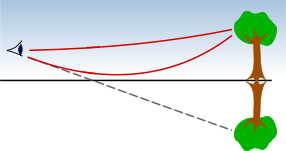
\includegraphics[width=12truecm]{slike/02_Fata1.jpg}
\caption{Zračno zrcaljenje na vročih tleh}
\label{fig:02_Fata1}
\end{figure}
\vglue-0.6truecm
Zgornje zračno zrcaljenje se nasprotno pojavi, 
kadar je spodnja plast zraka izrazito hladnejša od zgornjih plasti. 
Takrat se svetlobni žarki krivijo navzdol (slika~\ref{fig:02_Fata2})
in navidezno sliko predmeta premaknejo nad njegovo dejansko lego. 
Slika je lahko pokončna ali obrnjena, odvisno od oddaljenosti predmeta
in temperature plasti. 
\begin{figure}[h!]
\centering
\includegraphics[width=12truecm]{slike/02_Fata2.jpg}
\caption{Zračno zrcaljenje na hladnejši podlagi (Foto: Craig Clements, Wikimedia)}
\label{fig:02_Fata2}
\end{figure}
\vglue-0.6truecm
Ukrivljena pot žarkov zaradi temperaturnega gradienta v atmosferi
vodi še do enega zanimivega pojava: popačenja oblike Sonca ob sončnem 
zahodu. Ker žarki s spodnjega dela Sonca potujejo po bolj ukrivljeni
poti kot žarki z zgornjega dela, se spodnji rob navidezno premakne navzgor 
in slika Sonca se splošči ali popači.
\begin{figure}[ht]
\centering
\includegraphics[width=5truecm]{slike/02_Sonce.jpg}
\caption{Sonce se ob sončnem zahodu navidezno splošči in njegova oblika popači.}
\label{fig:02_Sonce}
\end{figure}
\vglue-0.6truecm
\section{Transformacije žarkov z matrikami ABCD}
V prejšnjem razdelku smo zapisali žarkovno enačbo v obosnem 
približku (enačba~\ref{eq:02_24}). Ključna parametra za opis trajektorije žarka sta 
oddaljenost od optične osi $z$, ki jo označimo z $x$, in naklonski 
kot žarka glede na optično os, ki ga označimo s $\vartheta$.
Naša naloga je povezati dve točki žarka na različnih mestih v
prostoru in zapisati preslikavo med njima, če je med točkama
optični medij oziroma nek optični element. 
\begin{figure}[ht]
\centering
\def\svgwidth{90truemm} 
\input{slike/02_ABCD0.pdf_tex}
\caption{Pri danem $z$ žarek opišemo z lego $x$ in smerjo $\vartheta$. Spremembo
teh dveh parametrov opišemo s preslikavo.}
\label{fig:01_ABCD0}
\end{figure}

V splošnem vrednosti lege in naklona v točki 2 izrazimo kot 
linearno kombinacijo prvotnih vrednosti v točki 1:
\begin{align}
 x_2 &= A x_1 + B \vartheta_1 \qquad \mathrm{in}  \label{eq:02_29}\\
 \vartheta_2 &=  C x_1 + D\vartheta_1.
 \label{eq:02_30}
\end{align}
Če združimo parametra $x$ in $\vartheta$ v neki točki prostora
v dvodimenzionalni vektor,
lahko preslikavo strnjeno zapišemo v matrični obliki:
\boxeq{eq:02_31}{
\left[\begin{array}{c}
x_2\\
\vartheta_2
\end{array}\right] = 
\left[\begin{array}{cc}
A& B\\
C&D
\end{array}\right]
\left[\begin{array}{c}
x_1\\
\vartheta_1
\end{array}\right]
= M \left[\begin{array}{c}
x_1\\
\vartheta_1
\end{array}\right]\!\!.
}
Matriko $M$ imenujemo transformacijska oziroma prehodna matrika 
vmesnega optičnega medija ali optičnega elementa. 

\begin{example}
\label{ex:ML}
{\bf Matrika ABCD za premik v homogeni snovi s konstantnim lomnim količnikom.} 
Prvi primer naj bo homogena snov, v kateri je lomni količnik konstanten in enak $n$. 
V točki 1 pri $z_1$ naj bosta komponenti vektorja enaki $x_1$ in 
$\vartheta_1$. Poiščimo vrednosti komponent vektorja, 
če se premaknemo za $L$ vzdolž optične osi sistema do $z_2$ 
(slika~\ref{fig:01_ABCD1}). 
\begin{figure}[ht]
\centering
\def\svgwidth{70truemm} 
\input{slike/02_ABCD1.pdf_tex}
\caption{K izračunu matrike ABCD za premik v homogeni snovi}
\label{fig:01_ABCD1}
\end{figure}

Naklon žarka se pri premiku ne spremeni, zato ostane $\vartheta_2 = \vartheta_1$. Spremeni
pa se odmik od optične osi, saj žarek ne potuje vzporedno z osjo $z$. 
Vrednost $x_2$ zapišemo kot:
\begin{equation}
 x_2 = x_1 + (z_2-z_1)\vartheta_1 = x_1 + L\vartheta_1.
\label{eq:02_32}
\end{equation}
Potem zapišemo sistem enačb:
\begin{align}
 x_2 &= 1\cdot x_1 + L\cdot \vartheta_1 \qquad \mathrm{in} \label{eq:02_33}\\
 \vartheta_2 &= 0\cdot x_1 + 1\cdot \vartheta_1.
 \label{eq:02_34}
\end{align}
Iz zapisa razberemo koeficiente matrike $M$ za homogeno snov dolžine $L$:
\begin{equation}
 M = \left[\begin{array}{cc}
1& L\\
0&1
\end{array}\right]\!\!.
 \label{eq:02_35}
\end{equation}
\end{example}

\begin{example}
\label{ex:Mmeja}
{\bf Matrika ABCD za prehod skozi ravno mejo med dvema snovema.} Naj svetloba vpada na 
mejo dveh snovi z različnima lomnima količnikoma $n_1$ in $n_2$. Za izračun 
prehodne matrike izberemo dve točki na žarku: eno tik pred mejo in eno tik za njo. 
Lega žarka se ob tem ne spremeni in $x_2 = x_1$. 
Spremeni pa se naklon žarka. 
\begin{figure}[ht]
\centering
\def\svgwidth{70truemm} 
\input{slike/02_ABCD2.pdf_tex}
\caption{K izračunu matrike ABCD za prehod skozi ravno mejo med dvema snovema}
\label{fig:01_ABCD2}
\end{figure}

Za majhne naklone lahko lomni zakon
(enačba~\ref{eq:lomnizakon}) razvijemo in dobimo:
\begin{equation}
n_1 \vartheta_1 = n_2 \vartheta_2.
 \label{eq:02_36}
\end{equation}
Sistem enačb je potem:
\begin{align}
 x_2 &= 1\cdot x_1 + 0\cdot \vartheta_1 \qquad \mathrm{in} \label{eq:02_37}\\
 \vartheta_2 &= 0\cdot x_1 + \frac{n_1}{n_2}\cdot \vartheta_1.
 \label{eq:02_38}
\end{align}
Matrika $M$ za prehod skozi mejo med dvema snovema je:
\begin{equation}
 M = \left[\begin{array}{cc}
1& 0\\
0&\frac{n_1}{n_2}
\end{array}\right]\!\!.
\label{eq:02_39}
\end{equation}
\end{example}

\begin{example}
\label{ex:MUmeja}
{\bf Matrika ABCD za prehod skozi ukrivljeno mejo med dvema snovema.} V prejšnjem 
primeru je bila meja med snovema z lomnima količnikoma $n_1$ in $n_2$ ravna, zdaj pa 
poglejmo še matriko za prehod skozi ukrivljeno mejo. Krivinski radij mejne ploskve
naj bo $R$, pri čemer $R$ štejemo pozitivno, če je meja konveksna glede na smer
naraščajočega $z$ oziroma če je središče krožnice za mejo med snovema. V primeru, 
da je središče krožnice, ki določa mejo med snovema, pred mejo, je meja konkavna, 
krivinski radij mejne ploskve pa negativen. 

Za izračun matrike ponovno izberemo dve točki, prvo tik pred mejo in 
drugo tik za njo. To pomeni, da se oddaljenost od optične osi
pri prehodu ohranja in $x_1 = x_2$. 

Izračun naklona žarka po prehodu je malo bolj zapleten. Za zapis lomnega 
zakona moramo namreč vpeljati kote glede na normalo na
mejo. Vpadni kot je tako $\alpha = \vartheta_1 + \varphi$, lomni kot pa 
$\beta = \vartheta_2 + \varphi$ (glej sliko~\ref{fig:02_ABCD3}).
Privzamemo, da je ukrivljenost meje dovolj majhna oziroma da so žarki
dovolj blizu optične osi, da velja zveza:
\begin{equation}
 \sin \varphi = \frac{x_1}{R} \approx \varphi.
 \label{eq:02_40}
\end{equation}
\begin{figure}[!h]
\centering
\def\svgwidth{70truemm} 
\input{slike/02_ABCD3.pdf_tex}
\caption{K izračunu matrike ABCD za prehod skozi ukrivljeno mejo med dvema snovema}
\label{fig:02_ABCD3}
\end{figure}

Zapišemo lomni zakon,
pri čemer privzamemo, da so vsi koti majhni:
\begin{equation}
n_1 (\vartheta_1 + \varphi) = n_2 (\vartheta_2 + \varphi).
\label{eq:02_41}
\end{equation}
Od tod izračunamo kot $\vartheta_2$:
\begin{equation}
 \vartheta_2 = \frac{n_1-n_2}{n_2}\varphi + \frac{n_1}{n_2} \vartheta_1.
 \label{eq:02_42}
 \end{equation}
Če $\varphi$ izrazimo iz enačbe~(\ref{eq:02_40}), zapišemo transformacijo koordinat:
\begin{align}
 x_2 &= 1\cdot x_1 + 0\cdot \vartheta_1 \qquad \mathrm{in} \\
 \vartheta_2 &= \frac{n_1-n_2}{n_2R}\cdot x_1 + \frac{n_1}{n_2}\cdot \vartheta_1.
 \label{eq:02_43}
\end{align}
Razberemo matriko $M$ za prehod skozi ukrivljeno mejo med dvema snovema:
\begin{equation}
M = \left[\begin{array}{cc}
1& 0\\
\frac{n_1-n_2}{n_2R}&\frac{n_1}{n_2}
\end{array}\right]\!\!.
 \label{eq:02_44}
\end{equation}
V limitnem primeru, ko gre $R \to \infty$, se matrika prevede na matriko za
prehod skozi ravno mejo (glej primer~\ref{ex:Mmeja}).
\end{example}

Izračunajmo še determinanto izpeljanih matrik ABCD. Na splošno velja, da
je determinanta matrike ABCD enaka razmerju lomnih količnikov začetne in 
končne snovi. Če je lomni količnik snovi na koncu enak
kot na začetku (primer~\ref{ex:ML}), je $\det(M) = 1$, v nasprotnem primeru 
(primera~\ref{ex:Mmeja} in \ref{ex:MUmeja}) je $\det(M) = n_1/n_2$.

Do zdaj smo obravnavali matrike za posamezne prehode. Poglejmo, kako izračunamo
prehodno matriko za primer, če svetloba potuje skozi več elementov zapored. V tem
primeru se pokažeta izjemna praktičnost in uporabnost zapisa z matrikami, saj ob prehodu svetlobe skozi 
več elementov matrike za te elemente preprosto zmnožimo. Paziti moramo seveda
na vrsti red: matriko za element, na katerega vpade svetloba najprej, zapišemo
najbolj desno, to je najbliže vektorju, ki opisuje vpadno svetlobo. Celoten prehod
spet opiše ena sama matrika:
\begin{equation}
\left[\begin{array}{c}
x_N\\
\vartheta_N
\end{array}\right] 
= \tilde{M} \left[\begin{array}{c}
x_1\\
\vartheta_1
\end{array}\right]\!\!,
 \label{eq:02_45}
\end{equation}
pri čemer je:
\begin{equation}
\tilde{M} = M_N \cdot M_{N-1}~...~M_2 \cdot M_1.
 \label{eq:02_46}
\end{equation}
\begin{figure}[ht]
\centering
\def\svgwidth{100truemm} 
\input{slike/02_MMM.pdf_tex}
\caption{Prehod žarka skozi več optičnih elementov zapišemo kot produkt matrik posameznih prehodov.
Pri tem moramo paziti na vrstni red zapisa matrik.}
\label{fig:01_MMM}
\end{figure}

\section{Preslikave z lečami}
\label{chap:lecje}
Uporabimo matrike ABCD za izračun prehoda svetlobe skozi tanko lečo. Matriko
za prehod zapišemo kot produkt dveh matrik: prve, ki opiše
prehod skozi prvo ukrivljeno ploskev s krivinskim radijem $R_1$, 
in druge, ki opiše prehod skozi izhodno ukrivljeno ploskev s 
krivinskim radijem $R_2$. Za bikonveksno lečo, na primer, je 
$R_1>0$ in $R_2<0$ (glej sliko~\ref{fig:02_tankaleca}). 
Lomni količnik leče naj bo $n_2$ in snovi okoli leče 
(navadno je to zrak) $n_1$. Zanima nas, kako se vektor $(x_1, \vartheta_1)$ 
preslika v $(x_2, \vartheta_2)$.
\begin{figure}[!h]
\centering
\def\svgwidth{100truemm} 
\input{slike/02_tankaleca.pdf_tex}
\caption{K izračunu matrike ABCD za prehod skozi tanko bikonvkesno lečo}
\label{fig:02_tankaleca}
\end{figure}

Izračunajmo najprej matriko za prehod skozi lečo. Ker smo privzeli, da je leča tanka, 
vmesne matrike za premik po steklu ne zapišemo. Z upoštevanjem enačbe~(\ref{eq:02_44})
dobimo:
\beq
 M = \left[\begin{array}{cc}
1& 0\\
\frac{n_2-n_1}{n_1R_2}&\frac{n_2}{n_1}
\end{array}\right]\cdot 
\left[\begin{array}{cc}
1& 0\\
\frac{n_1-n_2}{n_2R_1}&\frac{n_1}{n_2}
\end{array}\right] = 
\left[\begin{array}{cc}
1& 0\\
\frac{n_2-n_1}{n_1}\left(\frac{1}{R_2}-\frac{1}{R_1}\right)&1
\end{array}\right]\!\!.
\label{eq:02_47}
\eeq
Vpeljemo parameter $f$, za katerega velja:
\beq
\frac{1}{f} = -\frac{n_2-n_1}{n_1}\left(\frac{1}{R_2}-\frac{1}{R_1}\right)\!\!.
\label{eq:02_48}
\eeq
Element matrike $C$ je tako enak $-1/f$. Fizikalni pomen tega parametra
bomo kmalu spoznali.

Uporabimo izračunano matriko za opis prehoda svetlobe skozi lečo. Naj žarek izhaja iz 
predmeta, ki je na oddaljenosti $a$ od leče, opazujemo pa ga na razdalji
$b$ za lečo. Za celotno pot žarka moramo zmnožiti tri matrike: matriko za 
premik do leče, matriko za prehod skozi lečo in matriko za premik do opazovalca.
Dobimo:
\beq
M = 
\left[\begin{array}{cc}
1& b\\
0&1
\end{array}\right]\cdot
\left[\begin{array}{cc}
1& 0\\
-\frac{1}{f}&1
\end{array}\right]
\cdot
\left[\begin{array}{cc}
1& a\\
0&1
\end{array}\right]
= 
\left[\begin{array}{cc}
1-\frac{b}{f}& a+b-\frac{ab}{f}\\
-\frac{1}{f}&1-\frac{a}{f}
\end{array}\right]\!\!.
\label{eq:02_49}
\eeq
Najprej poiščimo pomen parametra $f$, ki smo ga vpeljali z enačbo~(\ref{eq:02_48}).
Poglejmo, v kaj se preslikajo žarki, ki na neki oddaljenosti od osi $x_1$ vpadajo na lečo 
vzporedno z optično osjo $z$:
\beq
\left[\begin{array}{c}
x_2\\
\vartheta_2
\end{array}\right] =
\left[\begin{array}{cc}
1-\frac{b}{f}& a+b-\frac{ab}{f}\\
-\frac{1}{f}&1-\frac{a}{f}
\end{array}\right] \cdot
\left[\begin{array}{c}
x_1\\
0
\end{array}\right] = 
\left[\begin{array}{c}
\left(1-\frac{b}{f}\right)x_1\\
-\frac{x_1}{f}
\end{array}\right]\!\!.
\label{eq:02_51}
\eeq
Vsi vzporedni vpadni žarki se zberejo v eni točki, kadar velja $1-b/f = 0$ in $b=f$. 
Vzporedni žarki se torej zberejo na oddaljenosti $f$, zato 
parameter $f$ prestavlja goriščno razdaljo leče. 
Ker navadno obravnavamo lečo v zraku, enačbo~(\ref{eq:02_48}) za izračun 
goriščne razdalje leče poenostavljeno zapišemo  kot:
\boxeq{eq:goriscna}{
\frac{1}{f} = \left(n-1\right)\left(\frac{1}{R_1}-\frac{1}{R_2}\right)\!\!,
}
pri čemer je $n$ lomni količnik stekla, iz katerega je leča narejena, $R_1$ in $R_2$ pa 
sta krivinska radija mejnih ploskev leče. Ne smemo pozabiti, da je za bikonveksno lečo $R_2 <0$.

Vrnimo se k izračunani matriki (enačba~\ref{eq:02_49}).
Da na desni strani leče nastane slika predmeta, se morajo 
žarki, ki izhajajo iz ene točke predmeta na levi, zbrati
v eni točki na desni strani leče, neodvisno od njihovega naklona.
Ta zahteva je izpolnjena le ob pogoju, da je element matrike prehoda $B = 0$ in velja:
\boxeq{eq:PreslikavaLeca}{
\frac{1}{f} = \frac{1}{a}+\frac{1}{b}.
}
Dobili smo enačbo leče, ki povezuje lego predmeta z lego njegove slike.

Razmerje med velikostima slike $x_2$ in predmeta $x_1$ določa
element matrike $A$, ki ga z upoštevanjem enačbe~(\ref{eq:PreslikavaLeca})
zapišemo kot:
\beq
A= 1-\frac{b}{f} = 1 - b\left(\frac{1}{a}+\frac{1}{b}\right) = -\frac{b}{a}.
\label{eq:02_50}
\eeq
Povečava leče je tako enaka:
\boxeq{eq:PovecavaLece}{
\frac{x_2}{x_1} =-\frac{b}{a}.
}
Negativni predznak pomeni, da je slika predmeta desno od leče obrnjena na glavo
(glej sliko~\ref{fig:02_slikazaleco}).
\begin{figure}[!ht]
\centering
\def\svgwidth{140truemm} 
\input{slike/02_slikazaleco.pdf_tex}
\caption{Kadar je predmet bolj oddaljen od leče kot je goriščna razdalja ($a>f$),
nastane obrnjena prava slika desno od leče. 
V tem primeru sta $a,b>0$ (levo). Če je predmet blizu leče in velja $a<f$,
nastane pokončna navidezna slika na isti strani, kot je predmet. V tem primeru velja $a>0$ in $b<0$.}
\label{fig:02_slikazaleco}
\end{figure}

Če je predmet oddaljen od leče več kot je goriščna razdalja, nastane na desni
strani na glavo obrnjena prava slika, ki jo lahko projiciramo na zaslon. Če je 
predmet blizu leče in velja $a<f$, je po enačbi~(\ref{eq:PreslikavaLeca}) 
vrednost $b$ negativna. Žarki desno od leče se ne sekajo, temveč se sekajo podaljški 
žarkov levo od leče. Slika predmeta je tako le navidezna in je
ne moremo projicirati na zaslon. Povečava take slike je pozitivna, 
kar pomeni, da je navidezna slika pokončno obrnjena.

Opisani izračun je bil narejen na primeru bikonveksne leče, vendar velja
povsem splošno za poljubno tanko lečo. Paziti moramo le na predznake krivinskih
radijev vstopne in izstopne ploskve. Če je ena stranica leče ravna, je 
njen krivinski radij neskončen. 

\begin{example}{\bf Preslikava z dvema zaporednima lečama.}
Poglejmo prehod svetlobe skozi dve zaporedni tanki leči z goriščnima
razdaljama $f_1$ in $f_2$, ki sta na medsebojni oddaljenosti $s$.
\begin{figure}[!h]
\centering
\def\svgwidth{100truemm} 
\input{slike/02_dveleci.pdf_tex}
\caption{Prehod svetlobe skozi sistem dveh tankih leč}
\label{fig:02_lecje}
\end{figure}

Matriko sistema dveh leč za prehod z leve proti desni zapišemo kot:
\beq
M = 
\left[\begin{array}{cc}
1& 0\\
-\frac{1}{f_2}&1
\end{array}\right]\cdot 
\left[\begin{array}{cc}
1& s\\
0&1
\end{array}\right]\cdot
\left[\begin{array}{cc}
1& 0\\
-\frac{1}{f_1}&1
\end{array}\right] = 
\left[\begin{array}{cc}
1-\frac{s}{f_1}& s\\
-\frac{1}{f_1}-\frac{1}{f_2}+\frac{s}{f_1f_2}&1-\frac{s}{f_2}
\end{array}\right]\!\!.
\label{eq:02_54}
\eeq
Izračunajmo goriščno razdaljo takega sistema in lego gorišča
na desni strani. Za opis  žarkov desno
od sistema je treba matriko prehoda pomnožiti še z matriko premika za $d$. 

Naj bodo vpadni žarki vzporedni z optično osjo in jih zapišemo 
v obliki vektorja $(x_1,0)$. Izhodne žarke potem izračunamo kot:
\beq
\left[\begin{array}{c}
x_2\\
\vartheta_2
\end{array}\right]
 = 
\left[\begin{array}{cc}
1& d\\
0&1
\end{array}\right]
\cdot
\left[\begin{array}{cc}
A& B\\
C&D
\end{array}\right]\cdot 
\left[\begin{array}{c}
x_1\\
0
\end{array}\right] = 
\left[\begin{array}{c}
\left(A+dC\right)x_1\\
Cx_1
\end{array}\right]\!\!,
\label{eq:02_55}
\eeq
pri čemer so elementi matrike ABCD podani z enačbo~(\ref{eq:02_54}). 
Po definiciji se vzporedni vpadni žarki po prehodu sekajo v gorišču, 
zato je naklon izhodnega žarka $\vartheta_2 = -x_1/f$ in $C = -1/f$. 
Od tod razberemo goriščno razdaljo sistema:
\boxeq{eq:lecje}{
\frac{1}{f} = \frac{1}{f_1} + \frac{1}{f_2} - \frac{s}{f_1f_2}.
}
Oddaljenost gorišča od desne leče določimo iz pogoja, da je v gorišču $x_2 = 0$. Dobimo:
\beq
d = -\frac{A}{C} = \frac{f_1f_2-sf_2}{f_1+f_2-s}.
\label{eq:02_56}
\eeq
Pri sestavu leč pogosto vpeljemo glavno ravnino. To je ravnina, pravokotna
na optično os, v kateri bi 
bila postavljena nadomesta tanka leča. Dobimo jo tako, da poiščemo 
presečišče žarkov, ki vpadajo na sistem vzporedno z optično osjo, 
in žarkov ali njihovih podaljškov, ki iz sestava izhajajo desno od lečja. 
Ko poznamo lego gorišča, je lego glavne ravnine preprosto določiti, 
saj vemo, da je glavna ravnina od gorišča oddaljena ravno za goriščno razdaljo.

Račun je bil narejen za prehod svetlobe iz
leve proti desni strani. Ker se leči v splošnem razlikujeta in matrike
ne komutirajo, je prehod z desne proti levi drugačen. Skupna goriščna
razdalja ostane enaka, premakneta pa se lega gorišča in glavna ravnina.
\end{example}

\begin{example}{\bf Preslikava z debelo lečo}
Matriko za prehod skozi debelo lečo s krivinskima radijema
$R_1$ in $R_2$ ter debelino $d$ lahko neposredno izračunamo
z množenjem treh matrik: matrike za prehod skozi ukrivljeno vstopno 
ploskev, matrike za premik znotraj leče in matrike za prehod skozi 
ukrivljeno izstopno ploskev, pri čemer naj bo $n_1 = 1$:
\beq
M = 
\left[\begin{array}{cc}
1& 0\\
\frac{n-1}{R_2}&n
\end{array}\right]
\cdot
\left[\begin{array}{cc}
1& d\\
0&1
\end{array}\right]
\cdot
\left[\begin{array}{cc}
1& 0\\
\frac{1-n}{nR_1}&\frac{1}{n}
\end{array}\right]\!\!.
\label{eq:02_52}
\eeq
Matriko za prehod lahko izračunamo tudi drugače, na podlagi podobnosti 
s sistemom dveh leč. Debelo lečo razdelimo
na tri dele: vstopno plankonveksno lečo, plast stekla in izstopno plankonkavno lečo.
Goriščni razdalji leč zapišemo z uporabo enačbe~(\ref{eq:goriscna}), pri čemer upoštevamo, 
da je krivinski radij ravne stranice neskončen:
\beq
\frac{1}{f_1} = (n-1)\frac{1}{R_1}\qquad \mathrm{in} \qquad \frac{1}{f_2} = -(n-1)\frac{1}{R_2}.
\label{eq:02_53}
\eeq
Pri vmesnemu prehodu skozi steklo moramo upoštevati tudi njegov
lomni količnik. Na splošno se pri prehodu žarka skozi plast snovi debeline $d$
z lomnim količnikom $n$ matrika zapiše kot:
\beq
M = 
\left[\begin{array}{cc}
1& 0\\
0&n
\end{array}\right]\cdot
\left[\begin{array}{cc}
1& d\\
0&1
\end{array}\right]\cdot
\left[\begin{array}{cc}
1& 0\\
0&\frac{1}{n}
\end{array}\right] = 
\left[\begin{array}{cc}
1& \frac{d}{n}\\
0&1
\end{array}\right]\!\!.
\label{eq:02_54a}
\eeq
Efektivna dolžina poti skozi snov je torej skrajšana za faktor $n$.

Ugotovitve vstavimo v enačbo za lečje (enačba~\ref{eq:02_54}) in dobimo:
\beq
M = 
\left[\begin{array}{cc}
1-\frac{d}{nf_1}& \frac{d}{n}\\
-\frac{1}{f_2}-\frac{1}{f_1}+\frac{d}{nf_1f_2}&1-\frac{d}{nf_2}
\end{array}\right]\!\!.
\label{eq:02_53a}
\eeq
Hitro lahko preverimo, da dobimo isti rezultat, če zmnožimo matrike v enačbi~(\ref{eq:02_52}).
Prav tako hitro preverimo tudi, da je izračunana matrika za debelo lečo v limitnem 
primeru $d \to 0$ enaka matriki za prehod skozi tanko lečo. 
\end{example}

\begin{remark}
Vsi izračuni so bili narejeni v obosnem 
približku, v katerem je smer žarka le malo odstopala od smeri optične osi. V praksi se lahko 
zgodi, da ta pogoj ni izpolnjen in preslikani žarki se ne sekajo v isti točki. Ta pojav opišemo
kot napako leče. Poleg navedenega je še vrsta drugih razlogov, na primer nepravilnost leče 
ali odvisnost lomnega količnika leče od valovne dolžine, ki vodijo do popačenja slike. 
Marsikatero od teh nepravilnost lahko odpravimo tako, da namesto ene same leče uporabimo 
zapleten sestav leč, ki deluje podobno kot ena idealna leča. Fotografski objektivi so 
tako navadno sestavljeni iz vsaj treh do štirih leč, zapletenejši tudi več kot petnajstih.
\end{remark}
 
\section{Odboj svetlobe na zrcalih}
Opis odboja na ravnih zrcalih je 
preprost: vse slike posamezne točke se po odboju zberejo v eni točki, 
navidezna slika, ki pri tem nastane, pa je enako velika in enako obrnjena kot predmet.
Matrika ABCD, ki opiše odboj od takega zrcala, je identiteta. Pri tem se moramo
zavedati, da žarek po odboju spremeni smer in z njim tudi os $z$.

Poiščimo še matriko za odboj od ukrivljenega zrcala. Naj bo krivinski radij zrcala
$R$, pri čemer za konkanvna zrcala, pri katerih sta predmet in krivinsko središče
na isti strani zrcala, velja $R>0$. Pri odboju na zrcalu se lega žarka ne spremeni, zato 
je $x_2 = x_1 = x$. Od tod takoj izračunamo prva dva elementa matrike ABCD: $A = 1$ in 
$B=0$. Pri transformaciji kota si pomagamo s sliko~\ref{fig:02_zrcalo}. 
\begin{figure}[!h]
\centering
\def\svgwidth{80truemm} 
\input{slike/02_zrcalo.pdf_tex}
\caption{K izračunu matrike ABCD za odboj na kroglastem zrcalu}
\label{fig:02_zrcalo}
\end{figure}

Naj bo $\alpha$ kot med optično osjo in zveznico med središčem krožnice in točko, 
v kateri vpada žarek na zrcalo. Vpadni žarek naj se širi pod kotom $\vartheta_1$, tako da
je vpadni kot glede na normalo na zrcalo enak $\alpha -\vartheta_1$. Kot, pod katerim 
se žarek odbije glede na vodoravnico naj bo $-\vartheta_2$, tako da je odbojni kot glede
na normalo na zrcalo enak $\vartheta_2 - \alpha$. Po odbojnem zakonu sta vpadni in odbojni
kot enaka, zato:
\beq
\alpha - \vartheta_1= \vartheta_2-\alpha.
\label{eq:02_60}
\eeq
Za majhne vrenosti velja $\alpha \approx x/R$, od koder sledi:
\beq
-\vartheta_2 = \vartheta_1 - \frac{2}{R}x.
\label{eq:02_61a}
\eeq
Od tod lahko razberemo elementa matrike $C = -2/R$ in $D = 1$. Celotna matrika za odboj 
na zrcalu je potem:
\begin{equation}
 M = \left[\begin{array}{cc}
1& 0\\
-\frac{2}{R}&1
\end{array}\right]\!\!.
 \label{eq:02_62}
\end{equation}
Naj žarek vpada na zrcalo v smeri vzporedno z optično osjo $(x_1, 0)$:
\begin{equation}
\left[\begin{array}{c}
x_2\\
\vartheta_2
\end{array}\right]
= \left[\begin{array}{cc}
1& 0\\
-\frac{2}{R}&1
\end{array}\right]\cdot
\left[\begin{array}{c}
x_1\\
0
\end{array}\right] = 
\left[\begin{array}{c}
x_1\\
-\frac{2x_1}{R}
\end{array}\right]\!\!.
 \label{eq:02_63}
\end{equation}
Žarek tik po odboju svoje lege ne spremeni, spremeni pa svojo smer.
Ker je usmerjen proti gorišču, je podobno kot
pri obravnavi leče njegova smer $\vartheta_2 = -x_1/f$. 
Od tod razberemo goriščno razdaljo krogelnega zrcala kot:
\boxeq{eq:02_zrcalof}{
f = \frac{R}{2}.
}
Preslikajmo še poljuben predmet, ki je na razdalji $a$ od temena zrcala, in poiščimo
pogoj za nastanek njegove slike na mestu $b$:
\beq
M = 
\left[\begin{array}{cc}
1& b\\
0&1
\end{array}\right]\cdot
\left[\begin{array}{cc}
1& 0\\
-\frac{2}{R}&1
\end{array}\right]
\cdot
\left[\begin{array}{cc}
1& a\\
0&1
\end{array}\right]
= 
\left[\begin{array}{cc}
1-\frac{2b}{R}& a+b-\frac{2ab}{R}\\
-\frac{2}{R}&1-\frac{2a}{R}
\end{array}\right]\!\!.
\label{eq:02_64}
\eeq
Da po odboju nastane ostra slika predmeta, mora biti element matrike $B=0$ 
(glej enačbo~\ref{eq:PreslikavaLeca}). To velja, kadar je izpolnjen pogoj:
\boxeq{eq:PreslikavaZrcalo}{
\frac{1}{f} = \frac{2}{R} = \frac{1}{a}+\frac{1}{b}.
}
Pri konkavnem zrcalu je $R>0$, vrednosti $a$ in $b$ pa sta pozitivni, če sta 
na isti strani kot krivinsko središče. Če je predmet od zrcala oddaljen več 
kot gorišče, je njegova slika prava in obrnjena. Vrednost $b$ je v tem primeru pozitivna.
Za predmete, za katere velja $a<f$, se odbiti žarki ne sekajo. Narisati
moramo podaljške žarkov in slika nastane na mestu, kjer se sekajo podaljški odbitih
žarkov (slika~\ref{fig:02_zrcaloodboj}).
\begin{figure}[!ht]
\centering
\def\svgwidth{140truemm} 
\input{slike/02_zrcaloodboj.pdf_tex}
\caption{Kadar je predmet bolj oddaljen od zrcala kot je goriščna razdalja ($a>f$),
nastane na isti strani zrcala obrnjena prava slika. 
V tem primeru sta $a,b>0$ (levo). Če je predmet blizu zrcala in velja $a<f$,
nastane pokončna navidezna slika na drugi strani zrcala. V tem primeru velja $a>0$ in $b<0$.}
\label{fig:02_zrcaloodboj}
\end{figure}

Povsem enako kot pri lečah izračunamo tudi povečavo zrcala. Element matrike $A$
preoblikujemo z upoštevanjem enačbe~(\ref{eq:PreslikavaZrcalo}) in dobimo:
\boxeq{eq:PovecavaZrcala}{
\frac{x_2}{x_1} =-\frac{b}{a}.
}
Gornji izračun je bil narejen na primeru konkavnega zrcala. Vendar so rezultati
povsem splošni in veljajo za vsa ukrivljena zrcala, pri čemer
je krivinski radij konveksnih zrcal negativen, ravnih zrcal pa neskončen. 

Z vpeljavo matrike za preslikavo z zrcalom lahko na preprost način v izračun
poti žarka v obosnem približku vključimo tudi zrcala. Vendar ne pozabimo, da se
pri odboju na zrcalu spremeni smer optične osi, kar moramo upoštevati v nadaljnjem računu.

\section{Preproste optične naprave}
Za konec si oglejmo še delovanje nekaterih optičnih naprav. Obravnavali jih bomo 
v najpreprostejši, a zato najnazornejši obliki. Izhajamo iz sestava dveh leč, ki 
smo jih obravnavali v razdelku~\ref{chap:lecje}. 

\subsection*{Razširjevalec snopov}
Spomnimo se matričnega zapisa prehoda skozi sistem dveh leč z goriščnima razdaljama
$f_1$ in $f_2$, ki sta na medsebojni razdalji $s$ (enačba~\ref{eq:02_54}). Poiščimo
pogoj, pri katerem so tako vpadni kot izhodni žarki iz sistema vzporedni z optično osjo.
Da je ta pogoj izpolnjen pri vseh vstopnih $x$, mora biti 
element prehodne matrike $C$ enak nič:
\beq
C = -\frac{1}{f_1}-\frac{1}{f_2} + \frac{s}{f_1f_2} = 0,
\label{eq:02_65}
\eeq
od koder sledi:
\beq
s = f_1 + f_2.
\label{eq:02_57}
\eeq
Vzporedni vpadni žarki izhajajo kot vzporedni žarki, kadar goriščni ravnini leč sovpadata.
Povečava takega sistema je z upoštevanjem enačbe~(\ref{eq:02_57}) enaka:
\beq
\frac{x_2}{x_1} = A = 1 - \frac{s}{f_1} = \frac{f_2}{f_1}.
\label{eq:02_58}
\eeq
Če je goriščna razdalja druge leče večja od goriščne razdalje prve leče, 
lahko širino snopa vzporednih vpadajočih žarkov močno povečamo -- žarek razširimo.
Tako napravo zato imenujemo razširjevalec snopov in je zelo uporabna v optičnih laboratorijih.

\subsection*{Teleskop in daljnogled}
Teleskop in daljnogled uporabljamo za opazovanje zelo oddaljenih predmetov, 
zato lahko privzamemo, da vpadajo žarki s teh predmetov na optični sistem praktično vzporedno. 
Naj bo zorni kot, pod katerim vidimo oddaljen predmet brez teleskopa, enak $\vartheta_1$.
Da so vzporedni tudi izhodni žarki, uporabimo lečje, pri katerem je razdalja med 
lečama enaka vsoti goriščnih razdalj obeh leč. Vstopno lečo imenujemo objektiv, 
izstopno lečo pa okular. Pravo sliko, ki nastane po prehodu objektiva,
opazujemo z okularjem, nastala slika pa je v tej preprosti izvedbi obrnjena. 
\begin{figure}[ht]
\centering
\def\svgwidth{100truemm} 
\input{slike/02_teleskop.pdf_tex}
\caption{V preprostem teleskopu gorišči leč sovpadata. V goriščni ravnini nastane 
slika predmeta, ki jo opazujemo z okularjem.}
\label{fig:02_teleskop}
\end{figure}
\vglue-10truemm
Poiščimo še povečavo takega preprostega teleskopa. Vpadni žarek, ki gre skozi središče
objektiva, je enak $(0,\vartheta_1)$. Izračunajmo izhodni žarek po prehodu skozi 
optični sistem, ki ga v splošnem opisuje matrika (enačba~\ref{eq:02_54}). Dobimo:
\beq
\left[\begin{array}{c}
x_2\\
\vartheta_2
\end{array}\right] = 
\left[\begin{array}{cc}
1-\frac{f_1+f_2}{f_1}& f_1+f_2\\
-\frac{1}{f_1}-\frac{1}{f_2}+\frac{f_1+f_2}{f_1f_2}&1-\frac{f_1+f_2}{f_2}
\end{array}\right] 
\cdot
\left[\begin{array}{c}
0\\
\vartheta_1
\end{array}\right]  = 
\left[\begin{array}{c}
(f_1+f_2) \vartheta_1\\
-\frac{f_1}{f_2}\vartheta_1
\end{array}\right]\!\!.
\label{eq:02_66}
\eeq
Zorni kot, pod katerim vidimo izhodne žarke $\vartheta_2$ je enak vstopnemu zornemu kotu, 
pomnoženemu z razmerjem goriščnih razdalj leč:
\boxeq{eq:teleskop}{
\vartheta_2 = -\frac{f_1}{f_2}\vartheta_1.
}
Če je goriščna razdalja objektiva $f_1$ večja
od goriščne razdalje okularja $f_2$, vidimo oddaljen predmet povečan.
Negativni predznak pri razmerju pomeni, da vidimo sliko obrnjeno na glavo. 

V praksi so teleskopi sestavljeni precej bolj zapleteno. Lahko so sestavljeni iz kombinacije
konveksnih in konkavnih leč, skoraj vedno pa vsebujejo tudi zrcala, saj je izdelava
velikih ukrivljenih zrcal preprostejša od izdelave velikih leč. 

\subsection*{Mikroskop}
Za opazovanje majhnih predmetov uporabimo mikroskop. Preprost mikroskop je sestavljen
iz dveh leč: objektiva, ki je bliže predmetu, in okularja, ki je bliže očesu 
(slika~\ref{fig:02_mikroskop}). Obe leči 
naj bosta zbiralni z goriščnima razdaljama $f_1$ in $f_2$ na oddaljenosti $s$. Predmet
postavimo blizu objektivu, vendar dovolj daleč, da velja $a>f_1$. Za objektivom 
nastane prava, povečana in obrnjena slika predmeta. Nastalo sliko opazujemo z okularjem, 
tako da so izhodni žarki praktično vzporedni in izhajajo iz sistema pod kotom $\vartheta_2$.
\begin{figure}[ht]
\centering
\def\svgwidth{100truemm} 
\input{slike/02_mikroskop.pdf_tex}
\caption{Preprost mikroskop je sestavljen iz dveh leč. Predmet je blizu objektivu, sliko
predmeta opazujemo z okularjem.}
\label{fig:02_mikroskop}
\end{figure}

Izračunajmo še povečavo preprostega mikroskopa, sestavljena iz dveh zbiralnih leč. Izhajamo
iz matrike za prehod skozi lečje (enačba~\ref{eq:02_54}). Vstopni žarek izberemo vzporeden
z optično osjo $(x_1, 0)$, izhodni pa naj bo $(0, \vartheta_2)$. Dobimo:
\beq
\left[\begin{array}{c}
0\\
\vartheta_2
\end{array}\right] = 
\left[\begin{array}{cc}
1-\frac{s}{f_1}& s\\
-\frac{1}{f_1}-\frac{1}{f_2}+\frac{s}{f_1f_2}&1-\frac{s}{f_2}
\end{array}\right] 
\cdot
\left[\begin{array}{c}
x_1\\
0
\end{array}\right]  = 
\left[\begin{array}{c}
\left(1-\frac{s}{f_1}\right)x_1\\
\left(\frac{s}{f_1f_2}-\frac{1}{f_1}-\frac{1}{f_2}\right)x_1
\end{array}\right]\!\!.
\label{eq:02_67}
\eeq
Vpeljemo $d$ kot razdaljo med notranjimi gorišči mikroskopa
$d= s -f_1-f_2$ in izračunamo zorni kot, pod katerim opazujemo predmet:
\beq
\vartheta_2 = \frac{x_1 d}{f_1f_2}.
\label{eq:02_69}
\eeq
Povečavo mikroskopa vpeljemo glede na zorni kot, pod katerim 
normalno vidimo predmet s prostim očesom, to je:
\beq
\vartheta_0 = \frac{x_1}{a_0},
\label{eq:02_70}
\eeq
pri čemer je po dogovoru normalna vidna razdalja $a_0 = 25~\si{cm}$.
Povečava mikroskopa je potem razmerje zornih kotov:
\beq
\frac{\vartheta_2}{\vartheta_0} = \frac{a_0d}{f_1f_2}.
\eeq

\subsection*{Oko in korekcijska očala}
Človeško oko ima na vstopni strani bikonveksno lečo, ki vpadno 
svetlobo zbere na mrežnici na zadnji strani očesa. 
Goriščna razdalja očesne leče je spremenljiva, da se lahko 
prilagaja za opazovanje tako bližnjih kot oddaljenih
predmetov. 

Če slika predmeta, ki nastane po prehodu skozi očesno lečo,
ne nastane točno na mrežnici, oseba za oster vid potrebuje korekcijska očala.
Daljnovidnost nastopi, kadar slika preslikanih predmetov nastane
za mrežnico. Oseba oddaljene predmete vidi ostro, očesna leča 
pa ne more imeti dovolj kratke goriščne razdalje, da bi nastala ostra 
slika predmetov, ki so na majhnih oddaljenostih od očesa. Vid popravimo z očali z 
zbiralno lečo. Po drugi strani pri kratkovidnih osebah slika
oddaljenih predmetov nastane pred mrežnico, saj očesna leča 
ne more doseči dovolj velikih goriščnih razdalj. Vid popravimo
z razpršilno lečo. 

\begin{remark}
 Kadar govorimo o vidu in korekcijskih očalih, navadno vpreljemo
 še eno praktično fizikalno količino. Namesto goriščne razdalje
 leče $f$ vpeljemo inverzno goriščno razdaljo, ki jo imenujemo 
 lomnost $\mathcal{D}$. Ker smo pri sestavu leč seštevali inverzne
 vrednosti goriščnih razdalj, lomnost leč preprosto seštejemo. 
 Enota za lomnost je dioptrija, pri čemer velja $1~\mathrm{dioptrija} = 
 1~\si{m}^{-1}$.
\end{remark}

\section{Primeri leč in zrcal}
Poglejmo nekaj primerov leč in zrcal, ki jih srečujemo v vsakdanu. Zbiralne leče
(navadno bikonveksne) uporabljamo kot lupe za povečavo pri branju ali 
natančnem delu. Kot zbiralna leča delujejo tudi kapljice vode, okrogli 
kozarci, napolnjeni z vodo, ali steklene krogle. Posebej zanimive so zbiralne leče
v svetilnikih, ki svetlobo z majhnega svetila preslikajo v vzporeden snop svetlobe, ki 
je viden od zelo daleč. Ker bi bile navadne plankonveksne leče prevelike in pretežke, se
v svetilnikih uporablja tako imenovane Fresnelove leče. Sestavljene
so iz kolobarjev, ki imajo enako ukrivljenost kot navadna leča, le da so bistveno
tanjši in zato leča lažja. Razpršilne leče se med drugih uporabljajo v vratnih kukalih. 

\begin{figure}[ht]
\centering
\includegraphics[width=7truecm]{slike/02_photos_lupa.jpg}\hfill
\includegraphics[width=7truecm]{slike/02_photos_kapljice.jpg}
\caption{Drobni tisk na bankovcu vidimo šele z uporabo zbiralne leče (levo). 
Drobne kapljice na zaslonu telefona delujejo kot povečevalna lupa in lahko 
razločimo posamezne rdeče, zelene in modre piksle v prikazovalniku (desno).}
\label{fig:02_photos-1}
\end{figure}

\begin{figure}[!ht]
\centering
\includegraphics[height=7truecm]{slike/02_photos_kozarec.jpg}\hfill

\includegraphics[height=7truecm]{slike/02_FresnelLeca.png}\hfill
\includegraphics[height=7truecm]{slike/02_photos_svetilnik.jpg}
\caption{Kozarec, napolnjen z vodo, deluje kot zbiralna leča in 
sliko obrne (levo). Shema Fresnelove leče: na posameznih
kolobarjih je enaka ukrivljenost kot na navadni leči, vendar je celotna 
leča tanjša in lažja (sredina). Fresnelova leča na svetilniku ustvari široke 
snope svetlobe, ki so vidni od daleč (desno).}
\label{fig:02_photos-2}
\end{figure}
\vglue-1truecm
\begin{figure}[!ht]
\centering
\includegraphics[width=8truecm]{slike/02_photos_peephole.jpg}
\caption{Vratno kukalo uporablja razpršilne leče, da zajamejo čim večjo sliko (levo).}
\label{fig:02_photos-3}
\end{figure}

\newpage
Konveksna zrcala se uporabljajo na primer v avtomobilih kot vzvratna ali v prometu kot
cestna ogledala, da povečamo vidno polje. Podobno delujejo tudi novoletne 
okrasne bunkice ali žlica s hrbtne strani. Konkavna zrcala najdemo v
avtomobilskih žarometih, da zberejo čim več izsevane svetlobe, in za zobozdravniška
ali kozmetična zrcala, da povečajo sliko. Kot konkavno zrcalo deluje tudi 
sprednja stran žlice.

\begin{figure}[!ht]
\centering
\includegraphics[width=7truecm]{slike/02_photos_avto.jpg}\hfill
\includegraphics[width=7truecm]{slike/02_photos_cestno.jpg}
\caption{Konveksna zrcala povečajo vidno polje, zato jih uporabljamo v prometu.}
\label{fig:02_photos-4}
\end{figure}

\begin{figure}[!ht]
\centering
\includegraphics[width=7truecm]{slike/02_photos_zlica1.JPG}\hfill
\includegraphics[width=7truecm]{slike/02_photos_zlica2.JPG}
\caption{Žlica lahko deluje kot konveksno (levo) ali konkavno zrcalo (desno).}
\label{fig:02_photos-5}
\end{figure}

\chapterimage{03_Polarizacija.jpg} % Chapter heading image

\chapter{Svetloba kot elektromagnetno valovanje}
V tem poglavju bomo prešli z geometrijskega  na valovni opis svetlobe in jo 
obravnavali kot elektromagnetno valovanje. Iz Maxwellovih enačb
bomo izpeljali valovno enačbo in poiskali njene rešitve.
Zapisali bomo energijski tok
in vpeljali polarizacijo elektromagnetnega valovanja. Na koncu
bomo zapisali še valovno enačbo v prevodni snovi in vpeljali 
kompleksni lomni količnik. 

\section{Valovna enačba v neprevodni snovi}
Obravnavajmo širjenje svetlobe po homogeni, izotropni in neprevodni snovi, 
v kateri ni prostih nabojev in električnih tokov. Na splošno elektromagnetno polje
opišemo z jakostjo  $\mathbf{E}$ in gostoto električnega polja $\mathbf{D}$\index{Jakost električnega polja}
\index{Gostota električnega polja}\index{Gostota magnetnega polja}\index{Jakost magnetnega polja}
ter gostoto $\mathbf{B}$ in jakostjo magnetnega polja $\mathbf{H}$. Te vektorske
količine med seboj niso neodvisne. Za količine električnega polja velja:
\begin{equation}
\mathbf{D} = \varepsilon \varepsilon_0 \mathbf{E},
\label{eq:DE}
\end{equation}
pri čemer sta $\varepsilon$ dielektričnost (ali tudi električna permitivnost)\index{Dielektričnost}
in $\varepsilon_0$
influenčna konstanta z vrednostjo $\varepsilon_0 = 8,85 \times 10^{-12}~\si{As/Vm}$. 
Med količinami magnetnega polja velja zveza:
\begin{equation}
\mathbf{H} = \frac{\mathbf{B}}{\mu \mu_0},
\label{eq:HB}
\end{equation}
pri čemer je $\mu$ magnetna permeabilnost,\index{Permeabilnost} konstanta $\mu_0$ pa je 
indukcijska konstanta z vrednostjo $\mu_0 = 4 \pi \times 10^{-7}~\si{Vs/Am}$.
Privzeli smo, da je snov izotropna, sicer bi morali $\varepsilon$ in $\mu$ pisati v 
tenzorski obliki. Prav tako smo privzeli, da so polja v snovi dovolj šibka, da
se snov odziva linearno. Nelinearen odziv, ki ga obravnava obširno področje
nelinearne optike, presega okvir te knjige.\footnote{~Glej npr. M. Čopič in M. Vilfan, 
{\it Fotonika}, Založba FMF, 2020.}

Količine električnega in magnetnega polja med seboj povezujejo Maxwellove
enačbe:\index{Maxwellove enačbe}
\boxeq{eq:Maxwell1}{
\nabla\times\mathbf{H} & =\frac{\partial\mathbf{D}}{\partial t}+\mathbf{j}_e,\\
\nabla\times\mathbf{E} & =-\frac{\partial\mathbf{B}}{\partial t}\label{eq:Maxwell2},\\
\nabla\cdot\mathbf{D} & =\varrho_{e}\label{eq:Maxwell3}, \\
\nabla\cdot\mathbf{B} & =0.\label{eq:Maxwell4}
}

Enačbe smo zaradi splošnosti zapisali v celotni obliki. Mi bomo 
obravnavali le primer, ko sta gostota električnega toka $\mathbf{j}_e$ in 
gostota prostih nabojev $\varrho_e$ enaki nič.\index{Amp\`{e}rov zakon}
\index{Faradayev zakon}\index{Gaussov zakon}\index{Gaussov zakon za magnetno polje}

\begin{remark}
Prvo od zapisanih Maxwellovih enačb imenujemo tudi Amp\`{e}rov zakon,
drugo Faradayev indukcijski zakon,
tretjo Gaussov zakon in četrto po analogiji Gaussov zakon za magnetno polje.
\end{remark}

Izhajamo iz enačbe~(\ref{eq:Maxwell2}) in na njej naredimo rotor:
\begin{equation}
\nabla \times \left(\nabla\times\mathbf{E}\right) =
\nabla \times \left(-\frac{\partial \mathbf{B}}{\partial t} \right)\!\!.
\label{eq:03_01}
\end{equation}
Levo stran enačbe preoblikujemo z upoštevanjem splošne zveze:
\begin{equation}
\nabla \times (\nabla \times \mathbf{E}) = \nabla (\nabla \cdot \mathbf{E}) - \nabla^2 \mathbf{E}.
\label{eq:03_02}
\end{equation}
Jakost električnega polja $\mathbf{E}$  v prvem členu na desni najprej  
izrazimo z $\mathbf{D}$ (enačba~\ref{eq:DE}), nato pa upoštevamo še Gaussov zakon 
(enačba~\ref{eq:Maxwell3}) ob odsotnosti prostih nabojev. Sledi:
\begin{equation}
\nabla (\nabla \cdot \mathbf{E}) - \nabla^2 \mathbf{E} = \nabla \left(\nabla \cdot 
\frac{\mathbf{D}}{\varepsilon \varepsilon_0}\right) - \nabla^2 \mathbf{E} = - \nabla^2 \mathbf{E}.
\label{eq:03_03}
\end{equation}
Na desni strani enačbe~(\ref{eq:03_01}) odvoda po kraju in času zamenjamo, 
saj sta neodvisna. Upoštevamo enačbo~(\ref{eq:HB}), Amp\`{e}rov zakon (enačba~\ref{eq:Maxwell1}) 
in zvezo (\ref{eq:DE}). Dobimo:
\begin{equation}
\nabla \times \left(-\frac{\partial \mathbf{B}}{\partial t} \right) = 
- \frac{\partial}{\partial t}\left(\mu \mu_0 \nabla
\times \mathbf{H}\right) = - \mu \mu_0 \frac{\partial}{\partial t}\frac{\partial \mathbf{D}}{\partial t}
 = -\varepsilon \varepsilon_0 \mu \mu_0 \frac{\partial^2 \mathbf{E}}{\partial t^2}.
\label{eq:03_04}
\end{equation}
Z izenačenjem enačb~(\ref{eq:03_03}) in (\ref{eq:03_04}) dobimo valovno enačbo:\index{Valovna enačba}
\boxeq{eq:valovnaE}{
\nabla^2\mathbf{E} - \varepsilon \varepsilon_0 \mu \mu_0 \frac{\partial^2 \mathbf{E}}{\partial t^2} = 0.
}
Ponovimo še zapis leve strani valovne enačbe s komponentami:
\begin{equation}
\nabla^2 \mathbf{E} =  
\left[\begin{array}{c}
        \frac{\partial^2E_x}{\partial x^2} + \frac{\partial^2E_x}{\partial y^2} + \frac{\partial^2E_x}{\partial z^2}\\
        \frac{\partial^2E_y}{\partial x^2} + \frac{\partial^2E_y}{\partial y^2} + \frac{\partial^2E_y}{\partial z^2} \\
        \frac{\partial^2E_z}{\partial x^2} + \frac{\partial^2E_z}{\partial y^2} + \frac{\partial^2E_z}{\partial z^2}
      \end{array}\right]\!\!.
\label{eq:03_05}
\end{equation}
Podobno izpeljemo tudi valovno enačbo za gostoto magnetnega polja:
\begin{equation}
\nabla^2\mathbf{B} - \varepsilon \varepsilon_0 \mu \mu_0 \frac{\partial^2 \mathbf{B}}{\partial t^2} = 0.
\label{eq:valovnaB}
\end{equation}
Naša naloga bo poiskati rešitvi valovnih enačb $\mathbf{E}(\mathbf{r},t)$
in $\mathbf{B}(\mathbf{r},t)$ kot funkciji kraja $\mathbf{r}$ in časa $t$ pri danih robnih pogojih.

\section{Ravno valovanje}\index{Ravno valovanje}\index{Sinusno valovanje|see{Ravno valovanje}}
Najpreprostejša rešitev valovne enačbe je sinusno potujoče valovanje, ki ga zapišemo
v obliki:
\boxeq{eq:ravnival}{
\mathbf{E}(\mathbf{r},t) = \mathbf{E}_0 \cos \left(\mathbf{k}\cdot \mathbf{r} - \omega t + \delta\right) = 
\Re\left(\mathbf{E}_0 e^{i\mathbf{k}\cdot \mathbf{r} - i\omega t + i\delta}\right)
}
in 
\begin{equation}
\mathbf{B}(\mathbf{r},t) = \mathbf{B}_0 \cos \left(\mathbf{k}\cdot \mathbf{r} - \omega t + \delta\right) = 
\Re\left(\mathbf{B}_0 e^{i\mathbf{k}\cdot \mathbf{r} - i\omega t + i\delta}\right)\!\!.
\label{eq:ravnivalB}
\end{equation}
Pri tem nastavku sta amplitudi valovanja $\mathbf{E}_0$ in $\mathbf{B}_0$ konstantni, 
$\mathbf{k}$ označuje valovni vektor,\index{Valovni vektor}\index{Krožna frekvenca}
$\omega$ krožno frekvenco in $\delta$ konstantno fazo\index{Faza valovanja}
valovanja.

Poglejmo naprej krajevno in časovno odvisnost zapisane rešitve. Če se zaradi nazornosti 
omejimo na valovanje, ki potuje v smeri $z$, sinusno valovanje, ki ga opisuje 
enačba~(\ref{eq:ravnival}) preprosto narišemo. Ob danem trenutku (pri izbranem $t$) je odvisnost 
velikosti jakosti električnega polja od koordinate sinusna in prikazana na sliki~\ref{fig:03_sinus}.  

Vpeljemo valovno dolžino valovanja $\lambda$ kot krajevno periodo sinusnega vala.\index{Valovna dolžina}
Zanjo velja zveza $k\lambda = 2\pi$, od koder izračunamo velikost valovnega vektorja oziroma 
valovno število $k$:\index{Valovno število}
\boxeq{eq:valovnivektor}{
k = \frac{2\pi}{\lambda}.
}
Podobno narišemo sinusno odvisnost od časa na danem mestu (pri izbranem $z$). 
Časovna perioda je $t_0$, namesto krožne frekvence $\omega$ pa pogosto uporabljamo 
frekvenco valovanja $\nu$:\index{Frekvenca valovanja} 
\boxeq{eq:freq}{
\nu = \frac{1}{t_0} = \frac{\omega}{2\pi}.
}
\begin{figure}[!h]
\centering
\def\svgwidth{90truemm} 
\input{slike/03_sinus.pdf_tex}
\caption{Spreminjanje velikosti jakosti električnega polja vzdolž smeri $z$ pri ravnem valovanju 
ob nekem trenutku.}
\label{fig:03_sinus}
\vglue-4truemm
\end{figure}

Vrnimo se k nastavku (enačba~\ref{eq:ravnival}) in fazo oziroma
argument kotne funkcije označimo s $\phi$:
\begin{equation}
\phi = \mathbf{k}\cdot \mathbf{r} - \omega t + \delta.
\label{eq:03_06}
\end{equation}
Ploskve konstantne faze dobimo pri konstantnem $\phi$. Ob danem trenutku velja:\index{Ploskev konstantne faze}\index{Valovna fronta|see{Ploskev konstantne faze}}
\begin{equation}
\mathbf{k}\cdot \mathbf{r} = \phi + \omega t - \delta = \mathrm{konst.}
\label{eq:03_08}
\end{equation}
Ta pogoj opisuje enačbo ravnine, pravokotne na vektor $\mathbf{k}$. Ploskve konstantne faze
oziroma valovne fronte so torej ravnine, ki so pravokotne na $\mathbf{k}$, žarki pa so premice, ki 
so vzporedne s $\mathbf{k}$ (slika~\ref{fig:03_ravnival}). Zapisana rešitev predstavlja ravno valovanje.
\begin{figure}[ht]
\centering
\def\svgwidth{90truemm} 
\input{slike/03_ravnival.pdf_tex}
\caption{Najpreprostejša rešitev valovne enačbe je ravno valovanje, pri katerem so ploskve konstante
faze (valovne fronte) ravnine, pravokotne na valovni vektor $\mathbf{k}$.}
\label{fig:03_ravnival}
\end{figure}
\vglue-5truemm
\begin{remark}
Jakost električnega polja je realna količina, kar je razvidno tudi iz zapisa (enačba~\ref{eq:ravnival}). 
V računih pogosto uporabljamo kompleksni zapis, to je brez omejitve na realni del. To lahko 
naredimo, dokler so jakosti polja majhne in velja linearna optika. Račun s kompleksnim zapisom
je navadno precej preglednejši in preprostejši, vendar moramo na koncu računa vedno vzeti le
realni del izračunane jakosti električnega polja. 
\end{remark}

\subsection*{Fazna hitrost}\index{Fazna hitrost}
Fazna hitrost je hitrost premikanja ploskev konstantne faze oziroma valovnih front. 
Če sledimo valovni fronti, je odvod faze $\phi$ po času konstanten in iz enačbe~(\ref{eq:03_06}) 
sledi:
\begin{equation}
\frac{d\phi}{dt}= \mathbf{k}\cdot \frac{d\mathbf{r}}{dt} - \omega = 0.
\label{eq:03_09}
\end{equation}
Zanima nas potovanje vzdolž smeri vektorja $\mathbf{k}$, 
zato lahko zapišemo $\mathbf{k}\cdot \mathbf{r} = kr$. Fazna hitrost, ki je določena 
s hitrostjo premikanja ploskev konstantne faze, je potem enaka:
\begin{equation}
v_f = \frac{dr}{dt} = \frac{\omega}{k}.
\label{eq:03_10}
\end{equation}
Poiščimo zvezo med $\omega$ in $k$ in izračunajmo fazno hitrost.

Vstavimo nastavek za ravno valovanje (enačba~\ref{eq:ravnival}) v valovno enačbo (enačba~\ref{eq:valovnaE}). 
Obravnavajmo zaenkrat samo eno komponento, na koncu bomo zapis razširili na tri komponente. 
Za komponento v smeri $x$ dobimo:
\begin{align}
\nabla^2E_x &= \frac{\partial^2E_x}{\partial x^2} + \frac{\partial^2E_x}{\partial y^2} + 
\frac{\partial^2E_x}{\partial z^2} \nonumber \\
&= \left(\frac{\partial^2}{\partial x^2} + 
\frac{\partial^2}{\partial y^2} + \frac{\partial^2}{\partial z^2}\right) \left(
E_{0x} \exp\left( ik_xx+ik_yy+ik_zz -i\omega t + i\delta\right) \right)\nonumber \\
&= \left( -k_x^2 -k_y^2-k_z^2\right) E_{0x} \exp\left( ik_xx+ik_yy+ik_zz -i\omega t + i\delta\right)\nonumber \\
&= -k^2 E_{0x} \exp\left( ik_xx+ik_yy+ik_zz -i\omega t + i\delta\right) = -k^2 E_x.
\label{eq:03_11}
\end{align}
Podoben izračun naredimo še za ostali komponenti in zapišemo Helmholtzevo enačbo:\index{Helmholtzeva enačba}
\begin{equation}
\nabla^2\mathbf{E}= -k^2 \mathbf{E}.
\label{eq:03_12}
\end{equation}
Odvajajmo nastavek (enačba~\ref{eq:ravnival}) še dvakrat po času:
\begin{equation}
\frac{\partial^2 \mathbf{E}}{\partial t^2} = - \omega^2 \mathbf{E}.
\label{eq:03_13}
\end{equation}
Iz valovne enačbe (enačba~\ref{eq:valovnaE}) tako dobimo zvezo:
\begin{equation}
-k^2 \mathbf{E} + \varepsilon\varepsilon_0\mu\mu_0 \omega^2 \mathbf{E} = 0
\quad \Longrightarrow \quad
k = \sqrt{\varepsilon\varepsilon_0\mu\mu_0}\,\omega.
\label{eq:03_15}
\end{equation}
Zdaj lahko zapišemo fazno hitrost (enačba~\ref{eq:03_10}):
\begin{equation}
v_f = \frac{\omega}{k} = \frac{1}{\sqrt{\varepsilon_0\mu_0}}\frac{1}{\varepsilon\mu}.
\label{eq:fazna}
\end{equation}
Kadar se elektromagnetno valovanje širi v praznem prostoru, sta $\varepsilon = 1$ in $\mu=1$. 
Hitrost elektromagnetnega valovanja -- in s tem tudi svetlobe --\index{Hitrost svetlobe}
v praznem prostoru označimo s $c_0$:
\boxeq{eq:c0}{
c_0 = \frac{1}{\sqrt{\varepsilon_0\mu_0}}.
}
V snovi je fazna hitrost potovanja svetlobe,\index{Hitrost svetlobe!{v dielektriku}}
ki jo navadno označujemo s $c$, manjša, in sicer:
\begin{equation}
c = v_f = \frac{c_0}{\sqrt{\varepsilon\mu}} = \frac{c_0}{n}.
\label{eq:03_16}
\end{equation}
Pri tem smo vpeljali lomni količnik snovi $n = \sqrt{\varepsilon\mu}$.\index{Lomni količnik} 
V optiki večinoma obravnavamo snovi, ki niso magnetne, zato je lomni količnik kar
enak korenu iz dielektričnosti:
\boxeq{eq:n}{
n = \sqrt{\varepsilon}.
}
\vglue-3truemm
\begin{remark}
Ne smemo pozabiti, da se dielektričnost s frekvenco elektromagnetnega 
valovanja spreminja. Pri izračunu lomnega količnika moramo zato upoštevati vrednost
dielektričnosti pri  frekvenci vidne svetlobe, kar je $\nu \sim 5 \times 10^{14}~\si{s}^{-1}$. 
\end{remark}

\begin{table}[ht]
 \centering
 \small
\begin{tabular}{|l|c||l|c|} \hline  
      Snov & $n$ & Snov & $n$ \\ \hline
      zrak & 1,00027 & glicerol & 1,47\\ \hline
      voda & 1,33 & steklo & 1,4 -- 1,9\\ \hline 
      led & 1,31 & safir & 1,77\\ \hline
      etanol & 1,36 & diamant & 2,42\\ 
\hline 
\end{tabular}
  \caption{Lomni količniki nekaterih izbranih snovi}
\label{table:n}
\end{table}

Vrnimo se k hitrosti svetlobe. Z upoštevanjem enačb~(\ref{eq:valovnivektor}) in (\ref{eq:freq})
izraz za $c$ preoblikujemo:
\begin{equation}
 c = \frac{\omega}{k} = \frac{2 \pi \nu}{2 \pi/\lambda}.
 \label{eq:03_17}
\end{equation}
Sledi:
\boxeq{eq:nulambda}{
c = \nu \lambda.
}
Produkt frekvence in valovne dolžine je torej enak fazni hitrosti svetlobe. Ker 
se v snovi hitrost svetlobe zmanjša, hkrati pa frekvenca ohranja, se 
v snovi zmanjša valovna dolžina valovanja. Če je v praznem prostoru valovna dolžina
$\lambda_0$, potem je v snovi z lomnim količnikom $n$ valovna dolžina enaka:
\begin{equation}
\lambda = \frac{\lambda_0}{n}.
\label{eq:03_18}
\end{equation}
\vglue-6truemm
\begin{remark}\index{Valovna dolžina}
Valovna dolžina vidne svetlobe v praznem prostoru sega od okoli $350~\si{nm}$, kar
vidimo kot temno vijolično barvo, do okoli $780~\si{nm}$, kar zaznamo kot temno rdečo 
barvo. Tem valovnim dolžinam ustrezajo frekvence od približno 
$4\times10^{14}~\si{s}^{-1}$ do približno $9\times10^{14}~\si{s}^{-1}$.
\end{remark}

\subsection*{Smeri vektorjev $\mathbf{E}$, $\mathbf{B}$ in $\mathbf{k}$}
Nadaljujmo z obravnavo elektromagnetnega valovanja v homogeni in izotropni snovi. 
Valovanje naj bo v obliki ravnega potujočega sinusnega valovanja, pri čemer se poslužimo praktičnega kompleksnega zapisa:
\begin{equation}
\mathbf{E}(\mathbf{r},t) = \mathbf{E}_0 e^{i\mathbf{k}\cdot \mathbf{r} - i\omega t + i\delta}
\qquad \mathrm{in} \qquad
\mathbf{B}(\mathbf{r},t) = \mathbf{B}_0 e^{i\mathbf{k}\cdot \mathbf{r} - i\omega t + i\delta}.
\label{eq:ravnivalkompleks}
\end{equation}
Izhajamo iz Gaussovega zakona (enačba~\ref{eq:Maxwell3}) in upoštevamo zvezo med 
$\mathbf{D}$ in $\mathbf{E}$ (enačba~\ref{eq:DE}): 
\begin{equation}
\nabla \cdot \mathbf{D} = \nabla \cdot \left( \varepsilon \varepsilon_0 \mathbf{E}\right) 
= \varepsilon \varepsilon_0 \left(\nabla \cdot \mathbf{E} \right)\!.
\label{eq:03_20}
\end{equation}
Iz tega sledi, da je ob odsotnosti prostih nabojev ($\varrho_{e} = 0$) divergenca 
jakosti električnega polja v izotropni snovi enaka nič.
Zapišemo jo kot:
\begin{align}
\nabla \cdot \mathbf{E} = \frac{\partial E_x}{\partial x}+ \frac{\partial E_y}{\partial y}+
\frac{\partial E_z}{\partial z} &= \left(ik_xE_{0x} + ik_yE_{0y} + ik_zE_{0z}\right)
e^{i\mathbf{k}\cdot \mathbf{r} - i\omega t + i\delta}\nonumber\\
&= i \left( \mathbf{E}_0 \cdot \mathbf{k} \right) e^{i\mathbf{k}\cdot \mathbf{r} - i\omega t + i\delta} = 
i\, \mathbf{E} \cdot \mathbf{k} = 0.
\label{eq:03_21}
\end{align}
Skalarni produkt jakosti električnega polja in valovnega vektorja je enak nič, kadar je:\index{Jakost električnega polja}
\boxeq{eq:Ekperp}{
\mathbf{E} \perp \mathbf{k}.
}
Na enak način iz enačbe~(\ref{eq:Maxwell4}) izpeljemo zvezo:\index{Gostota magnetnega polja}
\boxeq{eq:Bkperp}{
\mathbf{B}\perp \mathbf{k}.
}
Elektromagnetno valovanje je torej v izotropni snovi transverzalno, saj sta jakost
električnega in gostota magnetnega polja pravokotni na smer širjenja svetlobe.

Poiščimo še kot med $\mathbf{E}$ in $\mathbf{B}$. Ponovno izhajamo iz Maxwellove 
enačbe, tokrat iz Faradayevega zakona (enačba~\ref{eq:Maxwell2}). Magnetno polje ravnega valovanja 
odvajamo po času in dobimo zvezo:
\begin{equation}
\nabla\times\mathbf{E} = i \omega \mathbf{B}.
\label{eq:03_22}
\end{equation}
Nato izračunamo rotor jakosti električnega polja:
\begin{equation}
\nabla \times \mathbf{E} = 
\left|
\begin{array}{ccc}
\mathbf{e}_x & \mathbf{e}_y & \mathbf{e}_z\\
\frac{\partial}{\partial x} & \frac{\partial}{\partial y} & \frac{\partial}{\partial z}\\
E_{x} & E_{y} & E_{z}
\end{array}\right|
= 
\left[
\begin{array}{c}
ik_y E_z-ik_zE_y\\
ik_z E_x-ik_xE_z\\
ik_x E_y-ik_yE_x
\end{array}\right] = 
i\, \mathbf{k}\times \mathbf{E}.
\label{eq:03_23}
\end{equation}
Rezultat vstavimo v enačbo~(\ref{eq:03_22}) in dobimo:
\begin{equation}
\mathbf{k}\times \mathbf{E} = \omega \mathbf{B}.
\label{eq:EkB}
\end{equation}
Sledi ortogonalnost jakosti električnega $\mathbf{E}$ in gostote magnetnega
polja $\mathbf{B}$:
\boxeq{eq:EBort}{
\mathbf{B}\perp \mathbf{E}.
}
S tem smo pokazali, da so v elektromagnetnem valovanju v izotropni snovi\index{Valovni vektor}
vsi trije vektorji $\mathbf{E}$, $\mathbf{B}$ in $\mathbf{k}$
med seboj paroma pravokotni. Navadno velja dogovor, da svetloba potuje
vzdolž osi $z$, $\mathbf{E}$ kaže vzdolž osi $x$ in $\mathbf{B}$ vzdolž osi $y$ (slika~\ref{fig:03_orto}).
\begin{figure}[ht]
\centering
\def\svgwidth{120truemm} 
\input{slike/03_orto.pdf_tex}
\caption{Elektromagnetno valovanje v izotropni snovi je transverzalno.}
\label{fig:03_orto}
\vglue-4truemm
\end{figure}

\subsection*{Razmerje med $\mathbf{E}_0$ in $\mathbf{B}_0$}
Ko enkrat poznamo smeri vektorjev $\mathbf{E}$ in $\mathbf{B}$ v ravnem valovanju, lahko poiščemo 
še razmerja med njunima amplitudama. Izhajamo iz enačbe~(\ref{eq:EkB}), upoštevamo
ortogonalnost vektorjev in dobimo zvezo med amplitudama:
\begin{equation}
k E_0 = \omega B_0 \quad \Longrightarrow \quad E_0 = B_0 \frac{\omega}{k}.
\label{eq:03_24}
\end{equation}
Z upoštevanjem enačbe~(\ref{eq:03_17}) sledi:
\boxeq{eq:EBc}{
E_0 = B_0c = B_0 \frac{c_0}{n}.
}
Ker je hitrost svetlobe zelo velika, so magnetna polja v elektromagnetnem valovanju 
razmeroma šibka. Na primer vrednosti 
$E_0 = 100~\si{V/m}$ ustreza $B_0 = 0,3~\si{\micro \tesla}$, kar je približno 
stokrat manj kot Zemljino magnetno polje. 

Pogosto nas zanima razmerje med $E_0$ in $H_0$. To razmerje imenujemo impedanca\index{Impedanca}
snovi in jo označimo z $Z$. Enaka je:
\begin{equation}
Z = \frac{E_0}{H_0} = \frac{E_0 \mu \mu_0}{B_0} = \mu \mu_0 c = 
\frac{\mu \mu_0}{\sqrt{\varepsilon \varepsilon_0 \mu \mu_0}} = \sqrt{\frac{\mu \mu_0}{\varepsilon \varepsilon_0}}.
\label{eq:03_25}
\end{equation}
Hitro uvidimo, da je enota za impedanco $\si{\ohm}$. V vakuumu, 
kjer sta $\varepsilon = 1$ in $\mu= 1$, je impedanca $Z_0 = 377~\si{\ohm}$.

\begin{remark}
Poleg ravnega valovanja, ki predstavlja enodimenzionalno rešitev valovne enačbe, poznamo
tudi druge rešitve, na primer sferično (krogelno)
\index{Sferično valovanje|see{Krogelno valovanje}}\index{Krogelno valovanje} ali 
cilindrično valovanje\index{Cilindrično valovanje} (slika~\ref{fig:03_sfericnival}). 
Pri\index{Ploskev konstantne faze}
sferičnem valovanju so ploskve konstantne faze krogelne lupine, ki izhajajo radialno 
simetrično iz točke izvora. Amplituda valovanja ni konstantna, ampak se zmanjšuje z oddaljenostjo 
od izhodišča kot $A = E_0/r$. V primeru cilindričnega valovanja so ploskve konstantne
faze valji, ki izhajajo iz izhodiščne premice. Tudi v tem primeru amplituda valovanja ni konstantna,
ampak pojema z oddaljenostjo od izhodiščne premice: $A = E_0/\sqrt{r}$.  Če cilindrični 
primer omejimo na ravnino, ki je pravokotna na izhodiščno premico (kar zaradi 
translacijske simetrije lahko naredimo), dobimo rešitev dvodimenzionalne valovne enačbe 
v polarnih koordinatah. 
\begin{figure}[ht]
\centering
\def\svgwidth{100truemm} 
\input{slike/03_sfericnival.pdf_tex}
\caption{Valovne fronte sferičnega valovanja so krogelne lupine (a), valovne fronte
cilindričnega valovanja pa valji (b).}
\label{fig:03_sfericnival}
\end{figure}
\end{remark}

\section{Poyntingov vektor in energijski tok}
Verjetno najpomembnejša lastnost elektromagnetnega valovanja je prenos energije. V električnem
polju gostoto energije zapišemo kot:\footnote{Glej npr. R. Podgornik in A. Vilfan, {\it Elektromagnetno polje}, 
DMFA-založništvo (2012).}\index{Gostota energije}
\begin{equation}
w_E = \frac{1}{2} \left(\mathbf{E}\cdot \mathbf{D}\right) = 
\frac{1}{2} \varepsilon \varepsilon_0 \left(\mathbf{E}\cdot \mathbf{E}\right)
= \frac{1}{2}\varepsilon \varepsilon_0 |\mathbf{E}|^2
\label{eq:03_27}
\end{equation}
in v magnetnem polju kot: 
\begin{equation}
w_B = \frac{1}{2} \left(\mathbf{B}\cdot \mathbf{H}\right) = 
\frac{1}{2\mu \mu_0} \mathbf{B}\cdot \mathbf{B} = 
\frac{1}{2\mu \mu_0} |\mathbf{B}|^2.
\label{eq:03_28}
\end{equation}
Celotna gostota energije elektromagnetnega valovanja v prostoru je vsota obeh prispevkov:
\begin{equation}
w_{EMV} = w_E + w_B = \frac{1}{2}\varepsilon \varepsilon_0 |\mathbf{E}|^2 + \frac{1}{2\mu \mu_0} |\mathbf{B}|^2.
\label{eq:03_29}
\end{equation}
Vstavimo jakost električnega (enačba~\ref{eq:ravnival}) in gostoto magnetnega polja
(enačba~\ref{eq:ravnivalB}), pri čemer za fazni zamik valovanja izberemo $\delta=0$. Sledi:
\begin{equation}
w_{EMV} = \frac{1}{2}\varepsilon \varepsilon_0 E_0^2 
\cos^2 \left(\mathbf{k}\cdot \mathbf{r} - \omega t\right)
+ \frac{1}{2\mu \mu_0} B_0^2 \cos^2 \left(\mathbf{k}\cdot \mathbf{r} - \omega t\right)\!.
\label{eq:03_30}
\end{equation}
Upoštevamo zvezo med amplitudama (enačba~\ref{eq:EBc}) in dobimo:
\begin{equation}
w_{EMV} = \left(\frac{1}{2}\varepsilon \varepsilon_0 E_0^2 + 
\frac{1}{2\mu \mu_0} \frac{E_0^2}{c^2} \right) 
\cos^2 \left(\mathbf{k}\cdot \mathbf{r} - \omega t\right)\!.
\label{eq:03_31}
\end{equation}
Ob upoštevanju izraza za hitrost valovanja (enačba~\ref{eq:fazna}) vidimo,
da sta prispevka električnega in magnetnega polja h gostoti energije elektromagnetnega valovanja
po velikosti enaka, poleg tega imata enako krajevno in časovno odvisnost:
\begin{equation}
w_{EMV} = \left(\varepsilon \varepsilon_0 E_0^2  \right) 
\cos^2 \left(\mathbf{k}\cdot \mathbf{r} - \omega t\right)\!.
\label{eq:03_32}
\end{equation}
Za vidno svetlobo je krožna frekvenca zelo velika 
($\omega \sim 3 \times 10^{15}~\si{s}^{-1}$), zato praktično vedno 
zaznavamo povprečno energijo, ki je povprečena po času čez veliko 
število nihajev. Ker je po dolgem času povprečje $\langle\cos^2(x)\rangle= 1/2$, sledi:
\boxeq{eq:w}{
\langle w \rangle = \frac{1}{2}\varepsilon \varepsilon_0 E_0^2. 
}
Gostoto energijskega ali svetlobnega toka dobimo tako, da gostoto energije
pomnožimo s hitrostjo valovanja $c$. Čeprav gre za časovno povprečje gostote
toka, ga navadno označujemo samo z $j$:\index{Gostota svetlobnega 
toka}\index{Gostota energijskega toka|see{Gostota svetlobnega toka}}
\boxeq{eq:j}{
j = \langle w \rangle c = \frac{1}{2}\varepsilon \varepsilon_0 E_0^2 c.
}
V snoveh, za katere velja $\mu = 1$, je $n = \sqrt{\varepsilon}$. Potem izraz za gostoto
energijskega toka zapišemo kot:
\begin{equation}
j = \frac{1}{2}\varepsilon \varepsilon_0 E_0^2 \frac{c_0}{\sqrt{\varepsilon}} = 
\frac{1}{2}\sqrt{\varepsilon} \varepsilon_0 E_0^2 c_0 = \frac{1}{2} \varepsilon_0 E_0^2 c_0 n.
\label{eq:03_33}
\end{equation}
Na splošno gostoto energijskega toka zapišemo v vektorski obliki, saj je poleg velikosti
pomembna tudi smer širjenja svetlobe. Velikost vektorja $\mathbf{j}$ določa 
enačba~(\ref{eq:j}), za njegovo smer pa v izotropnih snoveh velja $\mathbf{j}\parallel \mathbf{k}$,
saj se energijski tok v izotropnih snoveh širi v smeri žarkov. 
Splošnejši izraz, ki velja tudi v anizotropnih snoveh, je
zapis s Poyntingovim vektorjem $\mathbf{S}$. Vpeljemo ga kot:\index{Poyntingov vektor}
\boxeq{eq:Poyntingov}{
\mathbf{S} = \mathbf{E}\times\mathbf{H}.
}
Preverimo, da je v izotropni snovi $\langle\mathbf{S}\rangle = \mathbf{j}$, kot smo ga zapisali 
v enačbi~(\ref{eq:j}). Vpeljemo najprej vektor $\mathbf{s}$, ki je enotski vektor
v smeri valovnega vektorja, in predstavlja smer potovanja energije:
\begin{equation}
\mathbf{s} = \frac{\mathbf{k}}{k}.
\label{eq:03_34}
\end{equation}
Zapišemo:
\begin{align}
\mathbf{S}&=\mathbf{E}\times \mathbf{H} = \left( \mathbf{E}_0\times \mathbf{H}_0 \right)
\cos^2 \left(\mathbf{k}\cdot \mathbf{r} - \omega t\right) \\
& =  \left( \mathbf{E}_0 \times \frac{B_0}{\mu\mu_0}\mathbf{e}_H \right) 
\cos^2 \left(\mathbf{k}\cdot \mathbf{r} - \omega t\right) = 
\left(\mathbf{e}_E \times \mathbf{e}_H \right)E_0\frac{E_0}{c\mu\mu_0} 
\cos^2 \left(\mathbf{k}\cdot \mathbf{r} - \omega t\right)\\
&= \mathbf{s}\, \varepsilon \varepsilon_0 E_0^2\,c\, \cos^2 \left(\mathbf{k}\cdot \mathbf{r} - \omega t\right)\!.
\label{eq:03_35}
\end{align}
Pri tem smo enotska vektorja v smeri električnega in magnetnega polja označili z 
$\mathbf{e}_E$ in $\mathbf{e}_H$ ter upoštevali enačbo~(\ref{eq:fazna}). 
Povprečni Poyntingov vektor je potem:
\begin{equation}
\langle\mathbf{S}\rangle =  
\mathbf{s}\, \frac{1}{2}\varepsilon \varepsilon_0 E_0^2 c
\label{eq:03_36}
\end{equation}
in je enak gostoti svetlobnega toka (enačba~\ref{eq:j}).

Celotni energijski tok, ki se pretoči skozi dano ploskev v prostoru, izračunamo kot 
integral gostote svetlobnega toka po ploskvi:\index{Energijski tok}
\boxeq{eq:P}{
P = \int \mathbf{j}\cdot d\mathbf{S}.
}

\begin{remark}
Spomnimo se, da se pri krogelnem in cilindričnem valovanju
\index{Krogelno valovanje}\index{Cilindrično valovanje}
amplitudi valovanj
z oddaljenostjo od izhodišča ne ohranjata. To je v skladu z ohranitvijo energije, saj 
se mora celotna moč, ki je izsevana v prostor, ohranjati. V primeru krogelnega
valovanja se mora ohranjati vrednost $P = j\,4 \pi r^2$, zato $j$ pojema s kvadratom
oddaljenosti in je amplituda obratno sorazmerna z oddaljenostjo. Za cilindrično
valovanje pa se ohranja vrednost $P = j\,2\pi r L$, tako da $j$ pojema obratno
sorazmerno z oddaljenostjo in amplituda obratno sorazmerno s korenom od oddaljenosti
od izhodiščne osi. 
\end{remark}

\section{Polarizacija}
Elektromagnetno valovanje je v izotropni snovi 
transverzalno, zato zanj velja $\mathbf{E} \perp \mathbf{k}$. Orientacijo 
vektorja $\mathbf{E}$ v ravnini, ki je pravokotna na smer
širjenja svetlobe, imenujemo polarizacija.\index{Polarizacija}

Če se svetloba širi v smeri $z$, leži vektor $\mathbf{E}$ v ravnini $xy$. 
Na splošno ga lahko razstavimo na dve komponenti $E_x$ in $E_y$, ki sta
vzporedni koordinatnima osema $x$ in $y$. Jakost električnega\index{Jakost električnega polja}
polja zapišemo kot:
\begin{equation}
\mathbf{E} = E_{0x} \mathbf{e}_x \cos \left(kz - \omega t\right) + 
E_{0y} \mathbf{e}_y \cos \left(kz - \omega t + \delta\right)\!.
\label{eq:03_37}
\end{equation}
Pri tem absolutni fazni zamik valovanja ni pomemben in smo ga 
pri zapisu izpustili, ključna pa je razlika v fazi med obema 
komponentama $\delta$.\index{Faza valovanja}

Če se fazni zamik med obema komponentama $\delta(t)$ s časom 
naključno spreminja na intervalu $0<\delta <2\pi$, pravimo, da je 
svetloba nepolarizirana. Smer vektorja $\mathbf{E}$ pri nepolariziranem
valovanju v časovnem\index{Nepolarizirana svetloba}
poteku na izbranem mestu (na primer pri $z=0$) naključno preskakuje med
različnimi smermi v ravnini $xy$ z enako verjetnostjo.

V primeru polarizirane svetlobe ima $\delta$ ves čas konstantno 
vrednost oziroma vrednost, ki je poznana in počasi se spreminjajoča 
funkcija časa. Mi se osredotočimo samo na primer konstantne faze. 
Glede na vrednosti $E_{0x}$, $E_{0y}$ in $\delta$ ločimo tri tipe
polarizacije: linearno, krožno (cirkularno) in eliptično polarizacijo. 
Poglejmo jih podrobneje.

\subsection*{Linearno polarizirano valovanje}\index{Polarizacija!linearna}
Elektromagnetno valovanje je linearno polarizirano, kadar je smer vektorja
jakosti električnega polja konstantna. To se zgodi, ko obe komponenti nihata
ali v fazi ali v protifazi in je fazna razlika med komponentama vektorja 
jakosti električnega polja enaka večkratniku števila $\pi$. 

Zapišimo fazno razliko kot $\delta = N\pi$, pri čemer je $N$ celo število. 
Glede na sodost števila $N$ lahko ločimo dva primera -- v prvem sta obe pozitivni komponenti
vektorja $\mathbf{E}$ v fazi, v drugem pa nihata z nasprotno fazo, kar je ekvivalentno
zamenjavi predznaka ene od komponent (slika~\ref{fig:03_linpol}). 

Linearno polarizacijo na danem mestu $z$ in ob danem trenutku $t$ zapišemo
kot:
\begin{equation}
\mathbf{E} (z, t) = \left( E_{0x} \mathbf{e}_x \pm E_{0y} \mathbf{e}_y \right)
\cos \left(kz - \omega t\right)\!,
\label{eq:03_38}
\end{equation}
v izhodišču pri $z=0$ pa kot:
\begin{equation}
\mathbf{E} (z=0, t) = \left( E_{0x} \mathbf{e}_x \pm E_{0y} \mathbf{e}_y \right)
\cos \left(\omega t\right)\!.
\label{eq:03_39}
\end{equation}
Velikosti komponent $E_{0x}$ in $E_{0y}$ se na splošno razlikujeta in njuno razmerje
določa kot nagiba polarizacije glede na os $x$. Če je ena od komponent enaka nič, je 
polarizacija poravnana z drugo koordinatno osjo sistema.

\begin{figure}[ht]
\centering
\def\svgwidth{140truemm} 
\input{slike/03_linpol.pdf_tex}
\caption{Pri linearno polariziranem valovanju nihata pozitivni komponenti jakosti
električnega polja v fazi (a) ali v protifazi (b). Prikaz jakosti električnega polja
pri $t=0$ (c).}
\label{fig:03_linpol}
\end{figure}

\subsection*{Krožno (cirkularno) polarizirano valovanje}\index{Polarizacija!krožna}
\index{Polarizacija!cirkularna|see{krožna}}
Drugi primer je krožno oziroma cirkularno polarizirano valovanje. V tem primeru
se vektor električne poljske jakosti vrti v ravnini, ki je pravokotna na smer 
širjenja svetlobe. 

Krožno polarizirano valovanje nastane tedaj, ko sta komponenti jakosti 
električnega polja po velikosti enaki ($E_{0x} = E_{0y} = E_0$), fazna razlika 
med njima pa je $\delta = (N+1/2) \pi$, pri čemer je $N$ celo število. 
Zaradi periodičnosti kotnih funkcij zadošča, 
če obravnavamo samo dva primera: ko je $\delta = \pi/2$ in ko je 
$\delta = - \pi/2$. 

Na splošno krožno polarizirano valovanje
na danem mestu $z$ in ob danem času $t$ zapišemo kot:\index{Jakost električnega polja}
\begin{equation}
\mathbf{E} (z, t) = E_{0} \mathbf{e}_x \cos \left(kz - \omega t\right)
\pm E_{0} \mathbf{e}_y \sin \left(kz - \omega t\right)\!.
\label{eq:03_40}
\end{equation}
Poglejmo krožno polarizirano valovanje v izhodišču pri $z=0$ za 
$\delta = \pi/2$. Komponenta v smeri $x$ je:
\begin{equation}
E_x = E_0 \cos (-\omega t) = E_0 \cos (\omega t),
\label{eq:circx}
\end{equation}
komponenta v smeri $y$ pa:
\begin{equation}
E_y = E_0 \cos (-\omega t + \pi/2) = E_0 \sin (\omega t).
\label{eq:circy}
\end{equation}
Enačbi~(\ref{eq:circx} in \ref{eq:circy}) opisujeta krožnico v ravnini $xy$, 
kar je značilnost krožno polariziranega valovanja. Vektor jakosti
električnega polja se v tem primeru v ravnini $xy$ suče v nasprotni 
smeri urinega kazalca.

Kadar je $\delta = -\pi/2$, zapišemo valovanje v izhodiščni ravnini kot:
\begin{equation}
E_x = E_0 \cos (\omega t)
\label{eq:circxy}
\end{equation}
in 
\begin{equation}
E_y = - E_0 \sin (\omega t),
\label{eq:circxy2}
\end{equation}
vektor jakosti električnega polja pa se suče v smeri urinega kazalca.

V literaturi ni povsem enotnega dogovora o poimenovanju krožne polarizacije. 
Mi bomo uporabljali definicijo, ki se najpogosteje uporablja v optiki, to
je s stališča opazovalca. Če opazovalec gleda v smeri proti izvoru valovanja 
(v našem primeru je to vzdolž smeri $-z$), smer urinega kazalca opisuje desno 
krožno polarizirano valovanje, nasprotna smer urinega kazalca pa levo 
krožno polarizirano valovanje (slika~\ref{fig:03_cirkpol}).\index{Polarizacija!{desna krožna}}
\index{Polarizacija!{leva krožna}}
Enačbi~(\ref{eq:circx}) in (\ref{eq:circy}) s pozitivnim
$\delta$ torej v skladu z našim dogovorom opisujeta levo krožno
polarizirano valovanje, enačbi~(\ref{eq:circxy}) in (\ref{eq:circxy2}) 
z negativnim $\delta$ pa desno krožno polarizirano valovanje. 

\begin{figure}[ht]
\centering
\def\svgwidth{140truemm} 
\input{slike/03_cirkpol.pdf_tex}
\vglue-5truemm
\caption{Pri krožno polariziranem valovanju vrh vektorja
jakosti električnega polja opisuje krožnico, ki se v izhodiščni ravnini
lahko vrti v smeri urinega kazalca, kar ustreza desno krožno polariziranem valovanju (a),
ali v nasprotni smeri, kar ustreza levo krožno polariziranem valovanju (b). 
Prikaz polja desno krožno polariziranega vala ob nekem trenutku (c).}
\label{fig:03_cirkpol}
\vglue-5truemm
\end{figure}

\begin{remark}
Pri dogovoru o levi/desni krožni polarizaciji moramo biti pozorni na tri stvari. 
Prvič -- krožnost definiramo s stališča opazovalca, kar pomeni, da gledamo proti izvoru,
in ne s stališča izvora, pri čemer bi gledali vzdolž širjenja svetlobe. Drugič --
ravno valovanje vpeljemo z odvisnostjo $(\mathbf{k}\cdot \mathbf{r} - \omega t + \delta)$ in 
ne $(\omega t - \mathbf{k}\cdot \mathbf{r} + \delta)$, kot lahko ponekod zasledimo v literaturi.
Tretjič -- pri desni krožni polarizaciji se jakost polja suče v desno, če opazujemo 
časovni potek vektorja na danem mestu (slika~\ref{fig:03_cirkpol}\,a), in v levo, 
če opazujemo krajevni potek vektorja ob danem času (slika~\ref{fig:03_cirkpol}\,c).
\end{remark}

\subsection*{Eliptična polarizacija}\index{Polarizacija!eliptična}
Pri eliptično polariziranem valovanju, ki je najsplošnejši primer polariziranega valovanja,
konica vektorja jakosti električnega polja v ravnini, pravokotni na smer širjenja svetlobe, orisuje elipso. 
Zapišemo ga kot:\index{Jakost električnega polja}
\begin{equation}
\mathbf{E} (z, t) = E_{0x} \mathbf{e}_x \cos \left(kz - \omega t\right)
+ E_{0y} \mathbf{e}_y \cos \left(kz - \omega t + \delta\right)\!.
\label{eq:elipticnapol}
\end{equation}
Kadar je fazni zamik med posameznima komponentama $\delta = \pm \pi/2$, razlikujeta
pa se velikosti komponent, se lastni osi elipse ujemata s koordinatnima
osema $x$ in $y$. Če pa je fazni zamik med komponentama poljuben, je elipsa
zasukana glede na koordinatni sistem za nek kot $\theta$ (slika~\ref{fig:03_elipspol}). 
\begin{figure}[ht]
\centering
\def\svgwidth{120truemm} 
\input{slike/03_elipspol.pdf_tex}
\caption{Pri eliptično polariziranem valovanju vrh vektorja
jakosti električnega polja opisuje elipso. Če je fazni zamik med komponentama
$\delta = \pm \pi/2$, sta osi elipse vzporedni koordinatnima osema (a), sicer
je elipsa zasukana (b). Z $a$ in $b$ označimo polosi elipse, $\theta$ pa je
naklon elipse glede na os $x$.}
\label{fig:03_elipspol}
\vglue-3truemm
\end{figure}

Vrednost 
kota $\theta$ lahko analitično izračunamo iz enačbe:
\begin{equation}
\tan (2\theta) = \frac{2E_{0x}E_{0y}\cos \delta}{E_{0x}^2 - E_{0y}^2},
\label{eq:elipsatheta}
\end{equation}
pri čemer sta $E_{0x}$ in $E_{0y}$ amplitudi posameznih komponent.
Izračunamo še
razmerje med kratko in dolgo polosjo elipse:
\begin{equation}
\frac{b}{a} = \frac{E_{0y}\sin\delta\cos \theta}{E_{0x}\cos \theta + E_{0y}\cos\delta\sin\theta}.
\label{eq:elipsaba}
\end{equation}
Hitro uvidimo, da sta linearna in krožna polarizacija zgolj posebna
primera eliptične polarizacije: v prvem primeru je elipsa sploščena v daljico, 
v drugem primeru pa razširjena v krožnico. 

Splošno eliptično polarizirano valovanje lahko vedno
zapišemo kot vsoto dveh med seboj pravokotnih
linearno polariziranih valovanj z upoštevanjem pravega faznega zamika med njima.
Podobno lahko splošno linearno polarizacijo valovanja zapišemo kot vsoto 
dveh nasprotno usmerjenih krožno polariziranih valovanj.

\subsection*{Jonesovi vektorji in matrike}\index{Jonesov vektor}
Najpriročnejši zapis polarizacije je z dvodimenzionalnimi 
vektorji, ki jih imenujemo Jonesovi vektorji.  Izhajamo iz kompleksnega zapisa
jakosti električnega polja $\mathbf{E}$ za valovanje, ki se širi v smeri osi $z$.
Komponenti $x$ in $y$ sestavimo v vektor:
\begin{equation}
\mathbf{E} = 
\left[\begin{array}{c}
E_{0x} e^{ikz - i\omega t}\\
E_{0y} e^{ikz - i\omega t + i \delta}\\
\end{array}\right]
= e^{ikz - i\omega t} 
\left[\begin{array}{c}
E_{0x}\\
E_{0y} e^{i \delta}\\
\end{array}\right]\!\!,
\label{eq:03_41}
\end{equation}
pri čemer ne upoštevamo absolutne faze valovanja. 
Pri vektorskem zapisu polarizacije krajevno-časovni del v eksponentu izpustimo, saj 
je za obe komponenti enak. Poleg tega vektor navadno normiramo in 
polarizacijo zapišemo z vektorjem:
\boxeq{eq:Jones}{
\mathbf{J} = \frac{1}{\sqrt{E_{0x}^2+E_{0y}^2}}
\left[\begin{array}{c}
E_{0x}\\
E_{0y} e^{i \delta}\\
\end{array}\right]\!\!,
}
ki ga imenujemo Jonesov vektor, po ameriškem fiziku Robertu Clarku Jonesu (1916--2004).\index{Jones, Robert Clark}

Zapišimo nekaj najznačilnejših Jonesovih vektorjev. Za svetlobo, ki 
je linearno polarizirana v smeri $x$, je Jonesov vektor oblike:\index{Polarizacija!linearna}
\begin{equation}
\mathbf{J} = \left[\begin{array}{c}
1\\
0\\
\end{array}\right]\!\!.
\label{eq:03_42}
\end{equation}
Podobno svetlobo, ki je linearno polarizirana v smeri $y$, zapišemo kot:
\begin{equation}
\mathbf{J} = \left[\begin{array}{c}
0\\
1\\
\end{array}\right]\!\!.
\label{eq:03_43}
\end{equation}
Če je linearna polarizacija nagnjena za nek kot, sta komponenti enaki projekciji
enotskega vektorja na osi $x$ in $y$. Za nagib $45\si{\degree}$ je
Jonesov vektor:
\begin{equation}
\mathbf{J} = \frac{1}{\sqrt{2}}\left[\begin{array}{c}
1\\
1\\
\end{array}\right]
\label{eq:03_44}
\end{equation}
in za nagib v smeri $-45\si{\degree}$:
\begin{equation}
\mathbf{J} = \frac{1}{\sqrt{2}}\left[\begin{array}{c}
1\\
-1\\
\end{array}\right]\!\!.
\label{eq:03_45}
\end{equation}
Zapišimo še Jonesov vektor za krožno polarizirano
valovanje. Za tako valovanje sta komponenti po velikosti enaki $E_0$, 
razlikujeta pa se v fazi za $\pm \pi/2$.\index{Polarizacija!krožna}
Po dogovoru desno krožno polarizirano valovanje zapišemo kot:\index{Polarizacija!{desna krožna}}
\begin{equation}
\mathbf{J} = \frac{1}{\sqrt{E_{0x}^2+E_{0y}^2}}
\left[\begin{array}{c}
E_{0x}\\
E_{0y} e^{i \delta}\\
\end{array}\right] = 
\frac{E_0}{\sqrt{2}E_{0}}
\left[\begin{array}{c}
1\\
e^{-i \pi/2}\\
\end{array}\right] =
\frac{1}{\sqrt{2}}
\left[\begin{array}{c}
1\\
-i\\
\end{array}\right]\!\!.
\label{eq:03_46}
\end{equation}
Za levo krožno polarizirano valovanje je Jonesov\index{Polarizacija!{leva krožna}}
vektor:
\begin{equation}
\mathbf{J} = \frac{1}{\sqrt{2}}
\left[\begin{array}{c}
1\\
i\\
\end{array}\right]\!\!.
\label{eq:03_47}
\end{equation}

Pristop z uporabo Jonesovih vektorjev postane uporaben pri prehodu
polariziranega valovanja skozi optične komponente, ki vplivajo na 
polarizacijo svetlobe oziroma jo spreminjajo. Komponente opišemo s tako
imenovanimi Jonesovimi matrikami, ki delujejo na Jonesove vektorje. 
Prednost takega pristopa je pri zapletenih sistemih, v katerih
na polarizacijo deluje več optičnih elementov zapored, saj
matrike za te optične elemente preprosto množimo.\index{Jonesove matrike}

Na splošno je izhodna polarizacija $\mathbf{J}_2$ enaka produktu
matrike $M$, ki predstavlja optični element,
in vektorja, ki opisuje vhodno polarizacijo $\mathbf{J}_1$:
\begin{equation}
\mathbf{J}_2 = \left[\begin{array}{c}
J_{2x}\\
J_{2y}\\
\end{array}\right] = 
\left[\begin{array}{cc}
M_{11}& M_{12}\\
M_{21}& M_{22}\\
\end{array}\right]\cdot
\left[\begin{array}{c}
J_{1x}\\
J_{1y}\\
\end{array}\right] = M \cdot \mathbf{J}_1.
\label{eq:03_48}
\end{equation}

Najpreprostejši
primer optičnega elementa, ki vpliva na polarizacijo valovanja,
je zagotovo linearni polarizator. Ta prepušča\index{Polarizator!linearni}
polarizacijo vzdolž prepustne smeri, komponento, ki
je nanjo pravokotna, pa povsem absorbira. Matrika za
linearni polarizator s prepustno smerjo $x$ je:
\begin{equation}
M = \left[\begin{array}{cc}
1 & 0 \\
0 & 0\\
\end{array}\right]\!\!.
\label{eq:03_481}
\end{equation}
Hiter račun pokaže, da matrika komponento $x$ poljubnega 
vpadnega valovanja ohrani, komponenta $y$ pa je vedno enaka nič. 
Podobno je Jonesova matrika za linearni polarizator s prepustnostjo
v smeri $y$:
\begin{equation}
M = \left[\begin{array}{cc}
0 & 0 \\
0 & 1\\
\end{array}\right]\!\!.
\label{eq:03_49}
\end{equation}
Če je polarizator nagnjen za kot $\pm45\si{\degree}$, je matrika
za prehod skozenj:
\begin{equation}
M = \frac{1}{2}\left[\begin{array}{cc}
1 & \pm 1 \\
\pm 1 & 1\\
\end{array}\right]\!\!.
\label{eq:03_50}
\end{equation}
Preprosto lahko preverimo, da je poljubno vpadno valovanje s komponentama
$E_x$ in $E_y$ po prehodu skozi tak polarizator polarizirano 
pod kotom $\pm45\si{\degree}$:
\begin{equation}
\mathbf{J} = \frac{1}{2}\left[\begin{array}{cc}
1 & \pm 1 \\
\pm 1 & 1\\
\end{array}\right]\cdot 
\left[\begin{array}{c}
J_{1x}\\
J_{1y}\\
\end{array}\right]\!\! = 
\frac{1}{2}\left[\begin{array}{c}
J_{1x} \pm J_{1y}\\
\pm J_{1x} + J_{1y}\\
\end{array}\right]\!\!=
\frac{J_{1x}\pm J_{1y}}{2}\left[\begin{array}{c}
1\\
\pm 1\\
\end{array}\right]\!\!.
\label{eq:03_51}
\end{equation}
Poglejmo še cirkularne polarizatorje, ki iz poljubne\index{Polarizator!cirkularni}
vpadne polarizacije naredijo krožno polarizacijo. Cirkulator, ki
prepušča desno krožno polarizacijo, zapišemo kot:
\begin{equation}
M = \frac{1}{2}\left[\begin{array}{cc}
1 & i \\
-i & 1\\
\end{array}\right]\!\!, 
\label{eq:03_52}
\end{equation}
cirkularni polarizator za levo krožno polarizirano svetlobo pa:
\begin{equation}
M = \frac{1}{2}\left[\begin{array}{cc}
1 & -i \\
i & 1\\
\end{array}\right]\!\!.
\label{eq:03_53}
\end{equation}
Tudi to hitro preverimo z računom:
\begin{equation}
\mathbf{J} = \frac{1}{2}\left[\begin{array}{cc}
1 & \pm i \\
\mp i & 1\\
\end{array}\right]\cdot 
\left[\begin{array}{c}
J_{1x}\\
J_{1y}\\
\end{array}\right]\!\! = 
\frac{1}{2}\left[\begin{array}{c}
J_{1x} \pm i J_{1y}\\
\mp i J_{1x} + J_{1y}\\
\end{array}\right]\!\!=
\frac{J_{1x}\pm i J_{1y}}{2}\left[\begin{array}{c}
1\\
\mp i\\
\end{array}\right]\!\!.
\label{eq:03_54}
\end{equation}

\begin{remark}
Linearni polarizatorji so navadno narejeni iz snovi, v
katerih je absorpcija za dve ortogonalni polarizaciji izrazito različna.
Ta pojav imenujemo linearni dikroizem. Najpogosteje se uporablja\index{Dikroizem!linearni}
tanka folija iz polivinil alkohola. Folijo med izdelavo raztegnejo v
eni smeri, da se dolge molekule polimera uredijo, nato pa na folijo
dodajo jod. Svetlobo, ki je polarizirana vzporedno z dolgimi molekulami,
premikanje jodovih elektronov vzdolž molekul zaduši. Premikanje v prečni
smeri ni mogoče, zato je svetloba, polarizirana pravokotno na dolge
molekule, prepuščena. 
\end{remark}

Omenimo še eno vrsto pomembnih optičnih elementov, ki vplivajo na optično
polarizacijo. To so retardacijske ali zakasnitvene ploščice, ki med 
komponentama polarizacije ustvarijo dodatni fazni zamik. 
Ploščice $\lambda/2$ tako med komponentama
ustvarijo fazni zamik velikosti $\pi$. Jonesova matrika za ploščico $\lambda/2$ je:\index{Ploščica $\lambda/2$}
\begin{equation}
M = e^{\pm i\pi/2}
\left[\begin{array}{cc}
1 & 0 \\
0 & -1\\
\end{array}\right]\!\!,
\label{eq:03_55}
\end{equation}
pri čemer vodilni eksponenti člen pogosto izpuščamo. 
Tak element spremeni desno cirkularno polarizirano valovanje v levo cirkularno polarizirano
in obratno, linearno polarizirano valovanje pa prezrcali čez os koordinatnega sistema.

Ploščico $\lambda/4$, ki med komponentama povzroči fazni zamik $\pi/2$, opišemo z matriko:\index{Ploščica $\lambda/4$}
\begin{equation}
M = e^{\pm i\pi/4}
\left[\begin{array}{cc}
1 & 0 \\
0 & \mp i\\
\end{array}\right]\!\!,
\label{eq:03_56}
\end{equation}
pri čemer velja zgornji predznak, če je hitra os v smeri $y$, in spodnji predznak, kadar
je hitra os v smeri $x$. Ta optični element na splošno iz vpadne linearne
polarizacije naredi eliptično. Če je vpadna polarizacija vzporedna z
lastnima osema ploščice, se linearna polarizacija ohranja, če pa je
zasukana pod kotom $45^\circ$, nastane iz linearnega krožno polarizirano valovanje. 

Zaenkrat smo zapisali matrike le za optične elemente, katerih osi so poravnane z lastnimi osmi
koordinatnega sistema. Jonesove matrike za elemente, ki so zasukani glede na 
koordinatni sistem, izračunamo tako, da prvotno matriko zasučemo za ustrezen kot $\vartheta$:
\begin{equation}
M(\vartheta) = R(\vartheta) \cdot M (0) \cdot R(\vartheta)^{T},
\label{eq:03_57}
\end{equation}
pri čemer je matrika $R$ matrika rotacije:
\begin{equation}
R = \left[\begin{array}{cc}
\cos \vartheta & -\sin\vartheta \\
\sin \vartheta & \cos \vartheta\\
\end{array}\right]\!\!.
\label{eq:03_58}
\end{equation}

Za konec zapišimo še Jonesovo matriko za odboj od ravnega zrcala pri
pravokotnem vpadu. Matrika je enaka:
\begin{equation}
M = \left[\begin{array}{cc}
1 & 0 \\
0 & -1\\
\end{array}\right]\!\!.
\label{eq:03_59}
\end{equation}
Naj obrat koordinatne osi ne zavaja. Ker se obrne smer 
širjenja svetlobe iz $z$ v $-z$, je treba obrniti tudi eno od lastnih osi, 
da ohranimo pozitivno orientacijo koordinatnega sistema. 

Matrike so zelo priročne za računanje prehoda svetlobe skozi več
zaporednih optičnih elementov, saj matrike enostavno množimo. Pri tem 
moramo paziti na vrstni red množenja: matriko za element, na katerega
svetloba vpade najprej, napišemo najbližje Jonesovemu vektorju za vpadno svetlobo, 
torej skrajno desno. Polarizacija svetlobe, ki prehaja skozi sistem, 
v katerem si elementi sledijo od 1 do $N$, je enaka:
\begin{equation}
\mathbf{J}_N = M_N \cdot M_{N-1} \dots M_2 \cdot M_1 \cdot \mathbf{J}_1.
\label{eq:03_60}
\end{equation}

\begin{example}{\bf Izdelava cirkularnega polarizatorja.}
\label{ex_circ}
Cirkularni polarizatorji so navadno narejeni iz linearnega polarizatorja, ki 
je zasukan za kot $45^\circ$, in ploščice $\lambda/4$. Izračunajmo prehodno 
matriko za tak sistem:\index{Polarizator!cirkularni}
\begin{equation}
M = 
\frac{e^{i\pi/4}}{2}
\left[\begin{array}{cc}
1 & 0 \\
0 & i\\
\end{array}\right]
\cdot
\left[\begin{array}{cc}
1 & 1 \\
1 & 1\\
\end{array}\right] = \frac{e^{i\pi/4}}{2}
\left[\begin{array}{cc}
1 & 1 \\
i & i\\
\end{array}\right]\!\!.
\end{equation}
Opisana kombinacija elementov iz poljubne vpadne svetlobe $(E_x, E_y)$ naredi
levo cirkularno polarizirano valovanje:
\begin{equation}
\left[\begin{array}{cc}
1 & 1 \\
i & i\\
\end{array}\right]\cdot 
\left[\begin{array}{c}
E_x\\
E_y\\
\end{array}\right] = (E_x+E_y)
\left[\begin{array}{c}
1\\
i\\
\end{array}\right]\!\!.
\end{equation}
Desni cirkularni polarizator naredimo tako, da vstopni linearni polarizator
zasučemo za $90^\circ$.
\end{example}

\begin{example}{\bf Optični izolator.} 
\label{ex_izolator}
Naj nepolarizirana svetloba vpada na linearni polarizator, 
nato pa skozi ploščico $\lambda/4$ na zrcalo, od katerega
se odbije in vrne po isti poti nazaj (slika~\ref{fig:03_OpticniIzolator}). Izračunajmo intenziteto
izhodne svetlobe, če je prepustna smer linearnega polarizatorja
zasukana za kot $45\si{\degree}$ glede na osi $x$ in $y$, lastne
osi ploščice $\lambda/4$ pa sovpadajo z osema $x$ in $y$.\index{Optični izolator}
\vglue-5truemm
\begin{figure}[h!]
\centering
\def\svgwidth{100truemm} 
\input{slike/03_optizo.pdf_tex}
\caption{Shema optičnega izolatorja, sestavljenega iz 
linearnega polarizatorja in ploščice $\lambda/4$.}
\label{fig:03_OpticniIzolator}
\end{figure}

Celotna matrika za prehod in odboj je produkt matrik:
\begin{equation}
 M = \frac{1}{2}\left[\begin{array}{cc}
1 & -1 \\
-1 & 1\\
\end{array}\right]\cdot 
\left[\begin{array}{cc}
1 & 0 \\
0 & i\\
\end{array}\right]\cdot 
\left[\begin{array}{cc}
1 & 0 \\
0 & -1\\
\end{array}\right]\cdot
\left[\begin{array}{cc}
1 & 0 \\
0 & i\\
\end{array}\right]
\frac{1}{2}\left[\begin{array}{cc}
1 &  1 \\
1 & 1\\
\end{array}\right]\!\!.
\label{eq:03_61}
\end{equation}
Srednja matrika predstavlja odboj od zrcala, pri katerem se os $x$ ohranja, 
os $y$ pa se obrne. Ker se po odboju svetloba širi v nasprotno
smer ($-z$), smo morali zapisati matriko za prehod linearnega polarizatorja,
zasukanega za kot $-45\si{\degree}$ glede na prvotni koordinatni sistem. 
Izračunamo produkt matrik, pri čemer zmnožimo najprej zunanja para, nato pa dobimo:
\begin{equation}
 M = \frac{1}{4}\left[\begin{array}{cc}
1 & -i \\
-1 & i\\
\end{array}\right]\cdot 
\left[\begin{array}{cc}
1 & 0 \\
0 & -1\\
\end{array}\right]
\cdot 
\left[\begin{array}{cc}
1 &  1 \\
i & i\\
\end{array}\right] = 
\left[\!\!\begin{array}{cc}
0 & 0\\
0 & 0\\
\end{array}\right]\!\!.
\label{eq:03_63}
\end{equation}
Produkt matrik je torej identično enak nič. Tak sestav imenujemo
optični izolator, saj se ne odbije nič svetlobe, ne glede na vpadno 
polarizacijo. 
\end{example}

\begin{example}{\bf Odboj polariziranega valovanja.}
Poglejmo sliko odbitega polariziranega valovanja. Linearno polarizirano
valovanje, ki vpada na zrcalo, se od njega odbije in je ponovno
prepuščeno skozi linearni polarizator. Odbito sliko vidimo. 
V prejšnjem primeru (primer~\ref{ex_izolator})
pa smo pokazali, da cirkularno polarizirano valovanje po odboju 
od zrcala ne prehaja več skozi prvotni cirkularni 
polarizator. Zrcalo iz desno krožno polariziranega valovanja naredi
levo krožno polarizirano valovanje in obratno, zato nazaj do predmeta
ne pride nič svetlobe (glej sliko~\ref{fig:03_CirkularniOdboj}). 
\begin{figure}[h!]
\centering
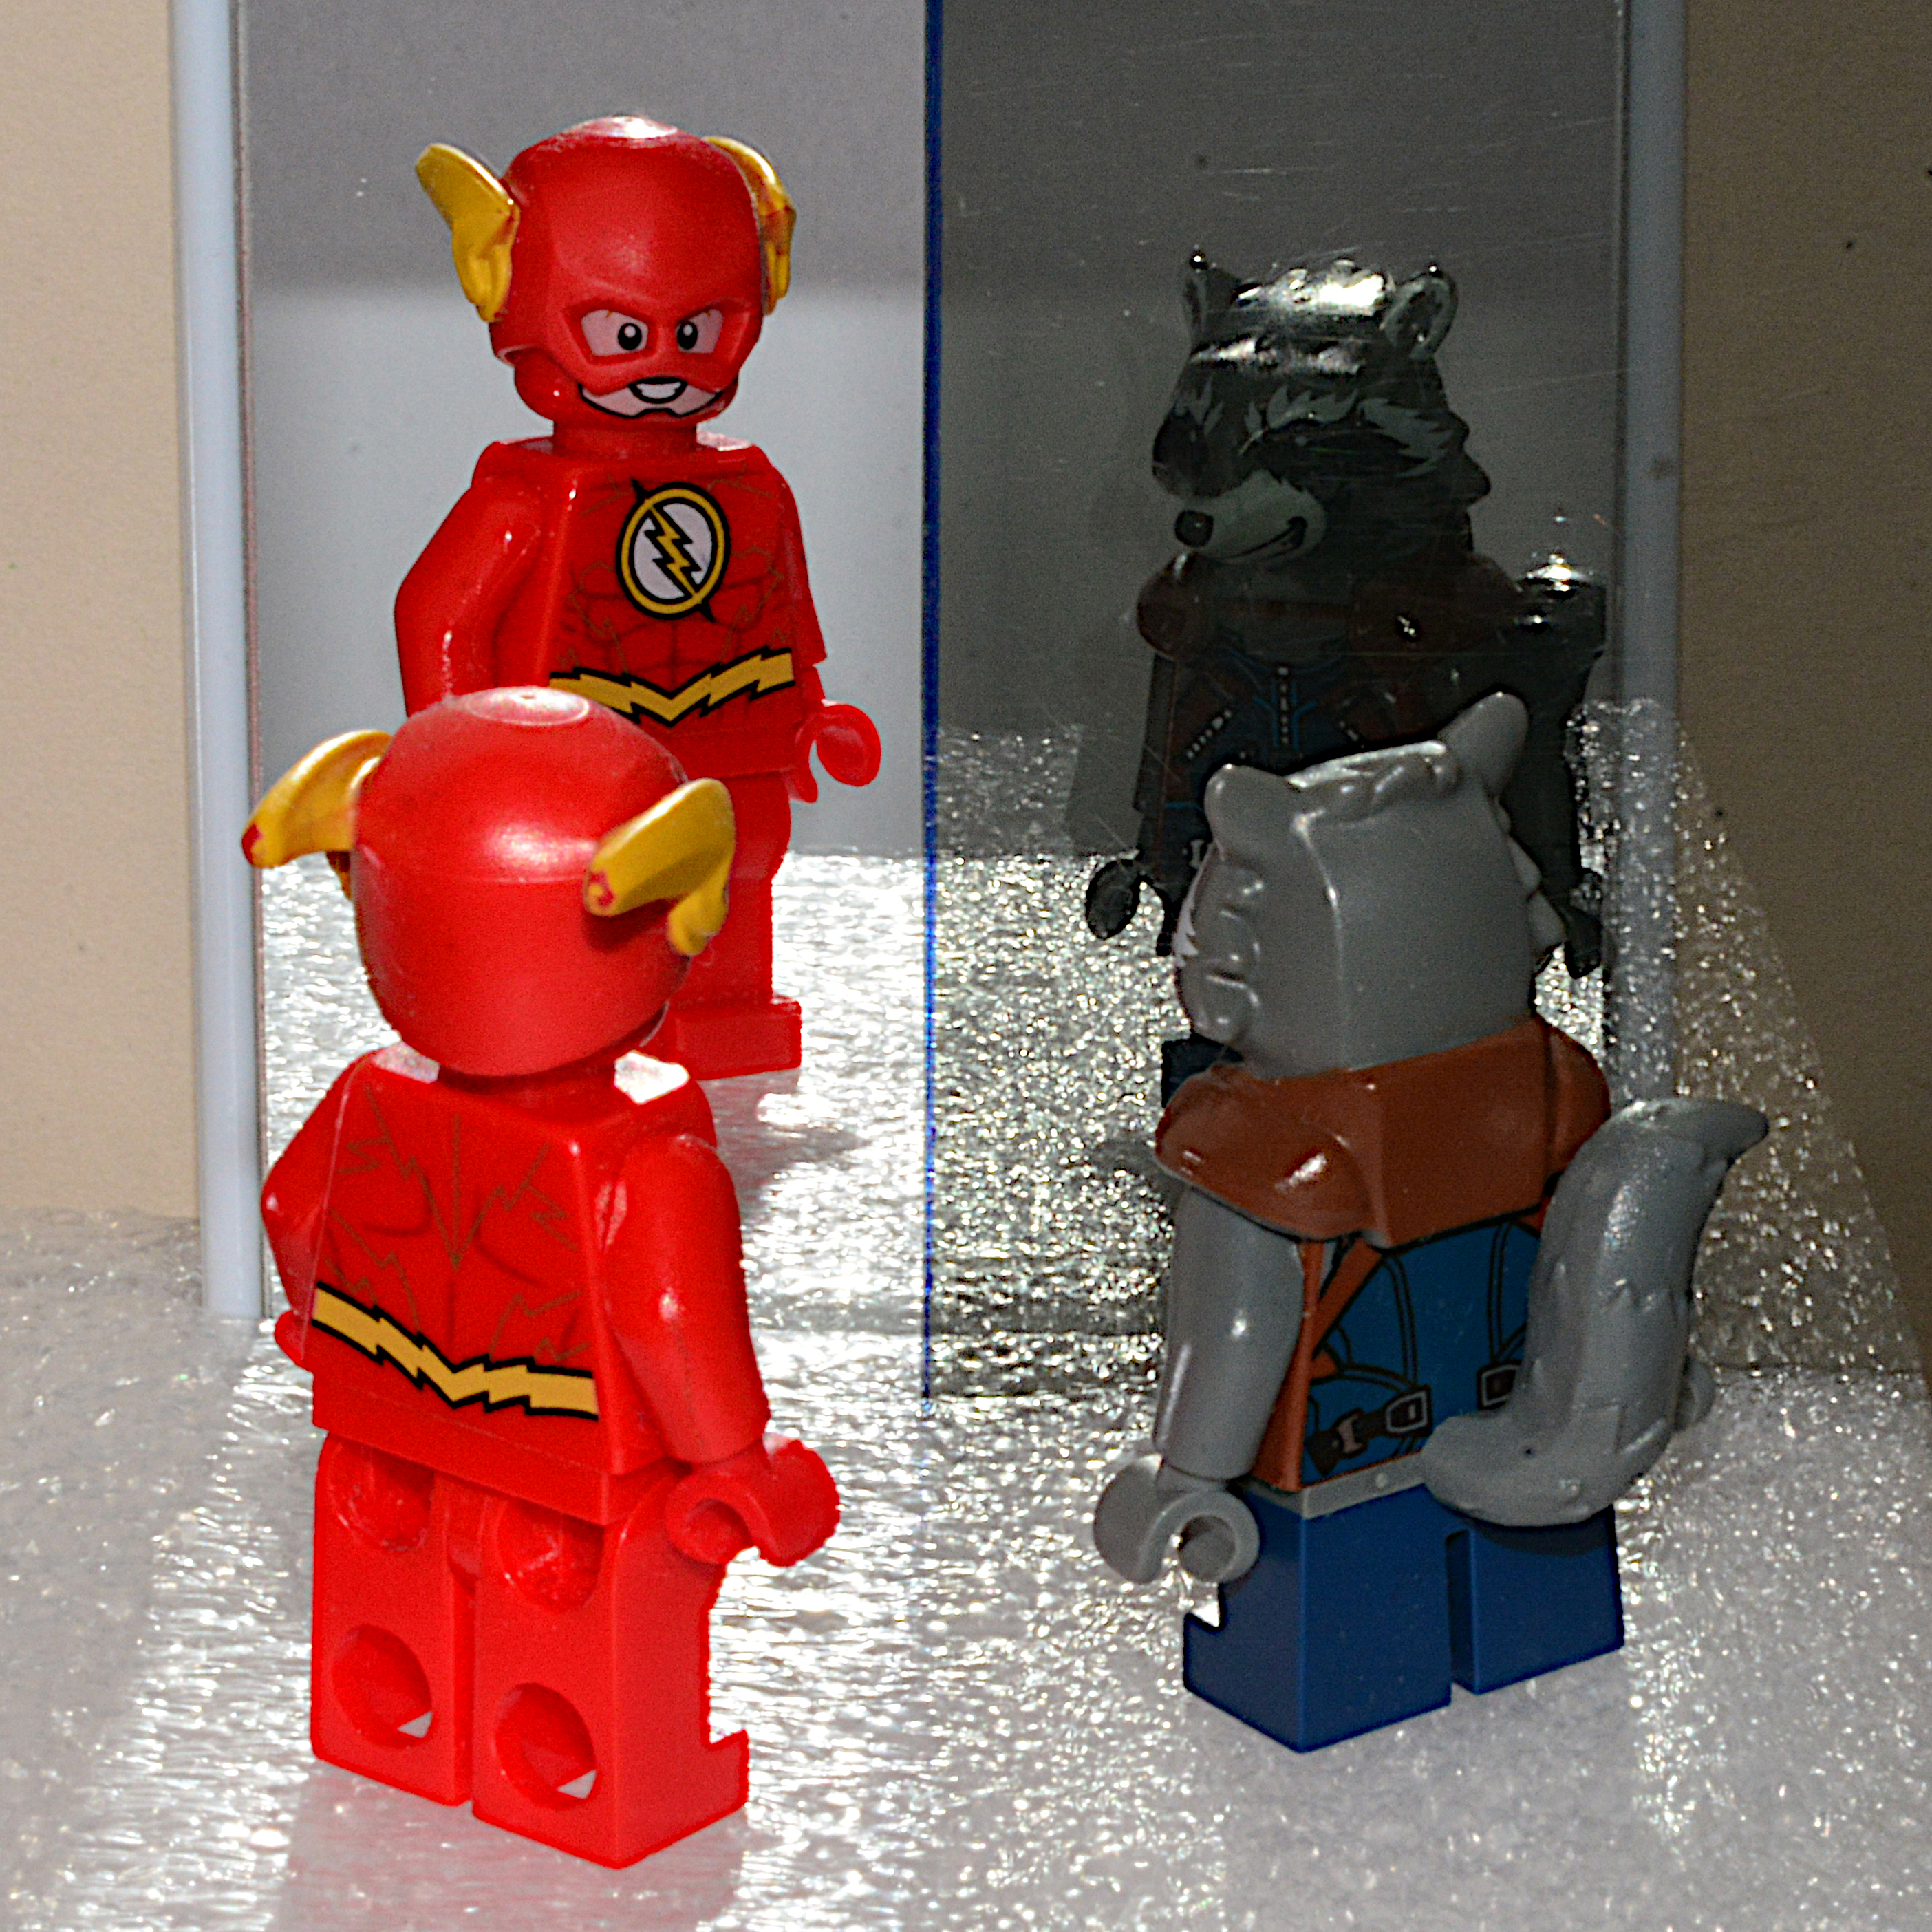
\includegraphics[width=7truecm]{slike/03_linodboj.JPG}\hfill
\includegraphics[width=7truecm]{slike/03_circodboj.JPG}
\caption{Linearno polarizirano valovanje pri odboju in prehodu skozi linearni polarizator
vidimo (levo). Cirkularno polarizirano valovanje se pri odboju spremeni iz 
desno polariziranega v levo polarizirano in obratno, zato pri ponovnem 
prehodu skozi cirkularni polarizator slike ni (desno).}
\label{fig:03_CirkularniOdboj}
\end{figure}
\end{example}

\begin{example}{\bf Zamenjava optičnih elementov.}
Poglejmo še učinek vrstnega reda optičnih elementov. Izberimo
kombinacijo linearnega in cirkularnega polarizatorja. V enem primeru postavimo
linearni polarizator pred cirkularnega, v drugem pa za njega. Razlika
v prepuščeni svetlobi jasno kaže pomembnost vrstnega reda optičnih
elementov in seveda tudi vrstnega reda zapisa matrik.
\begin{figure}[h!]
\centering
\includegraphics[width=7truecm]{slike/03_vrstnired1.JPG}\hfill
\includegraphics[width=7truecm]{slike/03_vrstnired2.JPG}
\caption{Učinek vpliva vrstnega reda cirkularnega in linearnega polarizatorja.
Na levi sliki je spredaj linearni polarizator in za njim cirkularni, na desni sliki
je vrstni red obrnjen in svetloba je prepuščena.}
\label{fig:03_VrstniRed}
\end{figure}
\end{example}

\section{Valovna enačba v prevodni snovi}
\label{section:35}
Obravnavajmo za konec še valovno enačbo v prevodni snovi. Snov naj
bo homogena, izotropna in nenabita ($\varrho_e = 0$). Izhajamo\index{Valovna enačba!{v prevodniku}|see{Telegrafska enačba}}
iz Maxwellovih enačb (enačbe~\ref{eq:Maxwell1}--\ref{eq:Maxwell4}) in zveze:
\begin{equation}
\mathbf{j}_e = \sigma \mathbf{E},
\label{eq:03_65}
\end{equation}
ki povezuje gostoto električnega toka $\mathbf{j}_e $ in jakost 
električnega polja $\mathbf{E}$. Sorazmernostni faktor, ki predstavlja\index{Električna prevodnost}
električno prevodnost, smo označili s $\sigma$. Tipična vrednost
za kovine je $\sigma > 10^6/\si{\ohm\m}$ in za izolatorje 
$\sigma < 10^{-6}/\si{\ohm\m}$. 
Električne tokove moramo upoštevati pri zapisu Amp\`{e}rovega zakona 
(enačba~\ref{eq:Maxwell1}):
\begin{equation}
\nabla\times\mathbf{H} =\frac{\partial\mathbf{D}}{\partial t}+\mathbf{j}_e = 
\varepsilon \varepsilon_0 \frac{\partial\mathbf{E}}{\partial t}+\sigma \mathbf{E}.
\label{eq:03_66}
\end{equation}
Izhajamo iz Faradayevega zakona (enačba~\ref{eq:Maxwell2}) in na njem izvedemo operacijo rotorja:
\begin{equation}
\nabla \times \left( \nabla \times  \mathbf{E}\right) = -\nabla\times \left(
\frac{\partial \mathbf{B}}{\partial t}\right) = - \mu \mu_0 \frac{\partial }{\partial t}
\left( \nabla \times \mathbf{H}\right)\!\!.
\label{eq:03_67}
\end{equation}
Vstavimo enačbo~(\ref{eq:03_66}) in dobimo:
\begin{equation}
\nabla \times \left( \nabla \times  \mathbf{E}\right) =
 -\mu \mu_0 \frac{\partial }{\partial t}
\left( \varepsilon \varepsilon_0 \frac{\partial\mathbf{E}}{\partial t}\right)-
\mu \mu_0 \frac{\partial }{\partial t}\left(\sigma \mathbf{E} \right)\!\!.
\label{eq:03_671}
\end{equation}
Upoštevamo še enačbo~(\ref{eq:03_02}) in dobimo zvezo:
\boxeq{eq:telegrafska}{
\nabla^2\mathbf{E} =  \mu \mu_0\varepsilon \varepsilon_0 \frac{\partial^2\mathbf{E}}{\partial t^2}
+ \mu \mu_0 \sigma \frac{\partial \mathbf{E}}{\partial t}.
}
Zapisano enačbo imenujemo telegrafska enačba. Podobno izpeljemo tudi telegrafsko enačbo
za gostoto magnetnega polja $\mathbf{B}$.\index{Telegrafska enačba}

Ker v telegrafski enačbi nastopa prvi odvod po času, po analogiji z mehanskimi
sistemi pričakujemo, da se valovanje v snovi duši oziroma slabi (atenuira). 
Rešitev zato iščemo v obliki ravnega valovanja:
\begin{equation}
\mathbf{E}(\mathbf{r},t) = \mathbf{E}_0 e^{i\mathbf{k}\cdot \mathbf{r} - i\omega t},
\label{eq:03_68}
\end{equation}
pri čemer dopuščamo možnost kompleksnega valovnega vektorja,\index{Valovni vektor!kompleksni} katerega imaginarni del
bo opisoval pojemanje amplitude. Ko nastavek (enačba~\ref{eq:03_68})
vstavimo v telegrafsko enačbo (enačba~\ref{eq:telegrafska}), dobimo:
\begin{equation}
-k^2 \mathbf{E} = \mu \mu_0\varepsilon \varepsilon_0 \left (-\omega^2 \mathbf{E}\right)
+ \mu \mu_0 \sigma \left(-i \omega\right)\mathbf{E}.
\label{eq:03_69}
\end{equation}
Sledi:
\begin{equation}
k^2 = \mu \mu_0\varepsilon \varepsilon_0 \omega^2 + i \mu \mu_0 \sigma\omega = 
\frac{\omega^2}{c_0^2} \varepsilon \mu  + i \frac{\omega^2}{c_0^2}\frac{\sigma \mu}{\varepsilon_0\omega}.
\label{eq:03_70}
\end{equation}
Vstavimo valovno število v vakuumu $k_0 = \omega/c_0$ in dobimo:
\begin{equation}
k^2 = k_0^2 \left( \varepsilon \mu + i \frac{\sigma \mu}{\varepsilon_0\omega} 
\right)\!\!.
\label{eq:03_71}
\end{equation}
Vpeljemo kompleksni lomni količnik $\mathcal{N}$, tako da velja:\index{Lomni količnik!kompleksni}
\boxeq{eq:nkompleks}{
k = k_0 \mathcal{N}.
}
Pri tem je:
\boxeq{eq:nkompleks2}{
\mathcal{N}^2 = \varepsilon \mu + i \frac{\sigma \mu}{\varepsilon_0\omega}.
}
Kompleksni lomni količnik $\mathcal{N}$ zapišemo kot vsoto realnega $n'$ in imaginarnega
dela $n''$:
\begin{equation}
\mathcal{N}^2 = (n'+in'')^2 = n'^2 -n''^2 + 2i n'n''.
\label{eq:03_72}
\end{equation}
Označimo realni del $\mathcal{N}^2$ (enačba~\ref{eq:nkompleks2})
z $x = \varepsilon \mu$ in imaginarni del z $y = \sigma \mu/\varepsilon_0\omega$.  
Rešujemo torej enačbo:
\begin{equation}
x + iy = n'^2 -n''^2 + 2i n'n''.
\label{eq:03_72a}
\end{equation}
Ločimo realni del:
\begin{equation}
x = n'^2 -n''^2
\label{eq:03_73}
\end{equation}
in imaginarni del:
\begin{equation}
y = 2n'n''.
\label{eq:03_74}
\end{equation}
Izrazimo $n''$ iz druge enačbe in ga vstavimo v prvo. Dobimo kvadratno enačbo:
\begin{equation}
n'^2-(y/2n')^2 = x
\label{eq:03_75}
\end{equation}
z rešitvijo:
\begin{equation}
n'^2 = \left(x + \sqrt{x^2+y^2}\right)/2.
\label{eq:03_76}
\end{equation}
Pri tem smo se omejili na rešitev s pozitivnim predznakom, saj je negativen predznak
za navadne snovi nesmiseln. Iz enačbe~(\ref{eq:03_73}) izračunamo še imaginarni del, 
ki je enak:
\begin{equation}
n''^2 = \left(-x + \sqrt{x^2+y^2}\right)/2.
\label{eq:03_77}
\end{equation}
Vstavimo izraza za $x$ in $y$ in dobimo:
\begin{equation}
n'^2 = \frac{1}{2}\left(\varepsilon \mu + \sqrt{(\varepsilon \mu)^2 + 
\left(\frac{\sigma \mu}{\varepsilon_0\omega}\right)^2}\right)
\label{eq:03_78}
\end{equation}
in
\begin{equation}
n''^2 = \frac{1}{2}\left(-\varepsilon \mu + \sqrt{(\varepsilon \mu)^2 + 
\left(\frac{\sigma \mu}{\varepsilon_0\omega}\right)^2}\right)\!\!.
\label{eq:03_79}
\end{equation}
Pogosto nas zanimajo nemagnetne snovi, v katerih je $\mu=1$. V takih
snoveh se kvadrat realnega dela lomnega količnika poenostavi v :
\begin{equation}
n'^2 = \frac{1}{2}\left(\varepsilon + \sqrt{\varepsilon^2 + 
\left(\frac{\sigma}{\varepsilon_0\omega}\right)^2}\right)\!\!,
\label{eq:03_80}
\end{equation}
kvadrat imaginarnega dela pa v:
\begin{equation}
n''^2 = \frac{1}{2}\left(-\varepsilon + \sqrt{\varepsilon^2 + 
\left(\frac{\sigma}{\varepsilon_0\omega}\right)^2}\right)\!\!.
\label{eq:03_81}
\end{equation}
Vstavimo zdaj izračunani lomni količnik v nastavek za jakost električnega polja 
(enačba~\ref{eq:03_68}) in poglejmo
primer, ko se svetloba širi v smeri $z$. Dobimo:
\begin{equation}
\mathbf{E} = \mathbf{E}_0 e^{ik_0\mathcal{N}z - i\omega t} = 
\mathbf{E}_0 e^{ik_0 n'z - i\omega t} \cdot e^{-k_0n''z}.
\label{eq:03_82}
\end{equation}
Zadnji člen opisuje eksponentno pojemanje amplitude polja z globino $z$ in ga pogosto
pišemo kot $\exp(-\kappa z)$, pri čemer je $\kappa = k_0 n''$.

V kovinah je prevodnost zelo velika in velja:
\begin{equation}
\frac{\sigma}{\omega\varepsilon_0} \gg \varepsilon.
\label{eq:03_83}
\end{equation}
Potem lahko imaginarni del lomnega količnika zapišemo kot:
\begin{equation}
n'' \approx \sqrt{\frac{\sigma}{2 \omega \varepsilon_0}}.
\label{eq:03_84}
\end{equation}
Parameter $\kappa$ je:
\begin{equation}
\kappa = k_0 n'' = \frac{\omega}{c_0} \sqrt{\frac{\sigma}{2 \omega \varepsilon_0}} = \sqrt{\frac{\mu_0 \omega \sigma}{2}}.
\label{eq:03_85}
\end{equation}
Nazornejše je vpeljati vdorno globino:\index{Vdorna globina}
\begin{equation}
d = \kappa^{-1} = \sqrt{\frac{2}{\mu_0 \omega \sigma}},
\label{eq:03_86}
\end{equation}
ki predstavlja karakteristično globino pojemanja električne poljske jakosti.
V kovinah je zaradi velike prevodnosti vdorna globina zelo majhna. Večina elektromagnetnega
valovanja oziroma izmeničnega toka zato teče po površini prevodnih snovi. Ta pojav poznamo pod imenom
kožni pojav.

\begin{example}{\bf Vdorna globina v bakru.}
Specifična upornost bakra je $\xi = 0,017~\si{\ohm\,\milli\metre^2/\metre}$ in 
prevodnost $\sigma = 1/\xi = 58 \times 10^6/\si{\ohm\metre}$. 
Vdorna globina je odvisna od frekvence elektro\-mag\-net\-nega valovanja, 
zato izračunajmo nekaj primerov: 
\begin{center}
\begin{tabular}{|c|c|}
\hline
$\nu~[\si{Hz}]$ & $d~[\si{nm}]$\\ \hline
50 & $\approx 10~\si{mm}$\\ \hline
$10^6$ & $\approx 100~\si{\micro\metre}$\\ \hline
$10^{10}$ & $\approx 1~\si{\micro\metre}$\\ \hline
$10^{15}$ & $\approx 3~\si{\nano\metre}$\\ \hline
\end{tabular}
\end{center}

Vdorna globina za vidno svetlobo je v bakru torej nekaj nanometrov. 
Izredno kratka vdorna globina v kovinah predstavlja velik problem pri izdelavi prozornih elektrod, 
ki jih potrebujemo na primer za izdelavo sončnih celic
ali tekočekristalnih zaslonov. Zato za ta namen navadno uporabljamo
kovine z razmeroma majhno prevodnostjo (npr. indijev 
kositrov oksid, ITO) in veliko vdorno globino. Debelina plasti, ki
jo nanesemo na steklo in ki še prepušča večino vpadne svetlobe, je 
v takih kovinah razmeroma velika, tipično 
okoli $100~\si{nm}$. 
\end{example}

%\chapterimage{Geometrijska.jpg} % Chapter heading image

\chapter{Odboj in lom}
Dva izmed najosnovnejših optičnih pojavov sta odboj in lom valovanja, ki vpada na mejo
dveh sredstev. V tem poglavju bomo podrobneje spoznali, kako se svetloba odbije in lomi ter
kako se pri tem spremenita amplituda in faza valovanja. Opisali bomo totalni odboj,
vpeljali Brewstrov kot in na koncu na hitro spoznali še odboj svetlobe na meji s kovino.

\section{Robni pogoji na meji dveh dielektrikov}
Že geometrijska optika pove, kako se svetloba na meji dveh sredstev odbija 
in lomi. Vemo, da je odbojni kot enak vpadnemu (enačba~\ref{eq:odbojnizakon}), 
smer lomljenega žarka pa je odvisna od lomnih količnikov snovi (enačba~\ref{eq:lomnizakon}). 
Vendar geometrijska optika ne pove ničesar o amplitudah in fazah odbitega 
in prepuščenega vala. Za to potrebujemo valovno obravnavo svetlobe. 

Izhajamo iz Maxwellovih enačb (enačbe~\ref{eq:Maxwell1}--\ref{eq:Maxwell4}), ki 
opisujejo elektromagnetno valovanje v snovi. Za obravnavo prehoda
skozi mejo dveh snovi potrebujemo še ustrezne robne pogoje. Zapišimo jih
za mejo med snovema z lomnima količnikoma
$n_1$ in $n_2$. Na meji naj ne bo električnih tokov ali površinskih nabojev. 
V prvi snovi naj bo gostota električnega polja enaka $\mathbf{D}_1$, v drugi 
pa $\mathbf{D}_2$.

Zapišimo Gaussov zakon (enačba~\ref{eq:Maxwell3}) v integralni obliki:
\beq
\oint \mathbf{D}\cdot d\mathbf{S} = 0.
\label{eq:04_01}
\eeq
\begin{figure}[ht]
\centering
\def\svgwidth{120truemm} 
\input{slike/04_RP.pdf_tex}
\caption{K izpeljavi robnih pogojev na meji dveh snovi. Prvi robni pogoj je ohranitev
pravokotne komponente $\mathbf{D}$ (a), drugi pa ohranitev tangentne komponente 
$\mathbf{E}$ (b).}
\label{fig:04_RP}
\end{figure}

Sklenjena ploskev, po kateri integriramo, naj bo kvader z dvema stranicama
vzporednima mejni ploskvi (slika~\ref{fig:04_RP}\,a). 
Ko gre višina kvadra $h \to 0$, ostaneta le še dva prispevka k integralu:
\beq
\mathbf{D}_1 \cdot \mathbf{s}_0 + \mathbf{D}_2 \cdot (-\mathbf{s}_0) = 0,
\label{eq:04_02}
\eeq
pri čemer vektor $\mathbf{s}_0 $ opisuje normalo na ploskev kvadra in hkrati
tudi normalo na mejno ravnino. Sledi:
\boxeq{eq:RPD}{
\left( \mathbf{D}_2-\mathbf{D}_1 \right) \cdot \mathbf{s}_0 = 0 \qquad \mathrm{oziroma} \qquad
D_{1\perp} = D_{2\perp}.
}
Pri prehodu skozi mejo dveh snovi se torej ohranja normalna komponenta gostote
električnega polja. Povsem enak račun lahko naredimo za gostoto magnetnega polja, 
če izhajamo iz enačbe:
\beq
\oint \mathbf{B}\cdot d\mathbf{S} = 0.
\label{eq:04_03}
\eeq
Pri prehodu skozi mejo dveh snovi se tako ohranja normalna komponeneta
gostote magnetnega polja:
\boxeq{eq:RPB}{
\left( \mathbf{B}_2-\mathbf{B}_1 \right) \cdot \mathbf{s}_0 = 0 \qquad 
\mathrm{oziroma} \qquad B_{1\perp} = B_{2\perp}.
}

Naredimo zdaj še pravokotno zanko, ki leži v ravnini, pravokotni na mejo dveh 
sredstev (slika~\ref{fig:04_RP}\,b). Zanko 
lahko vedno izberemo tako, da leži v ravnini, ki jo tvorita vektorja normale na 
mejo $\mathbf{s}_0$ in jakosti električnega polja $\mathbf{E}$. 
Zapišemo Faradayev zakon (enačba~\ref{eq:Maxwell2}) v integralni obliki, pri 
čemer integriramo po sklenjeni zanki:
\beq
\oint \mathbf{E}\cdot d\mathbf{l} = - \frac{\partial}{\partial t}\int \mathbf{B}\cdot d\mathbf{S}.
\label{eq:04_04}
\eeq
Višino zanke naredimo kar se da majhno ($h \to 0$), zato ostaneta le še 
integrala po zgornji in spodnji stranici:
\beq
\mathbf{E}_1 \cdot d\mathbf{l} - \mathbf{E}_2 \cdot d\mathbf{l} = 0.
\label{eq:04_05}
\eeq
Ohranja se torej projekcija vektorja jakosti električnega polja na mejo. 
Ker je vektor $d\mathbf{l}$ vzporeden z mejo, vektor $d\mathbf{s}_0$ pa 
pravokoten nanjo, lahko zgornji izraz zapišemo kot:
\boxeq{eq:RPE}{
\left( \mathbf{E}_2-\mathbf{E}_1 \right) \times \mathbf{s}_0 = 0 \qquad \mathrm{oziroma} \qquad
E_{1 \parallel} = E_{2 \parallel}.
}
Podobno izpeljemo tudi robni pogoj za ohranitev tangentne komponente
jakosti magnetnega polja:
\boxeq{eq:RPH}{
\left( \mathbf{H}_2-\mathbf{H}_1 \right) \times \mathbf{s}_0 = 0 \qquad \mathrm{oziroma} \qquad
H_{1\parallel} = H_{2\parallel}.
}

\section{Odbojni in lomni zakon}
Zamislimo si ravno potujoče sinusno elektromagnetno valovanje, ki vpada na mejo dveh snovi
z lomnima količnikoma $n_1$ in $n_2$. Vemo, da se vpadno valovanje razdeli na odbito in prepuščeno (lomljeno) valovanje. Zanima nas, kakšne lastnosti morata imeti odbito in prepuščeno valovanje, da zadostita robnim pogojem. 
\begin{figure}[ht]
\centering
\def\svgwidth{120truemm} 
\input{slike/04_lom.pdf_tex}
\caption{K izpeljavi odboja in loma na meji dveh snovi (a). Pri odboju in lomu
se ohranja komponenta valovnega vektorja, ki je vzporedna z mejno ploskvijo (b).}
\label{fig:04_lom}
\end{figure}

Naj žarek svetlobe vpada na mejno ravnino pod kotom $\alpha$ glede na normalo na mejo (glej
sliko~\ref{fig:04_lom}). Njegov valovni vektor naj bo $\mathbf{k}_i$, 
krožna frekvenca $\omega_i$, faza $\delta_i$ in amplituda $\mathbf{E}_{0i}$. 
Pripadajoče valovno število
je $k_i = \omega_i n_1/c_0$. Vpadni val na splošno zapišemo kot:
\beq
\mathbf{E}_i = \mathbf{E}_{0i} e^{i\mathbf{k}_i\cdot \mathbf{r} - i \omega_i t + i \delta_i}.
\label{eq:04_06}
\eeq
Podobno zapišemo odbiti val z valovnim vektorjem $\mathbf{k}_r$, 
krožno frekvenco $\omega_r$, fazo $\delta_r$ in amplitudo $\mathbf{E}_{0r}$: 
\beq
\mathbf{E}_r = \mathbf{E}_{0r} e^{i\mathbf{k}_r\cdot \mathbf{r} - i \omega_r t + i \delta_r}
\label{eq:04_07}
\eeq
in prepuščeni val z valovnim vektorjem $\mathbf{k}_t$, 
krožno frekvenco $\omega_t$, fazo $\delta_t$ in amplitudo $\mathbf{E}_{0t}$:
\beq
\mathbf{E}_t = \mathbf{E}_{0t} e^{i\mathbf{k}_t\cdot \mathbf{r} - i \omega_i t + i \delta_t}.
\label{eq:04_08}
\eeq
Mejo med snovema postavimo v ravnino $z=0$. Iz robnega pogoja za ohranitev tangentne
komponente vektorja $\mathbf{E}$ (enačba~\ref{eq:RPE}) dobimo zvezo:
\beq
\mathbf{E}_{i\parallel} + \mathbf{E}_{r\parallel} = \mathbf{E}_{t\parallel},
\label{eq:04_09}
\eeq
oziroma izpisano:
\beq
\mathbf{E}_{0i\parallel} e^{ik_{ix}x+ik_{iy}y - i \omega_i t + i \delta_i}+
\mathbf{E}_{0r\parallel} e^{ik_{rx}x+ik_{ry}y - i \omega_r t + i \delta_r} =
\mathbf{E}_{0t\parallel} e^{ik_{tx}x+ik_{ty}y - i \omega_i t + i \delta_t}.
\label{eq:04_10}
\eeq
Pri tem smo upoštevali $z=0$. Zapisana zveza mora veljati 
ob vseh časih $t$ in za vse vrednosti $x$ in $y$. Vzemimo najprej $x=y=0$ in $t=0$. 
Od tod sledi, da so vse fazne enake in $\delta_i = \delta_r = \delta_t$.
Drugi pogoj poglejmo pri $x=y=0$ in poljubnem času $t>0$. Robni pogoj 
je izpolnjen le v primeru, da velja 
\boxeq{eq:omegakonst}{
\omega_i =
\omega_r = \omega_t
}
in se torej frekvenca pri odboju in lomu ohranja. 

Obravnavajmo zdaj primer $t=0$ pri poljubnem paru $x,y$ oziroma vektorju $\mathbf{r}$
v mejni ravnini. Da bo lahko robni pogoj izpolnjen za vsak $\mathbf{r}$,
mora veljati:
\beq
\mathbf{k}_i\cdot \mathbf{r} = \mathbf{k}_r\cdot \mathbf{r} = \mathbf{k}_t\cdot \mathbf{r} = \mathrm{konst.}
\label{eq:04_11}
\eeq
Iz tega sledi, da so projekcije vseh treh valovnih vektorjev na mejno
ravnino enake. Pomembnejša je ugotovitev, da ležijo valovni vektorji vpadnega, odbitega
in lomljenega valovanja vedno v eni ravnini. Imenujemo jo vpadna ravnina. 

Navadno izberemo, da je vpadna ravnina ravnina $xz$. Potem zapišemo 
valovne vektorje vpadne, odbite in prepuščene svetobe kot:
\begin{align}
\mathbf{k}_i  =& \left( \sin\alpha, 0, \cos \alpha\right) \frac{\omega}{c_0} n_1, \label{eq:04_12}\\
\mathbf{k}_r  =& \left( \sin\tilde{\alpha}, 0, -\cos \tilde{\alpha}\right) \frac{\omega}{c_0} n_1,\label{eq:04_13}\\
\mathbf{k}_t  =& \left( \sin\beta, 0, \cos \beta\right) \frac{\omega}{c_0} n_2.\label{eq:04_14}
\end{align}
Pri tem smo poleg vpadnega kota $\alpha$ vpeljali še odbojni kot $\alpha'$ in lomni
kot $\beta$. Iz enačbe~(\ref{eq:04_11}) neposredno sledi, da se mora ohranjati komponenta
valovnega vektorja, ki je vzporedna z mejno ravnino:
\beq
k_{ix} = k_{rx} = k_{tx}.
\label{eq:04_15}
\eeq
Najprej poglejmo prvo enakost ($k_{ix} = k_{rx}$). Vstavimo komponenti valovnih
vektorjev (enačbi~\ref{eq:04_12} in \ref{eq:04_13}) in dobimo:
\beq
\frac{\omega}{c_0} n_1 \sin \alpha  =  \frac{\omega}{c_0} n_1 \sin\tilde{\alpha},
\label{eq:04_16}
\eeq
od koder sledi odbojni zakon, ki pravi, da je odbojni kot enak vpadnemu:
\boxeq{eq:odbojni}{
\tilde\alpha = \alpha.
}

Poglejmo zdaj še drugo enakost ($k_{ix} = k_{tx}$). Vstavimo komponenti
valovnih vektorjev (enačbi~\ref{eq:04_12} in \ref{eq:04_14}) in dobimo:
\beq
\frac{\omega}{c_0} n_1 \sin \alpha  = \frac{\omega}{c_0} n_2\sin\beta.
\label{eq:04_17}
\eeq
Od tu sledi lomni zakon:
\boxeq{eq:04_18}{
n_1 \sin \alpha = n_2 \sin \beta.
}

Z odbojnim in lomnim zakonom smo izpolnili ujemanje faz v enačbi~(\ref{eq:04_10}). 
Hribi in doline vpadnega, odbitega in prepuščenega valovanja vzdolž meje 
potujejo enako hitro. Dodatno informacijo o valovanju dobimo, če
uskladimo še amplitude jakosti električnih polj. Preden izpeljemo
zveze, ki povezujejo razmerja med amplitudami, vpeljimo koordinatni sistem
in se dogovorimo o oznaki polarizacij.

Za obravnavo izberemo dve ortogonalni linearni polarizaciji, saj lahko potem
poljubno polarizacijo sestavimo kot kombinacijo teh dveh.
Mejna ravnina naj bo kot do zdaj ravnina $xy$, os $z$ pa naj bo obrnjena navzdol. 
V prvem primeru naj bo jakost elektičnega polja
vpadne, odbite in prepuščene svetlobe vzporedna z osjo $y$ in tako pravokotna
na vpadno ravnino (slika~\ref{fig:04_tetm}\,a). 
Tako valovanje imenujemo transverzalno električno (TE) valovanje. 
V literaturi pogosto najdemo oznaki $s$ (kot {\it senkrecht}, pravokotno) ali $\sigma$.

\begin{figure}[ht]
\centering
\def\svgwidth{140truemm} 
\input{slike/04_tetm.pdf_tex}
\caption{V primeru transverzalne električne (TE) polarizacije leži jakost
električnega polja pravokotno na vpadno ravnino (a),
pri transverzalni magnetni (TM) polarizaciji pa leži jakost električnega
polja v vpadni ravnini (b).}
\label{fig:04_tetm}
\end{figure}

V drugem primeru ležijo jakosti električnega polja v 
vpadni ravnini (slika~\ref{fig:04_tetm}\,b), gostote magnetnega polja 
pa so pravokotne na njih. To polarizacijo zato poimenujemo 
transverzalna magnetna (TM) polarizacija. Uporabljajo se tudi oznake
$p$ (kot {\it parallel}, vzporedno) ali $\pi$. 
Omenjena primera bomo obravnavali ločeno, začenši s TE polarizacijo. V 
obeh primerih se bomo omejili na izotropne in nemagnetne snovi ($\mu=1$).

\section{Fresnelove enačbe za transverzalno električno valovanje}
Osnovna zahteva na meji dveh snovi je izpolnjevanje robnih
pogojev, po katerih se na meji ohranja tangentna komponenta jakosti električnega
polja. Ker so vse tri jakosti vzporedne z osjo $y$, velja preprosta zveza:
\beq
E_{0i} + E_{0r}= E_{0t}
\label{eq:04_19}
\eeq
Pri tem smo upoštevali, da je polje v prvi snovi superpozicija vpadnega in odbitega
polja, v drugi snovi pa je samo prepuščeno valovanje. Drugi robni pogoj, ki zahteva
ohranitev normalne komponente gostote električnega polja (enačba~\ref{eq:RPD}) je 
vedno izpolnjen, saj je ta komponenta v obeh snoveh identično enaka nič. 
Tretji robni pogoj (enačba~\ref{eq:RPH}) zahteva
ohranitev tangentne komponente jakosti magnetnega polja. Privzamemo, da
sta snovi nemagnetni $\mu=1$ in dobimo:
\beq
-B_{0i}\cos \alpha + B_{0r}\cos \alpha = -B_{0t}\cos \beta.
\label{eq:04_20}
\eeq
Upoštevajoč zvezo med amplitudama električnega in magnetnega 
polja $E_0 = B_0 c = B_0 c_0/n$  (enačba~\ref{eq:EBc}) zapišemo robni pogoj kot:
\beq
-E_{0i}n_1\cos \alpha + E_{0r}n_1\cos \alpha = -E_{0t}n_2\cos \beta,
\label{eq:04_21}
\eeq 
oziroma:
\beq
n_1 E_{0i} \cos \alpha  -n_1 E_{0r}\cos \alpha = n_2 E_{0t}\cos \beta.
\label{eq:04_22}
\eeq
Na koncu zapišemo še četrti robni pogoj, ohranitev normalne komponente
gostote magnetnega polja (enačba~\ref{eq:RPB}):
\beq
B_{0i} \sin \alpha  + B_{0r}\sin \alpha = B_{0t}\sin \beta.
\label{eq:04_23}
\eeq
Ponovno uporabimo zvezo med amplitudami (enačba~\ref{eq:EBc}) in dobimo:
\beq
n_1  \sin \alpha \left( E_{0i} + E_{0r} \right) = n_2 E_{0t} \sin \beta.
\label{eq:04_24}
\eeq
Upoštevamo še lomni zakon (enačba~\ref{eq:04_18}) in dobimo:
\beq
E_{0i} + E_{0r} = E_{0t}.
\label{eq:04_25}
\eeq
Ta pogoj je ekvivalenten prvemu pogoju (enačba~\ref{eq:04_19}). Iz robnih
pogojev tako dobimo dve neodvisni enačbi (enačbi~\ref{eq:04_19} in \ref{eq:04_22}) 
za tri neznake: $E_{0i}$, $E_{0r}$ in $E_{0t}$. Navadno izrazimo amplitudi
odbitega in prepuščenega valovanja z amplitudo vpadnega valovanja in tako določimo 
relativno amplitudo odbite in prepuščene svetlobe. Izračunajmo ju.

Najprej pomnožimo enačbo~(\ref{eq:04_19}) z $n_2 \cos \beta$ in od nje odštejemo
enačbo~(\ref{eq:04_22}). Dobimo:
\beq
\left( n_2 \cos \beta-n_1 \cos \alpha\right) E_{0i} + 
\left( n_2 \cos \beta+n_1 \cos \alpha\right) E_{0r} = 0.
\label{eq:04_26}
\eeq
Vpeljemo amplitudno odbojnost $r = E_{0r}/E_{0i}$ 
kot razmerje odbite in vpadne amplitude valovanja. Iz enačbe~(\ref{eq:04_26}) sledi:
\boxeq{eq:TEr}{
r  = \frac{n_1 \cos \alpha - n_2 \cos \beta}
{n_1 \cos \alpha + n_2 \cos \beta},
}
pri čemer $\alpha$ in $\beta$ označujeta vpadni in lomni kot. Izraz za $r$
lahko z porabo lomnega zakona preoblikujemo:
\beq
r = \frac{\frac{n_1}{n_2} \cos \alpha - \cos \beta}{\frac{n_1}{n_2} \cos \alpha - \cos \beta} = 
\frac{\frac{\sin \beta}{\sin \alpha} \cos \alpha - \cos \beta}
{\frac{\sin \beta}{\sin \alpha} \cos \alpha - \cos \beta} = \frac{\sin \beta \cos \alpha -
\cos \beta \sin \alpha}{\sin \beta \cos \alpha + \cos \beta \sin \alpha} = 
-\frac{\sin (\alpha -\beta)}{\sin (\alpha + \beta)}.
\label{eq:04_27}
\eeq

Izračunajmo še amplitudno prepustnost $t = E_{0t}/E_{0i}$, ki jo vpeljemo
kot razmerje amplitud prepuščenega in vpadnega valovanja. Izhajamo
iz prvega robnega pogoja (enačba~\ref{eq:04_19}) in zapišemo:
\beq
t = \frac{E_{0t}}{E_{0i}} = \frac{E_{0i} + E_{0r}}{E_{0i}} = 1+ r.
\label{eq:04_28}
\eeq
Amplitudna prepustnost je tako:
\boxeq{eq:TEt}{
t = 1+r = \frac{2n_1\cos \alpha}{n_1 \cos \alpha + n_2 \cos \beta}.
}

\section{Fresnelove enačbe za transverzalno magnetno valovanje}
Izračunajmo še amplitudno odbdojnost in prepustnost za 
transverzalno magnetno polarizirano valovanje. Tudi v tem primeru začnemo
z robnimi pogoji. Na meji dveh sredstev se ohranja tangentna 
komponenta jakosti magnetnega polja (enačba~\ref{eq:RPH}):
\beq
H_{0i} + H_{0r}= H_{0t}.
\label{eq:04_29}
\eeq
Privzamemo, da so snovi nemagnetne in velja: $\mu_1 = \mu_2 = 1$. Potem enačbo
prepišemo v:
\beq
B_{0i} + B_{0r}= B_{0t}.
\label{eq:04_30}
\eeq
Iz zveze med amplitudama električnega in magnetnega polja (enačba~\ref{eq:EBc})
dobimo:
\beq
E_{0i}n_1 + E_{0r}n_1= E_{0t}n_2.
\label{eq:04_31}
\eeq
Drugi robni pogoj (enačba~\ref{eq:RPB}), ki pravi, da se ob prehodu v drugo snov ohranja
pravokotna komponenta gostote magnetnega polja, je prav tako izpolnjen, saj je $B_{\perp}=0$. 
Iz tretjega robnega pogoja, ohranitve tangentne komponente jakosti
električnega polja (enačba~\ref{eq:RPE}), sledi:
\beq
E_{0i} \cos \alpha - E_{0r}\cos \alpha = E_{0t}\cos \beta.
\label{eq:04_32}
\eeq
Predznak jakosti električnega polja smo zapisali v skladu s sliko~\ref{fig:04_tetm}. 
Za vajo lahko zapišemo še četrti robni pogoj, ki pomeni ohranitev normalne 
komponenete gostote električnega polja $D_\perp$ (enačba~\ref{eq:RPD}):
\beq
D_{0i}\sin \alpha - D_{0r}\sin \alpha = D_{0t}\sin \beta.
\label{eq:04_33}
\eeq
Upoštevamo, da je $D_0 = \varepsilon \varepsilon_0 E_0 = \varepsilon_0 n^2 E_0$ in
zapišemo:
\beq
E_{0i} n_1^2 \sin \alpha - E_{0r} n_1^2 \sin \alpha  = 
E_{0t} n_2^2 \sin \beta = E_{0t} n_1 n_2 \sin \alpha.
\label{eq:04_34}
\eeq
Pri tem smo upoštevali lomni zakon. Po krajšanju dobimo enačbo, 
ki je enaka prvemu robnemu pogoju in ne da nove informacije. 
Ostaneta dve enačbi za tri neznanke in ponovno lahko
izrazimo amplitudi odbite in prepuščene svetlobe z amplitudo vpadne. 
Enačbo (\ref{eq:04_31}) pomnožimo s $\cos \beta$, enačbo~(\ref{eq:04_32}) pa z $n_2$:
\begin{align}
E_{0i} n_1 \cos \beta + E_{0r} n_1 \cos \beta  =& E_{0t} n_2 \cos \beta \label{eq:04_35} \\
E_{0i} n_2 \cos \alpha - E_{0r} n_2 \cos \alpha  =& E_{0t} n_2 \cos \beta\label{eq:04_36}.
\end{align}
Enačbi odštejemo in dobimo:
\beq
E_{0i} \left(n_1 \cos \beta - n_2 \cos \alpha \right) + E_{0r} \left(n_1 \cos \beta + 
n_2 \cos \alpha \right) = 0.
\label{eq:04_37}
\eeq
Od tod izračunamo amplitudno odbojnost $r = E_{0r}/E_{0i}$, ki je 
razmerje med odbito in vpadno amplitudo jakosti električnega polja:
\boxeq{eq:TMr}{
r = \frac{n_2 \cos \alpha - n_1 \cos \beta}{n_2 \cos \alpha + n_1 \cos \beta}.
}
Tudi ta izraz lahko predelamo z upoštevanjem lomnega zakona:
\beq
r = \frac{\frac{n_2}{n_1} \cos \alpha - \cos \beta}{\frac{n_2}{n_1} \cos \alpha - \cos \beta} = 
\frac{\frac{\sin \alpha}{\sin \beta} \cos \alpha - \cos \beta}
{\frac{\sin \alpha}{\sin \beta} \cos \alpha - \cos \beta} = 
\frac{\sin \alpha \cos \alpha -\cos \beta \sin \beta}
{\sin \alpha \cos \alpha + \cos \beta \sin \beta}.
\label{eq:04_38}
\eeq
To lahko zapišemo z dvojnimi koti:
\beq
r = \frac{\sin(2\alpha) - \sin(2\beta)}{\sin(2\alpha) + \sin(2\beta)},
\label{eq:04_39}
\eeq
nato pa razliko in vsoto sinusov zapišemo kot produkt in dobimo:
\beq
r = \frac{2\cos(\alpha+\beta )\sin(\alpha-\beta )}
{2\sin(\alpha+\beta )\cos(\alpha-\beta )} = \frac{\tan(\alpha-\beta )}{\tan(\alpha+\beta )}.
\label{eq:04_40}
\eeq
Amplitudno prepustnost $t = E_{0t}/E_{0i}$ 
izračunamo iz enačbe~(\ref{eq:04_31}):
\boxeq{eq:TMt}{
t = \frac{n_1}{n_2}\left(1+r \right) = 
\frac{2 n_1 \cos \alpha}{n_2 \cos \alpha + n_1 \cos \beta}.
}

\begin{example}{\bf Amplitudni odbojnost in prepustnost pri pravokotnem vpadu.} 
Izračunali smo amplitudni odbojnosti $r$ in prepustnosti $t$ za obe med seboj 
pravokotni polarizaciji TE in TM. Poglejmo zdaj najpreprostejši primer, pri katerem
svetloba vpada pravokotno na mejo snovi. V tem primeru so vpadni, odbojni in 
lomni kot enaki in $\alpha = \tilde{\alpha} = \beta = 0$. Za TE polarizacijo dobimo:
\beq
r_{\mathrm{TE}} = \frac{n_1 -n_2}{n_1+n_2} \qquad \mathrm{in} \qquad
t_{\mathrm{TE}} = \frac{2n_1}{n_1+n_2},
\label{eq:04_42}
\eeq
za TM polarizacijo pa:
\beq
r_{\mathrm{TM}} = \frac{n_2 -n_1}{n_2+n_1} \qquad \mathrm{in} \qquad
t_{\mathrm{TM}} = \frac{2n_1}{n_1+n_2}.
\label{eq:04_43}
\eeq
Ker je vpad pravokoten, pričakujemo enaka rezultata za obe polarizaciji, saj 
polarizacij pri pravokotnem vpadu ne moremo ločiti med seboj. Rezultata za
prepuščeno svetlobo sta res enaka, za odbito svetlobo pa se razlikujeta za predznak.
Vzrok za to navidezno neenakost je v začetni izbiri smeri polarizacije 
pri odboju (glej sliko~\ref{fig:04_tetm}).
Odbojnost je z upoštevanjem privzete smeri tako enaka za obe polarizaciji 
-- kar je seveda pravilno.
\end{example}

\section{Energijski tok pri odboju in lomu}
V poskusih nas navadno zanima energijski tok valovanja. Gostoto energijskega
toka na splošno zapišemo kot (enačba~\ref{eq:j}):
\beq
j = \frac{1}{2} \varepsilon_0^2 E_0^2 c_0 n.
\label{eq:04_44}
\eeq
Odbojnost $\mathcal{R}$ vpeljemo kot razmerje med gostotama energijskih
tokov odbite in vpadne svetlobe:
\beq
\mathcal{R} = \frac{j_r}{j_i} = \frac{\frac{1}{2}\varepsilon_0 E_{0r}^2 c_0 n_1}
{\frac{1}{2}\varepsilon_0 E_{0i}^2 c_0 n_1} = \left(\frac{E_{0r}}{E_{0i}}\right)^2\!\!.
\label{eq:04_45}
\eeq
V razmerju jakosti električnega polja prepoznamo amplitudno odbojnost in zapišemo:
\boxeq{eq:TEMR}{
\mathcal{R} = |r|^2.
}
Ker odbita in vpadna svetloba potujeta po isti snovi, je odbojnost kar 
enaka kvadratu razmerja amplitud polj. 

Izračunajmo še prepustnost $\mathcal{T}$, ki je razmerje med gostotama svetlobnih
tokov prepuščene in vpadne svetlobe. Pri zapisu je treba biti pazljiv, saj je 
treba upoštevati projekcijo povprečnega Poyntingovega vektorja. Zato zapišemo: 
\beq
\mathcal{T} = \frac{j_t}{j_i} = \frac{\frac{1}{2}\varepsilon_0 E_{0t}^2 c_0 n_2}
{\frac{1}{2}\varepsilon_0 E_{0i}^2 c_0 n_1} \frac{\cos\beta}{\cos\alpha}= 
\left(\frac{E_{0t}}{E_{0i}}\right)^2 \frac{n_2\cos\beta}{n_1\cos\alpha}.
\label{eq:04_46}
\eeq
Prepustnost je torej enaka:
\boxeq{eq:TEMT}{
\mathcal{T} = |t|^2 \frac{n_2\cos\beta}{n_1\cos\alpha}.
}

Izračunajmo vsoto odbojnosti in prepustnosti na primeru TE polariziranega valovanja:
\begin{align}
\mathcal{R}+ \mathcal{T}=&
\left(\frac{n_1 \cos \alpha - n_2 \cos \beta}{n_1 \cos \alpha + n_2 \cos \beta}\right)^2+
\frac{4n_1n_2\cos \alpha \, \cos \beta}{\left(n_1 \cos \alpha + n_2 \cos \beta\right)^2}\\ =& 
\frac{n_1^2 \cos^2\alpha + n_2^2\cos^2\beta -2 n_1n_2 \cos \alpha \cos \beta + 
4n_1n_2\cos\alpha \cos \beta}{\left(n_1 \cos \alpha + n_2 \cos \beta\right)^2}\\ = &
\frac{n_1^2 \cos^2\alpha + n_2^2\cos^2\beta +2 n_1n_2 \cos \alpha \cos \beta}
{n_1^2 \cos^2\alpha + n_2^2\cos^2\beta +2 n_1n_2 
\cos \alpha \cos \beta} = 1.
\label{eq:04_47}
\end{align}
Če povzamemo:
\boxeq{eq:TEMRT}{
\mathcal{R}+\mathcal{T} = 1.
}
Rezultat je seveda pričakovan, saj opisuje ohranitev energije. Pogosto je najbolj
priročno izračunati odbojnost, nato pa z uporabo enačbe~(\ref{eq:TEMRT})
preprosto še prepustnost. 

Opozorimo še enkrat, da je pri izračunu prepustnosti treba upoštevati tudi 
spremembo lomnega količnika in kota širjenja svetlobe, zato:
\beq
|r|^2+ |t|^2 \neq 1.
\label{eq:04_48}
\eeq

\begin{example}{\bf Odbojnost pri pravokotnem vpadu na steklo.} 
Izračunajmo, kolikšna je odbojnost svetlobe, ki vpada pod pravim kotom iz zraka na
steklo z lomnim količnikom $n_2=1,5$. Uporabimo enačbi~(\ref{eq:TEr}) in (\ref{eq:TEMR})
in dobimo:
\beq
\mathcal{R} = \left(\frac{n_1-n_2}{n_1+n_2}\right)^2 \approx~4~\%.
\label{eq:04_49}
\eeq
Ob pravokotnem vpadu na steklo se $4~\%$ svetlobe odbije, ostala 
svetloba je prepuščena.
\end{example}

\section{Prehod v optično gostejšo snov}
Najprej si oglejmo prehajanje svetlobe iz snovi z manjšim lomnim
količnikom v snov z večjim lomni količnikom ($n_1<n_2$). To je na primer
primer odboja in loma pri vpadu svetlobe iz zraka v vodo ali steklo. 

Narišimo najprej amplitudno odbojnost in prepustnost za TE polarizacijo v odvisnosti
od vpadnega kota (slika~\ref{fig:04_redte}\,a). 
Iz enačbe~(\ref{eq:TEr}) sledi, da je amplitudna odbojnost $r_\mathrm{TE}$
za vse kote negativna. Njena velikost se zvezno spreminja od začetne vrednosti
pri pravokotnem vpadu do vrednosti $-1$, ko se vpadni kot približuje $90\si{\degree}$.
Negativni predznak pri kotu $\alpha =0$ pomeni, da se svetloba pri 
pravokotnem vpadu na optično gostejše sredstvo vedno odbije z nasprotno fazo, ne 
glede na njeno polarizacijo.
\begin{figure}[ht]
\centering
\def\svgwidth{140truemm} 
\input{slike/04_redte.pdf_tex}
\caption{nknl}
\label{fig:04_redte}
\end{figure}

Amplitudna prepustnost $t_\mathrm{TE}$, ki jo izračunamo kot $t=r+1$, je za vse
vpadne kote pozitivna in pojema od največje vrednosti pri pravokotnem vpadu
do vrednosti $0$, ko se vpadni kot približuje $90\si{\degree}$. 
Odbojnost $\mathcal{R}_\mathrm{TE}$, ki jo izračunamo kot kvadrat amplitudne odbojnosti,
je prikazana na sliki~\ref{fig:04_redte}\,b. Vrednost je po pričakovanju 
vedno pozitivna in narašča od neke začetne vrednosti pri pravokotnem
vpadu do vrednosti $1$, ko se vpadi kot približuje $90\si{\degree}$. Prepustnost
$\mathcal{R}_\mathrm{TE}$ izračunamo po enačbi $\mathcal{T} = 1 -\mathcal{R}$. 

Poglejmo še primer transverzalne magnetne polarizacije. Narišemo odvisnost
$r$ in $t$ od vpadnega kota (slika~\ref{fig:04_redtm}\,a). Zaradi začetne 
izbire smeri odbite jakosti električnega polja je predznak pri pravokotnem vpadu drugačen kot pri 
polarizaciji TE in je pozitiven. Z naraščajočim vpadnim kotom se amplitudna
odbojnost zmanjšuje in doseže vrednost $r=-1$ ko se vpadni kot
približuje $\alpha = 90\si{\degree}$. Vidimo, da pri nekem kotu zavzame  
vrednost $r = 0$. Pri tem kotu, imenujemo ga Brewstrov kot $\alpha_B$, 
je odbojnost za TM polarizacijo enaka nič. To ima pomembno in uporabno
posledico, da je celotno TM polarizirano valovanje pri Brewstrovem kotu prepuščeno. 
Ker amplitudna odbojnost pri Brewstrovem kotu zamenja predznak, se pri tem
kotu tudi spremeni faza odbite svetlobe. 
\begin{figure}[ht]
\centering
\def\svgwidth{140truemm} 
\input{slike/04_redtm.pdf_tex}
\caption{nknl}
\label{fig:04_redtm}
\end{figure}

Odbojnost in prepustnost TM polariziranega valovanja sta prikazani na 
sliki~\ref{fig:04_redtm}\,b. Odbojnost od začetne vrednosti pri $\alpha=0$
pojema z naraščajočim vpadnim kotom do vrednosti 0, ki jo doseže pri 
Brewstrovem vpadnem kotu $\alpha_B$. Nato odbojnost strmo naraste z naraščajočim vpadnim
kotom do vrednosti 1. Prepustnost je enaka $\mathcal{T} = 1- \mathcal{R}$.

\subsection*{Brewstrov kot}
Brewstrov kot smo vpeljali kot kot, pri katerem je odbojnost
TM polariziranega valovanja enaka nič. Poglejmo, pri katerem
vpadnem kotu se to zgodi. Amplitudna odbojnost $r$ je po enačbi~(\ref{eq:04_40})
enaka:
\beq
r = \frac{\tan(\alpha-\beta)}{\tan(\alpha+\beta)}.
\label{eq:04_50}
\eeq
Pri vrednosti $\alpha + \beta = \pi/2$ imenovalec v izrazu za $r$ 
naraste v neskončnost. Števec je vedno različen od nič, saj
sta po lomnem zakonu vpadni in lomljeni kot vedno različna. Posledično
je pri vrednosti $\alpha + \beta = \pi/2$ odbojnost enaka nič.
Ob tem pogoju lahko zapišemo $\cos \alpha = \sin \beta$. Iz lomnega 
zakona sledi:
\beq
n_1 \sin \alpha = n_2 \sin \beta = n_2 \cos \alpha.
\label{eq:04_51}
\eeq
Od tod seledi, da za Brewstrov kot velja:
\boxeq{eq:Brewstrovkot}{
\tan \alpha_B = \frac{n_2}{n_1}.
}
Pri prehodu zrak/steklo je $\alpha_B = 56,3\si{\degree}$ in na meji
steklo/zrak $\alpha_B = 33,6\si{\degree}$. 

Zaradi tega pojava je odbojnost za TM polarizirano valovanje pri
večjih vpadnih kotih dosti manjša kot za TE polarizirano valovanje. 
Kadar osvetljujemo mejno ploskev z nepolarizirano svetlobo, se 
pri kotu $\alpha_B$ od mejne ploskve odbije samo TE polarizirano
valovanje, TM pa je v celoti prepuščeno. Na ta preprost način
dobimo iz nepolarizirane svetlobe linearno polarizirano. 

To s pridom uporabljamo pri polarizacijskih sončnih očalih. Ker
se od bleščeče površine, na primer morske gladine, snežene pokrajine
ali gladke ceste, odbije razmero malo TM polariziranega valovanja, 
je odbita svetloba pretežno TE linearno polarizirana. Če sončna
očala delujejo kot polarizator, ki TE polarizirane svetlobe
ne prepušča, je prepuščene zelo malo odbite svetlobe.

\begin{remark}
Odstonost odboja pri Brewsterjevem kotu lahko pojasnimo tudi z mikroskopsko
sliko. Električni dipoli, ki sevajo odbito svetlobo, ne sevdajo v smeri
dipola. To je ravno v smeri pravokotno na smer vpadne svetlobe, zato 
pri pogoju $\alpha + \beta$ ni izsevane svetlobe.
\end{remark}

\section{Prehod v optično redkejšo snov}
Pri prehodu v snov z manjšim lomnim količnikom pride do novih zanimivih pojavov.
Primer tega je prehod svetlobe iz vode ali stekla v zrak, ko je $n_1>n_2$.
Če izhajamo iz lomnega zakona in zapišemo lomni kot:
\beq
\beta = \arcsin \left(\frac{n_1}{n_2}\sin \alpha\right),
\label{eq:04_52}
\eeq
vidimo, da pri določeni vrednosti argument doseže vrednost $1$ in lomni kot
$\beta = 90\si{\degree}$. Za večje
vpadne kote $\alpha$ enačba nima več rešitve. Takrat govorimo o totalnem 
ali popolnem odboju. Mejni kot totalnega odboja izračunamo kot:
\boxeq{eq:totalni}{
\alpha_m = \arcsin\left(\frac{n_2}{n_1}\right).
}
V steklu z lomnim količnikom $n_1=1,5$ je mejni kot totalnega odboja
enak $\alpha_m = 41,8\si{\degree}$, v vodi z lomnim količnikom 
$n_1 = 1,33$ pa $\alpha_m = 48,7\si{\degree}$.

Izračunajmo odbojnost in prepustnost najprej za TE polarizacijo.
Po enačbi~(\ref{eq:TEMr}) je:
\beq
r = \frac{n_1 \cos \alpha - n_2 \sqrt{1 - (\sin \alpha n_1/n_2)^2}}
{n_1 \cos \alpha + n_2 \sqrt{1 - (\sin \alpha n_1/n_2)^2}}.
\eeq
Za vrednosti vpadnega kota $\alpha > \alpha_m$ je argument korena
negativen, zato postane člen imaginaren. Zapišimo:
\beq
r = \frac{n_1 \cos \alpha - i \kappa}{n_1 \cos \alpha + i \kappa},
\eeq
pri čemer je:
\beq
\kappa = n_2 \sqrt{\left(\frac{n_1}{n_2}\sin \alpha \right)^2-1}  = 
n_2 \sqrt{\left(\frac{\sin \alpha}{\sin \alpha_m}\right)^2 -1}.
\eeq
Potem izračunamo odbojnost $\mathcal{R}$:
\beq
\mathcal{R} = |r|^2 = \frac{n_1 \cos \alpha -i \kappa}{n_1 \cos \alpha -i \kappa}
\cdot \frac{n_1 \cos \alpha +i \kappa}{n_1 \cos \alpha -i \kappa} = 1.
\eeq
Pri vpadnih kotih, ki so večji od mejnega kota totalnega odboja, se torej 
vsa vpadna svetloba odbije $\mathcal{R} = 1$, pri čemer velja
odbojni zakon. 

Narišimo zdaj amplitudni odbojnost in prepustnost za TE valovanje. Ker je 
$n_1>n_2$, je amplitudna odbojnost pri pravokotnem vpadu pozitivna. Njena
vrednost z naraščajočim vpadnim kotom narašča do mejnega kota totalnega
odboja, pri katerem naraste do $r=1$. Prepustnost, ki jo izračunamo
kot $t = 1+r$, zavzame zato pri pravokotnem vpadu vrednost nekaj nad 1,
nato pa narašča do vrednosti $t=2$, ki jo doseže pri mejnem kotu totalnega
odboja. To, da je prepustnost večja od 1, nas ne sme motiti, saj gre
razmerje med amplitudami valovanja in ne med energijskimi tokovi.

Na sliki je prikazana še odbojnost $\mathcal{R}$, ki homogeno
narašča od neke začetne vrednosti do $1$ pri mejnem kotu totalnega 
odboja. Vrednost $\mathcal{R} = 1$ ostaja za vse kote, večje
od mejnega kota. 

Za TM polarizacijo amplitudna prepustnost, ki homogeno
narašča od začetne negativne vrenosti do 1 pri mejnem
kotu totalnega odboja, pri Brewstrovem kotu zavzame vrednost 0. 
Tako sta pri prehodu TM polariziranega valovanja v optično redkejšo
snov pomembna dva kota: Brewstrov kot in mejni kot totalnega odboja.
Pri enem je odbojnost enaka nič, pri drugem pa 1. 

\section{Evanescento polje in Goos-Hanchen pojav}
V prejšnjem razdelku smo spoznali totalni odboj, do katerega
pride pri prehodu snovi iz optično gostejše v optično redkejšo 
snov. Odbojnost je pri kotih, ki so večji od mejnega kota
je enaka 1. Poglejmo pojav podrobneje.

Naj svetloba vpada na ravno mejo dveh neprevodnih, homogenih 
in izotropnih snovi, za kateri velja $n_1>n_2$.
Za prepuščeno svetlobo velja lomni zakon:
\beq
n_1 \sin \alpha = n_2 \sin \beta.
\eeq
Ko doseže lomljeni kot največjo možno vrednost $\beta = 90\si{\degree}$,
pride do totalnega odboja. Za mejni vpadni kot $\alpha$ velja:
\beq
\sin \alpha_m = \frac{n_2}{n_1},
\eeq
za lomljenega $\beta$ pa:
\beq
\cos \beta  = \sqrt{1 - \left(\frac{\sin \alpha}{\sin \alpha_m}\right)^2}
\eeq
Za vrednosti $\alpha > \alpha_m$ postane vrednost pod korenom
negativna in koren kompleksen. Zapišemo:
\beq
\cos \beta = i \sqrt{\left(\frac{\sin \alpha}{\sin \alpha_m}\right)^2-1} = i\kappa.
\eeq

Amplitudni odbojnosti za obe polarizaciji zapišemo kot:
\beq
r_{\mathrm{TE}} = \frac{n_1 \cos \alpha - i n_2 \kappa}
{n_1 \cos \alpha + i n_2 \kappa} \qquad \mathrm{in} \qquad
r_{\mathrm{TM}} = \frac{n_2 \cos \alpha - i n_1 \kappa}
{n_2 \cos \alpha + i n_1 \kappa}.
\eeq
Amplitudni odbojnosti za različni polarizaciji nista enaki.

Omejimo se na primer TE polariziranega valovanja. Valovni
vektor prepuščenega valovanja je enak:
\beq
\mathbf{k}_t = k_0 n_2 \left( \sin \beta, 0, \cos \beta \right) = 
\left( k_0 n_2 \sin \beta, 0, k_0 n_2 \cos \beta \right) = 
\left( k_0 n_1 \sin \alpha, 0, i k_0 n_2 \kappa \right).
\eeq
Prva komponenta, ki je vzporedna z mejno ravnino, se vedno ohranja,
tretja komponenta pa pri velikih vpadnih kotih postane imaginarna.
Prepuščeno valovanje v drugi snovi kot zapišemo kot:
\begin{align}
\mathbf{E}_t =& \mathbf{E}_{0t} e^{i k_0 n_2 \sin \beta x}
 e^{i k_0 n_2 \cos \beta z} e^{-i \omega t} \\
 =& \mathbf{e}_{y} E_{0t}  e^{i k_0 n_1 \sin \alpha x}
 e^{-i \omega t} e^{i k_0 n_2 (i\kappa) z} \\
 =& \mathbf{e}_{y} E_{0t}  e^{i k_0 n_1 \sin \alpha x}
 e^{-i \omega t} e^{- \varkappa z},
\end{align}
pri čemer smo vpeljali $\varkappa = k_0 n_2 \kappa$.

Amplituda jakosti električnega polja torej pojema eksponentno
z oddaljenostjo od mejne ploskve. Temu eksponentno pojemajočemu
polju v snovi z manjšim lomnim količnikom pravimo evanescnetno polje 
oziroma evanescentno valovanje. Jakost električnega polja zapišemo kot:
\beq
\mathbf{E}_t = \mathbf{e}_{y} E_{0t} e^{- \varkappa z}
\cos \left( k_0 n_1 \sin \alpha x-i \omega t\right). 
\eeq
Valovne fronte torej potujejo v smeri $x$, amplituda pa pojema
eksponentno v smeri $z$. 

Odbito polje je potem enako vpadnemu, le smer $k_z$ se spremeni. 
Celotno polje v snovi 1 potem zapišemo kot:
\begin{align}
\mathbf{E}_1 =& \mathbf{e}_{y} E_{0i} e^{ik_x x}e^{ik_z z -i \omega t} +
\mathbf{e}_{y} E_{0r} e^{ik_x x}e^{-ik_z z -i \omega t} \\
=& \mathbf{e}_{y} E_{0} \left(
e^{ik_0n_1\sin \alpha x}e^{ik_0n_1\cos \alpha z}+
e^{ik_0n_1\sin \alpha x}e^{-ik_0n_1\cos \alpha z}\right) e^{-i \omega t} \\
=& \mathbf{e}_{y} E_{0} e^{ik_0n_1\sin \alpha x-i\omega t} 2 
\cos \left(k_0 n_1\cos \alpha z\right).
\end{align}
Potem zapišemo realni del jakosti električnega polja v prvi snovi:
\boxeq{eq:ev1}{
\mathbf{E}_1 = 2 \mathbf{e}_{y} E_{0} 
\cos \left(k_0 n_1\cos \alpha z\right)\cdot 
\cos \left(k_0 n_1\sin \alpha x-\omega t\right)
}
in v drugi snovi:
\boxeq{eq:ev1}{
\mathbf{E}_2 = 2 \mathbf{e}_{y} E_{0} 
e^{-\kappa z} 
\cos \left(k_0 n_1\sin \alpha x-\omega t\right).
}
V prvi snovi se pojavi torej interferenčno modulirano polje v smeri osi $z$,
valovne fronte pa se širijo v smeri osi $x$.  V drugi snovi pa imamo
evanescentno polje, pri katerem valovne fronte potujejo v smeri osi $x$, 
amplituda polja pa pojema eksponentno v smeri $z$.

\begin{remark}
V resnici se vpadno in odbojno polje razlikujeta za več kot samo 
za predznak komponente valovnega vektorja. Pri odboju pride
namreč tudi do faznega zamika glede na vpadno polje, tako da je 
na splošno treba pri argumentu kosinusa  dodati fazni zamik.
\end{remark}

Izračunajmo še Poyntingov vektor v snoveh 1 in 2. Račun pokaže, da 
ima v obeh snoveh Poyntingov vektor samo komponento vzdolž osi $x$. 
To pomeni, da energija potuje zdolž osi $x$, vzdolž osi $z$ pa ne. 

\begin{exercise}
Izračunajmo Poyntingov vektor v snovi 2. 
Najprej zapišemo jakost električnega polja:
\beq
\mathbf{E} = \left(0, E_{0t} e^{ik_xx-i\omega t}e^{-\varkappa z}, 0\right)
 = \left(0,1,0\right) E_{0t} e^{ik_xx-i\omega t-\varkappa z},
\eeq
pri čemer je $E_{0t} = 2E_{0i} = E_0$.
Iz Maxwellove enačbe:
\beq
\nabla \times \mathbf{E} = - \frac{\partial B}{\partial t} = -\mu_0 
\frac{\partial \mathbf{H}}{\partial t} = \mu i \omega \mathbf{H}
\eeq
izpeljemo vektor jakosti magnetnega polja:
\beq
\mathbf{H} = \frac{-iE_{0t}}{\mu \omega} \left|
\begin{array}{ccc}
\mathbf{i} & \mathbf{j} & \mathbf{k} \\
\frac{\partial}{\partial x} & \frac{\partial}{\partial y} & \frac{\partial}{\partial z} \\
0&e^{ik_xx-i\omega t-\varkappa z}& 0 \\
\end{array}
\right|.
\eeq
Sledi:
\beq
\mathbf{H} =
\frac{-iE_{0t}}{\mu \omega} \left( -\varkappa  e^{ik_xx-i\omega t-\varkappa z}, 0, 
ik_x e^{ik_xx-i\omega t-\varkappa z}\right) = 
\frac{E_{0t}}{\mu \omega} e^{ik_xx-i\omega t-\varkappa z} \left(i\varkappa, 0, k_x \right).
\eeq
iz tega lahko izračunamo Poyntingov vektor:
\beq
\mathbf{S} = \mathbf{E}\times \mathbf{H}^* = \frac{E_{0t} e^{-2\varkappa z }}{\mu_0 \omega} 
\left( (0,1,0) \times (i\varkappa, 0, k_x)\right) = 
\frac{E_{0t} e^{-2\varkappa z }}{\mu_0 \omega} \left( k_x, 0, -i\varkappa \right).
\eeq
Vidimo, da je $z$ komponenta Poyntingovega vektorja imaginarna. To pomeni, 
da se svetloba v smeri $z$ ne razširja. 

Mogoče je pojav razumljivejši, če zapišemo vektorje v realni obliki. Jakost električnega
polja zapišemo kot:
\beq
\mathbf{E} = E_{0t} \left(0,1,0\right) e^{-\varkappa z} \cos(k_xx-\omega t).
\eeq
Jakost magnetnega polja izračunamo iz Maxwellove enačbe:
\beq
\nabla \times \mathbf{E} = -\mu_0 \frac{\partial \mathbf{H}}{\partial t}.
\eeq
Najprej izračunamo levo stran enačbe:
\beq
\nabla \times \mathbf{E} = \left|
\begin{array}{ccc}
\mathbf{i} & \mathbf{j} & \mathbf{k} \\
\frac{\partial}{\partial x} & \frac{\partial}{\partial y} & \frac{\partial}{\partial z} \\
0&E_{0t}e^{-\varkappa z} \cos \left(k_xx-\omega t\right)& 0 \\
\end{array}
\right| = \left[
\begin{array}{c}
-\varkappa E_{0t} e^{-\varkappa z} \cos \left(k_xx-\omega t\right) \\
0\\
-k_x E_{0t} e^{-\varkappa z} \sin \left(k_xx-\omega t\right)\\
\end{array}
\right]
\eeq
Sledi:
\beq
\frac{\partial \mathbf{H}}{\partial t} = \frac{-1}{\mu_0} \left[
\begin{array}{c}
-\varkappa E_{0t} e^{-\varkappa z} \cos \left(k_xx-\omega t\right) \\
0\\
-k_x E_{0t} e^{-\varkappa z} \sin \left(k_xx-\omega t\right)\\
\end{array}
\right]
\eeq
in 
\beq
\mathbf{H} = \frac{E_{0t}}{\mu_0} \left[
\begin{array}{c}
\varkappa e^{-\varkappa z} \int \cos \left(k_xx-\omega t\right) dt\\
0\\
k_x e^{-\varkappa z} \int\sin \left(k_xx-\omega t\right) dt\\
\end{array}
\right] = 
\frac{E_{0t}}{\mu_0} \left[
\begin{array}{c}
\frac{\varkappa}{\omega} e^{-\varkappa z} \sin \left(k_xx-\omega t\right)\\
0\\
\frac{k_x}{\omega} e^{-\varkappa z} \cos \left(k_xx-\omega t\right) dt\\
\end{array}
\right].
\eeq
Zdaj lahko izračunamo Poyntingov vektor:
\beq
\mathbf{S} = \mathbf{E} \times \mathbf{H} = 
E_{0t}e^{-\varkappa z} \left[ \begin{array}{c}
                        0\\
                        \cos(k_xx-\omega t)\\
                        0 \\
                       \end{array}\right]
\times
\frac{E_{0t}}{\mu_0\omega}e^{-\varkappa z}\left[
\begin{array}{c}
\frac{\varkappa}{\omega} e^{-\varkappa z} \sin \left(k_xx-\omega t\right)\\
0\\
\frac{k_x}{\omega} e^{-\varkappa z} \cos \left(k_xx-\omega t\right) \\
\end{array}
\right]
= \frac{E_{0t}^2}{\mu_0\omega}e^{-2\varkappa z}\left[
\begin{array}{c}
k_x\cos^2 \left(k_xx-\omega t\right)\\
0\\
\varkappa \sin \left(k_xx-\omega t\right) \cos \left(k_xx-\omega t\right)\\
\end{array}
\right].
\eeq
Pri energijskem toku na zanima časovno povprečje Poyntingovega vektorja:
\beq
\langle \mathbf{S}\rangle = \frac{E_{0t}^2}{\mu_0\omega}e^{-2\varkappa z}\left[
\begin{array}{c}
k_x/2\\
0\\
0\\
\end{array}
\right].
\eeq
Iz zapisanega vidimo, da je energijski tok v zmeri $z$ enak nič - pravokotno na mejno 
ploskev se torej energija ne prenaša. 

Kaj pa v smeri vzporedno z mejno ploskvijo? Izračunana komponenta Poyntingovega vektorja je:
\beq
\langle \mathbf{S}_x\rangle = \frac{E_{0t}^2}{2\mu_0\omega}e^{-2\varkappa z}k_0 n_1\sin \alpha,
\eeq
pri čemer smo upoštevali, da je $k_x = k_0 n_1 \sin \alpha$. Če izraz pomnožimo v števcu in imenovalcu 
z $\varepsilon_0$ in upoštevamo izraz za svetlobno hitrost, dobimo:
\beq
\langle \mathbf{S}_x\rangle = \frac{1}{2}\varepsilon_0 E_{0t}^2 e^{-2\varkappa z} c_0 n_1 \sin \alpha.
\eeq
Dobili smo izraz za gostoto svetlobnega toka, ki pa je pomnožen s faktorjem $\sin \alpha$ in seveda eksponentno
pojemajočim delom $\exp(-\varkappa z)$. 

Poyntingov vektor lahko izračunamo tudi v snovi 1. Vidimo, da ima pri $z=0$ enako vrednost. Tudi v snovi 1 je
različno od nič le povprečje komponente $x$, povprečje komponente v smeri $z$ pa je enako nič. Za razliko
od snovi 2, kjer intenziteta pojema eksponentno, se v snovi 1 intenziteta spreminja oscilatorno. 
\end{exercise}

Izračunajmo še vdorno globino $d_v$ evanescentnega polja v snovi 2. Vpeljemo jo kot inverz 
parametra $\varkappa$. Spomnimo se, da smo parameter $\varkappa$ vpeljali kot (enačba~):
\beq
\varkappa = k_0 n_2 \kappa = k_0 n_2 \sqrt{\left(\frac{\sin \alpha}{\sin \alpha_m}\right)^2-1}.
\eeq
Vdorna globina je potem:
\beq
d_v = \frac{1}{\varkappa} = \frac{\lambda_0}{2 \pi n_2 }\frac{1}{\sqrt{\left(\frac{\sin \alpha}{\sin \alpha_m}\right)^2-1}}=
\frac{\lambda_0}{2\pi}\frac{1}{\sqrt{n_1^2\sin ^2\alpha - n_2^2}}.
\eeq
Pri $\alpha = \alpha_m$ se vdorna globina povečuje proti neskončnosti. Pri $\alpha \to \pi/2$ pa vdorna
globina pade na vrednost $d_v = \lambda_0/2\pi NA$, pri čemer je $NA = \sqrt{n_1^2-n_2^2}$ numerična odprtina
ali numerična apertura. 

\subsection*{Frustrirani totalni odboj}
Če je pri totalnem odboju debela snovi 2 majhna, lahko pride to tuneliranja svetlobe iz snovi 1 v snov 3. To je 
še zlasti opazno, kadar je debelina snovi 2 po velikosti primerljiva z vdorno globino evanescentnega polja. Takrat
znaten delež vpadne svetlobe preide v snov 3. Prepustnost takega ``tunela'' za svetlobo spreminjamo
z debelino ``prepovedane plasti'' oziroma debelino reže med snovema 1 in 3. 

Primer aplikacije: čitalec prstih odtisov. Totalni odboj je močno odvisen od širine zračne reže med steklom
in prstom. Ker se ta razdalja spreminja zaradi vzorca prstnega odtisa, se to pozna na vzorcu odbite svetlobe. 

\section{Faza pri totalnem odboju}
Poglejmo, da se zgodi s fazo odbite svetlobe. Pri navadnem odboju, pri katerem sta koeficienta
amplitudne odbojnost za obe polarizaciji realna, ni težav. Pogledati moramo samo predznak $r$ in vidimo,
da se faza pri pravokotnem odboju na optično gostejšem sredstvu spremeni za $\pi$, faza pri odboju v optično
redkejšo snov pa ostane enaka. To bo imelo pomembne posledice pri računu odboja svetlobe in 
interference svetlobe na tankih plasteh (poglavje..). 

Zanimivejša je faza pri totalnem odboju. V prejšnjem razdelku smo spoznali, da atenuacijski koeficient
$\varkappa$ nastopa v izrazi kot parameter, ki določa vdorno globino polja v snovi 2. Njegova vrednost
je odvisna od vpadnega kota in tudi od polarizacije vpadnega valovanja:
\beq
\varkappa_{\mathrm{TE}}= k_0 n_2 \sqrt{\left(\frac{\sin \alpha}{\sin \alpha_m}\right)^2-1} 
\qquad \mathrm{in}\qquad
\varkappa_{\mathrm{TM}}= k_0 n_1 \sqrt{\left(\frac{\sin \alpha}{\sin \alpha_m}\right)^2-1}.
\eeq
Ker polje vdira v snov 2, pri oboju doživi fazni zamik, ki je odvisen od kota $\alpha$. Ta fazni
zamik je pole tega odvisen tudi od polarizacije svetlobe. 

Goos-Hanchen pojav. 

Izračunajmo najprej fazo za TE polarizirano valovanje: 
\beq
r = \frac{n_1 \cos \alpha - i n_2 \kappa}{n_1 \cos \alpha + i n_2 \kappa} = 
\frac{\sqrt{n_1^2\cos^2 \alpha + n_2^2 \kappa^2}e^{-i\Phi}}{\sqrt{n_1^2\cos^2 \alpha + n_2^2 \kappa^2}e^{+i\Phi}}
= e^{-2i\Phi},
\eeq
pri čemer je:
\beq
\Phi = \arctan\frac{n_2\kappa}{n_1 \cos \alpha} = \arctan\frac{n_2 \sqrt{\left(\frac{\sin \alpha}{\sin \alpha_m}\right)^2-1}}{n_1 \cos \alpha}.
\eeq
Pri $\alpha = \alpha_m$ je vrednost $\Phi=0$, pri vpadnem kotu $\alpha \to 90~\si{\degree}$ pa je
fazni zamik odbitega valovanja $2\Phi = \pi$. 

Podoben rezultat dobimo tudi za TM polarizirano valovanje, le da sta lomna količnika $n_1$ in $n_2$
zamenjana. Tako dobimo:
\beq
\Phi = \arctan\frac{n_1\kappa}{n_2 \cos \alpha} = \arctan\frac{n_1 \sqrt{\left(\frac{\sin \alpha}{\sin \alpha_m}\right)^2-1}}{n_2 \cos \alpha}.
\eeq
Ker je $n_1 > n_2$, so vrednosti faznega zamika za TM polarizacijo vedno večje od faznega zamika za TE polarizirano
valovanje. Pri tem velja:
\beq
\tan \Phi |_\mathrm{TM} = \left(\frac{n_1}{n_2}\right)^2 \tan \Phi |_\mathrm{TE}
\eeq
in posledično:
\beq
\Delta = 2\Phi_\mathrm{TM}-2\Phi_\mathrm{TE} > 0.
\eeq
Na meji steklo zrak dobimo maksimalno vrednost $\Delta > \pi/4$. To pomeni, da lahko z dvema zaporednima
totalnima odbojema dobimo fazni zamik med TE in TM polariziranim valovanjem, ki je enak $\pi/2$. Tak 
optični element, v katerem pride do dveh zaporednih totalnih odbojev torej lahko deluje kot ploščica
$\lambda/4$. S štirimi totalnimi odboji dobimo fazni zamik $\pi$ in učinek ploščice $\lambda/2$. Tovrstni
retarderji se imenujejo Fresnelovi rombi. Glavna prednost je, da je njihov učinek neodvisen od 
valovne dolžine $\lambda$, saj ta ne nastopa eksplicitno v izrazu za $\Delta$. 

\section{Optična vlakna?}
\section{Odboj na meji s kovino}
Zanimivo vprašanje je, kako se Fresnelove enačbe spremenijo, če je snov 2 prevodna. V tem primeru
vemo, da polje pojema z globino zaradi notranjih električnih tokov. Pričakujemo torej, da bo po analogiji
s totalnim odbojem, odbojnost na meji zato večja. 

Ker je zaradi meje simetrija prostora zlomljena le v smeri osi $z$, tudi v tem primeru polje
lahko pojema le z globino, to je s koordinato $z$. V prevodni snovi 2 tako zapišemo:
\beq
\mathbf{E}_2 = \mathbf{e}_y E_{0t} e^{i(k_z+i\varkappa)z} e^{ik_xx-i\omega t}.
\eeq
Drugi člen je enak kot v snovi 1, pri čemer velja $k_x = k_0 n_1 \sin \alpha$,
v prvem členu pa vpeljemo $\tilde{k}_z = k_z + i \varkappa$.

V snovi 2 velja telegrafska enačba in zato:
\beq
\tilde{\mathbf{k}}^2 = k_0^2 \mathcal{N}^2 = k_x^2 + (k_z+i\varkappa)^2 = 
k_0^2 \left(\varepsilon_2 + \frac{i\sigma_2}{\varepsilon_0 \omega}\right).
\eeq
Iz tega sledi:
\beq
\frac{k_x^2+k_z^2 - \varkappa^2}{k_0^2} + \frac{2 i \kappa k_z}{k_0^2} = \varepsilon_2 + 
\frac{i \sigma_2}{\varepsilon_0 \omega}.
\eeq
Iz te enačbe lahko izračunamo $k_z$ in $\varkappa$ v odvisnosti od $k_x = k_0 n_1 \sin \alpha$, ki
se mora ohranjati zaradi robnih pogojev. 

Rešimo enačbo, tako da $k_x$ nesemo na drugo stran in dobimo:
\beq
k_z^2 - \varkappa^2+ 2 i \kappa k_z= k_0^2 \varepsilon_2 - k_x^2 + i\frac{k_0^2\sigma_2}{\varepsilon_0 \omega}.
\eeq
Nato postopamo podobno, kot smo 
to naredili pri izračunu kompleksnega lomnega količnika. Sledi:
\beq
k_z^2 = \frac{1}{2}\left(\sqrt{(k_0^2\varepsilon_2-k_x^2)^2 + \left(\frac{\sigma k_0^2}{\varepsilon_0 \omega}\right)^2}
+ (k_0^2\varepsilon_2-k_x^2)^2 \right)
\eeq
in 
\beq
\varkappa^2 = \frac{1}{2}\left(\sqrt{(k_0^2\varepsilon_2-k_x^2)^2 + \left(\frac{\sigma k_0^2}{\varepsilon_0 \omega}\right)^2}
- (k_0^2\varepsilon_2-k_x^2)^2 \right).
\eeq
Celotno komponento valovnega vektorja v smeri $z$ v snovi 2 potem zapišemo kot:
\beq
\tilde{k}_z = k_z + i \varkappa.
\eeq

Spomnimo se, da za navadni neprevodni primer amplitudno odbojnost zapišemo kot:
\beq
r = \frac{n_1 \cos \alpha - n_2 \cos \beta}{n_1 \cos \alpha + n_2 \cos \beta} = 
\frac{k_0 n_1 \cos \alpha - k_0 n_2 \cos \beta}{k_0 n_1 \cos \alpha + k_0 n_2 \cos \beta} = 
\frac{k_{z1}-k_{z2}}{k_{z1}+k_{z2}}.
\eeq
Domnevamo, da zapišemo amplitudno odbojnost za primer kovine v enaki obliki, le 
upoštevati moramo kompleksno vrednost komponente $\tilde{k}_z = k_{2z}+ i\varkappa$.

V to se lahko prepričamo, če zapišemo robne pogoje in rešimo enačbi:
\beq
E_{0i} + E_{0r} = E_{0t}
\eeq
in 
\beq
-ik_{1z}E_{0i} + ik_{1z}E_{0r}= -(ik_{2z}-\varkappa)E_{0t}.
\eeq
Prvo enačbo pomnožimo s $\tilde{k}_z$ in enačbi odštejemo. Dobimo:
\boxeq{eq:Kovinar}{
r = \frac{E_{0r}}{E_{0i}} = \frac{k_{z1}-k_{z2}-i \varkappa}{k_{z1}+k_{z2}+i\varkappa}.
}
Realni del je povsem enak amplitudni odbojnosti v neprevodnih snoveh, drugi del pa je 
analogen kot pri totalnemu odboju na meji med dvema neprevodnima snovema. 

Za TE polarizirano valovanje potem zapišemo:
\beq
r_\mathrm{TE} = \frac{n_1 \cos \alpha - \mathcal{N}_2 \cos \beta}{n_1 \cos \alpha + \mathcal{N}_2 \cos \beta}
\eeq
in za TM polarizirano: 
\beq
r_\mathrm{TM} = \frac{\mathcal{N}_2 \cos \alpha - n_1 \cos \beta}{\mathcal{N}_2 \cos \alpha + n_1 \cos \beta}.
\eeq
Pri tem je tudi $\cos \beta$ kompleksno število, določeno formalno z zvezo $n_1 \sin \alpha = \mathcal{N}_2 \sin \beta$.

Temu ustrezno lahko rezultat razumemo kot neko vmesno rešitev, ki delno spominja
na navadni odboj, vendar ima večjo odbojnost. Kovine dobro odbijajo svetlobo
in se zato ``bleščijo''. 

Zgornji račun je preprost je za primer pravokotnega vpada, ko sta $\alpha = \beta = 0$. 
Takrat dobimo za amplitudno odbojnost:
\beq
r = \frac{n_1 - \mathcal{N}}{n_1 + \mathcal{N}} = \frac{n_1 -n_2' -in_2''}{n_1 +n_2' +in_2''}.
\eeq
Odbojnost pa se zapiše kot:
\beq
\mathcal{R} = |r|^2 = \frac{(n_1 -n_2')^2 +n_2''^2}{(n_1 +n_2')^2 +n_2''^2}.
\eeq

Če imamo zelo dobro kovino z veliko prevodnostjo in velja $\sigma/\varepsilon_0 \omega \gg \varepsilon$, potem
vemo, da velja $n''> n'$ in 
\beq
\mathcal{R} = \frac{n_1^2 +n_2''^2}{n_1^2 +n_2''^2} = 1.
\eeq
Plast dobro prevodne kovine, ki je ravna in brez prask (spolirana), tako deluje kot zrcalo!

%\chapterimage{Geometrijska.jpg} % Chapter heading image

\chapter{Uklon}
V tem poglavju bomo spoznali enega najznačilnejših pojavov valovne 
optike -- uklon. Zapisali bomo splošni uklonski integral in obravnavali
dva približka, Fraunhoferjevega in Fresnelovega. Z izračunom 
bomo pojasnili značilne uklonske slike in zapisali uklonsko
omejeno ločljivost optičnih naprav. Na koncu poglavja sledi matematično
zahtevnejša izpeljava Kirchhoffovega uklonskega integrala. 

\section{Uklonski integral}
Svetloba se uklanja, kadar vpada na oviro, katere velikost je primerljiva z valovno  
dolžino svetlobe, ali se širi skozi podobno veliko odprtino v zaslonu. 
V geometrijski optiki se svetloba širi po ravnih črtah, ki po 
najkrajši poti povezujejo začetno in končno točko. V tej sliki za oviro 
nastane ostra senca, v katero se svetloba ne širi. Po uklonski teoriji
svetloba seže deloma tudi v območje sence. Poleg tega, da se valovanje širi
v območje geometrijske sence za ovirami, se v njem pojavijo ojačitve
in oslabitve, ki predstavljajo značilne uklonske slike.

Naj ravno sinusno potujoče valovanje vpada na zaslon, v katerem je majhna odprtina.
Ta zaslon imenujemo objektni zaslon. Iščemo uklonsko sliko, ki nastane
za odprtino na tako imenovanem opazovalnem zaslonu (glej sliko~\ref{fig:05_shema}).
Pri tem  zanemarimo vektorsko naravo polja oziroma
polarizacijo in jakost električnega polja obravnavamo kot skalarno količino.

\begin{figure}[ht]
\centering
\def\svgwidth{90truemm} 
\input{slike/05_skica01.pdf_tex}
\caption{Ravni valovi vpadajo na objektni zaslon, v katerem je odprtina. 
Na opazovalnem zaslonu v točki $P_0$ opazujemo jakost električnega polja v
odvisnosti od vpadnega polja v točki $P$.}
\label{fig:05_shema}
\end{figure}

Naša naloga je poiskati jakost električnega polja v točki $P_0$ na opazovalnem zaslonu, 
do katere vodi vektor $\mathbf{r}_0$, v odvisnosti od vrednosti polja v točki $P$
na objektnem zaslonu, do katerega vodi vektor $\mathbf{r}$.

Po Huygensovem načelu iz vsake točke $P$ v odprtini izhaja sekundarno krogelno valovanje, 
katerega amplitudo določa polje, ki vpada na objektni zaslon. Če je vpadno valovanje
ravni val, velja $E(\mathbf{r}) = E_0$ za vsak $\mathbf{r}$. Za nastanek slike
v točki $P_0$  na opazovalnem zaslonu seštejemo prispevke sekundarnih
polj iz vseh točk odprtine v objektnem zaslonu. 

Uklonsko sliko v točki $P_0$ tako z enačbo zapišemo kot:
\boxeq{eq:05_01}{
E_{P0} = E (\mathbf{r}_0) = \int_A \frac{i}{\lambda} E_0~\frac{e^{ikR(\mathbf{r})}}{R(\mathbf{r})}~ dS,
}
pri čemer integriramo po celotni površini odprtine $A$. Ulomek v integralu predstavlja
krajevni del krogelnih valov, $\lambda$ pa je valovna dolžina vpadne svetlobe. Predfaktor
v obliki $i/\lambda$ bomo izpeljali v razdelku~\ref{chap:Kirchhoff}.
\begin{remark}
Uklonski integral je prvotno zapisal Fresnel, vendar je namesto predfaktorja 
$i/\lambda$ uvedel eksperimentalno določeno konstanto. Predfaktor $i/\lambda$ je 
izpeljal Kirchhoff. Popolnejši zapis predfaktorja je oblike $i \chi(\mathbf{r})/\lambda$,
pri čemer $\chi$ predstavlja smerni faktor. Kadar je značilna razsežnost odprtine v 
objektnem zaslonu $d$ bistveno manjša od oddaljenosti do opazovalnega zaslona, 
je $\chi \approx 1$ in predfaktor se prevede na zapisano obliko. 
\end{remark}

Namesto integracije sekundarnega valovanja po območju odprtine $A$, lahko vpeljemo
tako imenovano aperturno funkcijo $f(\mathbf{r})$. Njena vrednost je na mestu odprtine enaka $1$,
sicer je enaka $0$. Zapis z aperturno funkcijo omogoči integracijo po celotni dvodimenzionalni
ploskvi, ki opisuje objektni zaslon. Zapis je uporaben tudi za splošen primer, ko je zaslon
delno prozoren in le delno prepušča svetlobo. Polje v ravnini objektnega zaslona potem zapišemo kot:
\beq
E(\mathbf{r}) = f(\mathbf{r})E_0.
\label{eq:05_02}
\eeq
Določimo koordinatni sistem na objektni in opazovalni ravnini, ki ju bomo potrebovali
za izračun uklonskega integrala. Objektno ravnino
opišemo kot ravnino s koordinatama $x$ in $y$, vzporedno opazovalno ravnino pa kot ravnino
s koordinatama $\xi$ in $\eta$. Izhodišči obeh koordinatnih sistemov naj ležita 
na skupni osi $z$, ki jo imenujemo optična os sistema (glej sliko~\ref{fig:05_koordinate})
in je pravokotna na obe ravnini.
\begin{figure}[ht]
\centering
\def\svgwidth{120truemm} 
\input{slike/05_koordinate.pdf_tex}
\caption{Optična os sistema (os $z$) povezuje središči obeh ravnin, objektne ($x,y$) in 
opazovalne ($\xi, \eta$). Razdalja med točko v odprtini $P$ in točko na opazovalnem zaslonu $P_0$
je $R$.}
\label{fig:05_koordinate}
\end{figure}

Točko $P$ na objektnem zaslonu opišemo s krajevnim vektorjem:
\beq
P: \mathbf{r} = (x,y,0),
\label{eq:05_03}
\eeq
točko $P_0$ na opazovalnem zaslonu pa s krajevnim vektorjem:
\beq
P_0: \mathbf{r}_0 = (\xi,\eta,z_0).
\label{eq:05_04}
\eeq
Uporabimo uklonski integral (enačba~\ref{eq:05_01}) in zapišemo:
\boxeq{eq:05_05}{
E(\xi, \eta, z_0) = \frac{i}{\lambda} \int_{-\infty}^{\infty}
\int_{-\infty}^{\infty} f(x,y) E_0~\frac{e^{ikR}}{R}~ dx\,dy.
}
V izrazu za krogelne valove nastopa razdalja $R$ med točkama $P$ in $P_0$, za
katero velja:
\beq
R = \sqrt{(\xi-x)^2 + (\eta - y)^2 + z_0^2}.
\label{eq:05_06}
\eeq

Natančna obravnava uklonskega integrala je zelo zahtevna, zato se poslužujemo približkov.
Glede na to, kako natančno obravnavamo izraz za $R = R(x,y,\xi, \eta, z_0)$ v uklonskem
integralu (enačba~\ref{eq:05_05}), ločimo med različnimi uklonskimi približki. Najbolj 
znana sta Fraunhoferjev in Fresnelov približek.

\section{Fraunhoferjev uklon}
O Fraunhoferjevem uklonu oziroma natančneje Fraunhoferjevem uklonskem približku govorimo,
kadar razdaljo $R$ med točko v odprtini in točko na zaslonu v uklonskem integralu 
(enačba~\ref{eq:05_05}) razvijemo do prvega reda. Zapišemo:
\beq
R = \sqrt{(\xi-x)^2 + (\eta - y)^2 + z_0^2} =
\sqrt{\xi^2+\eta^2 +z_0^2 - 2\xi x - 2 \eta y + x^2 + y^2}.
\label{eq:05_07}
\eeq
Vpeljemo $R_0$ kot razdaljo od izhodišča do točke na zaslonu, za katero velja 
$R_0^2 = \xi^2 + \eta^2 + z_0^2$ (glej sliko~\ref{fig:05_koordinate}). Nato korensko
funkcijo razvijemo do prvega reda in ohranimo le člene, ki so linearni v $x$ in $y$. 
Dobimo:
\beq
R = \sqrt{R_0^2 \left(1 - \frac{2\xi x}{R_0^2} - \frac{2\eta y}{R_0^2} + \frac{x^2+y^2}{R_0^2}
\right)} \approx 
R_0 - \frac{\xi x}{R_0} - \frac{\eta y}{R_0}.
\label{eq:05_10}
\eeq
Člen v uklonskem integralu, ki opisuje krogelne monokromatske valove, z upoštevanjem razvoja
(enačba~\ref{eq:05_10}) zapišemo kot:
\beq
\frac{e^{ikR}}{R} \approx \frac{e^{ikR_0} e^{-ik\xi x /R_0} e^{-ik\eta y/R_0}}{R_0}.
\label{eq:05_11}
\eeq
Ker je odvisnost od koordinat $x$, $y$, $\xi$ in $\eta$ v imenovalcu znatno 
šibkejša kot v števcu, smo jo v imenovalcu zanemarili. 

Enačba~(\ref{eq:05_05}) se z upoštevanjem razvoja prepiše v:
\boxeq{eq:Fraunhofer}{
E(\xi, \eta, z_0) = \frac{i}{\lambda} 
\frac{E_0 e^{ikR_0}}{R_0}
\int_{-\infty}^{\infty} \int_{-\infty}^{\infty} 
f(x,y)~ e^{-ik\xi x /R_0} e^{-ik\eta y/R_0} dx\,dy.
}

Vpeljemo še smerna oziroma uklonska kota, za katera privzamemo, da sta majhna:
\beq
\sin \vartheta_\xi \approx \vartheta_\xi = \frac{\xi}{R_0}
\qquad \mathrm{in}
\qquad
\sin \vartheta_\eta \approx \vartheta_\eta = \frac{\eta}{R_0},
\label{eq:05_13}
\eeq
ter z njimi povezani prostorski frekvenci:
\beq
\omega_\xi = k \vartheta_\xi
\qquad \mathrm{in}
\qquad
\omega_\eta = k \vartheta_\eta.
\label{eq:05_14}
\eeq
Pogosto naredimo še približek $R_0 \approx z_0$, s katerim uklonski integral 
v Fraunhoferjevem približku zapišemo kot:
\boxeq{eq:Fraunhoferjev}{
E(\omega_\xi,\omega_\eta) = \frac{i}{\lambda} \frac{E_0 e^{ikz_0}}{z_0}
\int_{-\infty}^{\infty}
\int_{-\infty}^{\infty} f(x,y) e^{-i\omega_\xi x} e^{-i \omega_\eta y} dx\, dy.
}

Iz enačbe~(\ref{eq:Fraunhoferjev}) je razvidno, 
da je uklonska slika objekta v Fraunhoferjevem uklonskem približku
enaka 2D Fourierevi transformiranki aperturne funkcije tega objekta. 

\begin{remark}
Uklonski integral smo zapisali za splošno aperturno funkcijo $f(x,y)$. Ta lahko
opisuje odprtino v zaslonu ali pa oviro, na katero svetloba vpada. 
Babinetovo načelo (po francoskem fiziku Jacquesu Babinetu, 1794--1872) pravi, 
da je uklonska slika ovire enaka uklonski sliki odprtine v zaslonu, 
ki je enake oblike in enake velikosti kot ovira. 
\end{remark}

\subsection*{Fresnelovo število}
Poiščimo kriterij, ki določa, kdaj lahko uporabimo navedeni približek. Spomnimo se, da smo
v razvoju izraza za $R$ zanemarili kvadratni člen (enačba~\ref{eq:05_10}), ki 
nastopa v obliki $\exp(ik(x^2 + y^2)/2R_0)$ in torej prinaša nek dodatni fazni zamik. 
Da je ta člen res zanemarljiv, mora za vse vrednosti $x$ in $y$ znotraj odprtine veljati:
\beq
\frac{k(x^2+y^2)}{2R_0} \ll 2 \pi.
\label{eq:05_15}
\eeq
Privzamemo, da je $(x^2+y^2)_\mathrm{max} = d^2$, pri čemer $d$ meri karakteristično razsežnost 
odprtine v objektnem zaslonu. Sledi:
\beq
\frac{kd^2}{2R_0}  = \frac{2\pi}{\lambda}\frac{d^2}{2R_0}\ll 2 \pi.
\label{eq:05_16}
\eeq
Vpeljemo Fresnelovo število $F$ kot:
\beq
F  = \frac{d^2}{\lambda R_0}.
\label{eq:05_17}
\eeq
Fraunhoferjev uklonski približek je veljaven, kadar velja:
\beq
F \ll 1. 
\label{eq:05_18}
\eeq
Pogoj je ekvivalenten zahtevi, da je: 
\beq
R_0 \gg \frac{d^2}{\lambda}.
\label{eq:05_19}
\eeq
Tipične vrednosti $R_0 \approx z_0$  morajo biti za veljavnost Fraunhoferjevega 
približka dosti večje od dimenzij odprtine, zato 
Fraunhoferjevemu približku rečemo tudi približek daljnjega polja. 

\begin{example}{\bf Veljavnost Fraunhoferjevega približka.}
\label{ex:fh}
Naj bo valovna dolžina vpadne svetlobe $\lambda=500~\si{nm}$. Če je tipična 
razsežnost odprtine $d = 1~\si{\micro\metre}$, je veljavnost 
Fraunhoferjevega približka pri oddaljenosti od zaslona 
$R\gg 2~\si{\micro\metre}$. Pri razsežnosti
$d = 10~\si{\micro\metre}$ velja $R\gg 200~\si{\micro\metre}$, 
pri $d = 100~\si{\micro\metre}$ velja $R\gg 2~\si{\centi\metre}$ in 
pri $d = 1~\si{\milli\metre}$ velja Fraunhoferjev približek za
$R\gg 2~\si{\metre}$. Pri majhnih odprtinah je torej Fraunhoferjev približek
preprosto izpolniti, že pri milimetrskih odprtinah
pa mora biti zaslon oddaljen vsaj nekaj metrov. 
\end{example}

Preden obravnavamo primere Fraunhoferjevega uklona, si oglejmo še interpretacijo 
Fraunhoferjevega približka. Zamislimo si enodimenzionalno režo, ki se razteza v smeri 
osi $x$. Fazni zamik sekundarnih sferičnih valov, ki izvirajo iz reže pri danem $x$ 
in se zberejo v eni točki na zaslonu, se po enačbi~(\ref{eq:05_11}) spreminja z lego $x$ kot:
\beq
\Delta \phi = \frac{k \xi x}{R_0}.
\label{eq:05_20}
\eeq
Primerjamo to z faznim zamikov ravnih valov, ki potujejo v smeri $\vartheta_\xi \approx
\xi/R_0$ glede na os $z$:
\beq
\Delta \phi = k x \vartheta_\xi.
\label{eq:05_21}
\eeq
Vidimo, da sta fazna zamika (enačbi~\ref{eq:05_20} in \ref{eq:05_21}) enaka. 
V Fraunhoferjevem približku je torej uklonjeno valovanje
enako ravnim valovom, ki se širijo pod kotom $\vartheta_\xi$ 
(skica~\ref{fig:05_ravnivalovi}).
\begin{figure}[h]
\centering
\def\svgwidth{75truemm} 
\input{slike/05_ravnivalovi.pdf_tex}
\caption{V Fraunhoferjevem približku so uklonjeni valovi ravni valovi. Približek
velja za velike oddaljenosti od zaslona, zato mu pravimo tudi približek
daljnjega polja.}
\label{fig:05_ravnivalovi}
\end{figure}

Za veljavnost Fraunhoferjevega približka mora biti opazovalni zaslon zelo
oddaljen od odprtine, na kateri se svetloba uklanja. Tej nepraktični 
postavitvi se lahko izognemo, če za objektni zaslon postavimo zbiralno 
lečo in uklonsko sliko opazujemo v njeni goriščni ravnini (slika~\ref{fig:05_2DFourier}). 
Zbiralna leča namreč snop vzporednih žarkov zbere v eni 
točki v goriščni ravnini leče. Na podoben način na vpadni strani svetlobo, ki 
izhaja iz točkastega svetila v gorišču leče, preslikamo v snop vzporednih žarkov (kolimiramo)
in dosežemo enakomerno osvetlitev
objektnega zaslona z vpadnim snopom ravnih valov.
Z dodatim ustreznim spektralnim filtrom ustvarimo 
monokromatsko valovanje.
\begin{figure}[ht]
\centering
\def\svgwidth{80truemm} 
\input{slike/05_2DFourier.pdf_tex}
\caption{Ravne valove, ki nastanejo pri Fraunhoferjevi uklonski sliki, lahko opazujemo v
veliki oddaljenosti, ali pa jih zberemo z lečo v goriščni ravnini. Tako v goriščni
ravnini nastane 2D-Fouriereva transformiranka aperturne funkcije.}
\label{fig:05_2DFourier}
\vglue-5truemm
\end{figure}

\begin{remark}
Opisani sistem je analogna naprava za izračun 2D-Fouriereve transformacije izbranega 
delno prozornega objekta ali vzorca.
\end{remark}

\begin{example}{\bf Fraunhoferjev uklon na reži širine $d$.}
Obravnavajmo uklon svetlobe z valovno dolžino $\lambda$, ki v obliki ravnih valov 
vpada na zaslon z režo širine $d$. Uklonsko sliko na oddaljenem opazovalnem zaslonu
izračunamo iz enačbe~(\ref{eq:Fraunhoferjev}), pri čemer je funkcija $f(x)$ enaka 1 za
$-d/2<x<d/2$, sicer je 0. Integral po smeri $y$ in ostale predfaktorje združimo
v konstanto $K$ in zapišemo:
\beq
E(\omega_\xi) = K \int_{-d/2}^{d/2} e^{-i\omega_\xi x} dx \approx
\frac{K}{-i\omega_\xi}\left(e^{-i\omega_\xi d/2}- e^{i\omega_\xi d/2}\right)\!\!.
\label{eq:05_22}
\eeq
Z upoštevanjem izraza za $\sin(x)$ dobimo:
\beq
E(\omega_\xi) = \frac{2K}{\omega_\xi} \sin\left(\omega_\xi d/2\right) = 
Kd\,
\frac{\sin\left(\omega_\xi d/2\right)}{\omega_\xi d/2}.
\label{eq:05_23}
\eeq
Gostota svetlobnega toka uklonjene svetlobe na opazovalnem zaslonu je tako:
\boxeq{eq:uklon1reza}{
j(\vartheta) = j_0 \left(\frac{\sin\left(kd\sin \vartheta/2\right)}{kd\sin\vartheta/2}\right)^2\!\!,
}
pri čemer so $k$ valovno število, $d$ širina reže in $\vartheta$ uklonski kot. Gostoto
toka smo normirali, tako da je v smeri naravnost (pri $\vartheta = 0$) enaka $j_0$.
Relativna intenziteta uklonjene svetlobe v odvisnosti od uklonskega kota $\vartheta$ 
je prikazana na sliki~\ref{fig:05_1Reza}.
\begin{figure}[ht]
\centering
\def\svgwidth{90truemm} 
\input{slike/05_Fraunhofer_1.pdf_tex}
\caption{Zgoraj: simulacija uklonske slike laserskega snopa na eni uklonski reži. Spodaj:
Odvisnost relativne intenzitete uklonjene svetlobe v odvisnosti od uklonskega kota.}
\label{fig:05_1Reza}
\end{figure}
\begin{figure}[ht]
\centering
\includegraphics[width=90truemm]{slike/05_photos_Fraunhofer.jpg}
\caption{Fotografija Fraunhoferjeve uklonske slike na eni reži}
\label{fig:05_FranuhoferFoto}
\end{figure}

V smeri naprej je intenziteta uklonjene svetlobe največja, nato z naraščajočim
kotom pojema, dokler ne doseže vrednosti 0. Pri večjih kotih se pojavijo stranski
vrhovi, vendar je njihova intenziteta znatno manjša kot v osrednjem vrhu. 

Uklonske kote, pri 
katerih se pojavijo oslabitve, izračunamo preprosto iz enačbe~(\ref{eq:uklon1reza}), tako da
števec postavimo na nič. Sledi:
\beq
kd \sin \vartheta/2 = N\pi \qquad \mathrm{in} \qquad \sin \vartheta = \frac{N\lambda}{d},
\label{eq:05_24}
\eeq
pri čemer je $N$ celo število. Lego vrhov je treba določiti numerično, saj 
vrhovi ne ležijo točno na sredini med dvema oslabitvama. Povejmo še, da 
se z naraščajočo širino reže $d$ uklonski vrhovi gostijo in uklonska slika oža
(slika~\ref{fig:05_Rezad}\,a). Po drugi strani se pri zelo ozkih režah uklonski 
vrhovi razširijo in celotna uklonska slika seže globoko v območje sence 
(slika~\ref{fig:05_Rezad}\,b).
\begin{figure}[ht]
\centering
\def\svgwidth{110truemm} 
\input{slike/05_Fraunhofer_d.pdf_tex}
\caption{Shema Fraunhoferjeve uklonske slike na eni reži. 
Širša reža da razmeroma ozke vrhove in ozko
uklonsko sliko (a), ozka reža pa široke uklonske vrhove, ki sežejo globoko v območje 
geometrijske sence (b).}
\label{fig:05_Rezad}
\end{figure}
\vglue-5truemm

\end{example}

\begin{example}{\bf Fraunhoferjev uklon na pravokotni reži.}
 V prejšnjem primeru smo obravnavali enodimenzionalni primer uklona, v tem
 primeru pa integral razširimo v dve dimenziji. Ker sta integrala v izrazu
 za uklonsko sliko (enačba~\ref{eq:Fraunhoferjev}) povsem ekvivalentna, 
 lahko rezultat preprosto zapišemo. Za pravokotno režo z merama 
 $a$ v smeri $x$ in $b$ v smeri $y$ uklonsko sliko zapišemo kot:
 \beq
 j = j_0 \left(\frac{\sin\left(ka\sin \vartheta_\xi/2\right)}{ka\sin\vartheta_\xi/2}\right)^2
 \left(\frac{\sin\left(kb\sin \vartheta_\eta/2\right)}{kb\sin\vartheta_\eta/2}\right)^2\!\!,
 \eeq
 pri čemer smo izhodišče postavili na sredino odprtine. Uklonski vzorec
 je prikazan na sliki~\ref{fig:05_pravokot}.
 \begin{figure}[ht]
\centering
\centering
\includegraphics[width=100truemm]{slike/05_pravokot.png}
\caption{Simulacija uklonske slike na pravokotni reži
za razmerje stranic $a:b = 1:2$.}
\label{fig:05_pravokot}
\end{figure}
\vglue-5truemm

\end{example}

\begin{example}{\bf Fraunhoferjev uklon na sistemu $N$ vzporednih rež.}
Naj bo v objektni ravnini $N$ vzporednih rež debeline $d$, perioda ponavljanja
rež pa naj bo $D$. Izračunajmo uklonsko sliko, ki nastane na opazovalnem zaslonu.

Podobno kot smo izračunali uklonsko sliko na eni reži, izračunamo tudi uklonsko sliko
na več vzporedih režah. Prepustnostna funkcija $f$ je enaka 1 v vsaki reži, med
režami in zunaj območja rež pa je enaka 0. Zapišemo:
\beq
E(\omega_\xi) = K
\left( \int_{-d/2}^{d/2} e^{-i\omega_\xi x} dx + \int_{D-d/2}^{D+d/2} e^{-i\omega_\xi x} dx +
\int_{2D-d/2}^{2D+d/2} e^{-i\omega_\xi x} dx + ... \right)\!\!.
\label{eq:05_25}
\eeq
Integrale izračunamo in dobimo:
\beq
E(\omega_\xi) = \frac{K}{-i\omega_\xi}
\left(e^{-i\omega_\xi d/2}- e^{i\omega_\xi d/2} \right) \left(1 + e^{-i\omega_\xi D} + 
e^{-i\omega_\xi 2 D} + ...\right)\!.
\label{eq:05_26}
\eeq
Geometrijsko vrsto v oklepaju seštejemo, uporabimo izraz za sinus in dobimo:
\beq
E(\omega_\xi) = Kd
\frac{e^{-iN\omega_\xi D/2}} {e^{-i\omega_\xi D/2}}
\frac{\sin(\omega_\xi d/2)}{\omega_\xi d/2} 
\frac{\sin(N\omega_\xi D/2)}{\sin(\omega_\xi D/2)}.
\label{eq:05_27}
\eeq
Gostota svetlobnega toka uklonjene svetlobe na opazovalnem zaslonu je tako:
\boxeq{eq:uklonNrez}{
j(\vartheta) = j_0 \left(\frac{\sin\left(kd\sin\vartheta/2\right)}{kd\sin\vartheta/2}\right)^2
\left(\frac{\sin\left(NkD\sin\vartheta/2\right)}{\sin\left(kD\sin\vartheta/2\right)}\right)^2\!\!.
}
Prvi oklepaj imenujemo strukturni faktor $S(\vartheta)$ in določa ovojnico 
uklonske slike. Enak je uklonski sliki za eno samo režo debeline $d$ 
(enačba~\ref{eq:uklon1reza}). 
Drugi oklepaj imenujemo mrežni faktor $M(\vartheta)$ in je odvisen od števila
in razporeditve rež (glej sliko~\ref{fig:05_Nrez}). 

\begin{figure}[ht]
\centering
\def\svgwidth{140truemm} 
\input{slike/05_Fraunhofer_N.pdf_tex}
\caption{Fraunhoferjeva uklonska slika na $N$ vzporednih režah. 
Primer je narisan za $N=5$ rež in $D=3d$. Strukturni faktor $S$ (modra) je 
enak kot uklonska slika ene reže. Produkt med strukturnim faktorjem in mrežnim
faktorjem $M$ (zelena) da celotno uklonsko sliko (rdeča). Nad izračunano
uklonsko sliko je simulacija uklonske slike laserskega snopa na enaki uklonski oviri.
Parameter $x = d\sin \vartheta/\lambda$.}
\label{fig:05_Nrez}
\end{figure}

Glavne vrhove v uklonski sliki dobimo, kadar je imenovalec mrežnega faktorja enak nič in velja:
\boxeq{eq:05_28}{
kD \sin\vartheta/2 = n\pi \qquad \mathrm{in} \qquad D \sin \vartheta = n\lambda,
}
pri čemer je $n$ celo število. Med posamičnimi glavnimi vrhovi se pojavijo še manjši
stranski vrhovi. Poiščemo jih med zaporednimi minimumi, ki jih določajo ničle števca
ulomka:
\beq
NkD \sin(\vartheta)/2 = m\pi \qquad \mathrm{in} \qquad \sin \vartheta = \frac{m\lambda}{ND},
\label{eq:05_29}
\eeq
pri čemer je $m$ celo število. Med dvema glavnima vrhoma je na splošno
$N-2$ stranskih vrhov. Pri izračunu amplitude vrhov moramo upoštevati
tudi strukturni faktor, torej ovojnico.
\begin{figure}[ht]
\centering
\def\svgwidth{140truemm} 
\input{slike/05_Fraunhofer_2.pdf_tex}
\caption{Fraunhoferjeva uklonska slika na dveh vzporednih režah $N=2$ za $D=4d$. 
Produkt med strukturnim faktorjem $S$ (modra) in mrežnim
faktorjem $M$ (zelena) da celotno uklonsko sliko (rdeča). Pod simulacijo uklonske 
slike laserskega snopa je fotografija uklonske slike.}
\label{fig:05_2rezi}
\vglue-5truemm
\end{figure}

Poglejmo še limito v primeru zelo tankih rež. Strukturni faktor, ki opisuje uklon na 
eni sami reži, se močno razširi in v limiti $d\to 0$ velja $S(\vartheta) \to 1$. Envelopa
tako postane konstantna in amplituda vrhov v tem primeru ne pojema več z naraščajočim 
$\vartheta$. Uklonska slika je tako enaka mrežnemu faktorju (glej sliko~\ref{fig:05_Nrez}, modra črta).
\begin{figure}[ht]
\centering
\includegraphics[width=140truemm]{slike/05_photos_CD.JPG}
\caption{Primer zelo velikega števila zelo tankih rež je zgoščenka (CD). Če z nje odstranimo
odbojno kovinsko plast, ostane prozorna plastična ploščica z vrezanim zapisom, na katerem se uklanja 
vpadna laserska svetloba. Različne valovne dolžine se uklanjajo pod različnimi koti, kar
da zgoščenkam značilen mavrični videz.}
\label{fig:05_uklon_cd}
\vglue-5truemm
\end{figure}
\begin{figure}[ht]
\centering
\includegraphics[width=70truemm]{slike/05_photos_perje.jpg}\hfill
\includegraphics[width=70truemm]{slike/05_photos_ruta.jpg}
\caption{Uklon laserske svetlobe na ptičjem peresu (levo) in na gosto tkani svileni ruti (desno).
Dvodimenzionalna uklonska slika je produkt uklonskih slik v smereh $x$ in $y$.}
\label{fig:05_uklon_ruta}
\end{figure}
\vglue-5truemm
\end{example}

\begin{example}{\bf Fraunhoferjev uklon na okrogli odprtini s polmerom $a$.}
Kot naslednji primer si oglejmo Fraunhoferjev uklon na okrogli odprtini s polmerom $a$. 
Lego točke $P$ v objektni ravnini $xy$ opišemo v polarnih koordinatah $\varrho$ in $\varphi$
kot:
\beq
x = \varrho \cos \varphi \qquad \mathrm{in} \qquad y = \varrho \sin \varphi. 
\label{eq:05_30}
\eeq
Lego točke $P_0$ v opazovalni ravnini $\xi \eta$ zapišemo v polarnih koordinatah 
$q$ in $\phi$:
\beq
\xi = q \cos \phi \qquad \mathrm{in} \qquad \eta = q \sin \phi. 
\label{eq:05_31}
\eeq
\begin{figure}[ht]
\vglue-5truemm
\centering
\def\svgwidth{130truemm} 
\input{slike/05_koordinate_circ.pdf_tex}
\caption{Za izračun uklona na okrogli odprtini vpeljemo polarna koordinatna sistema 
($\varrho, \varphi$) na objektni ravnini in ($q, \phi$) na opazovalni ravnini.}
\label{fig:05_koordinate_circ}
\end{figure}

Uklonski integral (enačba~\ref{eq:Fraunhoferjev}) v novih koordinatah zapišemo kot:
\beq
E(q,\phi,z_0) = \frac{i}{\lambda} \frac{E_0e^{ikR_0}}{R_0}\int_0^{2\pi} \int_0^a
e^{-i\omega_\xi x}e^{-i\omega_\eta y}\varrho d\varrho d\varphi.
\label{eq:05_32}
\eeq
Upoštevamo enačbe~(\ref{eq:05_13}, \ref{eq:05_14}, \ref{eq:05_30} in \ref{eq:05_31}) in zapišemo:
\beq
\omega_\xi x + \omega_\eta y= \frac{k}{R_0}q\cos \phi \varrho \cos\varphi + 
\frac{k}{R_0}q\sin \phi \varrho \sin\varphi = 
 \frac{k}{R_0} q\varrho\cos(\varphi - \phi).
\label{eq:05_33}
\eeq
Zaradi rotacijske simetrije lahko postavimo $\phi=0$ in zapišemo integral:
\beq
E(q,z_0) = \frac{i}{\lambda} \frac{E_0e^{ikR_0}}{R_0}\int_0^{2\pi} \int_0^a
e^{-ikq\varrho \cos\varphi/R_0} \varrho d\varrho d\varphi.
\label{eq:05_34}
\eeq
Spomnimo se integralnega zapisa Besslove funkcije prve vrste ničtega reda:
\beq
J_0(u) = \frac{1}{2\pi} \int_0^{2\pi} e^{-iu\cos v }dv
\label{eq:05_35}
\eeq
in rekurzijske zveze:
\beq
\frac{d}{du}\left( u J_1(u)\right) = u J_{0}(u).
\label{eq:05_36}
\eeq
Primerjamo enačbi~(\ref{eq:05_34}) in (\ref{eq:05_35}) in vpeljemo
zvezi $v = \varphi$ in $u = kq\varrho/R_0$. Integriramo enačbo~(\ref{eq:05_34}) 
najprej po $\varphi$ z upoštevanjem enačbe~(\ref{eq:05_35}), nato še po $\varrho$
z upoštevanjem enačbe~(\ref{eq:05_36}). Dobimo:
\beq
E = \frac{i}{\lambda}\frac{E_0 e^{ikR_0}}{R_0}~\pi a^2~\frac{2 J_1 (kqa/R_0)}{kqa/R_0}.
\label{eq:05_37}
\eeq
Vpeljemo uklonski kot $\vartheta \approx q/R_0$ in zapišemo gostoto svetlobnega toka
uklonjene svetlobe:
\boxeq{eq:uklonAiry}{
j = j_0 \left(\frac{2J_1(ka\sin\vartheta)}{ka\sin \vartheta}\right)^2\!\!.
}
Opisano uklonsko sliko imenujemo Airyjeva uklonska slika 
in osrednji krog Airyjev disk 
po angleškem matematiku in astronomu Siru Georgeu Biddellu Airyu (1801--1892). 
Uklonska slika je  po pričakovanju rotacijsko simetrična.  
\begin{figure}[ht]
\centering
\centering
\includegraphics[width=7truecm]{slike/05_circ_sim.png}\hfill
\includegraphics[width=7truecm]{slike/05_circ.JPG}
\caption{Simulacija Fraunhoferjeve uklonske slike na okrogli odprtini in fotografija
uklona na luknjici v papirju.}
\label{fig:05_Airy}
\end{figure}

V smeri naravnost (na sredini Airyjevega diska) 
je gostota svetlobnega toka enaka $j_0$, saj velja:
\beq
\lim_{u \to 0}\frac{J_1(u)}{u} = \frac{1}{2}.
\label{eq:05_39}
\eeq
Z naraščajočim uklonskim kotom intenziteta uklonjene svetlobe pojema, nato
spet naraste in ponovno pojema ... Ničle uklonske slike so določene
z ničlami Besslove funkcije in se pojavijo pri vrednostih:
\beq
ka\sin\vartheta  \approx 3,83;~7,02;~10,17;~13,32~...
\label{eq:05_40}
\eeq
Intenziteta stranskih obročev je razmeroma šibka, zato je najpomembnejši
notranji krog uklonske slike. Inteziteta prvega obroča je namreč le okoli $2~\%$ vršne
intenzitete, ostali obroči pa so še občutno šibkejši.

Polmer notranjega kroga (Airyjevega diska) $q_A$ izračunamo iz zveze:
\beq
ka\,q_A/R_0 = \frac{2\pi a}{\lambda}\frac{q_A}{R_0} = 3,83
\label{eq:05_41}
\eeq
in dobimo:
\beq
q_A = \frac{3,83}{\pi}\frac{\lambda R_0}{2a} = 1,22~\frac{\lambda R_0}{2a}.
\label{eq:05_42}
\eeq

Po Babinetovem načelu nastane enaka uklonska slika, če se svetloba uklanja
na okrogli odprtini v zaslonu ali na okroglem predmetu. Primer majhnih okroglih
predmetov, ki jih v velikem številu najdemo v naravi, so oblaki. Ko na primer svetloba
s Sonca ali z Lune vpada na plast drobnih kapljic v ozračju, se na njih uklanja in pojavi se
tako imenovana korona. Podoben pojav opazimo na zarošenem oknu. 
\begin{figure}[ht]
\centering
\includegraphics[width=70truemm]{slike/05_photos_svetilka.jpg}\hfill
\includegraphics[width=70truemm]{slike/05_photos_luc.jpg}
\caption{Svetloba s svetilke se uklanja na drobnih kapljicah na zarošenem oknu (levo). Če je svetloba
bela, se različne barve uklanjajo pod različnimi koti in vidimo barvne obroče (desno).}
\label{fig:05_uklon_svetilka}
\end{figure}
\vglue-5truemm

\end{example}

\section{Ločljivost optičnih naprav}
Pri optičnih napravah (na primer mikroskopu ali daljnogledu) 
svetloba potuje skozi leče in nato vpade na svetlobni detektor. Leče pri tem delujejo
kot okrogle odprtine, na katerih se svetloba uklanja, kar omejuje ločljivost 
optičnih naprav.

Poglejmo najpreprostejši primer ene same leče z goriščno razdaljo $f$ in premerom $D$,
skozi katero opazujemo zelo oddaljen točkast predmet. Slika predmeta 
nastane v goriščni ravnini, zato je $R_0=f$. Zaradi uklona točkasti predmet na 
detektorju po enačbi~(\ref{eq:05_42}) vidimo kot okrogel disk s polmerom $q$:
\beq
q \approx q_A = 1,22~\frac{f\lambda}{D} = 1,22~\frac{\lambda}{D/f} = 0,61~\frac{\lambda}{NA},
\label{eq:05_43}
\eeq
pri čemer je numerična apertura $NA$ razmerje med polmerom leče $D/2$
in goriščno razdaljo $f$:
\beq
NA = \frac{D/2}{f}.
\label{eq:05_44}
\eeq
Značilne vrednosti za numerično aperturo so $NA \lesssim 1$.

Opazujmo dve oddaljeni točkasti telesi skozi lečo z numerično aperturo $NA$. 
V opazovalni ravnini vsako od njiju ustvari svoj Airyjev disk. Kadar se začneta osrednja
kroga uklonske slike med seboj prekrivati, teles na sliki ne moremo več ločiti. Kriterij, ki določa,
ali dva objekta na sliki še ločimo med seboj, imenujemo
Rayleighev kriterij ločljivosti po angleškemu fiziku Lordu Rayleighu (1842--1919). 
\begin{figure}[ht]
\centering
\def\svgwidth{120truemm} 
\input{slike/05_locljivost.pdf_tex}
\caption{Ko se uklonski sliki dveh točkastih predmetov prekrivata, ju ne moremo več ločiti.
Najmanjši kot $\alpha$, pri katerem predmeta še ločimo, določa ločljivost naprave.}
\label{fig:05_locljivost}
\end{figure}

\begin{figure}[ht]
\centering
\def\svgwidth{120truemm} 
\input{slike/05_locljivost2.pdf_tex}
\caption{Po Rayleighevem kriteriju sliki dveh teles ločimo, če je razdalja med
njunima središčema večja (levo) ali enaka polmeru Airyjevega diska (sredina). Če 
sta sliki teles bliže, ju ne ločimo (desno).}
\label{fig:05_locljivost2}
\end{figure}

Rayleighev kriterij pravi, da objekta ločimo, če velja:
\beq
\alpha \ge \alpha_{\mathrm{min}} = 
\frac{q_{A}}{f} = 1,22~\frac{\lambda}{D}.
\label{eq:05_46}
\eeq
Manjši minimalni zorni kot in s tem večjo kotno 
ločljivost optičnih naprav, na primer teleskopov, torej
dosežemo pri manjših valovnih dolžinah svetlobe in večjih lečah.

Na podoben način izračunamo tudi ločljivost optičnih mikroskopov. Ker
je pri mikroskopih predmet blizu goriščne razdalje, je najmanjši 
razmik med točkama, ki ju še ločeno opazujemo, enak:
\beq
d_\mathrm{min} = \alpha_{\mathrm{min}} f = 1,22~\frac{\lambda f}{D} = 
0,61~\frac{\lambda}{NA} \sim \lambda.
\label{eq:05_46aa}
\eeq
Ločljivost mikroskopov je tako približno enaka 
valovni dolžini svetlobe, s katero opazujemo predmet: 
$d_\mathrm{min} \sim \lambda$.

\begin{remark}
Ločljivost optičnih naprav izboljšamo z uporabo krajše valovne dolžine svetlobe.
Z modro svetlobo tako lahko opazujemo manjše predmete
kot z rdečo. Uporaba krajše valovne dolžine med drugim omogoča zgostitev 
zapisa na zgoščenkah. Z navadne zgoščenke (CD) beremo podatke z valovno 
dolžino $780~\si{\nano\metre}$, z zgoščenke DVD z valovno dolžino
$650~\si{\nano\metre}$ in z Blu-ray plošč s svetlobo z valovno dolžino
$405~\si{\nano\metre}$, kar omogoča gostejši zapis večje količine podatkov.
Dodatno se pri novejših tehnologijah uporablja lečo z večjo numerično
aperturo, kar zmanjša polmer laserske pike
z $800~\si{\nano\metre}$ na $250~\si{\nano\metre}$.
\end{remark}

\begin{example}{\bf Ločljivost teleskopa.}
S teleskopom, ki ima lečo s premerom $D=5~\si{m}$,
opazujemo Luno, ki je od Zemlje oddaljena $L = 384\,000~\si{km}$. 
Ocenimo velikost podrobnosti na Luninem površju, ki jih še ločimo
s svetlobo z valovno dolžino $500~\si{nm}$. 

Iz enačbe~(\ref{eq:05_46}) ocenimo:
\beq
d_\mathrm{min} = 1,22~\frac{\lambda}{D} L \approx 50~\si{m}.
\label{eq:05_47}
\eeq
\end{example}

\section{Fresnelov uklon}
Doslej smo predpostavili, da je optično polje, ki vpada na objektni zaslon $xy$, povsod 
konstantno in enako $E_0$ (slika~\ref{fig:05_shema}). 
Obravnavajmo zdaj primer, ko je svetloba, 
ki vpada na objektni zaslon, funkcija kraja $E_0 = E_0(x,y)$. 

Naj izvor svetlobe $S$, ki oddaja krogelno valovanje, leži v ravnini 
$x'y'$. Razdalja med ravnino izvora svetlobe in objektno ravnino
naj bo enaka $z_0'$ (slika~\ref{fig:05_Fresnel}).
\begin{figure}[ht]
\centering
\def\svgwidth{120truemm} 
\input{slike/05_Fresnel_koor.pdf_tex}
\caption{Svetloba izvira iz točke $S$ v ravnini $x'y'$ in vpada na objektno ravnino $xy$ na 
oddaljenosti $z_0'$. V opazovalni ravnini $\xi\eta$ opazujemo uklonsko
sliko odprtine oziroma predmeta.}
\label{fig:05_Fresnel}
\vglue-3truemm
\end{figure}

Polje v točki $P$ v objektni ravnini zapišemo kot 
\beq
E_0 (x,y,0) = \tilde{E}_0 \frac{e^{ikR'}}{R'}.
\label{eq:05_65}
\eeq
Uklonski integral (enačba~\ref{eq:05_05}) se potem zapiše kot:
\beq
E(\xi, \eta, z_0) = \frac{i}{\lambda} \tilde{E}_0 \int_{-\infty}^{\infty}
\int_{-\infty}^{\infty} f(x,y)~\frac{e^{ikR'}}{R'}~\frac{e^{ikR}}{R}~dx\,dy.
\label{eq:05_66}
\eeq
Izraz za $R$ razvijemo v Taylorjevo vrsto (enačba~\ref{eq:05_10}) in dobimo:
\beq
R\approx R_0 - \frac{\xi x}{R_0} - \frac{\eta y}{R_0} + \frac{x^2+y^2}{2R_0} + ...
\label{eq:05_67}
\eeq
Pri Fraunhoferjevem uklonu smo upoštevali prve tri člene v razvoju, 
četrtega, kvad\-rat\-ne\-ga pa smo zanemarili. V Fresnelovem uklonskem 
približku upoštevamo tudi kvadratni člen. 

Zapišimo razdaljo $R$ drugače:
\beq
R  = \sqrt{z_0^2 + (x-\xi)^2 + (y-\eta)^2} \approx z_0 + \frac{(x-\xi)^2+(y-\eta)^2}{2z_0}
\label{eq:05_75a}
\eeq
in podobno $R'$:
\beq
R'  = \sqrt{z_0'^2 + (x-x')^2 + (y-y')^2} \approx z_0' + \frac{(x-x')^2+(y-y')^2}{2z_0'}.
\label{eq:05_75}
\eeq
Razvoja vstavimo v uklonski integral (enačba~\ref{eq:05_66}) in dobimo Fresnelov uklonski približek:
\boxeq{eq:Fresnel}{
E(\xi, \eta, z_0) = \frac{i}{\lambda} \frac{\tilde{E}_0 e^{ik(z_0'+z_0)}}{z_0'\,z_0} 
\int\!\!\!\!\!\int_{-\infty}^{\infty} f(x,y)\,e^{\frac{ik}{2z_0'}((x-x')^2+(y-y')^2)} 
e^{\frac{ik}{2z_0}((x-\xi)^2+(y-\eta)^2)}\, dx\,dy.
}
Pri tem smo $R$ in $R'$ v imenovalcu ulomka 
nadomestili z $z_0$ in $z_0'$ in ju postavili 
pred integral, saj je odvisnost razmeroma šibka.

Zapisani izraz Fresnelovega uklona (enačba~\ref{eq:Fresnel}) je za analitično 
računanje precej zahtevnejši od Fraunhoferjevega uklona 
(enačba~\ref{eq:Fraunhofer}), zato bomo obravnavali
le dva primera: Fresnelove conske plošče in uklon na pravokotni reži oziroma ostrem robu. Preden se lotimo primerov, poglejmo še veljavnost Fresnelovega približka.

Izhajamo iz enačbe~(\ref{eq:05_75a}) in 
vpeljemo parameter $d^2 = (x-\xi)^2+(y-\eta)^2$. Potem velja:
\beq
R \approx z_0 + \frac{1}{2}\frac{d^2}{z_0} - \frac{1}{8}\frac{d^4}{z_0^3} + ...
\label{eq:05_69}
\eeq
V Fresnelovem približku smo obdržali prva dva člena, višje člene pa 
smo zanemarili. To lahko naredimo, če za vse vrednosti $x$ in $y$ v odprtini velja:
\beq
k\left( \frac{1}{8}\frac{d^4}{z_0^3}\right) \ll 2\pi.
\label{eq:05_70}
\eeq
Pogoj preoblikujemo v:
\beq
\left(\frac{d}{z_0}\right)^4 \ll \frac{8\lambda}{z_0}.
\label{eq:05_71}
\eeq
Fresnelov približek je veljaven, kadar je izpolnjen zgornji pogoj.
\begin{example}{\bf Veljavnost Fresnelovega približka.}
Naj na odprtino s polmerom $d=1~\si{mm}$ vpada svetloba
z valovno dolžino $500~\si{nm}$. Izračunajmo oddaljenost
od zaslona $z_0$, pri kateri je izpolnjen pogoj za Fresnelov
uklonski približek. Iz enačbe~(\ref{eq:05_71}) sledi:
\beq
z_0\gg \sqrt[3]{d^4/8\lambda} \approx 6~\si{mm}.
\label{eq:05_73}
\eeq
Spomnimo se, da je pogoj za veljavnost Fraunhoferjevega
približka (Primer~\ref{ex:fh}) pri enakem polmeru odprtine 
$z_0 \gg 2~\si{\metre}$. 
Izračunajmo še Fresnelovo število (enačba~\ref{eq:05_17})
za $z_0=6~\si{mm}$:
\beq
F = \frac{d^2}{\lambda R_0} \approx 300. 
\label{eq:05_74}
\eeq
Fresnelovo število $F\gg1$, kar potrjuje veljavnost Fresnelovega približka.
\end{example}

\begin{example}{\bf Fresnelova conska plošča.}
Izračunajmo najpreprostejši primer Fresnelovega uklona na 
okrogli odprtini s polmerom $a$. Točkasti izvor svetlobe naj leži na 
optični osi $z$, ki je hkrati simetrala odprtine, na 
razdalji $z_0'$ pred odprtino. Opazujemo uklon
na optični osi na oddaljenosti $z_0$ za odprtino (slika~\ref{fig:05_FresCona}).
\begin{figure}[ht]
\centering
\def\svgwidth{100truemm} 
\input{slike/05_FresCona.pdf_tex}
\caption{K računu Fresnelovega uklona, ko izvor in 
detektor ležita na osi okrogle odprtine}
\label{fig:05_FresCona}
\end{figure}

Izhajamo iz enačbe za Fresnelov uklon~(\ref{eq:Fresnel}) in vstavimo 
$x'=y'=0$ in $\xi = \eta = 0$. Dobimo:
\beq
E(0,0, z_0) = \frac{i}{\lambda} \frac{\tilde{E}_0 
e^{ikz_0'+ikz_0}}{z_0'z_0} \int_{-\infty}^{\infty}
\int_{-\infty}^{\infty} f(x,y)\,
e^{\frac{ik}{2z_0'}(x^2+y^2)} e^{\frac{ik}{2z_0}(x^2+y^2)} dx\, dy.
\label{eq:05_77}
\eeq
Zaradi rotacijske simetrije računamo v cilindričnih koordinatah in 
vpeljemo $\varrho = \sqrt{x^2 + y^2}$ ter
\beq
dx\,dy = \varrho d\varrho d\varphi,
\label{eq:05_78}
\eeq
pri čemer je $\varphi$ polarni kot. Aperturna funkcija $f=1$ 
za $\varrho \leq a$, sicer velja $f= 0$. Integriramo po kotu $\varphi$ 
in dobimo:
\beq
E(0,0, z_0) = \frac{2\pi i}{\lambda} \frac{\tilde{E}_0 e^{ikz_0'+ikz_0}}{z_0'z_0} \int_{0}^{a}
e^{\frac{ik\varrho^2}{2}\left(\frac{1}{z_0'}+\frac{1}{z_0}\right)}\varrho d\varrho.
\label{eq:05_79}
\eeq
Vpeljemo:
\beq
\frac{1}{L} = \frac{1}{z_0'} + \frac{1}{z_0} \qquad \mathrm{in~~izrazimo} \qquad z_0'z_0 = L(z_0'+z_0).
\label{eq:05_80}
\eeq
Izračunamo še integral:
\beq
\int_0^a e^{ik\varrho^2/2L}\varrho d\varrho = \frac{L}{ik}\left(e^{ika^2/2L}-1\right) = 
\frac{2L}{k}e^{ika^2/4L} \sin\left(\frac{ka^2}{4L}\right)
\label{eq:05_81}
\eeq
in zapišemo jakost električnega polja:
\beq
E(0,0, z_0) = \frac{2\pi i}{\lambda} \frac{\tilde{E}_0 e^{ik(z_0'+z_0)}}{L(z_0'+z_0)} 
\frac{2L}{k}e^{ika^2/4L} \sin\left(\frac{ka^2}{4L}\right)\!\!.
\label{eq:05_81a}
\eeq
Gostota energijskega toka $j$ je potem:
\beq
j = 4 j_0 \sin^2\left(\frac{ka^2}{4L}\right)\!\!,
\label{eq:05_82}
\eeq
pri čemer $j_0$ označuje gostoto toka, kakršna bi bila na mestu opazovanja, 
če ne bi bilo zaslona:
\beq
j_0 = \frac{1}{2}\varepsilon_0 c \frac{\tilde{E}_0^2}{(z_0'+z_0)^2}.
\label{eq:05_83}
\eeq
Odvisnost relativne gostote svetlobnega toka na danem mestu od polmera odprtine
$a$ je prikazana na sliki~\ref{fig:05_FresCona2}. 
\begin{figure}[ht]
\centering
\def\svgwidth{90truemm} 
\input{slike/05_Fresnel_fcja.pdf_tex}
\caption{Odvisnost gostote svetlobnega toka na danem mestu v odvisnosti od polmera
okrogle odprtine, na kateri se svetloba uklanja. Gostoto toka merimo glede na
gostoto toka, ki bi bila na istem mestu, če ovire ne bi bilo.}
\label{fig:05_FresCona2}
\end{figure}
Vidimo, da je največja vrednost, ki jo doseže $j$
štirikratnik intenzitete $j_0$, ki bi bila na mestu mestu opazovanja brez zaslona. 
Polmer $a_1$, pri katerem doseže vrednost $j$ prvi maksimum, imenujemo polmer
prve Fresnelove cone in je enak:
\beq
\frac{ka_1^2}{4L} = \frac{\pi}{2} \qquad \mathrm{in} \qquad a_1  = \sqrt{\lambda L}.
\label{eq:05_84}
\eeq
Prva Fresnelova cona svetlobo svetlobo torej zbira in deluje kot zbiralna leča. 
Sekundarni krogelni valovi, ki izhajajo iz območja znotraj prve Fresnelove cone, 
se seštevajo. Poglejmo račun za primer odprtine v velikosti prve Fresnelove
cone in $z_0' \to \infty$ oziroma $L = z_0$. 
\begin{figure}[ht]
\centering
\def\svgwidth{120truemm} 
%\input{slike/05_FresCona3.pdf_tex}
\caption{SLIKA}
\label{fig:05_FresCona3}
\end{figure}

Potem velja:
\beq
R^2 = z_0^2 + a_1^2 = z_0^2 + \lambda z_0.
\label{eq:05_85}
\eeq
Fazni zamik za žarek oziroma valovanje, ki izvira iz roba cone, je:
\beq
\phi_1 = kR = k\sqrt{z_0^2+\lambda z_0}.
\label{eq:05_86}
\eeq
Fazni zamik za valovanje iz sredine cone pa je:
\beq
\phi_0 = kz_0.
\label{eq:05_87}
\eeq
Dokler je fazna zakasnitev med žarki iz sredine in žarki z roba odprtine
manjša od $\pi$ oziroma razlika v dolžini poti manjša od $\lambda/2$, 
se žarki seštevajo in intenziteta na mestu $z_0$ narašča. Preverimo, ali 
se ta ugotovitev ujema s pogojem za prvo Fresnelovo cono:
\beq
R - z = \sqrt{z_0^2 + \lambda z_0} - z_0  \approx z_0 + \frac{\lambda}{2} - z_0 = \frac{\lambda}{2}.
\label{eq:05_88}
\eeq
Če polmer odprtine povečamo na območje $a>a_1$, se pojavijo valovi v protifazi in 
prispevki iz sredine odprtine in z roba odprtine se odštevajo. Zato z naraščajočim
polmerom intenziteta svetlobe pojema. Minimum doseže pri $a_2$, za katerega velja:
\beq
\frac{ka_2^2}{4L} = \pi
\label{eq:05_89}
\eeq
in $a_2 = \sqrt{2\lambda L}$. Kolobar z notranjim polmerom 
$a_1 = \sqrt{\lambda L}$ in zunanjim polmerom $a_2 = \sqrt{2\lambda L}$
imenujemo druga Fresnelova cona. Na splošno je N-ta Fresnelova cona
kolobar, ki ga omejujeta polmera $a_{N-1}$ in $a_N$:
\beq
a_{N-1} = \sqrt{(N-1)\lambda L} < a < a_{N} = \sqrt{N \lambda L}.
\label{eq:05_90}
\eeq
V tretji Fresnelovi coni $j$ spet narašča, nato v območju $a_3 - a_4$ spet pojema ...

{\bf Fresnelova uklonska leča}: Če ohranimo v ravnini $xy$ le tiste kolobarje oziroma
cone, ki so ali samo lihe ali samo sode, se prispevki vseh con seštevajo. Taka
naprava (conska plošča) zbira svetlobo na podoben način kot klasična leča. Gostota 
svetlobnega toka v točki $P_0$ je pri uporabi conske plošče dosti večja, kot bi bila 
v primeru, če bi izvor svetlobe točko osvetljeval neposredno. Tovrstne plošče so
uporabne za zabiranje svetlobe, kadar nimamo možnosti izdelave leč (na primer 
leče za žarke X. Glavna slabost Fresnelovih uklonskih leč je njihova kromatična
aberacija -- odvisnost goriščne razdalje od valovne dolžine svetlobe $f= f(L)$.
Goriščno razdaljo lahko izračunamo, da upoštevamo $z_0'\to \infty$:
\beq
\frac{1}{z_0'}+ \frac{1}{z_0}= \frac{1}{z_0} = \frac{1}{L} = \frac{1}{f},
\label{eq:05_91}
\eeq
od koder sledi:
\beq
f = \frac{a_1^2}{\lambda}.
\label{eq:05_92}
\eeq
Goriščno razdaljo conske leče z velikim številom plošč lahko tudi izračunamo:
\beq
a_{N+1}^2 - a_N^2 = \lambda (N+1)L - \lambda NL = \lambda L. 
\label{eq:05_93}
\eeq
Po drugi strani velja:
\beq
a_{N+1}^2 - a_N^2 = \left(a_{N+1}+a_N\right)\left(a_{N+1}- a_N\right) = 2\overline{a}\Delta a.
\label{eq:05_94}
\eeq
Od tod sledi:
\beq
f = \frac{a_1^2}{\lambda} = \frac{2 \overline{a}\Delta a}{\lambda}.
\label{eq:05_95}
\eeq
\end{example}

\begin{example}{\bf Fresnelov uklon na robu in pravokotni reži.}
Kot drugi primer uporabe Fresnelovega uklonskega približka 
izračunajmo uklonsko sliko na ostrem robu oziroma na pravokotni 
reži. Oz $z$ izberemo tako, da točkasti izvor svetlobe $S$ in
opazovalna točka $P_0$  ležita na njej, pravokotna reža s
koordinatami $x_1<x<x_2$ in $y_1<y<y_2$ pa naj leži v objektni
ravniki, ki je pravokotna na zveznico med točkama $S$ in $P_0$.
\begin{figure}[ht]
\centering
\def\svgwidth{120truemm} 
%\input{slike/05_FresPravokot.pdf_tex}
\caption{SLIKA}
\label{fig:05_FresPravokot}
\end{figure}

Uklonski integral (enačba~\ref{eq:Fresnel}) je potem:
\beq
E(0,0, z_0) = \frac{i}{\lambda} \frac{\tilde{E}_0 e^{ikz_0'+ikz_0}}{z_0'z_0} \int_{x_1}^{x_2}
\int_{y_1}^{y_2} e^{\frac{ik(x^2+y^2)}{2L}}  dx dy
\label{eq:05_96}
\eeq
oziroma:
\beq
E(P_0) \propto \int_{u_1}^{u_2} e^{i\frac{\pi}{2}u^2} du
\int_{v_1}^{v_2} e^{i\frac{\pi}{2}v^2} dv,
\label{eq:05_97}
\eeq
 pri čemer smo uvedli novi spremenljivki:
 \beq
 u = \sqrt{\frac{k}{\pi L}}x \qquad \mathrm{in} \qquad v = \sqrt{\frac{k}{\pi L}}y.
 \label{eq:05_98}
 \eeq
 Zapisana integrala izrazimo s Fresnelovima integraloma $S(x)$ in $C(x)$.
\begin{remark}
Fresnelova integrala sta oblike:
\beq
C(u) = \int_0^u \cos\left(\frac{1}{2}\pi x^2\right) dx \qquad \mathrm{in} \qquad 
S(v) = \int_0^v \sin\left(\frac{1}{2}\pi x^2\right) dx. 
\label{eq:05_99}
\eeq
\begin{figure}[ht]
\centering
\def\svgwidth{120truemm} 
%\input{slike/05_CS.pdf_tex}
\caption{SLIKA}
\label{fig:05_CS}
\end{figure}
To sta dve transcedentni funkciji, ki ju moramo izračunati numerično. Tipične
vrednosti so $C(-\infty) = -1/2$; $C(0) = 0$; $C(\infty) = 1/2$ in enako za $S$, 
pri čemer sta obe funkciji lihi. Skupaj ju združimo v integral:
\beq
\int_{0}^{u} e^{i\frac{\pi}{2}u^2} du = C(u)+iS(u) = \frac{1+i}{2}\erf \left(\frac{\sqrt{\pi}(1-i)u}{2}\right).
\label{eq:05_100}
\eeq
\end{remark}

Fresnelovo uklonsko sliko na pravokotni odprtini torej zapišemo kot:
\beq
E(P_0) \propto \left( C(u) + iS(u) \right) \left|_{u_1}^{u_2} \cdot 
\left( C(v) + iS(v) \right) \right|_{v_1}^{v_2}.
\label{eq:05_101}
\eeq

Na osnovi rezultata lahko obravnavamo tudi uklon na ravnem robu. 
To ustreza enodimenzionalnemu primeru $x_1 \to \infty$ oziroma $u_1 \to \infty$
in $x_2 = d$ oziroma $u_2  = d\sqrt{k/\pi L}$. Uklonska slika
je potem:
\beq
E(P_0) \propto C(u_2) + i S(u_2) + \frac{1}{2} + i \frac{1}{2},
\label{eq:05_102}
\eeq
od koder sledi:
\beq
j(P_0) \propto |E(P_0)|^2  \propto \left(C(u_2) + \frac{1}{2}\right)^2 + \left(S(u_2) + \frac{1}{2}\right)^2.
\label{eq:05_103}
\eeq
Zanima nas odvinost $j(d)$. Namesto da pri izračunu zaslon miruje in spreminjamo opazovalno
točko $P_0$ vzdolž osi $\xi$, točko $P_0$ ohranjamo in si mislimo, da se premika rob zaslona 
v smeri osi $x$, pri čemer negativne vrednosti $d$ ustrezajo geometrijski senci. 
\begin{figure}[ht]
\centering
\def\svgwidth{120truemm} 
%\input{slike/05_FresRob.pdf_tex}
\caption{SLIKA}
\label{fig:05_FresRob}
\end{figure}

\begin{remark}
Fresnelova integrala $C(u)$ in $S(u)$  lahko prikažemo grafično tako, da narišemo
krivuljo v parametrični obliki $C(t), S(t)$ v 2D-ravnini. 
\begin{figure}[ht]
\centering
\def\svgwidth{120truemm} 
%\input{slike/05_Cornu.pdf_tex}
\caption{SLIKA}
\label{fig:05_Cornu}
\end{figure}
Poglejmo nekaj lasnosti te parametrične krivulje, ki jo imenujemo tudi Cornujeva oziroma
Eulerjeva spirala. Pri vrednosti $t\to \infty$ je vrednost $(1/2, 1/2)$ in pri 
$t\to -\infty$ je vrednost $(-1/2, -1/2)$. 
Dolžina krivulje? Strmina krivulje? Ukrivljenost krivulje je sorazmerna z dolžino
trajektorije (poti). 
\end{remark}
\end{example}


\section{*Izpeljava Kirchhoffovega uklonskega integrala}
\label{chap:Kirchhoff}
Poglejmo še matematično izpeljavo uklonskega integrala (enačba~\ref{eq:05_01})
in najprej ponovimo Greenov teorem, ki izhaja iz Gaussovega stavka. Naj bo 
$\mathbf{W}(\mathbf{r})$ poljubno zvezno in zvezno odvedljivo vektorsko
polje. Gaussov stavek pravi, da je intergal po sklenjeni ploskvi enak
integralu divergence vektorskega polja po prostoru:
\beq
\oint_S \mathbf{W} d\mathbf{S} = \int_V \div(\mathbf{W})dV.
\label{eq:05_48}
\eeq
Zapišimo  vektorsko polje $\mathbf{W}$ s skalarnima poljema $\Psi$ in $\Phi$
v obliki:
\beq
\mathbf{W}(\mathbf{r}) = \Psi \nabla \Phi - \Phi \nabla \Psi,
\label{eq:05_49}
\eeq
pri čemer sta funkciji $\Psi$ in $\Phi$ zvezni in dvakrat zvezno odvedljivi.
Potem velja:
\beq
\div \mathbf{W}= \Psi \nabla^2 \Phi - \Phi \nabla^2 \Psi
\label{eq:05_50}
\eeq
in dobimo Greenov teorem:
\beq
\oint_S \left(\Psi \nabla \Phi - \Phi \nabla \Psi\right) d\mathbf{S}  =
\int_V \left( \Psi \nabla^2 \Phi - \Phi \nabla^2 \Psi \right) dV.
\label{eq:05_51}
\eeq
Za $\Psi$ in $\Phi$ izberemo funkciji, ki predstavljata skalarni rešitvi
krajevnega dela valovne enačbe. Za ti dve funkciji torej veljata zvezi:
\beq
\nabla^2 \Psi + k^2 \Psi = 0 \qquad \mathrm{in} \qquad \nabla^2 \Phi + k^2 \Phi = 0.
\label{eq:05_52}
\eeq
Z upoštevanjem teh dveh vez postane desni del Greenovega teorema 
(enačba~\ref{eq:05_51}) identično enak nič. Od tod sledi, da za funkciji $\Phi$ in $\Phi$,
ki sta rešitvi valovne enačbe, velja zveza:
\beq
\oint \left( \Psi\frac{\partial \Phi}{\partial \mathbf{n}} -
\Phi\frac{\partial \Psi}{\partial \mathbf{n}} \right) dS = 0.
\label{eq:05_53}
\eeq

Zamislimo si zdaj, da funkcija $\Psi$ opisuje sferične valove, ki
izhajajo iz izhodišča koordinatnega sistema $P_0$ in jo zapišemo kot:
\beq
\Psi = \frac{e^{ikr}}{r}.
\label{eq:05_54}
\eeq
Ker ta funkcija v izhodišču pri $r=0$ divergira, moramo izhodišče
izvzeti iz računa. Zato si okoli izhodišča zamislimo kroglo s 
polmerom $\varepsilon$ (slika~\ref{fig:05_Green}).
\begin{figure}[ht]
\centering
\def\svgwidth{120truemm} 
%\input{slike/05_Green.pdf_tex}
\caption{SLIKA}
\label{fig:05_Green}
\end{figure}
Celotna integracijska površina je tako sestavljena iz zunanje ploskve
$S$ in notranje krogle $S_\varepsilon$. Enačbo~(\ref{eq:05_53}) prepišemo v:
\beq
\oint_S \left( \frac{e^{ikr}}{r}\frac{\partial \Phi}{\partial \mathbf{n}} -
\Phi\frac{\partial}{\partial \mathbf{n}}\left( \frac{e^{ikr}}{r} \right) \right) dS -
\oint_{S\varepsilon} \left( \frac{e^{ikr}}{r}\frac{\partial \Phi}{\partial \mathbf{n}} -
\Phi\frac{\partial}{\partial \mathbf{n}}\left( \frac{e^{ikr}}{r} \right) \right)r^2 d\Omega = 0.
\label{eq:05_55}
\eeq
Ker je notranja ploskev krogla, je smer normale na ploskev $\mathbf{n}$ enaka smeri $\mathbf{r}$.
Potem zapišemo odvod:
\beq
\frac{\partial}{\partial r}\left( \frac{e^{ikr}}{r}\right)  = ik \frac{e^{ikr}}{r} - \frac{e^{ikr}}{r^2}.
\label{eq:05_56}
\eeq
Drugi člen v enačbi~(\ref{eq:05_55}) potem prepišemo v:
\beq
\oint_{S\varepsilon} \left( \frac{e^{ikr}}{r}\frac{\partial \Phi}{\partial \mathbf{n}}r^2 -
ik\frac{e^{ikr}}{r}r^2\Phi + \frac{e^{ikr}}{r^2}\Phi r^2 \right) d\Omega.
\label{eq:05_57}
\eeq
V limiti $\varepsilon \to 0$ gresta tako prvi kot 
drugi člen proti 0, tretji člen pa gre proti vrednosti $4\pi \Phi(P_0)$. Faktor $4\pi$ 
dobimo pri integraciji po polnem kotu. Rezultat povežemo in dobimo:
\beq
\Phi(P_0) = \frac{1}{4\pi} \oint_S \left( \frac{e^{ikr}}{r}\frac{\partial \Phi}{\partial \mathbf{n}} -
\Phi\frac{\partial}{\partial \mathbf{n}}\left( \frac{e^{ikr}}{r} \right) \right) dS.
\label{eq:05_58}
\eeq
Na ta način smo polje v opazovani točki $P_0$ izrazili s skalarnim poljem na sklenjeni površini
$S$, ki to točko obdaja.

Zdaj si zamislimo izvor valovanja $S$, ki oddaja krogelne valove oblike $\Phi = \exp(ikr')/r'$. Ti valovi
vpadajo na objektni zaslon z odprtino (slika~\ref{fig:05_Kirchhoff}), nato pa jih opazujemo 
v točki $P$ na drugi strani zaslona. Za izračun polja v točki $P$ moramo tako poznati polje na neki
sklenjeni ploskvi, ki to točko obdaja.
\begin{figure}[ht]
\centering
\def\svgwidth{120truemm} 
%\input{slike/05_Kirchhoff.pdf_tex}
\caption{SLIKA}
\label{fig:05_Kirchhoff}
\end{figure}

Integracijsko ploskev okoli točke $P$ izberemo tako, da delno poteka po zaslonu, povsod drugje
pa tako daleč stran, da so prispevki polja $\Phi$ zanemarljivo majhni. Polje na zaslonu in njegov odvod
naj bosta povsod, razen v odprtini, enaka nič. Privzamemo tudi, da je polje
v odprtini tako, kot da bi zaslona ne bilo. Potem za izračun polja v točki $P$ zadošča izračunati
integral le po površini odprtine. 

Izračunajmo smerni odvod:
\beq
\frac{\partial \Phi}{\partial \mathbf{n}} = (\nabla \Phi)\cdot \mathbf{n} = 
\frac{\partial \Phi}{\partial r'} \frac{\mathbf{r'}}{r'}\cdot \mathbf{n} = \frac{\partial \Phi}{\partial r'} 
\cos\left(\mathbf{r'},\mathbf{n}\right).
\label{eq:05_59}
\eeq
Vstavimo še funkcijo $\Phi$ in izračunamo:
\beq
\frac{\partial \Phi}{\partial r'} = \frac{\partial}{\partial r'}\left(\frac{e^{ikr'}}{r'}\right) = 
\frac{ikr'-1}{r'^2}e^{ikr'} \approx \frac{ikr'}{r'}e^{ikr'}.
\label{eq:05_60}
\eeq
Privzeli smo, da je razdalja $r'$ bistveno večja od valovne dolžine svetlobe, in 1 v števcu zanemarilli. 
Podobno izračunamo tudi drugi člen v enačbi~(\ref{eq:05_58}) in upoštevamo, da je $\lambda \ll r$. 
Uporabimo enačbi~(\ref{eq:05_59} in \ref{eq:05_60}) in ju vstavimo v enačbo~(\ref{eq:05_58}). Dobimo:
\beq
\Phi(P_0) = \frac{1}{4\pi} \int_S \left( \frac{e^{ikr}}{r} \frac{ik}{r'}e^{ikr'} \cos\left(\mathbf{r'},\mathbf{n}\right)-
\frac{e^{ikr'}}{r'} \frac{ik}{r}e^{ikr} \cos\left(\mathbf{r},\mathbf{n}\right)  \right) dS,
\label{eq:05_61}
\eeq
od koder sledi:
\beq
\Phi(P_0) = \frac{ik}{4\pi} \int_S \frac{e^{ikr}e^{ikr'}}{rr'}
\left( \cos\left(\mathbf{r'},\mathbf{n}\right) - \cos\left(\mathbf{r},\mathbf{n}\right) \right) dS.
\label{eq:05_62}
\eeq
Razliko kosinusov imenujemo tudi oblikovni faktor. V geometriji, ki smo jo privzeli, navadno velja
\beq
\cos\left(\mathbf{r'},\mathbf{n}\right) \approx 1 \qquad \mathrm{in} \qquad \cos\left(\mathbf{r},\mathbf{n}\right) \approx -1.
\label{eq:05_63}
\eeq
Potem se integral iz enačbe~(\ref{eq:05_62}) poenostavi v:
\beq
\Phi(P_0) = \frac{2ik}{4\pi} \int_S \frac{e^{ikr}e^{ikr'}}{rr'} dS = \frac{i}{\lambda} \int_S \frac{e^{ikr}e^{ikr'}}{rr'} dS.
\label{eq:05_64}
\eeq
S tem smo izpeljali predfaktor v prvotni enačbi~(\ref{eq:05_01}).

%\chapterimage{Geometrijska.jpg} % Chapter heading image

\chapter{Interferenca}
Uklon in interferenca sta pravzaprav manifestacija enega in istega pojava 
-- superpozicije optičnega polja. Pri poglavju o uklonu
so nas zanimale predvsem uklonski vzorci oziroma slike. V poglavju
o interferenci pa se bomo bolj posvetili aplikacijam, interferometrom.

'Interferometry' is a measurement method using the phenomenon of interference of waves (usually light, radio or sound waves). The measurements may include those of certain characteristics of the waves themselves and the materials that the waves interact with. In addition, interferometry is used to describe the techniques that use light waves for the study of changes in displacement. This displacement measuring interferometry is extensively used for calibration and mechanical stage motion control in precision machining.

By using two light beams (usually by splitting one beam into two), an interference pattern can be formed when these two beams superpose. Because the wavelength of the visible light is very short, small changes in the differences in the optical paths (distance travelled) between the two beams can be detected (as these differences will produce noticeable changes in the interference pattern). Hence, the optical interferometry has been a valuable measurement technique for more than a hundred years. Its accuracy has later been improved with the invention of lasers. 

Interferometers are widely used in science and industry for the measurement of small displacements, refractive index changes and surface irregularities. 

\section{Interferenca}
Električno polje obravnavajmo kot skalarno količino. V eksperimentih
to realiziramo tako, da uporabimo polarizirano valovanje, pri čemer
imajo so vsa valovanja enako polarizirana. Valovanje je potem v splošnem 
$E= E(\mathbf{r},t)$. 

Izračunajmo naprej interferenčni vzorec dveh ravnih valovanj z enako
polarizacijo in enako frekvenco. Valovanji zapišemo kot:
\beq
E_1 = E_{10} e^{i\mathbf{k}_1 \cdot \mathbf{r} - i \omega t + i \delta_1}
\qquad \mathrm{in} \qquad
E_2 = E_{20} e^{i\mathbf{k}_2 \cdot \mathbf{r} - i \omega t + i \delta_2}.
\label{eq:06_01}
\eeq
Pri tem privzamemo, da sta $E_{10}$ in $E_{20}$ realni števili. Celotno
električno polje je potem:
\beq
E = E_1 + E_2 = E_{10} e^{i\phi_1 - i \omega t} + E_{20} e^{i\phi_2 - i \omega t},
\label{eq:06_02}
\eeq
pri čemer sta $\phi_{1,2} = \mathbf{k}_{1,2} \cdot \mathbf{r} + \delta_{1,2}$. 
Zanima nas gostota svetlobnega toka $j$, ki je enaka:
\beq
j = \left|\langle \mathbf{S}\rangle \right| = \frac{1}{2}\varepsilon \varepsilon_0 |E|^2c
\label{eq:06_03}
\eeq
in 
\beq
j \propto (E_1+E_2)(E_1^*+E_2^*)  = 
\left( E_{10} e^{i\phi_1 - i \omega t} + E_{20} e^{i\phi_2 - i \omega t}\right)
\left( E_{10} e^{-i\phi_1 + i \omega t} + E_{20} e^{-i\phi_2 + i \omega t}\right).
\label{eq:06_04}
\eeq
Dobimo:
\beq
j \propto E_{10}^2 + E_{20}^2 + E_{10}E_{20} \left(e^{i\phi_1-i\phi_2}+ e^{-i\phi_1+i\phi_2}\right)
\label{eq:06_05}
\eeq
in 
\beq
j = j_1 + j_2 + 2\sqrt{j_1 j_2} \cos(\Delta \phi),
\label{eq:06_06}
\eeq
pri čemer sta $j_1$ in $j_2$ gostoti svetlobnih tokov prvega in drugega delnega valovanja,
$\Delta \phi$ pa označuje razliko faz $\phi_1-\phi_2$. Le kadar je ta razlika neodvisna
od časa, lahko v eksperimentu izmerimo tudi tretji člen v enačbi~(\ref{eq:06_06}). Sicer se 
ta člen pri meritvi izpovpreči. V odvisnosti od (časovno neodvisnega) $\Delta \phi$,  
gostota svetlobnega toka zavzema vrednosti:
\beq
\left(\sqrt{j_1}- \sqrt{j_2}\right)^2 < j < \left(\sqrt{j_1} +\sqrt{j_2}\right)^2.
\label{eq:06_07}
\eeq
\begin{figure}[ht]
\centering
\def\svgwidth{120truemm} 
%\input{slike/06_kontrast.pdf_tex}
\caption{SLIKA}
\label{fig:06_kontrast}
\end{figure}

Vpeljemo vidljivost ali kontrast interferenčnega vzorca:
\beq
v = \frac{j_\mathrm{max}- j_\mathrm{min}}{j_\mathrm{max}+ j_\mathrm{min}},
\label{eq:06_08}
\eeq
ki lahko zavzema vrednosti med 0 in 1.

V posebnem primeru, ko sta amplitudi obeh valovanj enaki $E_{01} = E_{02} = E_0$ in velja 
$j_1 = j_2 = j_0$, dobimo:
\beq
j = 2j_0 + 2j_0 \cos (\Delta \phi) = 4j_0 \cos^2 (\Delta \phi/2)
\label{eq:06_09}
\eeq
Interferenčni vzorec dveh enako močnih snopov svetlobe zavzame vrednosti med 0 
in $4j_0$, kar pomeni, da je kontrast takega vzorca enak 1. 

Kako pa je z ohranitvijo energijskega toka? Pri interferenci se energijski 
tok seveda ohranja, pride le do preporazdelitve energije. Povprečni energijski 
tok čez veliko območje prostora pa je 
\beq
\langle j \rangle = \frac{1}{2}(4j_0) = 2j_0,
\label{eq:06_10}
\eeq
kar ustreza gostoti energijskega toka začetnih dveh valovanj. 

Poglejmo interferenco dveh valovanj, ki pod kotom vpadata eno glede na drugo.
\begin{figure}[ht]
\centering
\def\svgwidth{120truemm} 
%\input{slike/06_interferenca.pdf_tex}
\caption{SLIKA}
\label{fig:06_interferenca}
\end{figure}
Potem prvo valovanje zapišemo kot:
\beq
E_1 = e^{ik_\perp x} e^{ik_z z}e^{-i\omega t}
\label{eq:06_11}
\eeq
in drugo kot:
\beq
E_1 = e^{-ik_\perp x} e^{ik_z z}e^{-i\omega t},
\label{eq:06_12}
\eeq
pri čemer sta vektorja:
\beq
\mathbf{k}_1 = (k_\perp,0, k_z) \qquad \mathrm{in} \qquad \mathbf{k}_2 = (-k_\perp,0, k_z).
\label{eq:06_13}
\eeq
Interferenca teh dveh valovanj da:
\beq
E = E_1+E_2 = E_0 e^{ik_z z -i\omega t }\left(e^{ik_\perp x}+e^{-ik_\perp x} \right) = 
E_0 e^{ik_z z -i\omega t } 2 \cos(k_\perp x).
\label{eq:06_14}
\eeq
Interferenčni vzorec, ki ga opazujemo, je:
\beq
j = 4 j_0 \cos^2(k_\perp x).
\label{eq:06_15}
\eeq

\section{Interferenca z delitvijo valovne fronte}
V večini interferometričnih ustvarimo interferenco z enim samim snopom svetlobe, 
ki ga razdelimo na dva dela. To lahko naredimo na dva načina: lahko razdelimo
valovno fronto valovanja (npr. Youngov poskus) ali pa razdelimo amplitudo
valovanja (npr. Michelsonov interferometer). 

Najpomembnejši primer interference z delitvijo valovne fronte je nedvomno
Youngov poskus (1801), ki je angleškega fizika Thomasa Younga vodil do spoznanja,
da je svetloba transverzalno valovanje. Pri tem poskusu vpadno valovanje iz 
monokromatskega izvora simetrično usmerimo na zaslon, v katerem sta dve enaki ozki
reži in opazujemo sliko na oddaljenem zaslonu\footnote{Vpadno valovTorej potrebujemoanje mora biti 
koherentno. Več o tej lastnosti valovanja 
bomo spoznali v poglavju~\label{chap:Koherenca}.}. Uklonsko sliko 
pravzaprav že poznamo, saj jo lahko izračunamo s Fraunhoferjevim 
uklonskim približkom.
\begin{figure}[ht]
\centering
\def\svgwidth{120truemm} 
%\input{slike/06_Young.pdf_tex}
\caption{SLIKA}
\label{fig:06_Young}
\end{figure}

Naj bodo $z_0$ razdalja od objektnega zaslona do opazovalnega zaslona, $D$ razdalja 
med središčema rež, $r_1$ razdalja med sredino prve reže in izbrano točko na zaslonu
ter $r_2$ razdalja med sredino druge reže in točko na zaslonu. Potem za velike 
oddaljenosti $r_1, r_2 \gg D$ velja:
\beq
\Delta r = r_1-r_2 \approx D \sin\vartheta,
\label{eq:06_16}
\eeq
pri čemer je $\vartheta$ kot med osjo $z$ in zveznico med točko na sredini med režama in
izbrano točko na opazovalnem zaslonu. Uporabimo enačbo~(\ref{eq:06_09}) in dobimo:
\beq
j = 4 j_0 \cos^2\left(\frac{\Delta \Phi}{2}\right) = 4j_0 \cos^2\left(\frac{kD\sin \vartheta}{2}\right).
\label{eq:06_17}
\eeq

V točkah, kjer se prispevka obeh valovanj seštevata, nastopi tako imenovana
konstruktivna interferenca in na zaslonu opazimo ojačitve. Pogoj za ojačitev zapišemo kot:
\beq
\frac{kD\sin \vartheta}{2} = N\pi,
\label{eq:06_18}
\eeq
pri čemer je $N$ celo število. Od tod izračunamo pogoj za kote $\vartheta_\mathrm{max}$, pri katerih
se pojavijo vrhovi:
\boxeq{eq:InterferencaMax}{
D \sin\vartheta = N \lambda.
}
Ker je leva stran enačbe enaka razliki poti od rež do točke na zaslonu, je zapis preprosto razumeti:
razlika poti od središč rež do točke na zaslonu mora biti enaka večkratniku valovne dolžine valovanja.

V vmesnih točkah, kjer se prispevka valovanj odštevata, je destruktivna
interferenca in na zaslonu opazimo oslabitve (temne proge). Podobno kot za ojačitve
zapišemo pogoj za oslabitve:
\boxeq{eq:InterferencaMin}{
D \sin\vartheta = \left(N + \frac{1}{2}\right)\lambda.
}

Vzorec, ki se pojavi v daljnjem polju oziroma na oddaljenem zaslonu,
je periodičen s periodo ponavljanja $\Delta \xi_0$. Izračunajmo jo. Velja:
\beq
\Delta \left(\frac{kD\sin \vartheta}{2}\right) = \pi.
\label{eq:06_19}
\eeq
Za majhne kote $\vartheta$ velja 
















\section{Delitev amplitude}
\section{Tanka plast}
\section{Fabry-Perotov interferometer}
\section{Večplastni nanosi}
\section{Uporaba interference}

%\chapterimage{Geometrijska.jpg} % Chapter heading image

\chapter{Sipanje}
Pri sipanju svetlobe nas navadno zanima učinek ovir, ki jih postavimo na pot svetlobi. 
Če te ovire niso ploščate, njhovega vpliva ne moremo obravnavati z navadno uklonsko
teorijo, pri kateri oviro opišemo s preprosto aperturno funkcijo $f(x,y)$. V primeru
3D-ovir, kot je denimo dielektrična kroglica, se faza valovanja spreminja tudi vzdolž
osi $z$ in integral v objektni ravnini $xy$ ne zadošča več. 

Sipanje svetlobe vpliva na slabljenje oziroma ekstinkcijo svetlobnega toka v smeri
osi $z$. Podobno učinkuje tudi absorpcija svetlobe, zato je celotno slabljenje
svetlobe sestavljeno iz prispevkov sipanja in absorpcije. Nas bodo zanimale le
dielektrične snovi, ki svetlobe ne absorbirajo, na primer majhne steklene kroglice.

Povezava med sipanjem in modelom ploščatih ovir, kot jih obravnavamo pri uklonski teoriji, 
je količina, ki jo imenujemo sipalni presek:
\beq
\sigma_S = Q_S A.
\label{eq:07_01}
\eeq
Pri tem sta $Q_S$ sipalni izkoristek in $A$ dejanski fizični presek oziroma 2D projekcija delca.

Zaradi sipanja gostota svetlobnega toka v smeri $z$ eksponentno pojema:
\boxeq{eq:07_02}{
j = j(z=0) e^{-\mu z},
}
pri čemer je $\mu$ koeficient slabljenja (ekstinkcijski ali atenuacijski koeficient). Izračunamo ga
kot $\mu = \sigma_S \varrho_S$, pri čemer je $\sigma_S$ sipalni presek, $\varrho_S$ pa gostota sipalcev,
to je delcev, na katerih se svetloba siplje. 

Zapisano zvezo lahko preprosto izpeljemo. Svetloba naj vpada na tanko plast snovi s prostornino $V = S dz$,
v kateri je $N$ sipalcev. Vsak od teh sipalcev odvzame svetlobni tok $dj S = dP_1 = \sigma_S j$. Vsi delci
v tanki plasti snovi tako odvzamejo svetlobni tok $dP = N \sigma_S j$. Potem velja:
\beq
dP = -\sigma_S N j = - \sigma_S j \varrho_S S dz,
\label{eq:07_03}
\eeq
od koder dobimo:
\beq
dj = \frac{dP}{S} = - \sigma_S j \varrho_S dz
\label{eq:07_04}
\eeq
in 
\beq
\frac{dj}{j} = - \sigma_S \varrho_S dz = -\mu dz.
\label{eq:07_05}
\eeq
Izraz integriramo in dobimo enačbo~(\ref{eq:07_02}). Zapisana enačba, ki opisuje eksponentno
pojemanje intenzitete vpadne svetlobe zaradi sipanja je povsem analogna Beer-Lambertovem zakonu
v primeru absorpcije v snovi. 

*** Dodaj primer. Recimo mleko in črnilo, v mleku sipanje, v črnilu absorpcija?***

\section{Rayleighovo sipanje}
Zaradi enostavnosti se omejimo na sipanje na sferičnih delcih. Prvi primer naj bo Rayleighovo 
sipanje, ki dobro opisuje sipanje na delcih, ki so bistveno manjši od valovne dolžine svetlobe
$R \ll \lambda$ ozioroma $kR \ll 1$.

Predpostavimo, da je delec tako majhen, da je optično polje v vpadnem valovanju v celotnem volumnu
znotraj delca konstantno. To vpadno optično polje v delcu inducira dielektrično polarizacijo, ki  
s časom sinusno oscilira. To povzroči dipolno sevanje delca. 

V celotnem delcu se inducira polarizacija $\mathbf{P}$, ki je vzporedna z vpadnim poljem 
$\mathbf{E}$. Iz zveze:
\beq
\mathbf{D} = \varepsilon \varepsilon_0 \mathbf{E} = \varepsilon_0 \mathbf{E} + \mathbf{P}
\label{eq:07_06}
\eeq
izrazimo polarizacijo kot:
\beq
\mathbf{P} = \varepsilon_0 (\varepsilon -1)\mathbf{E},
\label{eq:07_07}
\eeq
pri čemer je 
\beq
\mathbf{E} = E(\mathbf{r}) \mathbf{e}e^{-i \omega t}.
\label{eq:07_07}
\eeq
Ustrezni električni dipolni moment delca oziroma sipalca s polmerom $R$ je potem:
\beq
\mathbf{p} = \mathbf{P}V = \mathbf{P}\left(\frac{4\pi R^3}{3}\right),
\label{eq:07_08}
\eeq
Zapisani izraz velja za delec v vakuumu. Če je delev z dielektričnostjo $\varepsilon_2$ obdan 
s snovjo z dielektričnostjo $\varepsilon_1$, pa je za sipanje pomembna le razlika v polarizaciji 
med delcem in okolico (presežna polarizacija):
\beq
\Delta \mathbf{P} = \varepsilon_0 \Delta \varepsilon \mathbf{E},
\label{eq:07_09}
\eeq
pri čemer je $\Delta \varepsilon = \varepsilon_2 - \varepsilon_1$. Dipolni moment sipalca je tako:
\beq
\Delta \mathbf{p}= \Delta \mathbf{P} V = \Delta \varepsilon 
\left(\frac{4\pi R^3}{3}\right)\varepsilon_0 E(\mathbf{r}) \mathbf{e}e^{-i \omega t} =
\Delta \mathbf{p}_0 e^{-i \omega t}.
\label{eq:07_10}
\eeq
Ko na delec vpada elektromagnetno valovanje, se v njem inducira električni dipol. Sinusno nihajoči
električni dipol pa, kot vemo, dipolno seva. Poglejmo, kako. (referenca Andrej EMP).

Inducirani točkasti dipolni moment seva kot električna dipolna antena. Sevalno polje antene 
zapišemo kot:
\beq
\mathbf{E}_\mathrm{sev} = \frac{\omega^2 \Delta p_0}{4 \pi \varepsilon_0 c_0^2}\sin \vartheta
\left(\frac{e^{ikr - i\omega t}}{r}\right) \mathbf{e}_\vartheta
\label{eq:07_11}
\eeq
in 
\beq
\mathbf{H}_\mathrm{sev} = \frac{\omega^2 \Delta p_0}{4 \pi c_0^2}\sin \vartheta
\left(\frac{e^{ikr - i\omega t}}{r}\right) \mathbf{e}_\varphi.
\label{eq:07_12}
\eeq
Gostoto energijskega toka sevalnega polja izračunamo:
\beq
\mathbf{j}_\mathrm{sev} = \langle \mathbf{S} \rangle = \langle \mathbf{E}_\mathrm{sev}
\times \mathbf{H}_\mathrm{sev}  \rangle 
= \frac{\omega^4 \Delta p_0^2 \sin^2 \vartheta}{32 \pi^2 \varepsilon_0 c_0^3 r^2}
\mathbf{e}_r.
\label{eq:07_13}
\eeq
Zaradi sevanja se vpadni energijski tok preusmeri iz vpadne smeri $\mathbf{e}_x$ v druge smeri. Posledično
svetloba v tej smeri slabi, v ostalih smereh pa se pojavi sipana svetloba. Njena intenziteta je močno odvisna
od valovne dolžine svetlobe, saj nastopa frekvenca v enačbi~(\ref{eq:07_13}) v četrti potenci.

\begin{example}{\bf Zakaj je nebo modro?}
Svetloba, ki s Sonca vpada na Zemljino površje, najprej prepotuje Zemljino atmosfero. V njej se na molekulah
Rayleighovo siplje. Zaradi močne frekvenčne odvisnosti intenzitete sipanja (enačba~\ref{eq:07_13}) se
modra svetloba s krajšo valovno dolžino siplje bistveno močneje kot rdeča svetloba. Razmerje v intenzitetah
sipane svetlobe modre barve z $\lambda = 400~\si{\nm}$ in rdeče barve z $\lambda = 800~\si{\nm}$ je tako 16. 
Ko na atmosfero vpada svetloba s Sonca, se v atmosferi torej modra svetloba najmočneje siplje in nebo je videti 
modro. 

Ob sončnih vzhodih in zahodih, ko sonce leži le malo nad obzorjem, je pot sončne svetlobe skozi atmosfero
razmeroma dolga. Večina modre svetlobe se siplje na vse strani, rdeče pa razmeroma malo. Večina 
svetlobe, ki pride do opazovalca, je tako rdečkaste barve, kar da značilno rdeče obarvane sončne zahode.
\end{example}

Pri majhnih sipalcih torej velja, da je:
\beq
\mathbf{j}_\mathrm{sev} \propto \omega^4 \Delta p_0^2 \propto \frac{(\Delta \varepsilon V)^2}{\lambda^4} 
\propto \frac{(\Delta \varepsilon)^2 R^6}{\lambda^4}.
\label{eq:07_17}
\eeq
Za sipalni izkoristek tako velja:
\beq
Q_S = \frac{\sigma_S}{A} \propto \frac{R^6}{\lambda^4 (\pi R^2)}\propto\left(\frac{R}{\lambda}\right)^4.
\label{eq:07_18}
\eeq
Četrta potenca je značila z Rayleighovo sipanje.

Izračunajmo še odvisnost gostote energijskega toka sevalnega polja od smeri. Vpadna svetloba naj bo 
nepolarizirana in naj vpada na delec v smeri osi $x$. Električno polje vpadne svetlobe lahko razdelimo
na vertikalno polarizacijo $V$ in horizontalno polarizacijo $H$. Ravnino, glede na katero sta določeni 
smeri $V$ in $H$ določata valovni vektor vpadne svetlobe $\mathbf{k}_i$ in valovni vektor sipane svetlobe
$\mathbf{k}_s$. 

Za tisti del svetlobe, ki je polariziran v smeri $V$, se detektor nahaja v ekvatorialni ravnini 
$\vartheta = 90\si{\degree}$ in $j_\mathrm{sev}$ je neodvisen od sipalnega kota $\beta$. Za tisti del 
svetlobe, ki je polarizirana v smeri $H$, pa velja $\vartheta = \pi/2-\beta$ v izrazu za $j_\mathrm{sev}$.
Skupno sipano polje je tako:
\beq
j_\mathrm{sip} = j_{\mathrm{sev}, V} + j_{\mathrm{sev}, H} = j_{\mathrm{sev}, 0} + 
j_{\mathrm{sev}, 0}\sin^2\left(\pi/2-\beta \right) = j_{\mathrm{sev}, 0}\left(1 + \cos^2\beta\right).
\label{eq:07_13}
\eeq
Za vpadno nepolarizirano svetlobo torej v smeri pravokotno na izvor dobimo dvakrat manj sipane svetlobe
kot v vzdolžni smeri. 

Celotna gostota svetlobnega toka sipane svetlobe je tako:
\boxeq{eq:Rayleigh}{
j = j_0 \frac{1 + \cos^2\beta}{2r^2}... R^6/\lambda^4...
}

*** Dodaj modro, rdeče nebo, kasneje beli oblaki. Polalrizacija sipane svetlobe.
Zakaj polarizator pomaga pri fotografiranju.

\subsection*{Sipalna matrika}
Tudi pri sipanju navadno uvedemo matrični zapis. Vsako vpadno polarizacijo lahko obravnavamo, tako
da jo razstavimo na dve komponenti: eno, ki je vzporedna s sipalno ravnino $E_\parallel$, in drugo, ki 
je nanjo pravokotna $E_\perp$. V našem zapisu je tako $E_\parallel \parallel H$ in
$E_\perp \parallel V$. 
\beq
\mathbf{E}_s = 
\left[\begin{array}{c}
E_{s,H}\\
E_{s,V}\\
\end{array}\right]
= \left[\begin{array}{c}
E_{s, \parallel}(\beta)\\
E_{s, \perp}(\beta)\\
\end{array}\right] = 
\left[\begin{array}{cc}
S_2 & S_3 \\
S_4 & S_1\\
\end{array}\right] 
\left[\begin{array}{c}
E_{i, \parallel}(\beta)\\
E_{i, \perp}(\beta)\\
\end{array}\right] 
\left(
\frac{e^{ik(r-x)}}{ikr}
\right)\!\!.
\label{eq:07_14}
\eeq
Pri tem je matrika amplitudna sipalna matrika, ki je na splošno funkcija zenitalnega
in azimutalnega kota (če delec ni povsem okrogel), ki poruši simetrijo. Vektor v zgornjem
zapisu predstavlja optično polje vpadne svetlobe, zadnji člen pa je transportni faktor,
ki je odvisen od razdalje med sipalcem in detektorjem $r$, ter od globine, v kateri
je prišlo so sipanja (z).

V praksi navadno merimo gostoto energijskega toka sipane svetlobe:
\beq
j_s \propto |E_{s, \parallel}|^2 + |E_{s, \perp}|^2.
\label{eq:07_15}
\eeq
Ker sta polarizaciji ortogonalni, mešani členi ničesar ne prispevajo. Potem sipalno matriko
za gostoto svetlobnega toka zapišemo kot:
\beq
\left[\begin{array}{c}
j_{s, \parallel}(\beta)\\
j_{s, \perp}(\beta)\\
\end{array}\right] = 
\left[\begin{array}{cc}
|S_2|^2& 0\\
0 & |S_1|^2\\
\end{array}\right] 
\left[\begin{array}{c}
j_{i, \parallel}(\beta)\\
j_{i, \perp}(\beta)\\
\end{array}\right]\!\!.
\label{eq:07_16}
\eeq

.. Kakšen komentar, zakaj je to dobro, primer? .. Zakaj so indeksi tako čudno?

\subsection*{Popravek lokalnega polja}
Pri obravnavi inducirane polarizacije posamičnega delca moramo upoštevati, da okoliški
delci okoli izbranega delca vplivajo na električno polje, ki ga zazna izbrani delec. Lokalno polje
na mestu izbranega delca je torej drugačno, kot bi bilo v primeru povsem izoliranega delca. 

V tem primeru moramo člen $\Delta \varepsilon$ v izračunu za inducirano polarizacijo nadomestiti s členom:
\beq
\Delta \mathbf{p} \propto \left(\frac{3(\varepsilon-1)}{\varepsilon+2} \right)V \mathbf{E}_i,
\label{eq:07_22}
\eeq
pri čemer je $\varepsilon = \varepsilon_2/\varepsilon_1$. Ta popravek lokalnega polja bomo podrobneje
obravnavali pri modelih lomnega količnika v poglavju (..). 


\section{Miejevo sipanje}
Sipanje svetlobe na delcih, ki so po velikosti primerljivi z valovno dolžino vpadne svetlobe, imenujemo
Miejevo sipanje po nemškem fiziku Gustavu Mieju (1868--1957). Kadar je polmer delcev $R\approx \lambda$
ali večji, približek sipalca kot točkastega dipola ni ustrezen. V tem primeru se moramo lotiti problema
bolj natančno, tako da z reševanjem Maxwellovih enačb izračunamo polje znotraj in zunaj delca ter
ustrezno upoštevamo robne pogoje med delcem in okolico. Če je delec okrogel, iščemo rešitve v sferičnih 
koordinatah. Pojav dovolj dobro opišemo, če rešujemo skalarno Helmholtzevo enačbo (enačba..) in rešitve
poiščemo z metodo separacije spremeljivk:
\beq
E_{lm}(r,\vartheta, \varphi) = R_l(r) \Theta_l^m(\vartheta) \Phi_m(\varphi) = 
E_0 e^{im\varphi}P_l^m (\cos \vartheta) Z_l (kr).
\label{eq:07_20}
\eeq
Pri tem $P$ označujejo pridružene Legendrove polinome, $Z$ pa sferične Besslove funkcije prvega
ali drugega reda. Celotno sipano polje zapišemo kot vsoto vseh prispevkov:
\beq
E = \sum_{l,m} A_{l,m}E_{l,m}.
\label{eq:07_21}
\eeq
Navedene funkcije (vektorski sferični harmoniki) tvorijo poln ortogonalni sistem stanj. V sferične
harmonike zato lahko razvijemo tudi vpadno valovanje. Celotno polje v prostoru potem zapišemo
kot superpozicijo vpadnega in sipanega valovanja. Koeficiente $A$ pred različnimi členi pa dobimo
iz robnih pogojev. 

Z računom ugotovimo, da - podobno kot pri Fabry-Perotovem interferometru - tudi v sferičnih delcih
lahko pride do resonance, kadar sta polmer delca in valovna dolžina v ustreznem razmerju. Takrat 
je sipano polje oziroma energijski tok sipanega valovanja še posebej šibek (ali velik). Po drugi
strani  pa sipalni izkoristek ni več tako izrazito odvisen od razmerka $R/\lambda$. GRAF. 

Tudi kotna odvinosti $j(\beta)$ kaže številne minimume in maksimume. Prevladuje sipanje naprej (skica).

***
Dodaj: Rayleigh - elastično na majhnih delcih, ohranja energijo, 
odvisno od valovne dolžine, molekule v zraku - modro nebo.

Debye ali Miejevo sipanje - elastično na delcih ali molekulah, ki so primerljive
z valovno dolžino sverlobe, izrazito enenakomerno sipanje. Ni zelo odvisno od
valovne dolžine, kapljice v zraku - bel oblak in megla. 

Brillouinovo sipanje - neelastično, na trdni snovi, vzbudimo fonone, majhni premiki.

Ramanovo sipanje - neelastično, razlika v frekvencah je razlika v energijskih 
nivojih atomov in molekul. Zelo uporabno za analizo materialov, kemijsko sestavo.
Stokes, anti-stokes. 

Thompsonovo sipanje na nabitih delcih? Xray?

%\chapterimage{Geometrijska.jpg} % Chapter heading image

\chapter{Koherenca}
\label{chap:Koherenca}
Spoznali bomo koherenco, to je lastnost svetlobe, ki je tesno povezana
s pojavom interference. Obravnavali bomo časovno koherenco in zapisali 
Wiener-Hinčinov izrek ter prostorsko koherenco in z njo povezan 
Van Cittert-Zernikov izrek. Poglavje bomo zaključili z opisom holografije.

Koherenca oziroma koherentne lastnosti svetlobe se nanašajo na obstoj povezave
med fazo elektromagnetnega valovanja na nekem kraju ob nekem času ter njegovo 
fazo na nekem drugem kraju ob nekem drugem času. V poglavjih o 
uklonu (poglavje~\ref{chap:Uklon}) in interferenci (poglavje~\ref{chap:Interferenca})
smo pri zapisu elektromagnetnega valovanja privzeli, da poznamo njegovo fazo 
na vsakem kraju in ob vsakem času, s čimer smo predpostavili, 
da je elektromagnetno valovanje popolnoma koherentno. Jakost 
električnega polja popolno koherentnega valovanja zapišemo kot funkcijo $\mathbf{r}$ in $t$ 
v obliki (enačba~\ref{eq:ravnival}):
\beq
\mathbf{E} (\mathbf{r}, t) = \mathbf{E}_0(\mathbf{r}, t) 
e^{i\phi(\mathbf{r}, t)}.
\label{eq:08_01}
\eeq
Koherentno valovanje ob interferenci da značilen interferenčni 
vzorec, ki se s časom ne spreminja, nekoherentno valovanje pa ne. Pri  
delno koherentnih valovanjih interferenčne vzorce sicer opazimo, vendar z zmanjšanim
kontrastom. V realnih sistemih valovanje
ni nikoli povsem koherentno in prej ali slej se povezava med njegovo 
fazo izgubi. Ločimo časovno (tudi longitudinalno ali vzdolžno) in krajevno 
(tudi transverzalno ali prečno) koherenco. 

\section{Časovna koherenca}
Najprej bomo opisali časovno koherenco, ki povezuje valovanje na istem mestu 
ob dveh različnih časih. Za opis se omejimo na monokromatsko elektromagnetno 
valovanje v skalarnem približku. Na mestu $\mathbf{r}$ ob časih $t$ in $t+\tau$ valovanje
zapišemo kot:
\beq
E(\mathbf{r}, t) = E_0 e^{-i\omega t} e^{i\phi(\mathbf{r}, t)}
\qquad \mathrm{in} \qquad
E(\mathbf{r}, t+\tau) = E_0 e^{-i\omega (t+\tau)} e^{i\phi(\mathbf{r}, t+\tau)}.
\label{eq:08_03}
\eeq
Glede na povezavo med $\phi(\mathbf{r}, t)$ in $\phi(\mathbf{r}, t+\tau)$ 
ločimo tri vrste valovanj:
\begin{itemize}
 \item popolnoma koherentno valovanje, za katerega velja: $\phi(\mathbf{r}, t+\tau) = 
 f(\mathbf{r}, \tau, \phi(\mathbf{r}, t))$ za vsak $\tau$. 
 Če poznamo fazo valovanja ob nekem času, jo poznamo tudi ob vsakem drugem času.
 \item delno koherentno, za katerega velja:
\begin{equation}
\phi(\mathbf{r}, t)=\begin{cases}
f(\mathbf{r}, \tau, \phi(\mathbf{r}, t)); \quad \tau < \tau_c\\
\mathrm{ni~povezave}; \quad \tau > \tau_c.
\end{cases}
\label{eq:08_04}
\end{equation}
Do časa $\tau_c$, ki ga imenujemo koherenčni čas, fazo valovanja 
poznamo, pri daljših časih pa ni povezave med fazo valovanja. Večina
realnih optičnih sistemov je delno koherentnih.
 \item nekoherentno valovanje, za katerega velja, da
 sta $\phi(\mathbf{r}, t)$ in $\phi(\mathbf{r}, t+\tau)$
 povsem nepovezana in naključna za vse vrednosti $\tau$.
\end{itemize}
\begin{example}{\bf Plinska svetilka.}
Vzemimo za primer plinsko razelektritveno cev (neonsko svetilko) in 
opazujmo svetlobo, ki jo svetilka oddaja. Z uporabo barvnega 
filtra se omejimo na opazovanje ene same frekvence oziroma 
ene same spektralne komponente. Izsevana svetloba je sestavljena iz
sevalnih prispevkov vseh atomov, ki iz vzbujenega stanja prehajajo v 
nižja energijska stanja s sevanjem. V času, ki je kratek v primerjavi 
z značilnim časom med trki atomov, imajo vsa izsevana delna valovanja 
neko določeno fazo. Ob trku dveh atomov se ta faza naključno spremeni. 
Izkaže se, da je tipični čas med med trki atomov v razelektritveni cevi 
navadno le nekaj nihajnih period vidne svetlobe in shematski prikaz
izsevanega električnega polja je prikazan na sliki~\ref{fig:08_neon}.
\begin{figure}[h!]
\centering
\def\svgwidth{80truemm} 
\input{slike/08_neon.pdf_tex}
\caption{Ob trku atomov se spremeni faza izsevane svetlobe. Koherenčni
čas ocenimo kot povprečni čas med posameznimi trki.
}
\label{fig:08_neon}
\vglue-9truemm
\end{figure}

\end{example}

Časovno koherenco elektromagnetnega valovanja analiziramo z 
Michelsonovim interferometrom (glej razdelek~\ref{chap:Michelson}). 
Spomnimo se, da Michelsonov interferometer vpadni snop 
svetlobe razdeli na dva snopa, ki se nato odbijeta od zrcal in pred 
vpadom na detektor ponovno združita. Če v postavitev dodamo kolimator, 
ki iz izvorne svetlobe naredi širok vzporeden snop, dobimo tako imenovano
Twyman-Greenovo postavitev (slika~\ref{fig:08_Twyman}).
\begin{figure}[h]
\centering
\def\svgwidth{70truemm} 
\input{slike/08_TwymanGreen.pdf_tex}
\caption{Twyman-Greenova postavitev Michelsonovega interferometra. Razlika
je v kolimatorju, ki vpadno svetlobo (levo) razširi v širok snop. Snop s 
polprepustnim zrcalom razdelimo
na dva delna snopa, ki se odbijeta od zrcal, nato pa s premikanjem enega
od zrcal ustvarjamo časovni zamik med njima. Z opazovanjem 
interferenčnega vzorca svetlobe, zbrane na detektorju, določimo
koherenčni čas svetlobe.
}
\label{fig:08_Twyman}
\vglue-3truemm
\end{figure}

Vpadni snop svetlobe razdelimo na dve delni valovanji, ki po odbojih na 
zrcalih interferirata na mestu detekcije. Čeprav izvirata iz istega 
izvora, sta delni valovanji zaradi različno dolgih poti med seboj zakasnjeni. 
Časovna zakasnitev je enaka:
\beq
\tau = \frac{2 x}{c_0},
\label{eq:08_05}
\eeq
pri čemer je $x$ pomik zrcala in $2x$ razlika v dolžini poti med prvo in drugo 
vejo interferometra. 

Jakost
električnega polja na detektorju zapišemo kot vsoto dveh delnih valovanj:
\beq
E_d = E(t) + E(t+\tau).
\label{eq:08_06}
\eeq
Gostota svetlobnega toka  je sorazmerna kvadratu jakosti:
\beq
j_d \propto |E(t) + E(t+\tau)|^2 = \left(E(t) + E(t+\tau)\right) 
\left(E^*(t) + E^*(t+\tau)\right)\!,
\label{eq:08_07}
\eeq
od koder sledi:
\beq
j_d \propto |E(t)|^2 + |E(t+\tau)|^2 + E(t)E^*(t+\tau) + E^*(t)E(t+\tau).
\label{eq:08_08}
\eeq
Z detektorjem zajemamo signal v časovnem intervalu $T$, ki je bistveno 
daljši od nihajnega časa svetlobe. Zato na detektorju zaznamo povprečen signal:
\beq
\langle j_d \rangle \propto \frac{1}{T}\int_{-T/2}^{T/2} 
\left(|E(t)|^2 + |E(t+\tau)|^2 + 2 \Re \left( E(t)E^*(t+\tau)\right) \right) dt.
\label{eq:08_09}
\eeq
Kadar sta amplitudi delnih žarkov enaki, velja:
\beq
\langle j_d \rangle \propto 2\langle |E(t)|^2 \rangle + 2\frac{1}{T}\int_{-T/2}^{T/2} 
\Re \left( E(t)E^*(t+\tau)\right) dt.
\label{eq:08_10}
\eeq
Vpeljemo časovno avtokorelacijsko funkcijo polja za dolge čase zajemanja:
\boxeq{eq:G1}{
G^{(1)}(\tau)= \lim_{T\to \infty}~\frac{1}{T}\int_{-T/2}^{T/2}E(t)E^*(t+\tau)dt
}
in signal na detektorju zapišemo kot:
\beq
\langle j_d \rangle \propto 2\langle |E(t)|^2 \rangle + 
2\Re \left( G^{(1)}(\tau)\right)\!\!.
\label{eq:08_11}
\eeq
Zapisana avtokorelacijska funkcija podaja korelacijo valovanja samega s seboj pri
dani časovni zakasnitvi $\tau$. Poglejmo nekaj primerov.

\begin{example}{\bf Avtokorelacija sinusnega valovanja.}
Obravnavajmo ravno sinusno elektromagnetno valovanje pri točno določeni frekvenci. 
Zapišemo ga v obliki:
\beq
E(t) = E_0 e^{-i\omega t} \qquad \mathrm{in} \qquad E(t+\tau)= E_0 e^{-i\omega(t+\tau)},
\label{eq:08_12}
\eeq
pri čemer je $E_0$ realno število. Potem je časovna avtokorelacijska 
funkcija (enačba~\ref{eq:G1}) enaka:
\beq
G^{(1)}(\tau) = \lim_{T\to \infty}~\frac{1}{T}
\int_{-T/2}^{T/2}E_0 e^{-i\omega t}E_0^*e^{i\omega t}e^{i\omega\tau} dt.
\label{eq:08_13}
\eeq
Sledi:
\beq
G^{(1)}(\tau) = E_0^2 e^{i\omega \tau} 
\lim_{T\to \infty}~\frac{1}{T}\int_{-T/2}^{T/2} dt= E_0^2 e^{i\omega \tau}.
\label{eq:08_14}
\eeq
Če se omejimo zgolj na realni del, velja:
\beq
G^{(1)}(\tau) = E_0^2 \cos(\omega \tau).
\label{eq:08_14a}
\eeq
Gostota svetlobnega toka na detektorju je potem enaka (enačba~\ref{eq:08_11}):
\beq
\langle j_d \rangle \propto  
2E_0^2 + 2 E_0^2 \cos(\omega \tau).
\label{eq:08_15}
\eeq
Vpeljemo $j_0$ kot gostoto energijskega toka posameznega delnega valovanja 
in izmerjeno  gostoto toka na detektorju preoblikujemo v:
\beq
\langle j_d \rangle  = 4j_0 \cos^2\frac{\omega \tau}{2}.
\label{eq:08_15a}
\eeq
Z uporabo enačbe~(\ref{eq:08_05}) preoblikujemo še argument funkcije:
\beq
\frac{\omega \tau}{2} = \omega \frac{x}{c_0} = k x = \frac{\Delta \phi}{2}.
\label{eq:08_17}
\eeq
Dobimo izraz:
\beq
\langle j_d \rangle  = 4j_0 \cos^2 (\Delta \phi/2).
\label{eq:08_15c}
\eeq
ki ga že poznamo iz poglavja o interferenci (enačba~\ref{eq:06_09}). 

Zapisani rezultat velja samo v primeru povsem koherentnega monokromatskega 
sinusnega valovanja, za katerega znamo zapisati fazo v vsakem trenutku. 
V praksi opisano obnašanje opazimo le v bližini ekvidistančne 
lege zrcal za majhne vrednosti $\Delta \phi$. Ko razliko v poteh posameznih delnih 
žarkov povečujemo, se koherenca valovanja zmanjšuje in kontrast interferenčnega vzorca bledi.
Pri zelo velikih vrednostih $x$ imata delna žarka naključni fazi, 
kar pomeni, da $\Delta \phi$ zavzema naključne vrednosti med $0$ in $2\pi$. 
Posledično je povprečje $\langle \cos \Delta \phi \rangle= 0$
in za velike vrednosti $\tau$ velja:
\beq
\langle j_d \rangle = 2 j_0.
\label{eq:08_18}
\eeq
\begin{figure}[h]
\vglue-3truemm
\centering
\def\svgwidth{140truemm} 
\input{slike/08_sinkoh.pdf_tex}
\caption{Signal na detektorju Michelsonovega interferometra v odvisnosti od premika zrcala $x$
v primeru koherentnega monokromatskega sinusnega valovanja (a). Kadar je dolžina valovanja
končna in valovanje ni povsem monokromatsko, kontrast signala pri večjih $x$ oslabi.
Karakteristična razdalja, na kateri kontrast signala oslabi, je koherenčna dolžina $L_c = c \tau_c$.
}
\label{fig:08_sinkoh}
\vglue-7truemm
\end{figure}

\end{example} 

Namesto koherenčnega časa $\tau_c$ lahko vpeljemo koherenčno dolžino 
$L_c = c_0 \tau_c$, ki označuje pot, ki jo svetloba prepotuje 
v koherenčnem času. Časovno koherenco zato imenujemo tudi 
longitudinalna ali vzdolžna koherenca, saj opazujemo zamik valovanja, ki se
premakne vzdolžno glede na smer širjenja svetlobe. Valovanje, ki je 
koherentno za $\tau < \tau_c$, je tako pri opisanem eksperimentu 
koherentno za spremembe dolžine poti, za katere velja $L < L_c$. Pri 
večjih razlikah v dolžini poti se koherenca zmanjša in kontrast
interferenčne slike izgubi. 

\section{Wiener-Hinčinov izrek}
Michelsonov interferometer lahko uporabimo za meritve emisijskih spektrov svetil
ali absorpcijskih spektrov snovi. Takrat svetloba, ki vpada na interferometer,
ni monokromatska, ampak je sestavljena iz valovanj z različnimi valovnimi dolžinami.
S premikanjem zrcala interferometra na detektorju posnamemo celoten interferogram. Pokazali bomo, da
spekter vpadne svetlobe izračunamo kot Fourierevo transformiranko posnetega interferograma. 

Najprej razstavimo periodično vpadno električno polje na posamična valovanja z diskretnim
Fourierevim razvojem. Pri tem upoštevamo, da polje analiziramo in zaznavamo le v nekem končnem
časovnem intervalu $T$. Fourierev razvoj je potem:
\beq
E(t) = \sum_n A_n e^{-i n \Delta\omega t},
\label{eq:08_19}
\eeq
pri čemer je širina intervala $\Delta\omega = 2\pi/T$, $n$ pa je celo število. Koeficienti
razvoja $A_n$ označujejo delež polja pri krožni frekvenci $n\Delta \omega$. 
V nadaljevanju bomo krožno frekvenco posamezne komponente pisali kot 
$\omega_n$:
\beq
\omega_n = n \Delta \omega = n \frac{2\pi}{T}.
\label{eq:08_20}
\eeq
Razstavimo še polje zakasnjenega delnega valovanja oziroma njegove kompleksno konjugirane vrednosti:
\beq
E^*(t+\tau) = \sum_m A_m^* e^{i\omega_m (t + \tau)},
\label{eq:08_21}
\eeq
kjer je $m$ celo število. Signal na detektorju je sorazmeren z avtokorelacijsko funkcijo
polja, zato razstavljeni polji vstavimo v definicijo avtokorelacijske funkcije (enačba~\ref{eq:G1}):
\beq
G^{(1)}(\tau) = \lim_{T\to\infty} \frac{1}{T} \int_{-T/2}^{T/2} \sum_{n,m} A_n A_m^* e^{-i\omega_n t}
e^{i\omega_m (t+\tau)} dt.
\label{eq:08_22}
\eeq
Sledi:
\beq
G^{(1)}(\tau) = 
\sum_{n,m} A_n A_m^*e^{i\omega_m\tau} \left(
\lim_{T\to\infty} \frac{1}{T} \int_{-T/2}^{T/2}e^{i(\omega_m - \omega_n)t}dt \right)\!\!.
\label{eq:08_23}
\eeq
Privzamemo, da je čas meritve razmeroma dolg ($T\to\infty$) in izraz v oklepaju zapišemo kot funkcijo
$\delta(\omega_n - \omega_m)$. Dobimo:
\beq
G^{(1)}(\tau) = \sum_m|A_m|^2e^{i\omega_m\tau}.
\label{eq:08_24}
\eeq 
Izračunajmo Fourierevo transformiranko avtokorelacijske funkcije:
\beq
\frac{1}{2\pi}\int_{-\infty}^{\infty} G^{(1)} (\tau) e^{-i\omega \tau} d\tau = 
\frac{1}{2\pi}\sum_m |A_m|^2 \int_{-\infty}^{\infty} e^{i\omega_m\tau}e^{-i\omega \tau} d\tau = 
\frac{T}{2\pi}|A (\omega)|^2.
\label{eq:08_25}
\eeq
V zadnjem koraku smo upoštevali enačbo~(\ref{eq:08_20}) in integral zapisali kot 
$T \delta (2\pi m  - \omega T)$, od koder sledi pogoj $\omega_m = \omega$. 
Spomnimo se, kaj opisujejo parametri $A(\omega)$: to so deleži električnega polja pri 
dani frekvenci $\omega$, kvadrat $|A(\omega)|^2$ pa je enak intenziteti svetlobe pri tej
frekvenci.

Vpeljemo spekter svetlobe $S(\omega)$ kot intenziteto svetlobe pri $\omega$ na frekvenčni 
interval $\Delta \omega$:
\beq
S(\omega) = \frac{|A(\omega)|^2}{\Delta \omega} = \frac{T}{2\pi}|A(\omega)|^2.
\label{eq:08_26}
\eeq

Primerjava enačb~(\ref{eq:08_25}) in (\ref{eq:08_26}) pokaže, da je spekter svetlobe enak 
Fourierevi transformiranki avtokorelacijske funkcije svetlobnega električnega polja:
\boxeq{eq:WH}{
S(\omega) = \frac{1}{2\pi}\int_{-\infty}^{\infty} G^{(1)} (\tau) e^{-i\omega \tau} d\tau.
}
Zapisano zvezo imenujemo Wiener-Hinčinov izrek po ameriškem matematiku Norbertu
Wienerju (1894--1964) in ruskemu matematiku Aleksandru Jakovljeviču Hinčinu (1894--1959).

Z Michelsonovim interferometrom lahko z uporabo Wiener-Hinčinovega izreka izmerimo
spekter svetlobe. Pri tem je pomembno, da signal na detektorju merimo oziroma
povprečimo čim dlje. Predvsem mora veljati $T \gg \tau_c$, sicer sploh ne bi zaznali 
preskoka faze, temveč bi izmerili navidez povsem koherentno svetlobo. 

Poleg tega smo pri računu privzeli, da poznamo avtokorelacijsko funkcij $G^{(1)}(\tau)$ 
za vse vrednosti $\tau$, to je za vse premike zrcala $x$. Tega seveda eksperimentalno
ne moremo narediti, vendar navadno velja, da so vrednosti
avtokorelacijske funkcije znatno večje od 0 le za $\tau <\tau_c$, izven merilnega
območja pa so tako majhne, da na rezultat ne vplivajo.

\begin{example}{\bf Spekter ravnega valovanja.}
Za primer si oglejmo spekter povsem koherentnega ravnega valovanja, ki ga zapišemo
kot:
\beq
E(t) = E_0 e^{-i\omega_0 t}.
\label{eq:08_27}
\eeq
Avtokorelacijsko funkcijo takega valovanja smo že izračunali (enačba~\ref{eq:08_14}), zdaj
pa izračunajmo še spekter kot Fourierevo transformacijo avtokorelacijske funkcije:
\beq
S(\omega) = \frac{1}{2\pi}\int_{-\infty}^{\infty} E_0^2 e^{i\omega_0 \tau} e^{-i\omega \tau} d\tau,
\eeq
od koder sledi:

\end{example}


Če je svetloba povsem koherentna, potem je spekter delta funkcija. Drugače pa v splošnem velja
\boxeq{eq:spkor}{
\delta \omega \tau_c \gtrsim 2\pi.
}
Opisano zvezo imenujemo K\"upfm\'ullerjev princip nedoločenosti. Krajši kot je koherenčni čas, širši je 
spekter in obratno, dolg koherenčni čas da ozek spekter. 



Od tod pride ime Fouriereva spektroskopija. 


\section{Prostorska koherenca}
Pri prostorski koherenci nas zanima faza valovanja na dveh različnih krajih ob enakem času $t$. Območje, 
znotraj katerega so faze povezane, imenujemo koherenčna ploskev. Velja
\beq
\phi (\mathbf{r}_2, t) = f(\mathbf{r}_1 - \mathbf{r}_2, t, \phi(\mathbf{r}_1, t)),
\eeq
pri čemer sta $\mathbf{r}_1$ in $\mathbf{r}_2$ znotraj iste koherenčne ploskve.  V primeru, da
$\phi (\mathbf{r}_2, t)$ in $\phi (\mathbf{r}_1,t)$ nista povezana med seboj, sta $\mathbf{r}_1$
in $\mathbf{r}_2$ na različnih koherenčnih ploskvah. Ker se faza pri tem spreminja predvsem 
v smeri pravokotno na žarke, govorimo o transverzalni koherenci.

Prostorsko koherenco analiziramo s pomočjo Youngovega eksperimenta. Zajemamo valovanje
iz dveh različnih območij valovne fronte in zanima nas, ali na oddaljenem zaslonu
opazimo interferenčni (uklonski) vzorec ali ne.

Denimo, da imamo neko običajno plinsko svetilko končnih razsežnosti, ki jo uporabimo kot
izvor svetlobe za Youngov poskus. Pokazali bomo, da je kontrast interferenčnega vzorca odvisen
od velikosti svetila in od razdalje med režama. Velikost svetila označimo z $L$, razmik med
režama pa z $D$. Interferenčni vzorec, ki ga ustvari svetloba iz osrednjega dela svetila ($y'=0$)
je premaknjen glede na interferenčni vzorec, ki ga ustvari svetloba iz robnega dela svetila 
($y'=L/2$).

Youngov poskus, interferenca: Naj svetloba iz razsežnega svetila vpada na objektni zaslon, 
v katerem sta dve reži, razmaknjeni za $D$. Velikost svetila naj bo $L$, oddaljenost med 
svetilom in objektnim zaslonom pa $z_0$. Svetloba po prehodu skozi reži vpade na opazovalni
zaslon na oddaljenosti $z_0$ od objektnega zaslona. Ko svetloba iz svetila vpada na reži, dobimo
na opazovalnem zaslonu superpozicijo interferenčnih vzorcev svetlobe iz različnih delov svetila. 
Fazni zamik med valovanjema, ki se širita skozi reži 1 in 2 zapišemo kot vsoto dveh prispevkov: 
\beq
\Delta \phi = \Delta \phi (y, y') = k D \sin \beta + kD \sin \alpha,
\eeq
pri čemer prvi člen predstavlja razliko v fazi pred vpadom na reži, drugi pa po 
prehodu rež. Pri tem velja:
\beq
\sin \alpha \approx \alpha \approx \frac{\eta}{z_0} \qquad \mathbf{in} \qquad
\sin \beta \approx \beta \approx \frac{y'}{z_0'}.
\eeq
Za interferenčni vzorec na ozkih režah velja zveza (enačba ..)
\beq
j = 4 j_0 \cos^2 \left(\frac{\Delta \phi}{2}\right).
\eeq
Interferenčni vzorec, ki ga ustvari svetloba, ki prihaja s sredine svetila (pri $y'=0$) ima
vrhove pri $kD\sin \alpha = 2\pi N$, pri čemer je $N$ celo število. Interferenčni vzorec, ki 
ga ustvari svetloba z območij $y'>0$, ima vrhove zamaknjene k drugim vrednostim $\alpha$. Ko so 
vrhovi vzorca svetlobe, ki prihaja iz roba svetila $y'=L/2$, premaknjeni ravno na minimume
vzorca svetlobe, ki prihaja iz sredine, se bodo interferenčni vzorec izpovprečil. To se zgodi, 
kadar velja:
\beq
kD \sin\beta_\mathrm{max} = kD\frac{L}{2z_0'}= \pi,
\eeq
od koder sledi:
\beq
D_\mathrm{max} = \frac{2z_0'\pi}{kL} = \frac{z_0'\lambda}{L}.
\eeq
Maksimalna razdalja med režama $D_\mathrm{max}$, pri kateri interferenčni vzorec izgine oziroma
se izpovpreči, je merilo za transverzalno koherenčno razdaljo svetlobe, ki vpada na objektni zaslon.
Vrednost $D_\mathrm{max}^2$ pa je merilo za koherenčno ploskev vpadne svetlobe.

Koherenčno razdaljo neke monokromatske svetlobe oziroma elektromagnetnega valovanja torej dobimo
tako, da v Youngovem poskusu najprej postavimo reži blizu skupaj in opazujemo interferenčni vzorec
na oddaljenem zaslonu. Ko reži razmikamo, opazujemo, kako interferenčni vzorec bledi. Ko popolnoma
zbledi, smo dosegli $D_\mathrm{max}$, ki ustreza prečni koherenčni razdalji vpadnega valovanja.

\begin{example}{\bf Merjenje velikosti zvezd.}
Z navedenim poskusom lahko izmerimo velikost zvezde, če poznamo njeno oddaljenost od Zemlje. Na ta način
so leta 1920 prvič izmerili premer katerekoli zvezde, izmerili so zvezdo $\alpha$ v ozvezdju Orion
(Betelgeza). Oddaljenost (kako vejo?) zvezde je $z_0' = 600$~svetlobnih let. Interferenčna razdalja
je zbledela na razdalji med režama $D_\mathrm{max} = 2~\si{m}$. Zvezda je sicer zelo majhna, ampak zorni
kot je pa različen od nič, zato svetloba z različnih delov zvezde vpada na zrcali pod rahlo različnima
kotoma. Gledamo interferenco med njima oziroma kdaj izgine kontrast. 
Ker je $D_\mathrm{max} = 2~\si{m}$, lahko izračunamo:
\beq
D_B = 2R = L = \frac{z_0' \lambda}{D_\mathrm{max}} \approx 1,4 \times 10^{12}~\si{m}.
\eeq
PAZI - dejansko so določili leta 1920, da je premer enak 390MKm., to je okoli 300x toliko kot Sonce. 
Pri 10 feet je izginil vzorec, valovna dolžina 550 nm, kot 0,045 sekund. Hm, polmer je 760 +120/-60 od sonca.
Preveri! Irena: izmerili, da je DB = 1000 Ds, danes vemo, da je 887 +/- 203 premere sonca. 

S teleskopi lahko dobimo podobno ločljivost, vendar jih je bolj zahtevno zgraditi s tako veliko lečo.

Na sliki modre črte označujejo pot in interferenčni vzorec svetlobe, ki prihaja iz sredine zvezde, rdeče
črte pa pot in interferenčni vzorec z roba zvezde. Naklon smeri slednje določa zorni kot zvezde. 
V eksperimentu spreminjamo razdaljo med zrcaloma M1 in M2, ki nadomeščata reži v Youngovem poskusu
in opazujemo bledenje interferenčnega vzorca. 
\end{example}

\section{Van Cittert-Zernikov izrek}
Podobno kot pri Michelsonovem interferometru v Fourierevi spektroskopiji tudi v tem eksperimentu z
detektorjem merimo dolgo časa, tako da velja:
\beq
\langle j_d \rangle \propto \langle|E_1(t)|^2 \rangle + \langle|E_2(t<+\tau)|^2 \rangle
+ 2\Re \left( \frac{1}{T}\int_{-T/2}^{T/2}E_1(t)E_2^*(t+\tau) dt \right).
\eeq
Pri tem prvi člen opisuje svetlobno polje iz prve reže, drugi člen svetlobo iz druge reže, 
tretji člen pa imenujemo navzkrižna korelacijska funkcija polja. Časovni zamik $\tau$ je enak:
\beq
\tau = \frac{l_1-l_2}{c_0} \approx \frac{kD\sin\alpha}{c_0}.
\eeq
Če je svetloba iz posamezne reže časovno koherentna, velja:
\beq
E^*(t+\tau) = e^{i \omega \tau} E^*(t)
\eeq
in navzkrižno korelacijsko funkcijo zapišemo kot:
\beq
\Gamma_{12}(\tau) = \Re \left(e^{i \omega \tau} \frac{1}{T}\int_{-T/2}^{T/2}E_1(t)E_2^*(t+\tau) dt \right) =
\Re \left(e^{i \omega \tau} J_{12}\right). 
\eeq
Z $J_{12}$, ki je enak:
\beq
J_{12} = \frac{1}{T}\int_{-T/2}^{T/2}E_1(t)E_2^*(t+\tau) dt,
\eeq
je odvisen od prostorske koherence valovanja in določa kontrast oziroma vidljivost interferenčne slike. 
nizozemskem fiziku Pietru Hendriku van Cittertu (1889-1959) in nizozemskem fiziku in nobelovcu
Fritsu Zerniku (1888--1966). 
Pokazati se da, da je vrednost $J_{12}$ povezana z intenzitetnim profilom  svetlobnega polja 
$j_{0i}(x',y')$, pri čemer $j_{0i}$ označuje gostoto izsevanega svetlobnega toka.
Potem velja: 
\beq
J_{12} = \frac{\pi}{z_0'^2}\iint j_{0i}(x', y') e^{ikx'\Delta x/z_0'}e^{iky'\Delta y/z_0'} dx'dy',
\eeq
pri čemer je $\Delta x = x_2 -x_1$ in $\Delta y = y_2-y_1$. To je Van Cittert-Zernikov izrek po 

Koordinate $(x_1, y_1)$ so koordinate prve reže oziroma odprtine v 
objektnem zaslonu, koordinate $(x_2, y_2)$ pa koordinate druge 
reže oziroma odprtine v objektnem zaslonu. Vidljivost oziroma kontrast
interferenčne slike $J_{x_1,y_1,x_2,y_2}$ je 2D Fouriereva transformiranka 
intenzitetnega profila izvora.
Velja pa seveda tudi obratno: s Fourierevo transformacijo vidljivosti 
po $\Delta x$ in $\Delta y$ lahko
dobimo intenzitetni profil svetlobnega objekta. Uporabno v astronomiji.

Izpeljava Van Cittert-Zernikovega izreka: Kontrast oziroma vidljivost interferenčnih prog
določa $J_{12}$, za katerega velja:
\beq
J_{12} = \frac{1}{T}\int_{-T/2}^{T/2}E_1(t)E_2^*(t+\tau) dt = \langle E_1(t) E_2^*(t)\rangle.
\eeq
pri čemer je $E_1$ polje na reži 1 in $E_2$ polje na reži 2. 
Lega rež naj bo določena s koordinatama $(x_1,y_1)$ in  $(x_2,y_2)$ na objektnem zaslonu.

Svetloba, ki prihaja na režo 1 ali 2, izvira iz vseh točk svetlečega zaslona $(x', y')$. Potem 
zapišemo:
\beq
E_1 \propto \iint E_0(x',y') \frac{e^{ikr_1'}}{r_1'}dx'dy'
\eeq
in podobno za polje v drugi reži:
\beq
E_2 \propto \iint E_0(x'',y'') \frac{e^{ikr_2''}}{r_2''}dx''dy''.
\eeq
Sledi:
\beq
J_{12} = \langle E_0(x',y')E_0^*(x'',y'')\rangle.
\eeq
Kadar je svetloba, ki izvira iz različnih delov svetila med seboj povsem nekorelirana,
dobimo od nič različno povprečje le v primeru, da je $x'=x''$ in $y'=y''$. To seveda velja, 
če svetilo samo po sebi ni prostorsko koherentno, denimo termična svetloba zvezd.
Potem je:
\beq
J_{12} \propto \delta(x'-x'', y'-y'') |E_0|^2.
\eeq
Vstavimo polji enačbi.. v izraz za vidnost in dobimo:
\beq
J_{12} \propto \iint_S |E_0(x',y')|^2 \frac{e^{ikr_1'}}{r_1'}\frac{e^{ikr_2'}}{r_2'}dx'dy'
\approx \frac{1}{z_0^2}\iint_S j_{0i}(x',y') e^{ik(r_1'-r_2')}dx'dy'.
\eeq
Vstavimo in razvijemo za veliko oddaljenost med izvorom in objektnim zaslonom:
\beq
r_1' = z_0' \sqrt{1+(x_1-x')^2/z_0'^2+ (y_1-y')^2/z_0'^2} \approx
z_0'-\frac{x_1x'}{z_0'}-\frac{y_1y'}{z_0'}+\frac{x_1^2}{2z_0'}+\frac{y_1^2}{2z_0'}+\frac{x'^2}{2z_0'}
+\frac{y'^2}{2z_0'}.
\eeq
Ter podobno za drugo odprtino:
\beq
r_2' = z_0' \sqrt{1+(x_2-x')^2/z_0'^2+ (y_2-y')^2/z_0'^2} \approx
z_0'-\frac{x_2x'}{z_0'}-\frac{y_2y'}{z_0'}+\frac{x_2^2}{2z_0'}+\frac{y_2^2}{2z_0'}+\frac{x'^2}{2z_0'}
+\frac{y'^2}{2z_0'}.
\eeq
Razlika, ki nastopa v eksponentu, je potem enaka:
\beq
r_1'-r_2' = \frac{x'(x_2-x_1)}{z_0'}+\frac{y'(y_2-y_1)}{z_0'}
+ \frac{(x_1^2-x_2^2)}{2z_0'^2} + \frac{(y_1^2-y_2^2)}{2z_0'^2}.
\eeq
Če sta odprtini simetrični glede na izhodišče koordinatnega sistema, sta zadnja dva člena
v izrazu enaka nič. Sicer prineseta nek konstantni fazni faktor. Rezultat je v simetričnem primeru
enak:
\beq
J_{12} \propto \frac{1}{z_0'^2}\iint j_{0i}(x',y') e^{ikx'\Delta x/z_0'}e^{iky'\Delta y/z_0'}dx'dy'.
\eeq
Dobljeni izraz velja tudi na relativno majhnih razdaljah med 
svetilom in objektnim zaslonom, saj so 
se kvadratni členi zaradi simetričnosti izničili. 


\section{Holografija}

\beq
t \propto I = I_r + I_s + 2\sqrt{I_rI_s}\cos(\phi_r-\phi_s(x,y)).
\eeq
Zapisovanje pri klasični izvenosni holografiji; branje pri holografiji. 
Fotografija holograma. 

%\chapterimage{Geometrijska.jpg} % Chapter heading image

\chapter{Interakcija svetlobe s snovjo}
V tem poglavju se bomo posvetili interakciji svetlobe s snovjo, ki jo 
v najpreprostejši obliki opišemo z lomnim količnikom. Spoznali bomo 
odvisnost lomnega količnika od frekvence vpadnega valovanja, zapisali
lomni količni za prevodne snovi, opisali optično aktivnost in Faradayev 
pojav.
 
\section{Lomni količnik}
V drugem poglavju smo vpeljali lomni količnik kot razmerje med hitrostjo
svetlobe v vakuumu in hitrostjo svetlobe v snovi (enačba~\ref{eq:c}):
\beq
c = \frac{c_0}{n}.
\label{eq:09_01}
\eeq
Zapisali smo, da je lomni količnik odvisen od snovi, po kateri se svetloba širi, 
in tudi od frekvence vpadne svetobe. Odvisnost lomnega količnika od
frekvence vpadnega elektromagnetnega valovanja imenujemo disperzija. 
Izračunajmo disperzijsko odvisnost na preprostem modelu. 

Obravnavajmo nemagnetne snovi, za katere je $\mu = 1$, torej 
za izračun frekvenčne odvisnosti lomnega količnika zadošča, če 
poznamo $\varepsilon(\omega)$. Snov naj bo sestavljena iz $N$
identičnih atomov oziroma molekul, ki so enakomerno porazdeljeni
po prostoru s prostornino $V$. Za opis posameznega atoma ali molekule uporabimo 
klasični model oscilatorja, ki ga imenujemo Lorentzov model 
po nizozemskem fiziku Hendriku Lorentzu (1853--1928). 

Zamislimo si, da atom oziroma molekulo sestavljata kroglica 
pozitivnega naboja, ki miruje v izhodišču pri $x=0$, in kroglica
(oblak) negativnega naboja na oddaljenosti $x$. Med njima naj 
deluje privlačna sila, ki jo v klasičnem modelu opišemo z vzmetjo
s konstanto vzmeti $k$. 
Poleg elastične sile naj na negativno nabito kroglico med 
premikanjem deluje tudi sila dušenja, ki opisuje absorpcijo svetlobe
v snovi. V klasični sliki si lahko
zamislimo, da je ravnovesna razdalja med kroglicama enaka $x_r$, 
v bolj realističnem modelu, v katerem elektron opišemo kot oblak, 
pa je ravnovesna razdalja enaka 0. Ker je razlika le v konstanti, 
to na končni rezultat ne vpliva.

Naj na tak model atoma (ali molekule) vpade elektromagnetno valovanje. Ker je 
valovna dolžina svetlobe bistveno večja od atoma, lahko privzamemo, da
je električno polje po velikost znotraj atoma homogeno. Za negativno nabito
kroglico zapišemo Newtonov zakon, pri čemer upoštevamo silo vzmeti, silo 
dušenja in silo v električnem polju, pri čemer se omejimo na polarizacijo 
polja v smeri $x$:
\beq
m \ddot{x} = -kx -\gamma m \dot{x} - e_0 E,
\label{eq:09_02}
\eeq
pri čemer so $m$ masa negativno nabite kroglice, $\gamma$ koeficient dušenja
in 
\beq
E = E_0 e^{-i\omega t}.
\label{eq:09_03}
\eeq
Pike označujejo časovne odvode.
\begin{remark}
Pri zapisu Lorentzovega modela smo privzeli, da je elektično polje, 
ki ga čuti atom, enako vpadnemu električnemu polju. 
To velja, dokler je atom sam. Če pa je obdan z ostalimi atomi, 
čuti tudi njihov vpliv in pravilno bi bilo upoštevati skupni vpliv, ki 
ga zapišemo s tako imenovanim lokalnim poljem. 
Kako izračunamo lokalno polje bomo spoznali na koncu razdelka. 
\end{remark}

Vpeljemo lastno krožno oziroma resonančno frekvenco $\omega_0 = k/m$ in 
enačbo prepišemo v:
\beq
\ddot{x} + \gamma \dot{x} + \omega_0^2 x  = - \frac{e_0}{m} E_0 e^{-i \omega t}.
\label{eq:09_04}
\eeq
Rešujemo jo z nastavkom:
\beq
x(t) = x_0(\omega) e^{-i\omega t},
\label{eq:09_05}
\eeq
pri čemer $x_0$ opisuje amplitudo nihanja. Dobimo:
\beq
-\omega^2 x_0 - i \omega \gamma x_0 + \omega_0^2 x_0  = - \frac{e_0}{m} E_0.
\label{eq:09_06}
\eeq
Od tod izrazimo amplitudo v odvisnosti od frekvence vpadnega valovanja:
\beq
x_0 = \frac{-e_0/m~E_0}{\omega_0^2 - \omega^2 - i\gamma \omega}.
\label{eq:09_07}
\eeq

Razmik med lego pozitivno in negativno nabite kroglice $x$ povzroči pojav
dipolnega momenta $\mathbf{p}$:
\beq
\mathbf{p} = -e_0 x~ \mathbf{e}_x.
\label{eq:09_08}
\eeq
Prehod iz mikroskopskega opisa z dipolnim momentom posameznega atoma 
v makroskopski opis naredimo z upoštevanjem gostote atomov v snovi 
$\varrho = N/V$. Vpeljemo inducirano električno polarizacijo $P$, ki 
je enaka celotnemu dipolnemu momentu na enoto volumna:
\beq
\mathbf{P} = \frac{\mathbf{p}N}{V} = \mathbf{p}\varrho. 
\label{eq:09_09}
\eeq
Z upoštevanjem enačb~(\ref{eq:09_07} in \ref{eq:09_08}) zapišemo 
električno polarizacijo v snovi kot:
\beq
\mathbf{P} = -e_0 x~\mathbf{e}_x\varrho = \frac{e_0^2\varrho/m}{\omega_0^2 - \omega^2 - i\gamma \omega} E_0 \mathbf{e}_x e^{-i\omega t}.
\label{eq:09_10}
\eeq
Inducirano električno polarizacijo lahko povežemo z drugimi količinami, 
s katerimi opišemo električno polje v snovi. Gostoto električnega polja
zapišemo kot:
\beq
\mathbf{D} = \varepsilon \varepsilon_0 \mathbf{E} = 
\varepsilon_0 \mathbf{E} + \mathbf{P}.
\label{eq:09_11}
\eeq
Od tod sledi linearna zveza med električno polarizacijo in jakostjo
električnega poljal v snovi:
\beq
\mathbf{P} = \varepsilon \varepsilon_0 \mathbf{E} - \varepsilon_0 \mathbf{E} = 
\varepsilon_0 (\epsilon-1) \mathbf{E}.
\label{eq:09_12}
\eeq
Enačbo~(\ref{eq:09_12}) primerjamo z enačbo~(\ref{eq:09_10}) in dobimo:
\beq
\varepsilon= 1 + \frac{e_0^2\varrho/\varepsilon_0 m}{\omega_0^2 - \omega^2 - i\gamma \omega}.
\label{eq:09_13}
\eeq
Vpeljemo še plazemsko frekvenco:
\beq
\omega_p = \sqrt{\frac{e_0^2 \varrho }{\varepsilon_0 m}}
\label{eq:09_14}
\eeq
in upoštevamo zvezo med na splošno kompleksnim lomnim količnikom:
\beq
\varepsilon = \mathcal{N}^2.
\label{eq:09_15}
\eeq
Dobimo:
\boxeq{eq:09_16}{
\varepsilon = \mathcal{N}^2 = 1+ \frac{\omega_p^2}{\omega_0^2 - \omega^2 - i\gamma \omega}.
}
\begin{remark}
V plazmi se elektroni prosto gibljejo, zato sta v tem primeru $k=0$ in $\gamma = 0$. 
Za opis plazme tako ostane le še frekvenca $\omega_p$, od tod ime plazemska frekvenca. \end{remark}









\section{Disperzija}
\section{Prevodne snovi}
\section{Optični metamateriali}
\section{Optična aktivnost}
%\section{Dikroizem}
\section{Faradayev pojav}
Uporabo dodaj in primere.

%\chapterimage{Geometrijska.jpg} % Chapter heading image

\chapter{Optika v anizotropnih snoveh}
\label{chap:AnizotropneSnovi}
V tem poglavju bomo spoznali optične pojave v snoveh z optično anizotropijo, kar pomeni,
da imajo v različnih smereh različne optične lastnosti. Spoznali bomo razliko med
optično enoosnimi in optično dvoosnimi snovmi in poračunali prehod svetlobe skozi njih. 
Na koncu poglavja bomo pogledali nekaj načinov uporabe in nastanka dvolomnosti.

\section{Anizotropne snovi}
Za anizotropne snovi je značilno, da imajo v različnih smereh različne lastnosti. To so lahko
mehanske, toplotne, električne, magnetne, optične ... V optično anizotropnih snoveh je tako
odziv snovi, to je inducirana električna polarizacija, odvisna ne le od smeri priključenega
zunanjega polja, temveč tudi od njegove smeri. Za nazorno razumevanje se ponovno poslužimo
Lorentzevega modela, ki smo ga podrobneje spoznali v prejšnjem poglavju. Zamislimo si, 
da je negativno nabita kroglica, ki predstavlja elektron, vpeta v mrežo mirujočih sosednjih 
pozitivnih nabojev z vzmetmi, ki imajo v eni smeri različno konstanto vzmeti kot v drugi 
(slika~\ref{fig:10_model}).
\begin{figure}[!h]
\centering
\def\svgwidth{90truemm} 
%\input{slike/10_model.pdf_tex}
\caption{Anizotropijo snovi lahko pojasnimo tudi z Lorenzevim modelom, v katerem so
konstante vzmeti različne v raličnih smereh.}
\label{fig:10_model}
\end{figure}

Osnovna posledica anizotropnega odziva je, da smer inducirane električne polarizacije $\mathbf{P}$
ni več vzporedna smeri jakosti optičnega električnega polja $\mathbf{E}$. Posledično tudi 
vektor gostote električnega polja $\mathbf{D}$ ni več vzporeden s smerjo $\mathbf{E}$. 
Na splošno velja:
\beq
\mathbf{D} = \varepsilon_0 \mathbf{E} + \mathbf{P} = \varepsilon_0 \underline{\varepsilon} \mathbf{E}.
\label{eq:10_001}
\eeq
Za opis anizotropnih snovi dielektričnost $\varepsilon$ ni skalar, ampak je tenzor drugega
ranga.

V nadaljevanju se bomo omejili na snovi, ki ne absorbirajo svetlobe in so zato njihovi 
tenzorji dielektričnosti realni. S tem opisom zajamemo prozorne anizotropne snovi, ki so
tipično minerali, na primer kalcit ali  sljuda. Zaradi povezave z energijo elektromagnetnega polja
mora biti tenzor $\underline{\varepsilon}$ Hermitski in pozitivno definiten. 
To pomeni, da je  simetričen in ga lahko vedno diagonaliziramo. Vse njegove lastne vrednosti so realne in pozitivne.

Tenzor dielektričnosti na splošno zapišemo kot:
\beq
\underline{\varepsilon} = 
\left[\begin{array}{ccc}
\varepsilon_{xx} & \varepsilon_{xy} & \varepsilon_{xz}\\
\varepsilon_{yx} & \varepsilon_{yy} & \varepsilon_{yz}\\
\varepsilon_{zx} & \varepsilon_{zy} & \varepsilon_{zz}\\
\end{array}\right]\!\!.
\eeq
V lastnem koordinatnem sistemu ga potem zapišemo:
\beq
\underline{\varepsilon} = 
\left[\begin{array}{ccc}
\varepsilon_{xx} & 0 & 0\\
0 & \varepsilon_{yy} &0\\
0 & 0 & \varepsilon_{zz}\\
\end{array}\right]\!\!.
\eeq
Če recimo svetloba vpada v smeri $z$, in ima torej jakost
elektičnega polja komponenti v smeri $E_x$ in $E_y$. 
V lastnem sistemu potem električno polarizacijo zapišemo kot:
\begin{align}
P_x &= (\varepsilon_{xx}-1) \varepsilon_0 E_x \\
P_y &= (\varepsilon_{yy}-1) \varepsilon_0 E_y.
\end{align}
Če je vpadni kot jakosti električnega polja $\alpha$, je kot
inducirane polarizacije enak:
\beq
\tan \beta = \frac{P_y}{P_x} = \frac{(\varepsilon_{yy}-1)E_y}{(\varepsilon_{xx}-1)E_x}
 = \frac{\varepsilon_{yy}-1}{\varepsilon_{xx}-1}\tan \alpha.
\eeq

\section{Lomni količnik}
Obravnavajmo optično anizotropno neprevodno snov in njeno dielektričnost opišemo s tenzorjem. Zaradi
enostavnosti se omejimo na snovi, za katere je $\mu = 1$. Naj na anizotropno snov vpada
ravno potujoče sinusno valovanje z valovnim vektorjem $\mathbf{k}$. Naša naloga je poiskati
lomni količnik snovi v odvisnosti od smeri valovnega vektorja ter od polarizacije vpadnega
valovanja. 

Uskladi s tretjim poglavjem in skrajšaj!

Izhajamo iz Maxwellovih enačb (enačbe~\ref{eq:Maxwell1}--\ref{eq:Maxwell4}), 
pri čemer privzamemo, da sta gostoti nabojev in električnih tokov enaki nič. 
Rešitev iščemo v obliki ravnih valov:
\begin{align}
 \mathbf{E} &= \mathbf{E}_0 e^{i\mathbf{k}\cdot \mathbf{r} - i \omega t} \label{eq:10_002} \\
 \mathbf{D} &= \mathbf{D}_0 e^{i\mathbf{k}\cdot \mathbf{r} - i \omega t} \label{eq:10_003}\\
 \mathbf{B} &= \mu_0 \mathbf{H} = \mathbf{B}_0 e^{i\mathbf{k}\cdot \mathbf{r} - i \omega t}.
 \label{eq:10_004}
\end{align}
Iz Maxwellove enačbe~(\ref{eq:Maxwell4}) z upoštevanjem nastavkov dobimo:
\beq
\nabla \cdot \left(\mathbf{B}_0 e^{i\mathbf{k}\cdot \mathbf{r} - i \omega t} \right) = 
i~\mathbf{k}\cdot \mathbf{B}_0 = 0 \qquad \Longrightarrow \qquad \mathbf{B}_0 \perp \mathbf{k}.
\label{eq:10_005}
\eeq
Podobno iz enačbe~(\ref{eq:Maxwell3}) sledi:
\beq
\nabla \cdot \left(\mathbf{D}_0 e^{i\mathbf{k}\cdot \mathbf{r} - i \omega t} \right) = 
i~\mathbf{k}\cdot \mathbf{D}_0 = 0 \qquad \Longrightarrow \qquad \mathbf{D}_0 \perp \mathbf{k}.
\label{eq:10_006}
\eeq
Povsem na splošno sta torej vektorja $\mathbf{D}$ in $\mathbf{B}$ pravokotna na valovni vektor $\mathbf{k}$.
Izhajajoč iz enačbe~(\ref{eq:Maxwell1}) dobimo:
\beq
\nabla \times \left(\mathbf{H}_0 e^{i\mathbf{k}\cdot \mathbf{r} - i \omega t} \right) = 
i~\mathbf{k}\times \mathbf{H}_0 = \frac{\partial \mathbf{D}}{\partial t} = -i \omega \mathbf{D}.
\label{eq:10_007}
\eeq
Od tod za nemagnetne snovi neposredno sledi:
\beq
\mathbf{k}\times \mathbf{B}_0 = - \mu_0 \omega \mathbf{D} \qquad \Longrightarrow \qquad \mathbf{B}_0 \perp \mathbf{D}_0.
\label{eq:10_008}
\eeq
Trije vektorji $\mathbf{D}$, $\mathbf{B}$ in $\mathbf{k}$ so torej medseboj paroma pravokotni.

Poglejmo še Faradayev zakon (enačbo~\ref{eq:Maxwell2}), iz katere sledi:
\beq
\nabla \times \left(\mathbf{E}_0 e^{i\mathbf{k}\cdot \mathbf{r} - i \omega t} \right) = 
i~\mathbf{k}\times \mathbf{E}_0 = - \frac{\partial \mathbf{B}}{\partial t} = i \omega \mathbf{B}.
\label{eq:10_009}
\eeq
Dobimo:
\beq
\mathbf{k}\times \mathbf{E}_0 = \omega \mu_0 \mathbf{H} \qquad \Longrightarrow \qquad \mathbf{E}_0 \perp \mathbf{H}_0.
\label{eq:10_010}
\eeq
Spomnimo se še definicije Poyntinovega vektorja (enačba~\ref{eq:Poyntingov}):
\beq
\mathbf{S} = \mathbf{E} \times \mathbf{H},
\label{eq:10_011}
\eeq
od koder, z upoštevanjem enačbe~(\ref{eq:10_010}), sledi medsebojna pravokotnost vektorjev $\mathbf{E}$, $\mathbf{H}$ in 
$\mathbf{S}$. 

A optično anizotropnih snoveh vektorja jakosti in gostote električnega polja nista vzporedna, zato tudi 
valovni vektor in Poyntingov vektor nista vzporedna. Energija, ki potuje v smeri Poyntingovega vektorja, se
torej v anizotropnih snoveh ne širi vzdolž valovnega vektorja. 
\begin{figure}[!h]
\centering
\def\svgwidth{90truemm} 
%\input{slike/10_koti.pdf_tex}
\caption{V anizotropnih snoveh smer širjenja energije (Poyntingovega 
vektorja) ni enaka smeri valovnega vektorja.}
\label{fig:10_koti}
\end{figure}

V anizotropnih snoveh elektromagnetno valovanje ostaja transverzalno
valovanje le s stališča vektorjev $\mathbf{D}$, $\mathbf{B}$ in 
$\mathbf{k}$. Električna poljska jakost $\mathbf{E}$ pa pridobi 
tudi longitudinalno komponento vzdolž smeri valovnega vektorja. 
Zveza $\nabla \cdot \mathbf{D} = 0$ zato še vedno velja, zveza 
$\nabla \cdot \mathbf{E} = 0$ pa ne več. Posledično tudi valovna
enačba za jakost električnega polja, kakor smo je vajeni
v izotropnih snoveh, v anizotropnih snoveh ne velja. Zapišimo 
analogno enačbo za anizotropne snovi. 

Izhajamo iz Maxwellove enačbe (\ref{eq:Maxwell2}) in na njej naredimo rotor:
\beq
\nabla \times \left( \nabla \times \mathbf{E} \right) = - \frac{\partial}{\partial t} 
\left( \nabla \times \mathbf{B} \right) = -\mu_0 \frac{\partial}{\partial t} 
\left( \nabla \times \mathbf{H} \right).
\label{eq:10_012}
\eeq
Z upoštevanjem Maxwellove enačbe () dobimo:
\beq
\nabla \times \left( \nabla \times \mathbf{E} \right) = -\mu_0 \varepsilon_0 
\frac{\partial^2}{\partial t^2} \left( \underline{\varepsilon}\,\mathbf{E} \right).
\label{eq:10_013}
\eeq
Vstavimo nastavek za ravni val in dobimo:
\beq
i\mathbf{k}\times \left( i \mathbf{k} \times \mathbf{E}\right) = 
\frac{\omega^2}{c_0^2}\underline{\varepsilon} \mathbf{E} = 
k_0^2 \underline{\varepsilon} \mathbf{E},
\label{eq:10_014}
\eeq
pri čemer smo vpeljali $k_0 = \omega / c_0$. Upoštevamo zvezo:
\beq
\mathbf{a}\times\left( \mathbf{b}\times \mathbf{c}\right) = \left(\mathbf{a}\cdot 
\mathbf{c}\right) \mathbf{b} - \left(\mathbf{a}\cdot \mathbf{b}\right) \mathbf{c}
\label{eq:10_015}
\eeq
in dobimo:
\beq
-\left(\mathbf{k}\cdot \mathbf{E}\right)\mathbf{k} + k^2 \mathbf{E} = 
k_0^2 \underline{\varepsilon} \mathbf{E}.
\label{eq:10_016}
\eeq
Od tod dobimo vektorsko enačbo za jakost električnega polja:
\boxeq{eq:10_017}{
k^2 \mathbf{E}- k_0\underline{\varepsilon}\mathbf{E} = \left(\mathbf{k}\cdot \mathbf{E}\right)\mathbf{k}.
}
V izotropni snovi je izraz na desni strani enačbe enak 0 in velja $k = k_0\sqrt{\varepsilon} = k_0 n$. V anizotropnih
snoveh pa je ta izraz na splošno različen od nič. Tudi v anizotropnih snoveh lomni količnik
definiramo na podoben način $\mathbf{k}= k_0 n \mathbf{s}$, pri čemer je $\mathbf{s}$ smerni vektor
valovnih front.

Ta vektorska enačba predstavlja tri skalarne enačbe za tri smeri. Za nadaljni izračun si izberemo,
da so to smeri $x$, $y$ in $z$ v koordinatnem sistemu, v katerem je $\underline{\varepsilon}$ diagonalen.
V izbranem koordinatnem sistemu tenzor dielektričnosti zapišemo kot:
\beq
\underline{\varepsilon} = 
\left[\begin{array}{ccc}
\varepsilon_{xx} & 0 & 0\\
0& \varepsilon_{yy}& 0\\
0& 0 & \varepsilon_{zz}\\
\end{array}\right]\!\!.
\label{eq:10_018}
\eeq
Enačbo~(\ref{eq:10_017}) zapišemo po komponentah in dobimo sistem treh enačb:
\begin{align}
\left(\mathbf{k}\cdot \mathbf{E}\right) k_x &= \left( k^2 -k_0^2 \varepsilon_{xx}\right) E_x \\
\left(\mathbf{k}\cdot \mathbf{E}\right) k_y &= \left( k^2 -k_0^2 \varepsilon_{yy}\right) E_y \\
\left(\mathbf{k}\cdot \mathbf{E}\right) k_y &= \left( k^2 -k_0^2 \varepsilon_{zz}\right) E_z.
\label{eq:10_019}
\end{align}
Gornje enačbe množimo prvo s $k_x$, drugo s $k_y$ in tretjo s $k_z$ ter dobimo:
\begin{align}
\left(\mathbf{k}\cdot \mathbf{E}\right) 
\frac{k_x^2}{k^2 - k_0^2 \varepsilon_{xx}} &= E_x k_x \\
\left(\mathbf{k}\cdot \mathbf{E}\right) 
\frac{k_y^2}{k^2 - k_0^2 \varepsilon_{yy}} &= E_y k_y \\
\left(\mathbf{k}\cdot \mathbf{E}\right) 
\frac{k_z^2}{k^2 - k_0^2 \varepsilon_{zz}} &= E_z k_z. \\
\label{eq:10_020}
\end{align}
Enačbe seštejemo:
\beq
\left(\mathbf{k}\cdot \mathbf{E}\right)  
\left(
\sum_{j=1}^3 \frac{k_j^2}{k_0^2(n^2 - \varepsilon_{jj})}
\right) = \left(\mathbf{k}\cdot \mathbf{E}\right).
\label{eq:10_021}
\eeq
Ker vemo, da ima v anizotropni snovi optično polje tudi
longitudinalno komponento, velja 
$\left(\mathbf{k}\cdot \mathbf{E}\right) \neq 0$, zato lahko enačno
na obeh straneh enačbe delimo s tem skalarnim produktom. Zapišemo 
še smerni vektor valovnih front po komponentah $\mathbf{s} = (s_x, s_y, s_z)$
in dobimo:
\boxeq{eq:10_022}{
\sum_{j=1}^3 \frac{s_j^2}{(n^2 - \varepsilon_{jj})} = \frac{1}{n^2}.
}
Zapisano enačbo imenujemo Fresnelova enačba za izračun lomnega 
količnika v anizotropni snovi.

Kako uporabimo Fresnelovo enačbo? V snovi izberemo smer širjenja
valovnih front. Ustrezni smerni vektor označimo s  $\mathbf{s}$
 in ga zapišemo v koordinatnem sistemu, v katerem je tenzor
 dielektričnosti diagonalen. Komponente vektorja $\mathbf{s}$ vstavimo
 v Fresnelovo enačbo. Dobimo enačbo četrtega reda za $n$ oziroma
 kvadratno enačbo za $n^2$. Obstajata dve različni pozitivni rešitvi
 za n, ki predstavljata dve možni vrednosti lomnega količnika za
 izbrano smer $\mathbf{s}$. Vsaki izmed njiju ustreza drugačna
 polarizacija elektromagnetnega valovanja oziroma druga smer vektorja
 $\mathbf{D}$. 
 Rešitvi Fresnelove enabe pri danem $\mathbf{s}$ imenujemo lastna lomna
 količnika in ju označimo z $n_1$ in $n_2$. Ustrezna vektorja $\mathbf{D}_{01}$
 in $\mathbf{D}_{02}$ imenujemo lastni polarizaciji. Pokazali bomo, 
 da za ti dve lastni polarizaciji velja $\mathbf{D}_{01} \perp \mathbf{D}_{02}$. 

Dokaz:
Izhajamo iz enačbe za jakost električnega polja:
\beq
k^2 \mathbf{E} - k_0\underline{\varepsilon}\mathbf{E} = \left(\mathbf{k}\cdot\mathbf{E}\right)\mathbf{k}.
\eeq
Upoštevamo zvezo $\mathbf{D}= \varepsilon_0 
\underline{\varepsilon} \mathbf{E}$ in dobimo:
\beq
k^2 \mathbf{E}-\frac{k^2 \mathbf{D}}{\varepsilon_0 n^2} = 
\left(\mathbf{k}\cdot\mathbf{E}\right)\mathbf{k}
\eeq
oziroma
\beq
\mathbf{E} - \frac{\mathbf{D}}{\varepsilon_0 n^2} = 
\frac{\left(\mathbf{k}\cdot\mathbf{E}\right)\mathbf{k}}{k^2} = \mathbf{E}_\parallel.
\eeq
Pri tem smo desno stran enačbe izenačili s komponento jakosti električnega polja
v smeri valovnega vektorja $E_\parallel$. Ker celotno jakost električnega
polja zapišemo kot vsoto dveh komponent, ene vzporedne z valovnim
vektorjem $E_\parallel$, in ene, pravokotne nanj $E_\perp$:
\beq
\mathbf{E} = \mathbf{E}_\perp + \mathbf{E}_\parallel,
\eeq
sklepamo, da velja:
\beq
\mathbf{E}_\perp = \frac{\mathbf{D}}{\varepsilon_0 n^2}.
\eeq
Od tod sledi:
\beq
\mathbf{D} = n^2 \varepsilon \mathbf{E}_\perp
\eeq
oziroma za dve različni lastni vrednosti:
\beq
\mathbf{D}_{1} = n_1^2 \varepsilon \mathbf{E}_{\perp 1} \qquad \mathrm{in} \qquad
\mathbf{D}_{2} = n_2^2 \varepsilon \mathbf{E}_{\perp 2}. 
\eeq
Potem pogledamo izraza:
\beq
\mathbf{E}_1 \cdot \mathbf{D}_2 = \varepsilon_0 \sum_{ij} E_{1i}\varepsilon_{ij}E_{2j}
\eeq
in 
\beq
\mathbf{E}_2 \cdot \mathbf{D}_1 = \varepsilon_0 \sum_{ij} E_{2i}\varepsilon_{ij}E_{1j} = 
\varepsilon_0 \sum_{ij} E_{1j}\varepsilon_{ij}E_{2i} = 
\varepsilon_0 \sum_{ij} E_{1i}\varepsilon_{ji}E_{2j} = 
\varepsilon_0 \sum_{ij} E_{1i}\varepsilon_{ij}E_{2j},
\eeq
pri čemer smo upoštevali tudi simetrijo tenzorja dielektričnosti $\varepsilon_{ij} = 
\varepsilon_{ji}$. 

Od tod sledi:
\beq
\mathbf{E}_1 \cdot \mathbf{D}_2 - \mathbf{E}_2 \cdot \mathbf{D}_1 = 0.
\eeq
Vemo, da je sta vektorja $\mathbf{D}$ pravokotna na smer valovnega vektorja $\mathbf{k}$,
zato je $\mathbf{E}_\parallel \cdot \mathbf{D} = 0$. Potem velja:
\beq
\mathbf{E}_{1\perp} \cdot \mathbf{D}_2 - \mathbf{E}_{2\perp} \cdot \mathbf{D}_1 =
\frac{\mathbf{D}_1}{\varepsilon_0 n_1^2}\cdot \mathbf{D}_2 - 
\frac{\mathbf{D}_2}{\varepsilon_0 n_2^2}\cdot \mathbf{D}_1 = 0,
\eeq
pri čemer smo upoštevali zvezo... Enačbo preoblikujemo in dobimo:
\beq
\frac{\mathbf{D}_1 \cdot \mathbf{D}_2}{\varepsilon_0}\left( \frac{1}{n_1^2} - 
\frac{1}{n_2^2}\right) = 0.
\eeq
Če sta lomna količnika različna, je člen v oklepaju različen od nič in mora 
biti za izpolnitev enačbe biti enak nič skalarni produkt gostot električnega
polja. S tem zaključimo dokaz, da sta lastna vektorja $\mathbf{D}_1$ in 
$\mathbf{D}_2$ med seboj pravokotna. 

V primeru, da sta lomna količnika $n_1$ in $n_2$ enaka, sta smeri gostote
električnega polja poljubni saj je enačba... vedno izpolnjena. Navadno 
izberemo ortogonalni smeri.

Vidimo tudi, da so vektorji $\mathbf{D}_1$ in $\mathbf{D}_2$ ter razmerje med njima
realni. To pomeni, da sta lastni polarizaciji linearni. 
Konec dokaza.

V optično anizotropni snovi se lahko vzdolž izbrane smeri $\mathbf{s}$ 
širita dve linearno polarizirani lastni valovanji, ki sta med seboj pravokotni. 
Vsako od obeh valovanj ima svojo fazno hitrost $c_1= c_0/n_1$ in $c_2 = c_0/n_2$,
ki ju določata lastna lomna količnika.

Pri določanju smeri lastnih vektorjev $\mathbf{D}_1$ in $\mathbf{D}_2$ 
ter ustreznih lomnih količnikov si lahko pomagamo z grafičnim pripomočkom, imenovanim
optična indikatrisa oziroma indeksni elipsoid. 

\subsection*{Optična indikatrisa}
Optična indikatrisa oziroma indeksni elipsoid je povezan z grafično predstavitvijo
tenzorja $\underline{\varepsilon}$. Kot vemo, lahko povprečno energijo oziroma
energijsko gostoto elektromagnetnega valovanja v izotropni snovi zapišemo kot:
\beq
\langle w \rangle = \frac{1}{2} \varepsilon \varepsilon_0 E_0^2 = \frac{1}{2} 
\left(\mathbf{D}_0 \cdot \mathbf{E}_0\right). 
\eeq
V anizotropni snovi je izraz podoben, pri čemer moramo seveda upoštevati
tenzorsko naravo dielektričnosti:
\beq
\langle w \rangle = \frac{1}{2} \left(\mathbf{D}_0 \cdot \mathbf{E}_0\right) = 
\frac{1}{2}\left(\mathbf{D}_0 \cdot \underline{\varepsilon}^{-1} \cdot \mathbf{D}_0
\right) \frac{1}{\varepsilon_0}.
\eeq
V lastnem koordinatnem sistemu izraz izpišemo:
\beq
2 \varepsilon_0 \langle w \rangle = \frac{D_{x}}{\varepsilon_{xx}} + 
\frac{D_{y}}{\varepsilon_{y}} + \frac{D_{z}}{\varepsilon_{zz}}.
\eeq
Če vpeljemo nove normirane koordinate:
$\mathbf{r} = \frac{\mathbf{D}}{\sqrt{2 \varepsilon_0 \langle w\rangle}}$, 
dobimo enačbo elipsoida:
\boxeq{eq:elipsoid}{
\frac{x^2}{\varepsilon_{xx}} + \frac{y^2}{\varepsilon_{yy}} + 
\frac{z^2}{\varepsilon_{zz}} = 1. 
}
To je enačba elipsoida, ki opisuje ploskve konstantne vrednosti $\langle w \rangle$ 
v anizotropni snovi z lastnimi osmi $x$, $y$ in $z$. 

Ko enkrat poznamo elipsoid, ki predstavlja optično indikatriso, 
lahko določimo smer lastnih polarizacij in velikosti lastnih 
lomnih količnikov. Navodilo, kako to naredimo:
 
V prostoru indikatrise izberemo smerni vektor $\mathbf{s}$. Nato 
narišemo ploskev, ki je pravokotna nanj in gre skozi središče elipsoida. 
Presečišče elipsoida in navedene ploskve je elipsa. Njeni glavni osi
predstavljata smeri lastnih polarizacij $\mathbf{D}_{01}$ in $\mathbf{D}_{02}$,
dolžini ustreznih polosi pa ustrezata lomnima količnikoma $n_1$ in $n_2$. 

S tem receptom lahko nazorno in hitro ugotovimo, kakšno obnašanje
vpadnega elektromagnetnega valovanja lahko pričakujemo.  Če navedeni
recept matematično formuliramo, pravimo, da iščemo vezane ekstreme funkcije $r^2$
pri pogoju $\mathbf{s}\cdot \mathbf{r}$ = 0 in enačbi... Prvi pogoj omeji 
rešitve na ravnino, pravokotno na smerni vektor $\mathbf{s}$, drugi na elipsoid, 
iščemo pa največjo in najmanjšo 
oddaljenost od izhodišča, ki podata glavni polosi elipse. Gre torej za
iskanje ekstremov funkcionala $F(x,y,z)$:
\beq
F(x,y,z) = (x^2+y^2+z^2) + 2 \lambda_1 (xs_x+ys_y+zs_z) + \lambda_2
\left(\frac{x^2}{\varepsilon_{xx}}+ \frac{y^2}{\varepsilon_{yy}}+
\frac{z^2}{\varepsilon_{zz}} \right),
\eeq
pri čemer sta $\lambda_1$ in $\lambda_2$ Langrangeeva multiplikatorja.

Dokaz, da navedeni recept deluje. Ekstrem dobimo, ko je $\nabla F = 0$.
To zapišemo po komponentah:
\begin{align}
\frac{\partial F}{\partial x} &= 0 \qquad \Longrightarrow \qquad x + \lambda_1 s_x + \lambda_2 x/\varepsilon_{xx}=0 \\
\frac{\partial F}{\partial y} &= 0 \qquad \Longrightarrow \qquad y + \lambda_1 s_y + \lambda_2 y/\varepsilon_{yy}=0 \\
\frac{\partial F}{\partial z} &= 0 \qquad \Longrightarrow \qquad z + \lambda_1 s_z + \lambda_2 z/\varepsilon_{zz}=0
\end{align}

Prvo enačbo množimo z $x$, drugo z $y$ in tretjo z $z$ ter jih seštejemo v:
\beq
\left(x^2+y^2+z^2 \right) + \lambda_1 \left(s_xx+s_yy+s_zz \right) + \lambda_2 
\left( \frac{x^2}{\varepsilon_{xx}} + \frac{y^2}{\varepsilon_{yy}} + 
\frac{z^2}{\varepsilon_{zz}} \right) = 0.
\eeq
Ker je vektor $\mathbf{r} = (x,y,z)$ pravokoten na vektor $\mathbf{s}$, je drugi člen enak nič, tretji 
pa je po enačbi ... enak 1. Sledi: 
\beq
\lambda_2 = -r^2.
\eeq
Potem prvo enačbo pomnožimo s $s_x$, drugo s $s_y$ in tretjo s $s_z$ in seštejemo v:
\beq
\left(s_xx+s_yy+s_zz \right) + \lambda_1 \left(s_x^2+s_y^2+s_z^2 \right) + \lambda_2 
\left( \frac{xs_x}{\varepsilon_{xx}} + \frac{ys_y}{\varepsilon_{yy}} + 
\frac{zs_z}{\varepsilon_{zz}} \right) = 0.
\eeq
Od tod sledi:
\beq
\lambda_1 = -\lambda_2 \left( \frac{xs_x}{\varepsilon_{xx}} + \frac{ys_y}{\varepsilon_{yy}} + 
\frac{zs_z}{\varepsilon_{zz}} \right) = r^2 \left( \frac{xs_x}{\varepsilon_{xx}} + \frac{ys_y}{\varepsilon_{yy}} + 
\frac{zs_z}{\varepsilon_{zz}} \right).
\eeq
Vstavimo vrednosti multiplikatorjev v sistem enačb in dobimo:
\begin{align}
x + r^2 \left( \frac{xs_x}{\varepsilon_{xx}} + \frac{ys_y}{\varepsilon_{yy}} + 
\frac{zs_z}{\varepsilon_{zz}} \right) s_x -r^2 x/\varepsilon_{xx}=0 \\
y + r^2 \left( \frac{xs_x}{\varepsilon_{xx}} + \frac{ys_y}{\varepsilon_{yy}} + 
\frac{zs_z}{\varepsilon_{zz}} \right)s_y -r^2 y/\varepsilon_{yy}=0 \\
z + r^2 \left( \frac{xs_x}{\varepsilon_{xx}} + \frac{ys_y}{\varepsilon_{yy}} + 
\frac{zs_z}{\varepsilon_{zz}} \right) s_z -r^2 z/\varepsilon_{zz}=0
\end{align}
Enačbe preoblikujemo:
\begin{align}
x (1-r^2/\varepsilon_{xx})+ r^2 \left( \frac{xs_x}{\varepsilon_{xx}} + \frac{ys_y}{\varepsilon_{yy}} + 
\frac{zs_z}{\varepsilon_{zz}} \right) s_x=0 \\
y (1-r^2/\varepsilon_{yy}) + r^2 \left( \frac{xs_x}{\varepsilon_{xx}} + \frac{ys_y}{\varepsilon_{yy}} + 
\frac{zs_z}{\varepsilon_{zz}} \right)s_y=0 \\
z (1-r^2/\varepsilon_{zz})+ r^2 \left( \frac{xs_x}{\varepsilon_{xx}} + \frac{ys_y}{\varepsilon_{yy}} + 
\frac{zs_z}{\varepsilon_{zz}} \right) s_z=0.
\end{align}
Označimo komponente vektorja $\mathbf{r}= (x,y,z)$ z indeksom $r_i$ in dobimo:
\beq
r_i \left(\frac{r^2}{\varepsilon_{ii}} -1\right) =  r^2\left( \sum_{j}\frac{r_j s_j}{\varepsilon_{jj}}\right) s_i. 
\eeq
Dobljeni sistem enačb je v vektorski obliki povsem enak sistemu enačb za $\mathbf{D}$, ki ga dobimo
iz Maxwellovih enačb. Izhajamo iz enačbe (\ref{eq:10_017}):
\beq
\left(\mathbf{k}\cdot \mathbf{E}\right)\mathbf{k} = k^2 \mathbf{E}- k_0\underline{\varepsilon}\mathbf{E}
\eeq
in z upoštevanjem
\beq
\mathbf{E} = \frac{1}{\varepsilon_0}\underline{\varepsilon}^{-1} \mathbf{D}
\eeq
dobimo:
\beq
k^2 \left(\mathbf{s}\frac{1}{\varepsilon_0}\cdot \underline{\varepsilon}^{-1}\mathbf{D}\right) \mathbf{s} = k^2 \frac{1}{\varepsilon_0}\underline{\varepsilon}^{-1} \mathbf{D} - \frac{k^2}{\varepsilon_0 n^2}\mathbf{D}.
\eeq
Sledi:
\beq
\left(\mathbf{s} \cdot \underline{\varepsilon}^{-1}\mathbf{D}\right) \mathbf{s} =
\underline{\varepsilon}^{-1} \mathbf{D} - \frac{\mathbf{D}}{n^2} = \frac{1}{n^2}\left( n^2 
\underline{\varepsilon}^{-1} -1 \right) \mathbf{D}.
\eeq
Upoštevamo, da je tenzor $\varepsilon$ diagonalen in enačbo prepišemo v obliko po komponentah:
\beq
D_i \left(\frac{n^2}{\varepsilon_{ii}}-1 \right) = n^2 \left(\sum_j\frac{s_j D_j}{\varepsilon_{jj}}\right) s_i.
\eeq
Zapisana enačba je po obliki povsem enaka kot enačba .., če le vektor $\mathbf{r}$ zamenjamo z $\mathbf{D}$
in $|\mathbf{r}|$ z $n$. Rešitev geometrijske konstrukcije torej res ustreza smerem lastnih vektorjev gostot
električnega polja in velikosti polosi lomnima količnikoma.  

\section{Ploskev valovnega vektorja}
Kljub temu da je indikatrisa zelo nazorna, pa z njo težko kaj konkretno izračunamo. Za bolj konkretni 
račun se direktno lotimo reševanja Maxwellovih enačb oziroma enačbe~(\ref{eq:10_017}:
\beq
\left(\mathbf{k}\cdot \mathbf{E}\right)\mathbf{k} = 
k^2 \mathbf{E}- k_0\underline{\varepsilon}\mathbf{E}.
\eeq
To je sistem treh enačb za 3 komponente vektorja $\mathbf{E}$, ki bo imel rešitve le, če bo 
determinanta ustrezne matrike sistema enaka nič. Enačbe tudi tokrat zapišemo v lastnem sistemu
tenzorja $\varepsilon$, tako da je ta diagonalen.

Za komponento v smeri $x$ dobimo:
\beq
(k_x E_x + k_yE_y+k_zE_z) k_x = k^2E_x-k_0^2\varepsilon_{xx}E_x.
\eeq
Izraz preoblikujemo:
\beq
k^2 E_x -k_x^2 E_x - k_0^2\varepsilon_{xx}E_x  - k_xk_yE_y - k_xk_zE_z = 0.
\eeq
Z upoštevanjem zveze $k^2 = k_x^2+k_y^2+k_z^2$ se prva enačba prepiše v:
\beq
(k_y^2+k_z^2 - k_0^2\varepsilon_{xx})E_x  - k_xk_yE_y - k_xk_zE_z = 0.
\eeq
Podobno naredimo še za preostali koordinati in zapišemo enačbi:
\beq
- k_xk_yE_x + (k_x^2+k_z^2 - k_0^2\varepsilon_{yy})E_y  - k_yk_zE_z = 0
\eeq
ter 
\beq
- k_xk_zE_x - k_yk_zE_y + (k_x^2+k_y^2  - k_0^2\varepsilon_{zz})E_z   = 0
\eeq
Enačbe združimo v matriko $M$:
\beq
M\mathbf{E}=
\left[\begin{array}{ccc}
k_y^2+k_z^2 - k_0^2\varepsilon_{xx} &  - k_xk_y & - k_xk_z\\
- k_xk_y & k_x^2+k_z^2 - k_0^2\varepsilon_{yy} &- k_yk_z\\
- k_xk_z & - k_yk_z & k_x^2+k_y^2  - k_0^2\varepsilon_{zz}\\
\end{array}\right] \cdot
\left[\begin{array}{c}
E_x \\
E_y \\
E_z
\end{array}\right]=0.
\eeq
Da je sistem enolično rešljiv, mora biti $\det M=0$. Determinante niti ne bomo izpisali
za splošen primer, saj je razmeroma zapletena. Poglejmo pa primer, denimo, ko je 
$\mathbf{k}= (k_x,k_y, 0)$





\section{Ploskev fazne in žarkovne hitrosti}
\section{Optično enoosne snovi}
\section{Optične komponente na osnovi dvolomnih snovi}
\section{Konoskopija}
\section{Inducirana anizotropija}

%\chapterimage{Geometrijska.jpg} % Chapter heading image

\chapter{Osnove laserjev}

\section{Kvantni opis interakcije svetlobe s snovjo}
Za razliko od Lorentzovega modela, v katerem smo privzeli, da je snov sestavljena
iz kroglic pozitivnega in negativnega naboja, ki sta povezani z vzmetjo
in lahko oscilirata s poljubno frekvenco oziroma amplitudo. Pri kvantnem
opisu upoštevamo, da imajo atomi oziroma molekule stanja z diskretnimi vrednostmi
energije. Obenem upoštevamo tudi, da elektromagnetno valovanje snovi
lahko odda oziroma od nje dobi le diskretne ``pakete'' energije, ki jih imenujemo
fotoni. Energija fotona je 
\boxeq{eq:foton}{
E_f = \hbar \omega.
}
Zamislimo si toplotni rezervoar pri temperaturi $T$, v katerem je votlina s črnimi
stenami. V votlini so atomi z energijskimi nivoji $E_0, E_1, E_2...$. Hkrati je 
v votlini prisotno tudi termično sevanje oziroma elektromagnetno valovanje. Oba sistema
sta v termičnem ravnovesju.

Razmerje med številom atomov, ki se nahajajo v različnih  diskretnih energijskih
stanjih (zasedenost nivojev), podaja Maxwell-Boltzmannova statistika. 
\beq
\frac{N_2}{N_1} = e^{-(E_2-E_1)/k_BT},
\eeq
pri čemer je $k_B$ Boltzmannova konstanta v vrednosti $k_B = 1,38 \cdot 10^{-23}~\si{J/K}$.
Razmerje med številom fotonov pri različnih frekvencah oziroma porazdelitev 
termičnega sevanja po frekvencah podaja Bose-Einsteinova statistika, ki ob 
ustreznem upoštevanju gostote stanj vodi do spektra, ki ga opisuje Planckov zakon
za termično sevanje:
\beq
u(\omega)d\omega = \hbar \omega \frac{\omega^2}{\pi^2\c_0^3}\frac{1}{e^{\hbar \omega/k_bT}-1} d\omega = 
\frac{\hbar \omega^3}{\pi^2c_0^3}\frac{1}{e^{\hbar \omega/k_bT}-1}d\omega.
\eeq
Spekter $u(\omega)$ opisuje elektromagnetno energijo na enoto prostornine na na 
en hertz spektralne širine. 

Zaradi interakcije med elektromagnetnim poljem in atomi v votlini prihaja do treh različnih
vrst procesov: absorpcije, spontanega sevanja in stimuliranega sevanja oziroma stimulirane
emisije. Pri emisijskih pojavih prehajajo atomi iz višjih na nižje energijske nivoje, pri 
absorpciji pa iz nižje na višje energijske nivoje. 

Spontano sevanje: Atom v vzbujenem stanju spontano preide v nižje stanje, pri čemer izseva
foton. Število spontatnih prehodov na časovno enoto je:
\beq
\frac{dN_\mathrm{sp}}{dt} = A_{21}N_2,
\eeq
pri čemer je:
\beq
A_{21} = \frac{P_{dip}}{\hbar \omega_{21}}.
\eeq














\section{Osnovni procesi interakcije}
\section{Sevanje črnega telesa}
\section{Ojačevanje svetlobe}
\section{Trinivojski sistemi}
\section{Laser}

%\chapterimage{Geometrijska.jpg} % Chapter heading image

\chapter{Učni listi}
 
Zbirka vseh učnih listov.


\section{TEST}

\begin{example}
Problem je analogen principu minimalne akcije v klasični mehaniki, zato govorimo o 
Langrangeevi oziroma Hamiltonovi optiki.
\end{example}

\begin{exercise}
Problem je analogen principu minimalne akcije v klasični mehaniki, zato govorimo o 
Langrangeevi oziroma Hamiltonovi optiki.
\end{exercise}

\begin{definition}
Problem je analogen principu minimalne akcije v klasični mehaniki, zato govorimo o 
Langrangeevi oziroma Hamiltonovi optiki.
\end{definition}

\begin{remark}
Problem je analogen principu minimalne akcije v klasični mehaniki, zato govorimo o 
Langrangeevi oziroma Hamiltonovi optiki.
\end{remark}


\begin{theorem}
Problem je analogen principu minimalne akcije v klasični mehaniki, zato govorimo o 
Langrangeevi oziroma Hamiltonovi optiki.
\end{theorem}



%\input{Optične naprave? Moderna optika?}
%\input{Optične prevare}
\printindex

\end{document}
